% Options for packages loaded elsewhere
\PassOptionsToPackage{unicode}{hyperref}
\PassOptionsToPackage{hyphens}{url}
\PassOptionsToPackage{dvipsnames,svgnames,x11names}{xcolor}
%
\documentclass[
  letterpaper,
  DIV=11,
  numbers=noendperiod]{scrreport}

\usepackage{amsmath,amssymb}
\usepackage{lmodern}
\usepackage{iftex}
\ifPDFTeX
  \usepackage[T1]{fontenc}
  \usepackage[utf8]{inputenc}
  \usepackage{textcomp} % provide euro and other symbols
\else % if luatex or xetex
  \usepackage{unicode-math}
  \defaultfontfeatures{Scale=MatchLowercase}
  \defaultfontfeatures[\rmfamily]{Ligatures=TeX,Scale=1}
\fi
% Use upquote if available, for straight quotes in verbatim environments
\IfFileExists{upquote.sty}{\usepackage{upquote}}{}
\IfFileExists{microtype.sty}{% use microtype if available
  \usepackage[]{microtype}
  \UseMicrotypeSet[protrusion]{basicmath} % disable protrusion for tt fonts
}{}
\makeatletter
\@ifundefined{KOMAClassName}{% if non-KOMA class
  \IfFileExists{parskip.sty}{%
    \usepackage{parskip}
  }{% else
    \setlength{\parindent}{0pt}
    \setlength{\parskip}{6pt plus 2pt minus 1pt}}
}{% if KOMA class
  \KOMAoptions{parskip=half}}
\makeatother
\usepackage{xcolor}
\setlength{\emergencystretch}{3em} % prevent overfull lines
\setcounter{secnumdepth}{5}
% Make \paragraph and \subparagraph free-standing
\ifx\paragraph\undefined\else
  \let\oldparagraph\paragraph
  \renewcommand{\paragraph}[1]{\oldparagraph{#1}\mbox{}}
\fi
\ifx\subparagraph\undefined\else
  \let\oldsubparagraph\subparagraph
  \renewcommand{\subparagraph}[1]{\oldsubparagraph{#1}\mbox{}}
\fi

\usepackage{color}
\usepackage{fancyvrb}
\newcommand{\VerbBar}{|}
\newcommand{\VERB}{\Verb[commandchars=\\\{\}]}
\DefineVerbatimEnvironment{Highlighting}{Verbatim}{commandchars=\\\{\}}
% Add ',fontsize=\small' for more characters per line
\usepackage{framed}
\definecolor{shadecolor}{RGB}{241,243,245}
\newenvironment{Shaded}{\begin{snugshade}}{\end{snugshade}}
\newcommand{\AlertTok}[1]{\textcolor[rgb]{0.68,0.00,0.00}{#1}}
\newcommand{\AnnotationTok}[1]{\textcolor[rgb]{0.37,0.37,0.37}{#1}}
\newcommand{\AttributeTok}[1]{\textcolor[rgb]{0.40,0.45,0.13}{#1}}
\newcommand{\BaseNTok}[1]{\textcolor[rgb]{0.68,0.00,0.00}{#1}}
\newcommand{\BuiltInTok}[1]{\textcolor[rgb]{0.00,0.23,0.31}{#1}}
\newcommand{\CharTok}[1]{\textcolor[rgb]{0.13,0.47,0.30}{#1}}
\newcommand{\CommentTok}[1]{\textcolor[rgb]{0.37,0.37,0.37}{#1}}
\newcommand{\CommentVarTok}[1]{\textcolor[rgb]{0.37,0.37,0.37}{\textit{#1}}}
\newcommand{\ConstantTok}[1]{\textcolor[rgb]{0.56,0.35,0.01}{#1}}
\newcommand{\ControlFlowTok}[1]{\textcolor[rgb]{0.00,0.23,0.31}{#1}}
\newcommand{\DataTypeTok}[1]{\textcolor[rgb]{0.68,0.00,0.00}{#1}}
\newcommand{\DecValTok}[1]{\textcolor[rgb]{0.68,0.00,0.00}{#1}}
\newcommand{\DocumentationTok}[1]{\textcolor[rgb]{0.37,0.37,0.37}{\textit{#1}}}
\newcommand{\ErrorTok}[1]{\textcolor[rgb]{0.68,0.00,0.00}{#1}}
\newcommand{\ExtensionTok}[1]{\textcolor[rgb]{0.00,0.23,0.31}{#1}}
\newcommand{\FloatTok}[1]{\textcolor[rgb]{0.68,0.00,0.00}{#1}}
\newcommand{\FunctionTok}[1]{\textcolor[rgb]{0.28,0.35,0.67}{#1}}
\newcommand{\ImportTok}[1]{\textcolor[rgb]{0.00,0.46,0.62}{#1}}
\newcommand{\InformationTok}[1]{\textcolor[rgb]{0.37,0.37,0.37}{#1}}
\newcommand{\KeywordTok}[1]{\textcolor[rgb]{0.00,0.23,0.31}{#1}}
\newcommand{\NormalTok}[1]{\textcolor[rgb]{0.00,0.23,0.31}{#1}}
\newcommand{\OperatorTok}[1]{\textcolor[rgb]{0.37,0.37,0.37}{#1}}
\newcommand{\OtherTok}[1]{\textcolor[rgb]{0.00,0.23,0.31}{#1}}
\newcommand{\PreprocessorTok}[1]{\textcolor[rgb]{0.68,0.00,0.00}{#1}}
\newcommand{\RegionMarkerTok}[1]{\textcolor[rgb]{0.00,0.23,0.31}{#1}}
\newcommand{\SpecialCharTok}[1]{\textcolor[rgb]{0.37,0.37,0.37}{#1}}
\newcommand{\SpecialStringTok}[1]{\textcolor[rgb]{0.13,0.47,0.30}{#1}}
\newcommand{\StringTok}[1]{\textcolor[rgb]{0.13,0.47,0.30}{#1}}
\newcommand{\VariableTok}[1]{\textcolor[rgb]{0.07,0.07,0.07}{#1}}
\newcommand{\VerbatimStringTok}[1]{\textcolor[rgb]{0.13,0.47,0.30}{#1}}
\newcommand{\WarningTok}[1]{\textcolor[rgb]{0.37,0.37,0.37}{\textit{#1}}}

\providecommand{\tightlist}{%
  \setlength{\itemsep}{0pt}\setlength{\parskip}{0pt}}\usepackage{longtable,booktabs,array}
\usepackage{calc} % for calculating minipage widths
% Correct order of tables after \paragraph or \subparagraph
\usepackage{etoolbox}
\makeatletter
\patchcmd\longtable{\par}{\if@noskipsec\mbox{}\fi\par}{}{}
\makeatother
% Allow footnotes in longtable head/foot
\IfFileExists{footnotehyper.sty}{\usepackage{footnotehyper}}{\usepackage{footnote}}
\makesavenoteenv{longtable}
\usepackage{graphicx}
\makeatletter
\def\maxwidth{\ifdim\Gin@nat@width>\linewidth\linewidth\else\Gin@nat@width\fi}
\def\maxheight{\ifdim\Gin@nat@height>\textheight\textheight\else\Gin@nat@height\fi}
\makeatother
% Scale images if necessary, so that they will not overflow the page
% margins by default, and it is still possible to overwrite the defaults
% using explicit options in \includegraphics[width, height, ...]{}
\setkeys{Gin}{width=\maxwidth,height=\maxheight,keepaspectratio}
% Set default figure placement to htbp
\makeatletter
\def\fps@figure{htbp}
\makeatother

\usepackage{booktabs}
\usepackage{longtable}
\usepackage{array}
\usepackage{multirow}
\usepackage{wrapfig}
\usepackage{float}
\usepackage{colortbl}
\usepackage{pdflscape}
\usepackage{tabu}
\usepackage{threeparttable}
\usepackage{threeparttablex}
\usepackage[normalem]{ulem}
\usepackage{makecell}
\usepackage{xcolor}
\usepackage{caption}
\KOMAoption{captions}{tableheading}
\makeatletter
\makeatother
\makeatletter
\@ifpackageloaded{bookmark}{}{\usepackage{bookmark}}
\makeatother
\makeatletter
\@ifpackageloaded{caption}{}{\usepackage{caption}}
\AtBeginDocument{%
\ifdefined\contentsname
  \renewcommand*\contentsname{Table of contents}
\else
  \newcommand\contentsname{Table of contents}
\fi
\ifdefined\listfigurename
  \renewcommand*\listfigurename{List of Figures}
\else
  \newcommand\listfigurename{List of Figures}
\fi
\ifdefined\listtablename
  \renewcommand*\listtablename{List of Tables}
\else
  \newcommand\listtablename{List of Tables}
\fi
\ifdefined\figurename
  \renewcommand*\figurename{Figure}
\else
  \newcommand\figurename{Figure}
\fi
\ifdefined\tablename
  \renewcommand*\tablename{Table}
\else
  \newcommand\tablename{Table}
\fi
}
\@ifpackageloaded{float}{}{\usepackage{float}}
\floatstyle{ruled}
\@ifundefined{c@chapter}{\newfloat{codelisting}{h}{lop}}{\newfloat{codelisting}{h}{lop}[chapter]}
\floatname{codelisting}{Listing}
\newcommand*\listoflistings{\listof{codelisting}{List of Listings}}
\makeatother
\makeatletter
\@ifpackageloaded{caption}{}{\usepackage{caption}}
\@ifpackageloaded{subcaption}{}{\usepackage{subcaption}}
\makeatother
\makeatletter
\@ifpackageloaded{tcolorbox}{}{\usepackage[many]{tcolorbox}}
\makeatother
\makeatletter
\@ifundefined{shadecolor}{\definecolor{shadecolor}{rgb}{.97, .97, .97}}
\makeatother
\makeatletter
\makeatother
\ifLuaTeX
  \usepackage{selnolig}  % disable illegal ligatures
\fi
\IfFileExists{bookmark.sty}{\usepackage{bookmark}}{\usepackage{hyperref}}
\IfFileExists{xurl.sty}{\usepackage{xurl}}{} % add URL line breaks if available
\urlstyle{same} % disable monospaced font for URLs
\hypersetup{
  pdftitle={Methods (BST 232) Notes},
  pdfauthor={Christian Testa},
  colorlinks=true,
  linkcolor={blue},
  filecolor={Maroon},
  citecolor={Blue},
  urlcolor={Blue},
  pdfcreator={LaTeX via pandoc}}

\title{Methods (BST 232) Notes}
\author{Christian Testa}
\date{}

\begin{document}
\maketitle
\ifdefined\Shaded\renewenvironment{Shaded}{\begin{tcolorbox}[borderline west={3pt}{0pt}{shadecolor}, breakable, sharp corners, interior hidden, enhanced, boxrule=0pt, frame hidden]}{\end{tcolorbox}}\fi

\renewcommand*\contentsname{Table of contents}
{
\hypersetup{linkcolor=}
\setcounter{tocdepth}{2}
\tableofcontents
}
\bookmarksetup{startatroot}

\hypertarget{methods-bst-232-notes}{%
\chapter{Methods (BST 232) Notes}\label{methods-bst-232-notes}}

Welcome to my notes on Methods for Simple, Multiple, and Generalized
Linear Models!

\includegraphics[width=1\textwidth,height=\textheight]{./week2/standalone_figures/normal_equation_projection/normal_equation_projection.svg}

I hope you will enjoy them, but you do have to be prepared: the notation
is pretty all over the place.

I've been honing my \(\LaTeX\) tikz and pgfplots skills throughout this
course, so I hope you enjoy the diagrams I have diligently been creating
throughout.

Besides the above, here are a couple more figures I'm so thrilled to
have been able to learn how to make in \(\LaTeX\).

\includegraphics[width=1\textwidth,height=\textheight]{./week1/standalone_figures/scientific_process/scientific_process.svg}

\includegraphics[width=1\textwidth,height=\textheight]{./week2/standalone_figures/pr_density_of_linear_model/pr_density_of_linear_model.svg}

\includegraphics[width=1\textwidth,height=\textheight]{./week3/standalone_figures/residual_decompositions/residual_decomposition.svg}

\includegraphics[width=1\textwidth,height=\textheight]{./week6/standalone_figures/3d_lasso/3d_lasso.svg}

You may be asking, why on Earth would you spend your time learning tikz
when it's so convoluted, tortured, arcane, and generally a
pain-in-the-ass?

I have two reasons:

\begin{enumerate}
\def\labelenumi{\arabic{enumi}.}
\tightlist
\item
  I find it to be nicer for producing mathematical ``infographics''
  (explanatory graphics) than R's \texttt{\{ggplot2\}} which I love to
  death for data visualization.
\item
  {[}left to the reader as an exercise{]}
\end{enumerate}

\bookmarksetup{startatroot}

\hypertarget{week-1}{%
\chapter{Week 1}\label{week-1}}

August 28 --- September 1, 2023

``By now you've probably figured out this is a class on linear models
and generalized linear models''

Office hours: Rachel: Fridays 4-5pm, in-person; Inte: Thursdays 3-4pm,
Zoom; Sal: Tuesdays 4-5pm, in-person

Lab time: Fridays: 2-3:30, usually Kresge LL6.

Use the discussion section of Canvas for random questions so everyone
has the same access to information.

We'll assume that students know random variables, hypothesis testing,
basic probability, etc.

Kutner et al's \emph{Applied Linear Statistical Models} book will be a
helpful reference for the first half of the class, while Agresti's
\emph{Categorical Data Analysis} will be more helpful for the second
half of the class.

\begin{figure}

{\centering \includegraphics[width=3.5in,height=\textheight]{week1/standalone_figures/scientific_process/scientific_process.svg}

}

\end{figure}

While it would be nice for statisticians to be more often than not
included in study design, it's quite usual that statisticians are often
sought out by their colleagues who bring them data that they want to
analyze. Hence our class will mostly take an interest in the indicated
section of the idealized scientific process, and moreover we'll assume
that we're often not in a randomized- controlled trial.

We'll focus on {associational studies}. While it's almost always the
case that when associational studies are performed that investigators
are actually interested in are {causal effects}. However, in this class
we'll tend not to talk about causal effects or ``causal'' -anything
because these days causal inference tends to refer to a specific set of
methods used in observational causal inference.

We'll be concerned quite substantively around confounding.

We'll talk about a lot of the methods that Ronald A. Fisher developed.
Already in the 1900s it was being observed that there was a strong
association between smoking and lung cancer. However, Fisher was a
smoker himself and posited that the association between lung cancer and
smoking could be explained away by some genetic or biological difference
between the smoking and non-smoking population (positing some genes that
caused people to desire to smoke).

\begin{figure}

{\centering \includegraphics[width=3.5in,height=\textheight]{week1/standalone_figures/confounding/smoking_confounding.svg}

}

\caption{Ronald Fisher's unsupported theory of genetics confounding the
smoking-lung cancer relationship}

\end{figure}

We're pretty sure that this was driven not by any substance matter
expertise, but rather by Fisher's love of smoking.

\hypertarget{hormone-replacement-therapy}{%
\section{Hormone Replacement
Therapy}\label{hormone-replacement-therapy}}

In the mid- to late- 20th century there were a ton of studies linking
hormone replacement therapy for older women to better cardiovascular
outcomes (lack of coronary heart disease).

However, thankfully due to the Heart and Estrogen/Progestin Study (HERS,
in the early 90s) we now know that a lot of those studies were not
controlling for socioeconomic status. It turns out that socioeconomic
status was highly associated with HRT usage, and associated at least in
the US with a lot of better health outcomes across the board.

It turned out that HRT when applied at certain times for some people can
actually be harmful --- but the point is the picture is much muddier
than was initially thought and recommendations were rolled back. Later
randomized studies were performed that produced reliable bodies of
evidence demonstrating either no effect or in some cases harmful
effects.

We'll use the baseline data from HERS (not so much interested in the HRT
treatment effect), but to investigate the research question:

\begin{quote}
How is systolic blood pressure related to age, independently of other
well-known cardiovascular risk factors? (Age, diabetes, smoking, etc.)
\end{quote}

\hypertarget{prediction-studies}{%
\section{Prediction Studies}\label{prediction-studies}}

Typically in prediction settings, there's no single exposure of
particular interest; mechanisms and confounding is treated as less of a
concern (if at all), and the main challenge is that we need to take care
to not {overfit} the data.

A major theme of this class will be that different tasks require
different analysis strategies and diffrent statistical tools.

\hypertarget{quantifying-uncertainty}{%
\section{Quantifying Uncertainty}\label{quantifying-uncertainty}}

Typically standard statistical models have nice theoretical properties
because years-and-years ago, we didn't have much data so people spent
their time studying theory instead of data. As a result, we have a lot
of nice theories about the uncertainty represented in statistical
models.

An example of the kind of uncertainty we might be interested in is shown
in this figure relating Alzheimer's disease rates and exposure to
PM\textsubscript{2.5}.

\begin{figure}

{\centering \includegraphics[width=4in,height=\textheight]{week1/standalone_figures/pm2.5/pm25.jpg}

}

\end{figure}

This figure is taken from the article
\href{https://www.thelancet.com/journals/lanplh/article/PIIS2542-5196(20)30227-8/fulltext}{\emph{Long-term
effects of PM2·5 on neurological disorders in the American Medicare
population: a longitudinal cohort study} by Shi et al, Lancet Planetary
Health (2020)}.

\hypertarget{why-learn-methods-before-study-design}{%
\section{Why Learn Methods Before Study
Design}\label{why-learn-methods-before-study-design}}

An interesting point made is that it's important to understand the
limitations, strengths of methods, what they can and can't do, and how
to use them before designing a study.

\hypertarget{recommended-reading}{%
\section{Recommended Reading}\label{recommended-reading}}

Kutner M, Nachtsheim C, Neter J, Li W. Applied Linear Statistical Model.
5th edition. chapters 1-3

Shmueli, G. (2010). To explain or to predict? \emph{Statistical
Science.}
\url{https://www.stat.berkeley.edu/~aldous/157/Papers/shmueli.pdf}

\bookmarksetup{startatroot}

\hypertarget{linear-regression}{%
\chapter{Linear Regression}\label{linear-regression}}

We will generally be intereseted in the relationship between an outcome
\(Y\) and \(p\) covariates or predictors denoted \((x_1, ..., x_p)\).

We generally say that a statistical model has a \emph{systematic}
component and a \emph{random} component.

We often hypothesize that the ``real'' relationship between our outcome
and predictors might be ``\emph{super-complex}''. Like cancer and
environmental exposures might have complex dependencies on genetics,
etc.. So sometimes instead of having a systematic component that
captures variables in their full complexity, we might prioritize
interpretability and we might be satisfied with an imperfect (but more
intuitive, simpler) model that might give us some intuition about
reality.

The random component may provide both a means to explain everything
uncaptured by our predictors, as well as ``real'' randomness. For
example, we might theorize that every time cells divide, there's some
small chance due to genetic drift that cells become metastatic and
cancerous which is just random (did a mutation happen that was harmful
in the right way in the right spot?).

\hypertarget{hers-study-sbp-in-post-menopausal-women}{%
\section{HERS Study: SBP in Post-Menopausal
Women}\label{hers-study-sbp-in-post-menopausal-women}}

In a clinical trial of hormone therapy for preventing heart attacks and
deaths among 2,763 post-menopausal women with existing coronary heart
disease:

\begin{itemize}
\tightlist
\item
  the outcome variable is systolic blood pressure
\item
  the data collected on covariates included age, diabetes diagnosis,
  smoking status, etc.
\item
  the research question was how is systolic blood pressure jointly
  related to age, statin use, and other risk factors in this cohort.
\end{itemize}

Reference: Vittinghoff et al., \emph{Regression methods in Biostatistics
2005}
\url{https://regression.ucsf.edu/regression-methods-biostatistics-linear-logistic-survival-and-repeated-measures-models}

\hypertarget{multiple-linear-regression-scalar-notation}{%
\section{Multiple Linear Regression: Scalar
Notation}\label{multiple-linear-regression-scalar-notation}}

We consider the model

\[Y_i = \beta_0 + \beta_1 x_{i1} + ... + \beta_p x_{ip} + \epsilon_i, \quad i = 1, ..., n.\]

\[\mathbb E(\epsilon_i) = 0, \, \underbrace{\text{Var}(\epsilon_i) = \sigma^2}_{\text{homoscedasticity assumption}}, \, \text{ and Cov}(\epsilon_i, \epsilon_j) = 0.\]

Typically we assume that the predictors \(x_i\) are fixed and measured
without error.

We require that \(p < n\).

TJ notes that \(\text{Cov}(\epsilon_i, \epsilon_j) = 0\) doesn't imply
independence. This is the assumption we're making for the time-being,
but independence will be implied after we later assume that the errors
are normally distributed.

Roman asks if we need a conditional mean zero assumption --- i.e.,
\(\mathbb E(\epsilon | x) = 0\)? Rachel notes that \(\epsilon\) and
\(x\) are assumed to be independent, so
\(\mathbb E(\epsilon | x) = \epsilon\). We will make stronger
assumptions later, but we aren't introducing those yet.

By taking the expected value of both sides, we can equivalently write
that

\[\mathbb E(Y_i) = \beta_0 + \beta_1 x_{i1} + ... + \beta_p x_{ip}.\]

The parameters \(\beta_j\) for \(j = 1, ..., p\) represent the change in
the expected value \(\mathbb E(Y_i)\) per unit change in \(x_j\) holding
the remaining predictors \(x_k \, (k \neq j)\) constant.

One can see this by observing:

\[ \mathbb E(Y_i | x_{i1} = x^* + 1) = \beta_0 + \beta_1 (x^* + 1) + ...\]
\[ \mathbb E(Y_i | x_{i1} = x^*) = \beta_0 + \beta_1 x^* + ...\]
\[ \mathbb E(Y_i | x_{i1} = x^* + 1) - \mathbb E(Y_i | x_{i1} = x^*) = \beta_1.\]

We most often interested in testing whether \(\beta_j = 0\), interpreted
as a test of whether there's an association between \(x_j\) and \(Y\).

\hypertarget{vector-notation}{%
\section{Vector Notation}\label{vector-notation}}

We can write this model more succinctly by writing:

\[ Y_i = x_i' \beta + \epsilon_i, \quad i = 1, ..., n,\]

where \(x_i = (1, x_{i1}, ..., x_{ip})',\) and
\(\beta = (\beta_0, \beta_1, ..., \beta_p)'\),
\(\mathbb E(\epsilon_i) = 0\), \(\text{Var}(\epsilon_i) = \sigma^2\),
and \(\text{Cov}(\epsilon_i, \epsilon_j) = 0\).

\hypertarget{examples}{%
\section{Examples}\label{examples}}

\begin{Shaded}
\begin{Highlighting}[]
\FunctionTok{library}\NormalTok{(here)}
\end{Highlighting}
\end{Shaded}

\begin{verbatim}
here() starts at /Users/cht180/Documents/2023/BST232 Methods Quarto
\end{verbatim}

\begin{Shaded}
\begin{Highlighting}[]
\FunctionTok{library}\NormalTok{(tidyverse)}
\end{Highlighting}
\end{Shaded}

\begin{verbatim}
-- Attaching core tidyverse packages ------------------------ tidyverse 2.0.0 --
v dplyr     1.1.2     v readr     2.1.4
v forcats   1.0.0     v stringr   1.5.0
v ggplot2   3.4.2     v tibble    3.2.1
v lubridate 1.9.2     v tidyr     1.3.0
v purrr     1.0.1     
\end{verbatim}

\begin{verbatim}
-- Conflicts ------------------------------------------ tidyverse_conflicts() --
x dplyr::filter() masks stats::filter()
x dplyr::lag()    masks stats::lag()
i Use the conflicted package (<http://conflicted.r-lib.org/>) to force all conflicts to become errors
\end{verbatim}

\begin{Shaded}
\begin{Highlighting}[]
\NormalTok{hers }\OtherTok{\textless{}{-}}\NormalTok{ readr}\SpecialCharTok{::}\FunctionTok{read\_csv}\NormalTok{(}\FunctionTok{here}\NormalTok{(}\StringTok{"data/hers.csv"}\NormalTok{))}
\end{Highlighting}
\end{Shaded}

\begin{verbatim}
Rows: 2763 Columns: 40
-- Column specification --------------------------------------------------------
Delimiter: ","
chr (16): HT, raceth, nonwhite, smoking, drinkany, exercise, physact, globra...
dbl (24): age, medcond, weight, BMI, waist, WHR, glucose, weight1, BMI1, wai...

i Use `spec()` to retrieve the full column specification for this data.
i Specify the column types or set `show_col_types = FALSE` to quiet this message.
\end{verbatim}

\begin{Shaded}
\begin{Highlighting}[]
\NormalTok{plt1 }\OtherTok{\textless{}{-}} \FunctionTok{ggplot}\NormalTok{(hers }\SpecialCharTok{\%\textgreater{}\%}\NormalTok{ dplyr}\SpecialCharTok{::}\FunctionTok{sample\_frac}\NormalTok{(.}\DecValTok{1}\NormalTok{), }\FunctionTok{aes}\NormalTok{(}\AttributeTok{x =}\NormalTok{ age, }\AttributeTok{y =}\NormalTok{ SBP)) }\SpecialCharTok{+} 
  \FunctionTok{geom\_point}\NormalTok{() }\SpecialCharTok{+} 
  \FunctionTok{theme\_bw}\NormalTok{() }\SpecialCharTok{+} 
  \FunctionTok{ggtitle}\NormalTok{(}\StringTok{"Scatterplot of a 10\% sample of our data"}\NormalTok{) }
\NormalTok{plt1 }
\end{Highlighting}
\end{Shaded}

\begin{figure}[H]

{\centering \includegraphics{week1/week1_files/figure-pdf/unnamed-chunk-4-1.pdf}

}

\end{figure}

\begin{Shaded}
\begin{Highlighting}[]
\NormalTok{plt2 }\OtherTok{\textless{}{-}}\NormalTok{ plt1 }\SpecialCharTok{+} 
  \FunctionTok{stat\_summary\_bin}\NormalTok{(}\AttributeTok{bins =} \DecValTok{10}\NormalTok{, }\AttributeTok{breaks =} \FunctionTok{quantile}\NormalTok{(hers}\SpecialCharTok{$}\NormalTok{age, }\FunctionTok{seq}\NormalTok{(}\DecValTok{0}\NormalTok{,}\DecValTok{1}\NormalTok{, }\FloatTok{0.1}\NormalTok{)), }\AttributeTok{geom =} \StringTok{\textquotesingle{}line\textquotesingle{}}\NormalTok{, }\AttributeTok{fun =}\NormalTok{ mean, }\AttributeTok{color =} \StringTok{\textquotesingle{}cadetblue\textquotesingle{}}\NormalTok{, }\AttributeTok{size =} \FloatTok{1.5}\NormalTok{) }\SpecialCharTok{+} 
  \FunctionTok{stat\_summary\_bin}\NormalTok{(}\AttributeTok{bins =} \DecValTok{10}\NormalTok{, }\AttributeTok{breaks =} \FunctionTok{quantile}\NormalTok{(hers}\SpecialCharTok{$}\NormalTok{age, }\FunctionTok{seq}\NormalTok{(}\DecValTok{0}\NormalTok{,}\DecValTok{1}\NormalTok{, }\FloatTok{0.1}\NormalTok{)), }\AttributeTok{geom =} \StringTok{\textquotesingle{}point\textquotesingle{}}\NormalTok{, }\AttributeTok{shape =} \DecValTok{23}\NormalTok{, }\AttributeTok{fun =}\NormalTok{ mean, }\AttributeTok{color =} \StringTok{\textquotesingle{}black\textquotesingle{}}\NormalTok{, }\AttributeTok{size =} \FloatTok{3.5}\NormalTok{, }\AttributeTok{fill =} \StringTok{\textquotesingle{}white\textquotesingle{}}\NormalTok{) }\SpecialCharTok{+} 
  \FunctionTok{ggtitle}\NormalTok{(}\StringTok{"Now with overlain means for decile groups by age"}\NormalTok{)}
\end{Highlighting}
\end{Shaded}

\begin{verbatim}
Warning: Using `size` aesthetic for lines was deprecated in ggplot2 3.4.0.
i Please use `linewidth` instead.
\end{verbatim}

\begin{Shaded}
\begin{Highlighting}[]
\NormalTok{plt2 }
\end{Highlighting}
\end{Shaded}

\begin{figure}[H]

{\centering \includegraphics{week1/week1_files/figure-pdf/unnamed-chunk-4-2.pdf}

}

\end{figure}

\begin{Shaded}
\begin{Highlighting}[]
\NormalTok{plt3 }\OtherTok{\textless{}{-}} 
\NormalTok{  plt2 }\SpecialCharTok{+} 
  \FunctionTok{geom\_smooth}\NormalTok{(}\AttributeTok{method =} \StringTok{\textquotesingle{}lm\textquotesingle{}}\NormalTok{, }\AttributeTok{se =} \ConstantTok{FALSE}\NormalTok{) }\SpecialCharTok{+} 
  \FunctionTok{ggtitle}\NormalTok{(}\StringTok{"Now with a linear model"}\NormalTok{) }
\NormalTok{plt3 }
\end{Highlighting}
\end{Shaded}

\begin{verbatim}
`geom_smooth()` using formula = 'y ~ x'
\end{verbatim}

\begin{figure}[H]

{\centering \includegraphics{week1/week1_files/figure-pdf/unnamed-chunk-4-3.pdf}

}

\end{figure}

\begin{Shaded}
\begin{Highlighting}[]
\NormalTok{lm.sbp.age }\OtherTok{\textless{}{-}} \FunctionTok{lm}\NormalTok{(SBP }\SpecialCharTok{\textasciitilde{}}\NormalTok{ age, }\AttributeTok{data =}\NormalTok{ hers)}
\NormalTok{jtools}\SpecialCharTok{::}\FunctionTok{summ}\NormalTok{(lm.sbp.age)}
\end{Highlighting}
\end{Shaded}

\begin{table}[!h]
\centering
\begin{tabular}{lr}
\toprule
\cellcolor{gray!6}{Observations} & \cellcolor{gray!6}{2763}\\
Dependent variable & SBP\\
\cellcolor{gray!6}{Type} & \cellcolor{gray!6}{OLS linear regression}\\
\bottomrule
\end{tabular}
\end{table} \begin{table}[!h]
\centering
\begin{tabular}{lr}
\toprule
\cellcolor{gray!6}{F(1,2761)} & \cellcolor{gray!6}{77.21}\\
R² & 0.03\\
\cellcolor{gray!6}{Adj. R²} & \cellcolor{gray!6}{0.03}\\
\bottomrule
\end{tabular}
\end{table} \begin{table}[!h]
\centering
\begin{threeparttable}
\begin{tabular}{lrrrr}
\toprule
  & Est. & S.E. & t val. & p\\
\midrule
\cellcolor{gray!6}{(Intercept)} & \cellcolor{gray!6}{103.63} & \cellcolor{gray!6}{3.60} & \cellcolor{gray!6}{28.82} & \cellcolor{gray!6}{0.00}\\
age & 0.47 & 0.05 & 8.79 & 0.00\\
\bottomrule
\end{tabular}
\begin{tablenotes}
\item Standard errors: OLS
\end{tablenotes}
\end{threeparttable}
\end{table}

So now we would say that
\(\hat{\mathbb E}(SBP_i) = 103.63 + 103.63 Age_i\). Though, the
intercept is kind of useless since our model doesn't have any
observations for systolic blood pressure for age 0 infants. We might
want to fit an age centered model.

\begin{Shaded}
\begin{Highlighting}[]
\NormalTok{lm.sbp.agec }\OtherTok{\textless{}{-}} \FunctionTok{lm}\NormalTok{(SBP }\SpecialCharTok{\textasciitilde{}} \FunctionTok{I}\NormalTok{(age }\SpecialCharTok{{-}} \FunctionTok{mean}\NormalTok{(age)), }\AttributeTok{data =}\NormalTok{ hers)}
\NormalTok{jtools}\SpecialCharTok{::}\FunctionTok{summ}\NormalTok{(lm.sbp.agec)}
\end{Highlighting}
\end{Shaded}

\begin{table}[!h]
\centering
\begin{tabular}{lr}
\toprule
\cellcolor{gray!6}{Observations} & \cellcolor{gray!6}{2763}\\
Dependent variable & SBP\\
\cellcolor{gray!6}{Type} & \cellcolor{gray!6}{OLS linear regression}\\
\bottomrule
\end{tabular}
\end{table} \begin{table}[!h]
\centering
\begin{tabular}{lr}
\toprule
\cellcolor{gray!6}{F(1,2761)} & \cellcolor{gray!6}{77.21}\\
R² & 0.03\\
\cellcolor{gray!6}{Adj. R²} & \cellcolor{gray!6}{0.03}\\
\bottomrule
\end{tabular}
\end{table} \begin{table}[!h]
\centering
\begin{threeparttable}
\begin{tabular}{lrrrr}
\toprule
  & Est. & S.E. & t val. & p\\
\midrule
\cellcolor{gray!6}{(Intercept)} & \cellcolor{gray!6}{135.07} & \cellcolor{gray!6}{0.36} & \cellcolor{gray!6}{378.24} & \cellcolor{gray!6}{0.00}\\
I(age - mean(age)) & 0.47 & 0.05 & 8.79 & 0.00\\
\bottomrule
\end{tabular}
\begin{tablenotes}
\item Standard errors: OLS
\end{tablenotes}
\end{threeparttable}
\end{table}

In which case we'd say that
\(\hat{\mathbb E}(SBP_i) = 135.07 + 135.07 Age_i\).

\hypertarget{multiple-linear-regression}{%
\section{Multiple Linear Regression}\label{multiple-linear-regression}}

\begin{Shaded}
\begin{Highlighting}[]
\CommentTok{\# fitting a p=2 model}
\NormalTok{lm.sbp.age.weight }\OtherTok{\textless{}{-}} \FunctionTok{lm}\NormalTok{(SBP }\SpecialCharTok{\textasciitilde{}}\NormalTok{ age }\SpecialCharTok{+}\NormalTok{ weight, }\AttributeTok{data =}\NormalTok{ hers)}
\NormalTok{x }\OtherTok{\textless{}{-}}\NormalTok{ y }\OtherTok{\textless{}{-}} \FunctionTok{seq}\NormalTok{(}\DecValTok{0}\NormalTok{, }\DecValTok{100}\NormalTok{, }\AttributeTok{length=} \DecValTok{30}\NormalTok{)}
\NormalTok{f }\OtherTok{\textless{}{-}} \ControlFlowTok{function}\NormalTok{(x,y)\{ z }\OtherTok{\textless{}{-}}\NormalTok{ x}\SpecialCharTok{*}\FunctionTok{coef}\NormalTok{(lm.sbp.age.weight)[}\DecValTok{2}\NormalTok{] }\SpecialCharTok{+}\NormalTok{ y}\SpecialCharTok{*}\FunctionTok{coef}\NormalTok{(lm.sbp.age.weight)[}\DecValTok{3}\NormalTok{] }\SpecialCharTok{+} \FunctionTok{coef}\NormalTok{(lm.sbp.age.weight)[}\DecValTok{1}\NormalTok{] \}}
\NormalTok{z }\OtherTok{\textless{}{-}} \FunctionTok{outer}\NormalTok{(x,y,f)}
\FunctionTok{persp}\NormalTok{(x, y, z, }\AttributeTok{theta =} \DecValTok{30}\NormalTok{, }\AttributeTok{phi =} \DecValTok{30}\NormalTok{, }\AttributeTok{expand =} \FloatTok{0.5}\NormalTok{, }\AttributeTok{col =} \StringTok{"lightblue"}\NormalTok{, }\AttributeTok{xlab =} \StringTok{"age"}\NormalTok{, }\AttributeTok{ylab =} \StringTok{"weight"}\NormalTok{, }\AttributeTok{zlab =} \StringTok{"expected SBP"}\NormalTok{, }\AttributeTok{ticktype =} \StringTok{\textquotesingle{}detailed\textquotesingle{}}\NormalTok{, }\AttributeTok{nticks =} \DecValTok{4}\NormalTok{)}
\end{Highlighting}
\end{Shaded}

\begin{figure}[H]

{\centering \includegraphics{week1/week1_files/figure-pdf/unnamed-chunk-7-1.pdf}

}

\end{figure}

\hypertarget{indicator-dummy-variables}{%
\section{Indicator / Dummy Variables}\label{indicator-dummy-variables}}

We might be interested in modeling categorical variables as well. To do
so, we would include dummy variables.

If a categorical variable has \(K\) levels, then we'll need to compute
\(K-1\) dummy variables where the omitted variable is called the
``reference level''.

\begin{Shaded}
\begin{Highlighting}[]
\FunctionTok{unique}\NormalTok{(hers}\SpecialCharTok{$}\NormalTok{physact)}
\end{Highlighting}
\end{Shaded}

\begin{verbatim}
[1] "much more active"     "much less active"     "about as active"     
[4] "somewhat less active" "somewhat more active"
\end{verbatim}

\begin{Shaded}
\begin{Highlighting}[]
\NormalTok{hers}\SpecialCharTok{$}\NormalTok{physact }\OtherTok{\textless{}{-}} \FunctionTok{as.factor}\NormalTok{(hers}\SpecialCharTok{$}\NormalTok{physact) }
\CommentTok{\# the reference category will be "much more active" since it\textquotesingle{}s the }
\CommentTok{\# first factor level — }
\CommentTok{\# if we wanted to change it, we could run: }
\CommentTok{\# hers$raceth \textless{}{-} relevel(hers$raceth, "much less active") }
\CommentTok{\# for example. }
\NormalTok{lm.sbp.physact }\OtherTok{\textless{}{-}} \FunctionTok{lm}\NormalTok{(SBP }\SpecialCharTok{\textasciitilde{}}\NormalTok{ physact, }\AttributeTok{data =}\NormalTok{ hers)}
\FunctionTok{head}\NormalTok{(}\FunctionTok{model.matrix}\NormalTok{(lm.sbp.physact))}
\end{Highlighting}
\end{Shaded}

\begin{verbatim}
  (Intercept) physactmuch less active physactmuch more active
1           1                       0                       1
2           1                       1                       0
3           1                       0                       0
4           1                       1                       0
5           1                       0                       0
6           1                       0                       0
  physactsomewhat less active physactsomewhat more active
1                           0                           0
2                           0                           0
3                           0                           0
4                           0                           0
5                           1                           0
6                           0                           0
\end{verbatim}

\begin{Shaded}
\begin{Highlighting}[]
\NormalTok{jtools}\SpecialCharTok{::}\FunctionTok{summ}\NormalTok{(lm.sbp.physact)}
\end{Highlighting}
\end{Shaded}

\begin{table}[!h]
\centering
\begin{tabular}{lr}
\toprule
\cellcolor{gray!6}{Observations} & \cellcolor{gray!6}{2763}\\
Dependent variable & SBP\\
\cellcolor{gray!6}{Type} & \cellcolor{gray!6}{OLS linear regression}\\
\bottomrule
\end{tabular}
\end{table} \begin{table}[!h]
\centering
\begin{tabular}{lr}
\toprule
\cellcolor{gray!6}{F(4,2758)} & \cellcolor{gray!6}{0.48}\\
R² & 0.00\\
\cellcolor{gray!6}{Adj. R²} & \cellcolor{gray!6}{-0.00}\\
\bottomrule
\end{tabular}
\end{table} \begin{table}[!h]
\centering
\begin{threeparttable}
\begin{tabular}{lrrrr}
\toprule
  & Est. & S.E. & t val. & p\\
\midrule
\cellcolor{gray!6}{(Intercept)} & \cellcolor{gray!6}{135.00} & \cellcolor{gray!6}{0.63} & \cellcolor{gray!6}{215.01} & \cellcolor{gray!6}{0.00}\\
physactmuch less active & 0.07 & 1.49 & 0.05 & 0.96\\
\cellcolor{gray!6}{physactmuch more active} & \cellcolor{gray!6}{-0.90} & \cellcolor{gray!6}{1.26} & \cellcolor{gray!6}{-0.72} & \cellcolor{gray!6}{0.47}\\
physactsomewhat less active & 0.96 & 1.06 & 0.91 & 0.36\\
\cellcolor{gray!6}{physactsomewhat more active} & \cellcolor{gray!6}{-0.05} & \cellcolor{gray!6}{0.91} & \cellcolor{gray!6}{-0.05} & \cellcolor{gray!6}{0.96}\\
\bottomrule
\end{tabular}
\begin{tablenotes}
\item Standard errors: OLS
\end{tablenotes}
\end{threeparttable}
\end{table}

In machine learning this is called
\href{https://en.wikipedia.org/wiki/One-hot}{``one-hot'' encoding}.

\hypertarget{polynomial-regressions}{%
\section{Polynomial Regressions}\label{polynomial-regressions}}

\begin{Shaded}
\begin{Highlighting}[]
\NormalTok{lm.sbp.agepolynomial }\OtherTok{\textless{}{-}} \FunctionTok{lm}\NormalTok{(SBP }\SpecialCharTok{\textasciitilde{}} \FunctionTok{poly}\NormalTok{(age), }\AttributeTok{data =}\NormalTok{ hers)}

\CommentTok{\# we could plug in coef(lm.sbp.agepolynomial)[1] through }
\CommentTok{\# coef(lm.sbp.agepolynomial)[4] into the following equation, }
\CommentTok{\# but it\textquotesingle{}s kind of boring — instead here\textquotesingle{}s a more fun }
\CommentTok{\# looking cubic polynomial we could imagine being the result of}
\CommentTok{\# a polynomial regression:}
\FunctionTok{curve}\NormalTok{(}\DecValTok{1} \SpecialCharTok{{-}} \FloatTok{2.8}\SpecialCharTok{*}\NormalTok{x }\SpecialCharTok{+} \DecValTok{4}\SpecialCharTok{*}\NormalTok{(x}\SpecialCharTok{\^{}}\DecValTok{2}\NormalTok{) }\SpecialCharTok{{-}}\NormalTok{ .}\DecValTok{65}\SpecialCharTok{*}\NormalTok{(x}\SpecialCharTok{\^{}}\DecValTok{3}\NormalTok{), }\AttributeTok{from =} \DecValTok{0}\NormalTok{, }\AttributeTok{to =} \DecValTok{5}\NormalTok{,}
      \AttributeTok{xlab =} \FunctionTok{expression}\NormalTok{(x[}\DecValTok{1}\NormalTok{]),}
      \AttributeTok{ylab =} \StringTok{"E(Y)"}\NormalTok{)}
\end{Highlighting}
\end{Shaded}

\begin{figure}[H]

{\centering \includegraphics{week1/week1_files/figure-pdf/unnamed-chunk-9-1.pdf}

}

\end{figure}

It's worth emphasizing that usually we prefer splines or generalized
additive models to polynomial regression these days since polynomial
regression can act strangely.

\hypertarget{marginal-associations}{%
\section{Marginal Associations}\label{marginal-associations}}

If we have one binary predictor \(x_1\) and one continuous \(x_2\), we
might be interested in the \emph{marginal association} between \(Y\) and
\(x_2\). This would look like a model fit with
\texttt{lm(Y\ \textasciitilde{}\ x2)} and \(x_1\) is not included.

\hypertarget{conditional-association}{%
\section{Conditional Association}\label{conditional-association}}

We might also want to fit models that include \(x_1\), so those could be
fit with \texttt{lm(Y\ \textasciitilde{}\ x1\ +\ x2)} and this would
include an effect for \(x_2\) (one effect, not multiple) that is applied
while also considering an effect for \(x1\).

\bookmarksetup{startatroot}

\hypertarget{week-2}{%
\chapter{Week 2}\label{week-2}}

Equivalent forms of the canonical linear model:

Assuming \(\mathbb E[\epsilon_i] = 0\),
\(\text{Var}(\epsilon_i) = \sigma^2\),
\(\text{Cov}(\epsilon_i, \epsilon_i') = 0\).

Scalar notation:
\[ Y_i = \beta_0 + \beta_1 x_{i1} + ... + \beta_p x_{ip} + \epsilon_i\]

Vector notation

\[ Y_i = x_i' \beta + \epsilon_i\]

Expectation representations

\[\mathbb E(Y_i) = \beta_0 + \beta_1 x_{i1} + ... + \beta_p x_{ip}\]
\[\mathbb E(Y_i) = x_i' \beta\]

Parameter interpretation: the \(\beta\) values represent the change in
expected value per unit change in \(x\) holding the remaining predictors
constant.

Best practices:

\begin{itemize}
\tightlist
\item
  Always include an intercept, even if it's not interpretable or of
  substantive interest.
\item
  For \(K\)-category predictors, include \(K-1\) indicators in
  regression (leads to ANOVA-like situations).
\item
  If relationships are suspected to be nonlinear, can include polynomial
  or other nonlinear terms.
\end{itemize}

\hypertarget{confounding}{%
\section{Confounding}\label{confounding}}

Given an outcome \(Y\) and two covariates \(x1\) and \(x2\), should we
include \(x1\) in the model?

Suppose we didn't see the data generation process:

\begin{Shaded}
\begin{Highlighting}[]
\NormalTok{x2 }\OtherTok{\textless{}{-}} \FunctionTok{rnorm}\NormalTok{(}\AttributeTok{n =} \DecValTok{100}\NormalTok{, }\AttributeTok{mean =} \FloatTok{3.25}\NormalTok{, }\AttributeTok{sd =}\NormalTok{ .}\DecValTok{15}\NormalTok{)}
\NormalTok{Y }\OtherTok{\textless{}{-}}\NormalTok{ x2}\SpecialCharTok{*}\FloatTok{1.5} \SpecialCharTok{+} \FunctionTok{rnorm}\NormalTok{(}\AttributeTok{n =} \DecValTok{100}\NormalTok{)}
\NormalTok{x1 }\OtherTok{\textless{}{-}}\NormalTok{ (x2 }\SpecialCharTok{+}\NormalTok{ Y }\SpecialCharTok{\textgreater{}} \DecValTok{8}\NormalTok{)}
\end{Highlighting}
\end{Shaded}

But we could see marginal associations:

\begin{Shaded}
\begin{Highlighting}[]
\FunctionTok{library}\NormalTok{(tidyverse)}
\end{Highlighting}
\end{Shaded}

\begin{verbatim}
-- Attaching core tidyverse packages ------------------------ tidyverse 2.0.0 --
v dplyr     1.1.2     v readr     2.1.4
v forcats   1.0.0     v stringr   1.5.0
v ggplot2   3.4.2     v tibble    3.2.1
v lubridate 1.9.2     v tidyr     1.3.0
v purrr     1.0.1     
-- Conflicts ------------------------------------------ tidyverse_conflicts() --
x dplyr::filter() masks stats::filter()
x dplyr::lag()    masks stats::lag()
i Use the conflicted package (<http://conflicted.r-lib.org/>) to force all conflicts to become errors
\end{verbatim}

\begin{Shaded}
\begin{Highlighting}[]
\FunctionTok{ggplot}\NormalTok{(}\FunctionTok{data.frame}\NormalTok{(), }\FunctionTok{aes}\NormalTok{(}\AttributeTok{x =}\NormalTok{ x2, }\AttributeTok{y =}\NormalTok{ Y, }\AttributeTok{color =}\NormalTok{ x1, }\AttributeTok{shape =}\NormalTok{ x1)) }\SpecialCharTok{+} 
  \FunctionTok{geom\_point}\NormalTok{() }\SpecialCharTok{+} 
  \FunctionTok{theme\_bw}\NormalTok{() }\SpecialCharTok{+} 
  \FunctionTok{theme}\NormalTok{(}\AttributeTok{legend.position =} \StringTok{\textquotesingle{}bottom\textquotesingle{}}\NormalTok{) }\SpecialCharTok{+} 
  \FunctionTok{ggtitle}\NormalTok{(}\FunctionTok{expression}\NormalTok{(}\FunctionTok{paste}\NormalTok{(x[}\DecValTok{1}\NormalTok{], }\StringTok{" confounds the relationship between "}\NormalTok{,}
\NormalTok{                           x[}\DecValTok{2}\NormalTok{], }\StringTok{" and "}\NormalTok{, Y)))}
\end{Highlighting}
\end{Shaded}

\begin{figure}[H]

{\centering 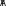
\includegraphics{week2/week2_files/figure-pdf/unnamed-chunk-2-1.pdf}

}

\end{figure}

Which would show us that \(x_1\) is associated with both \(x_2\) and
\(Y\).

Fitting a model with both \(x_1\) and \(x_2\), we would call the
prediction of \(Y\) given \(x_2\) the conditional association between
\(x_2\) conditional on (or within levels of) \(x_1\).

\begin{Shaded}
\begin{Highlighting}[]
\CommentTok{\# observe that the association flips}
\NormalTok{jtools}\SpecialCharTok{::}\FunctionTok{summ}\NormalTok{(}\FunctionTok{lm}\NormalTok{(Y }\SpecialCharTok{\textasciitilde{}}\NormalTok{ x2))}
\end{Highlighting}
\end{Shaded}

\begin{table}[!h]
\centering
\begin{tabular}{lr}
\toprule
\cellcolor{gray!6}{Observations} & \cellcolor{gray!6}{100}\\
Dependent variable & Y\\
\cellcolor{gray!6}{Type} & \cellcolor{gray!6}{OLS linear regression}\\
\bottomrule
\end{tabular}
\end{table} \begin{table}[!h]
\centering
\begin{tabular}{lr}
\toprule
\cellcolor{gray!6}{F(1,98)} & \cellcolor{gray!6}{1.30}\\
R² & 0.01\\
\cellcolor{gray!6}{Adj. R²} & \cellcolor{gray!6}{0.00}\\
\bottomrule
\end{tabular}
\end{table} \begin{table}[!h]
\centering
\begin{threeparttable}
\begin{tabular}{lrrrr}
\toprule
  & Est. & S.E. & t val. & p\\
\midrule
\cellcolor{gray!6}{(Intercept)} & \cellcolor{gray!6}{2.46} & \cellcolor{gray!6}{2.13} & \cellcolor{gray!6}{1.16} & \cellcolor{gray!6}{0.25}\\
x2 & 0.74 & 0.65 & 1.14 & 0.26\\
\bottomrule
\end{tabular}
\begin{tablenotes}
\item Standard errors: OLS
\end{tablenotes}
\end{threeparttable}
\end{table}

\begin{Shaded}
\begin{Highlighting}[]
\NormalTok{jtools}\SpecialCharTok{::}\FunctionTok{summ}\NormalTok{(}\FunctionTok{lm}\NormalTok{(Y }\SpecialCharTok{\textasciitilde{}}\NormalTok{ x1 }\SpecialCharTok{+}\NormalTok{ x2))}
\end{Highlighting}
\end{Shaded}

\begin{table}[!h]
\centering
\begin{tabular}{lr}
\toprule
\cellcolor{gray!6}{Observations} & \cellcolor{gray!6}{100}\\
Dependent variable & Y\\
\cellcolor{gray!6}{Type} & \cellcolor{gray!6}{OLS linear regression}\\
\bottomrule
\end{tabular}
\end{table} \begin{table}[!h]
\centering
\begin{tabular}{lr}
\toprule
\cellcolor{gray!6}{F(2,97)} & \cellcolor{gray!6}{89.79}\\
R² & 0.65\\
\cellcolor{gray!6}{Adj. R²} & \cellcolor{gray!6}{0.64}\\
\bottomrule
\end{tabular}
\end{table} \begin{table}[!h]
\centering
\begin{threeparttable}
\begin{tabular}{lrrrr}
\toprule
  & Est. & S.E. & t val. & p\\
\midrule
\cellcolor{gray!6}{(Intercept)} & \cellcolor{gray!6}{4.44} & \cellcolor{gray!6}{1.29} & \cellcolor{gray!6}{3.46} & \cellcolor{gray!6}{0.00}\\
x1TRUE & 1.74 & 0.13 & 13.27 & 0.00\\
\cellcolor{gray!6}{x2} & \cellcolor{gray!6}{-0.18} & \cellcolor{gray!6}{0.40} & \cellcolor{gray!6}{-0.45} & \cellcolor{gray!6}{0.66}\\
\bottomrule
\end{tabular}
\begin{tablenotes}
\item Standard errors: OLS
\end{tablenotes}
\end{threeparttable}
\end{table}

This figure shows some types of bivariate confounding:

\begin{figure}

{\centering \includegraphics{week2/images/faraway_page50.png}

}

\caption{Types of confounding from Faraway, page 50}

\end{figure}

Examples of confounding in the HERS data:

\emph{How is a woman's LDL cholesterol level associated with her body
mass index (BMI)?}

In the HERS data, women with higher BMI tend to have higher LDL levels.
However, interpreting this simple marginal association as causal might
be misleading because

\begin{itemize}
\tightlist
\item
  Older women in HERS have both lower BMI and lower LDL levels;
\item
  Ethnic background, as well as whether a woman smokes or drinks, also
  predict both higher BMI and higher LDL levels.
\end{itemize}

Thus BMI, the risk factor of interest, is associated with a number of
other factors, or potential confounders, which also predict the outcome.

\begin{Shaded}
\begin{Highlighting}[]
\FunctionTok{library}\NormalTok{(here)}
\NormalTok{hers }\OtherTok{\textless{}{-}}\NormalTok{ readr}\SpecialCharTok{::}\FunctionTok{read\_csv}\NormalTok{(}\FunctionTok{here}\NormalTok{(}\StringTok{"data/hers.csv"}\NormalTok{))}

\CommentTok{\# just visualized to see how difficult it is to observe confounding}
\NormalTok{GGally}\SpecialCharTok{::}\FunctionTok{ggpairs}\NormalTok{(hers, }\AttributeTok{columns =} \FunctionTok{c}\NormalTok{(}\StringTok{\textquotesingle{}LDL\textquotesingle{}}\NormalTok{, }\StringTok{\textquotesingle{}BMI\textquotesingle{}}\NormalTok{, }\StringTok{\textquotesingle{}age\textquotesingle{}}\NormalTok{), }\AttributeTok{alpha =}\NormalTok{ .}\DecValTok{5}\NormalTok{)}
\end{Highlighting}
\end{Shaded}

\begin{figure}[H]

{\centering \includegraphics{week2/week2_files/figure-pdf/unnamed-chunk-5-1.pdf}

}

\end{figure}

Often we will just fit separate models for each of the pairwise models:

\begin{Shaded}
\begin{Highlighting}[]
\NormalTok{simple\_summ }\OtherTok{\textless{}{-}}
  \ControlFlowTok{function}\NormalTok{(model) \{}
\NormalTok{    jtools}\SpecialCharTok{::}\FunctionTok{summ}\NormalTok{(model, }\AttributeTok{model.info =}\NormalTok{ F, }\AttributeTok{model.fit =}\NormalTok{ F)}
\NormalTok{  \}}
\FunctionTok{simple\_summ}\NormalTok{(}\FunctionTok{lm}\NormalTok{(}\AttributeTok{data =}\NormalTok{ hers, }\AttributeTok{formula =}\NormalTok{ LDL }\SpecialCharTok{\textasciitilde{}}\NormalTok{ age))}
\end{Highlighting}
\end{Shaded}

\begin{table}[!h]
\centering
\begin{threeparttable}
\begin{tabular}{lrrrr}
\toprule
  & Est. & S.E. & t val. & p\\
\midrule
\cellcolor{gray!6}{(Intercept)} & \cellcolor{gray!6}{164.83} & \cellcolor{gray!6}{7.25} & \cellcolor{gray!6}{22.73} & \cellcolor{gray!6}{0.00}\\
age & -0.30 & 0.11 & -2.74 & 0.01\\
\bottomrule
\end{tabular}
\begin{tablenotes}
\item Standard errors: OLS
\end{tablenotes}
\end{threeparttable}
\end{table}

\begin{Shaded}
\begin{Highlighting}[]
\FunctionTok{simple\_summ}\NormalTok{(}\FunctionTok{lm}\NormalTok{(}\AttributeTok{data =}\NormalTok{ hers, }\AttributeTok{formula =}\NormalTok{ LDL }\SpecialCharTok{\textasciitilde{}}\NormalTok{ BMI))}
\end{Highlighting}
\end{Shaded}

\begin{table}[!h]
\centering
\begin{threeparttable}
\begin{tabular}{lrrrr}
\toprule
  & Est. & S.E. & t val. & p\\
\midrule
\cellcolor{gray!6}{(Intercept)} & \cellcolor{gray!6}{133.19} & \cellcolor{gray!6}{3.79} & \cellcolor{gray!6}{35.11} & \cellcolor{gray!6}{0.00}\\
BMI & 0.42 & 0.13 & 3.18 & 0.00\\
\bottomrule
\end{tabular}
\begin{tablenotes}
\item Standard errors: OLS
\end{tablenotes}
\end{threeparttable}
\end{table}

\begin{Shaded}
\begin{Highlighting}[]
\FunctionTok{simple\_summ}\NormalTok{(}\FunctionTok{lm}\NormalTok{(}\AttributeTok{data =}\NormalTok{ hers, }\AttributeTok{formula =}\NormalTok{ BMI }\SpecialCharTok{\textasciitilde{}}\NormalTok{ age))}
\end{Highlighting}
\end{Shaded}

\begin{table}[!h]
\centering
\begin{threeparttable}
\begin{tabular}{lrrrr}
\toprule
  & Est. & S.E. & t val. & p\\
\midrule
\cellcolor{gray!6}{(Intercept)} & \cellcolor{gray!6}{37.40} & \cellcolor{gray!6}{1.05} & \cellcolor{gray!6}{35.78} & \cellcolor{gray!6}{0.00}\\
age & -0.13 & 0.02 & -8.48 & 0.00\\
\bottomrule
\end{tabular}
\begin{tablenotes}
\item Standard errors: OLS
\end{tablenotes}
\end{threeparttable}
\end{table}

\begin{Shaded}
\begin{Highlighting}[]
\FunctionTok{simple\_summ}\NormalTok{(}\FunctionTok{lm}\NormalTok{(}\AttributeTok{data =}\NormalTok{ hers, }\AttributeTok{formula =}\NormalTok{ LDL }\SpecialCharTok{\textasciitilde{}}\NormalTok{ BMI }\SpecialCharTok{+}\NormalTok{ age))}
\end{Highlighting}
\end{Shaded}

\begin{table}[!h]
\centering
\begin{threeparttable}
\begin{tabular}{lrrrr}
\toprule
  & Est. & S.E. & t val. & p\\
\midrule
\cellcolor{gray!6}{(Intercept)} & \cellcolor{gray!6}{151.44} & \cellcolor{gray!6}{8.77} & \cellcolor{gray!6}{17.26} & \cellcolor{gray!6}{0.00}\\
BMI & 0.37 & 0.13 & 2.78 & 0.01\\
\cellcolor{gray!6}{age} & \cellcolor{gray!6}{-0.25} & \cellcolor{gray!6}{0.11} & \cellcolor{gray!6}{-2.31} & \cellcolor{gray!6}{0.02}\\
\bottomrule
\end{tabular}
\begin{tablenotes}
\item Standard errors: OLS
\end{tablenotes}
\end{threeparttable}
\end{table}

In the marginal model \(LDL ~ BMI\), we had an effect estimate for BMI
of 0.42 vs.~0.37 in the model with both BMI and age. So we could say
there was a 12\% decrease in \(\hat \beta_{BMI}\).

A commonly used rule of thumb is that a variable is a confounder if it
changes the estimated associations of interest by \textgreater10\%.
However, this is a really arbitrary threshold, so when available
substantive knowledge should be the primary consideration for selecting
confounders a priori to any analyses. Moreover, these types of heuristic
criteria are specific to linear regression and they change for other
types of models (e.g., logistic models for binary outcomes).

We could condition on a few more variables that we might suspect are
possible confounders:

\begin{Shaded}
\begin{Highlighting}[]
\FunctionTok{simple\_summ}\NormalTok{(}\FunctionTok{lm}\NormalTok{(LDL }\SpecialCharTok{\textasciitilde{}}\NormalTok{ BMI }\SpecialCharTok{+}\NormalTok{ age }\SpecialCharTok{+}\NormalTok{ nonwhite }\SpecialCharTok{+}\NormalTok{ drinkany }\SpecialCharTok{+}\NormalTok{ smoking, }\AttributeTok{data =}\NormalTok{ hers))}
\end{Highlighting}
\end{Shaded}

\begin{table}[!h]
\centering
\begin{threeparttable}
\begin{tabular}{lrrrr}
\toprule
  & Est. & S.E. & t val. & p\\
\midrule
\cellcolor{gray!6}{(Intercept)} & \cellcolor{gray!6}{147.32} & \cellcolor{gray!6}{9.26} & \cellcolor{gray!6}{15.91} & \cellcolor{gray!6}{0.00}\\
BMI & 0.36 & 0.13 & 2.68 & 0.01\\
\cellcolor{gray!6}{age} & \cellcolor{gray!6}{-0.19} & \cellcolor{gray!6}{0.11} & \cellcolor{gray!6}{-1.68} & \cellcolor{gray!6}{0.09}\\
nonwhiteyes & 5.22 & 2.32 & 2.25 & 0.02\\
\cellcolor{gray!6}{drinkanyyes} & \cellcolor{gray!6}{-2.72} & \cellcolor{gray!6}{1.50} & \cellcolor{gray!6}{-1.82} & \cellcolor{gray!6}{0.07}\\
\addlinespace
smokingyes & 4.75 & 2.21 & 2.15 & 0.03\\
\bottomrule
\end{tabular}
\begin{tablenotes}
\item Standard errors: OLS
\end{tablenotes}
\end{threeparttable}
\end{table}

The effect for \(\hat \beta_{BMI}\) didn't change very much, so we can
presume that these additional variables are not meaningful confounders
of the \(LDL ~ BMI\) relationship.

\hypertarget{interaction}{%
\section{Interaction}\label{interaction}}

We may be interested in a model with \emph{interaction effects}:

\[ \mathbb E(Y_i) = \beta_0 + \beta_1 x_{i1} + \beta_3 x_{i1} x_{i2}\]

We can alternatively view this model as

\[ \mathbb E(Y_i) = (\beta_0 + \beta_2 x_{i2}) + (\beta_1 + \beta_3 x_{i2})x_{i1} + \epsilon_i.\]

(or switch the roles of \(x_{i1}\) and \(x_{i2}\). Interactions are also
sometimes referred to as \emph{effect-modification}.

Generally it's considered best practice whenever including interaction
terms to include the main-effects for any interacted variables as well.
Sometimes in economics literature, main effects may be referred to as
``constitutive effects''.

\hypertarget{statin-use-example}{%
\subsection{Statin-Use Example}\label{statin-use-example}}

For example, we might ask if the association between LDL and BMI differ
between those who take statins (cholesterol lowering medications)
vs.~those who do not?

We center BMI so that the Statin coefficient is meaningful.

\begin{Shaded}
\begin{Highlighting}[]
\NormalTok{hers}\SpecialCharTok{$}\NormalTok{BMI\_centered }\OtherTok{\textless{}{-}}\NormalTok{ hers}\SpecialCharTok{$}\NormalTok{BMI }\SpecialCharTok{{-}} \FunctionTok{mean}\NormalTok{(hers}\SpecialCharTok{$}\NormalTok{BMI, }\AttributeTok{na.rm=}\ConstantTok{TRUE}\NormalTok{)}
\FunctionTok{simple\_summ}\NormalTok{(}\FunctionTok{lm}\NormalTok{(}
\NormalTok{  LDL }\SpecialCharTok{\textasciitilde{}}\NormalTok{ BMI\_centered }\SpecialCharTok{*}\NormalTok{ statins }\SpecialCharTok{+} 
\NormalTok{    age }\SpecialCharTok{+}\NormalTok{ smoking }\SpecialCharTok{+}\NormalTok{ drinkany }\SpecialCharTok{+}\NormalTok{ nonwhite,}
  \AttributeTok{data =}\NormalTok{ hers}
\NormalTok{))}
\end{Highlighting}
\end{Shaded}

\begin{table}[!h]
\centering
\begin{threeparttable}
\begin{tabular}{lrrrr}
\toprule
  & Est. & S.E. & t val. & p\\
\midrule
\cellcolor{gray!6}{(Intercept)} & \cellcolor{gray!6}{162.41} & \cellcolor{gray!6}{7.58} & \cellcolor{gray!6}{21.42} & \cellcolor{gray!6}{0.00}\\
BMI\_centered & 0.58 & 0.16 & 3.64 & 0.00\\
\cellcolor{gray!6}{statinsyes} & \cellcolor{gray!6}{-16.25} & \cellcolor{gray!6}{1.47} & \cellcolor{gray!6}{-11.07} & \cellcolor{gray!6}{0.00}\\
age & -0.17 & 0.11 & -1.56 & 0.12\\
\cellcolor{gray!6}{smokingyes} & \cellcolor{gray!6}{3.11} & \cellcolor{gray!6}{2.17} & \cellcolor{gray!6}{1.44} & \cellcolor{gray!6}{0.15}\\
\addlinespace
drinkanyyes & -2.08 & 1.47 & -1.42 & 0.16\\
\cellcolor{gray!6}{nonwhiteyes} & \cellcolor{gray!6}{4.07} & \cellcolor{gray!6}{2.28} & \cellcolor{gray!6}{1.79} & \cellcolor{gray!6}{0.07}\\
BMI\_centered:statinsyes & -0.70 & 0.27 & -2.61 & 0.01\\
\bottomrule
\end{tabular}
\begin{tablenotes}
\item Standard errors: OLS
\end{tablenotes}
\end{threeparttable}
\end{table}

Another option not-covered in class is to use the \texttt{/} operator to
create a BMI effect within the yes/no levels of statins:

check \texttt{?formula.terms} for an explanation of the \texttt{/}
operator:

``The \texttt{/} operator provides a shorthand, so that \texttt{a\ /\ b}
is equivalent to \texttt{a\ +\ b\ \%in\%\ a}.''

\begin{Shaded}
\begin{Highlighting}[]
\NormalTok{lm.ldl.interact }\OtherTok{\textless{}{-}} \FunctionTok{lm}\NormalTok{(}
\NormalTok{  LDL }\SpecialCharTok{\textasciitilde{}}\NormalTok{ statins }\SpecialCharTok{/}\NormalTok{ BMI\_centered }\SpecialCharTok{+} 
\NormalTok{    age }\SpecialCharTok{+}\NormalTok{ smoking }\SpecialCharTok{+}\NormalTok{ drinkany }\SpecialCharTok{+}\NormalTok{ nonwhite,}
  \AttributeTok{data =}\NormalTok{ hers}
\NormalTok{)}
\FunctionTok{simple\_summ}\NormalTok{(lm.ldl.interact)}
\end{Highlighting}
\end{Shaded}

\begin{table}[!h]
\centering
\begin{threeparttable}
\begin{tabular}{lrrrr}
\toprule
  & Est. & S.E. & t val. & p\\
\midrule
\cellcolor{gray!6}{(Intercept)} & \cellcolor{gray!6}{162.41} & \cellcolor{gray!6}{7.58} & \cellcolor{gray!6}{21.42} & \cellcolor{gray!6}{0.00}\\
statinsyes & -16.25 & 1.47 & -11.07 & 0.00\\
\cellcolor{gray!6}{age} & \cellcolor{gray!6}{-0.17} & \cellcolor{gray!6}{0.11} & \cellcolor{gray!6}{-1.56} & \cellcolor{gray!6}{0.12}\\
smokingyes & 3.11 & 2.17 & 1.44 & 0.15\\
\cellcolor{gray!6}{drinkanyyes} & \cellcolor{gray!6}{-2.08} & \cellcolor{gray!6}{1.47} & \cellcolor{gray!6}{-1.42} & \cellcolor{gray!6}{0.16}\\
\addlinespace
nonwhiteyes & 4.07 & 2.28 & 1.79 & 0.07\\
\cellcolor{gray!6}{statinsno:BMI\_centered} & \cellcolor{gray!6}{0.58} & \cellcolor{gray!6}{0.16} & \cellcolor{gray!6}{3.64} & \cellcolor{gray!6}{0.00}\\
statinsyes:BMI\_centered & -0.12 & 0.22 & -0.54 & 0.59\\
\bottomrule
\end{tabular}
\begin{tablenotes}
\item Standard errors: OLS
\end{tablenotes}
\end{threeparttable}
\end{table}

How do we interpret them? Often the simplest way is to just visualize
them.

\begin{Shaded}
\begin{Highlighting}[]
\CommentTok{\# install.packages("interactions")}
\NormalTok{interactions}\SpecialCharTok{::}\FunctionTok{interact\_plot}\NormalTok{(lm.ldl.interact,}
                            \AttributeTok{pred =}\NormalTok{ BMI\_centered, }\AttributeTok{modx =}\NormalTok{ statins,}
                            \AttributeTok{interval =} \ConstantTok{TRUE}\NormalTok{)}
\end{Highlighting}
\end{Shaded}

\begin{figure}[H]

{\centering \includegraphics{week2/week2_files/figure-pdf/unnamed-chunk-10-1.pdf}

}

\end{figure}

\emph{Question:} How would we interpret the magnitude of an interaction
between 2 continuous variables?

The coefficient estimate for an interaction with two continuous effects
is the change in the \(x_1 \sim Y\) slope corresponding to a 1-unit
change in \(x_2\).

\bookmarksetup{startatroot}

\hypertarget{estimation}{%
\chapter{Estimation}\label{estimation}}

\hypertarget{matrix-representation-of-multiple-linear-regression}{%
\section{Matrix Representation of Multiple Linear
Regression}\label{matrix-representation-of-multiple-linear-regression}}

I will use math bolding \emph{once} and then give up on it. Do not
expect more from me. It is too much of a pain to write in every line.

\[ \pmb Y = \pmb X \pmb \beta + \pmb \epsilon \]

\[ \pmb Y = \left[ \begin{array}{c} Y_1 \\ Y_2 \\ \vdots \\ Y_n \end{array}  \right],
\quad \pmb X = \left[ \begin{array}{ccccc} 1 & x_{11} & x_{12} & \cdots & x_{1p} \\
1 & x_{21} & x_{22} & \cdots & x_{2p} \\
\vdots & \vdots & \vdots & \ddots & \vdots \\
1 & x_{n1} & x_{n2} & \cdots & x_{np} \\
\end{array} \right], \]

\[ \pmb \beta = \left[ \begin{array}{c} \beta_1 \\ \beta_2 \\ \vdots \\ \beta_n \end{array}  \right],
\quad \pmb \epsilon = \left[ \begin{array}{c} \epsilon_1 \\ \epsilon_2 \\ \vdots \\ \epsilon_n \end{array}  \right].\]

Now we can write (under the usual assumptions on \(\epsilon_i\)), we can
alternatively write \(\mathbb E(\pmb Y) = \pmb X \pmb \beta\).

This marks the spot when I shall give up on bolding vectors and
matrices.

\hypertarget{how-should-we-estimate-hat-beta}{%
\section{\texorpdfstring{How should we estimate
\(\hat \beta\)?}{How should we estimate \textbackslash hat \textbackslash beta?}}\label{how-should-we-estimate-hat-beta}}

Thus far we haven't made any distributional assumptions.

Without distributional assumptions, one way forward is to simply find
the estimate \(\hat \beta\) that results in \(X \hat \beta\) as close as
possible to the observed \(y\). (Note teh change to a lowercase \(y\)
when referring to observed values in the sample rather than a random
variable).

Using Euclidean distance, the distance between the vectors \(y\) and
\(X \beta\) is

\[ d(y, X\beta) = \sqrt{(y-X\beta)'(y-X\beta)}.\]

We generally prefer not to work with square roots and since squaring is
a momotone transformation for values on \(\mathbb R^+\), the value that
minimizes \(d(y, X\beta)\) will also minimize \(d(y,X\beta)^2\).

\[S(\beta) = SSE = d(y,X\beta)^2 = (y-X\beta)'(y-X\beta)\]
\[ = y'y - 2y'X\beta + \beta' X' X \beta\]

The values of \(\beta\) that minimize \(S(\beta)\) are called least
squares estimates or ordinatry least squares (OLS) estimates.

OLS has been around since at least the early 1800s and variously
attributed to Gauss, Laplace, Legendre, etc.. A lot of the properties of
estimators obtained in this way were proven by Gauss.

See Stephen Stigler's \emph{Gauss and the Invention of Least Squares}
\url{https://www.jstor.org/stable/2240811}.

To find OLS estimates, we (1) compute the gradient of \(S(\beta)\), (2)
set the equation to zero, and (3) solve for \(\beta\).

\[ \frac{\partial S(\beta)}{\partial \beta } = -2X'y + 2X'X\beta \stackrel{set}{=} 0\]
\[ = -2X'(y-X\beta) = 0\]

This gives us the least squares normal equations:

\[ X'X \hat \beta = X' y\]

Normal equations have a relationship to geometry that ``we'' won't
expand on further. Except I will! See
\url{https://stats.stackexchange.com/a/305748/174809}

\begin{figure}

{\centering \includegraphics[width=5in,height=\textheight]{week2/standalone_figures/normal_equation_projection/normal_equation_projection.svg}

}

\end{figure}

Multiply each side by \((X'X)^{-1}\) to obtain:
\[\hat \beta = (X'X)^{-1}X'y\] provided \((X'X)^{-1}\) exists (it will
if predictors are linearly independent.

This is a good equation to commit to memory.

(About now is a good time to note that \(X\) is capitalized because it's
a matrix, not because it's a random variable).

\hypertarget{simple-linear-regression-setting}{%
\section{Simple Linear Regression
Setting}\label{simple-linear-regression-setting}}

\[\hat \beta_1 = 
\frac{\sum_{i=1}^n (x_i - \bar x)(y_i - \bar y}{\sum_{i=1}^n (x_i - \bar x)^2} = \frac{\widehat{\text{Cov}} (x,y)}{\left(\widehat{\text{sd}}(x)\right)^2} = 
\hat \rho_{xy} \left( \frac{\widehat{\text{sd}}(y)}{\widehat{\text{sd}}(x)} \right)\]

\[\hat{\beta_0} = \bar y - \hat \beta_1 \bar x.\]

Using these estimates, we get a {fitted value} for the \(i\)th
observation and a residual for it.

\hypertarget{properties-of-least-squares-estimates}{%
\section{Properties of Least Squares
Estimates}\label{properties-of-least-squares-estimates}}

\(\hat \beta\) is an unbiased estimator of \(\beta\).

\[\mathbb E(\hat \beta) = \mathbb E[\underbrace{(X'X)^{-1} X'}_{A} y] = (X'X)^{-1} X'X \beta = \beta\]

The variance of \(\hat \beta\) is expressed by the
\textbf{variance-covariance matrix}.

\[\text{Var}(\hat \beta) = (X'X)^{-1} X' \text{Var}(Y) X (X'X)^{-1}\]
\[ = \sigma^2 (X'X)^{-1}\]

If we let \(D = (X'X)^{-1}\), the variance of
\(\hat \beta_j = \sigma D_{jj}\) and the covariance between
\(\hat \beta_i\) and \(\hat \beta_j\) is \(\sigma^2 D_{ij}\).

\bookmarksetup{startatroot}

\hypertarget{lab}{%
\chapter{Lab}\label{lab}}

Properties of estimators that we want:

\begin{itemize}
\tightlist
\item
  Consistency \(\hat \beta \stackrel{p}{\to} \beta\)
\item
  Minimal bias \(\hat \beta - \beta\)
\item
  Computability
\item
  Minimal \(\text{Var}(\hat \beta)\)
\end{itemize}

Recommended reading: the Matrix Cookbook

\hypertarget{basic-matrix-rules}{%
\subsection{Basic Matrix Rules}\label{basic-matrix-rules}}

\begin{itemize}
\tightlist
\item
  \((AB)^T = B^TA^T\)
\item
  If \(C\) and \(D\) are invertible, \((CD)^{-1} = D^{-1}C^{-1}\)
\item
  \((C^{-1})^T = (C^T)^{-1}\)
\end{itemize}

Note that we can do matrix calculus too

Let \(z\) be a vector.

\[ \frac{\partial Az}{\partial z} = A\]

\[ \frac{\partial}{\partial z} \left[ \begin{array}{cc} a_1 & a_2 \\ a_3 & a_4 \end{array} \right] \left[ \begin{array}{l} z_1 \\ z_2 \end{array} \right] = 
\left[ \begin{array}{cc} \frac{\partial}{\partial z_1} z_1 + a_1 + z_2 + a_2 & \frac{\partial}{\partial z_2} z_1 a_1 + z_2 a_2 \\ 
\frac{\partial}{\partial z_1} z_1 + a_3 + z_2 + a_4 & 
\frac{\partial}{\partial z_2} z_1 + a_3 + z_2 + a_4 \end{array}
\right] = 
\left[ \begin{array}{cc} a_1 & a_2 \\ a_3 & a_4 \end{array} \right]\]

\[ \frac{\partial z^T B}{\partial z} = B^T\]

If \(C\) is symmetric,

\[\frac{\partial z^T C z}{\partial z} = 2z^T C \]

Probability results:

\[\mathbb E(AZ) = A \mathbb E(Z)\]
\[\text{Var}(AZ) = A \text{Var}(Z) A^T\]

\textbf{Derive the least squares estimate for \(\beta\).}

We want to minimize \(Y - X\beta\), and hence we want to set
\[\frac{\partial}{\partial \beta} (Y - X\beta)^T(Y - X\beta) = 0\]

\[ = \frac{\partial}{\partial \beta} (Y^T - X\beta^T)(Y - X\beta)\]

\[ = \frac{\partial}{\partial \beta} Y^T Y - Y^T X \beta - (X\beta)^TY + (X\beta)^T(X\beta)\]

\[ = -Y^TX - Y^TX  + 2\beta^TX^TX = 0\]

\[ \hat \beta = (X^TX)^{-1}X^TY\]

\hypertarget{how-do-we-write-the-hat-y-and-estimated-residuals}{%
\subsection{\texorpdfstring{How do we write the \(\hat Y\) and estimated
residuals?}{How do we write the \textbackslash hat Y and estimated residuals?}}\label{how-do-we-write-the-hat-y-and-estimated-residuals}}

\[\hat Y = X \hat \beta = \underbrace{X(X^TX)^{-1}X^T}_{\text{called the hat matrix}}Y = HY\]

\[\hat \epsilon = Y - \hat Y = (I_n - H)Y\]

\hypertarget{find-the-expectation-and-variance-covariance-matrix-of-hat-beta}{%
\subsection{\texorpdfstring{Find the expectation and variance-covariance
matrix of
\(\hat \beta\)}{Find the expectation and variance-covariance matrix of \textbackslash hat \textbackslash beta}}\label{find-the-expectation-and-variance-covariance-matrix-of-hat-beta}}

\[\mathbb E(\hat \beta) = \mathbb E((X^TX)^{-1}X^TY) = (X^TX)^{-1}X^T \mathbb E(Y)\]
\[ = \cancel{(X^TX)^{-1}X^TX} \beta = \beta\]

\[\text{Var}(\hat \beta) = (X^TX)^{-1}X^T \sigma^2 I_n X(X^TX)^{-1} \sigma^2 (X^TX)^{-1}\]

\hypertarget{how-do-estimates-from-the-two-methods-differ}{%
\subsection{How do estimates from the two methods
differ?}\label{how-do-estimates-from-the-two-methods-differ}}

We get the same \(\hat \beta\) estimates.

We get something that's proportional to
\(\exp{-\frac{1}{2}(Y-X\beta)^T(Y-X\beta)}\).

These are basically the same.

\hypertarget{simulation-code-for-a-confounder}{%
\subsection{Simulation Code for a
Confounder}\label{simulation-code-for-a-confounder}}

Suppose we have a scenario where

\begin{itemize}
\tightlist
\item
  \(X_1 \sim \text{Uniform}(0,5)\)
\item
  \(X_2|X_1 \sim \text{Normal}(x_1, 1)\)
\item
  \(Y|X_1, X_2 \sim \text{Normal}(2x_1 + 0.01x_2 + 2, 1)\)
\end{itemize}

Now consider two regression models:

\begin{enumerate}
\def\labelenumi{\arabic{enumi}.}
\tightlist
\item
  \(Y_i = \beta_0 + \beta_2 X_{i2} + \varepsilon_i\)
\item
  \(Y_i = \beta_0 + \beta_1 X_{i1} + \beta_2X_{i2} + \varepsilon_i\)
\end{enumerate}

Compare what happens to the \(\beta\) estimates from both regressions.

\begin{Shaded}
\begin{Highlighting}[]
\NormalTok{simulate }\OtherTok{\textless{}{-}} \ControlFlowTok{function}\NormalTok{(n) \{}
\NormalTok{  X1 }\OtherTok{\textless{}{-}} \FunctionTok{runif}\NormalTok{(n, }\DecValTok{0}\NormalTok{, }\DecValTok{5}\NormalTok{)}
\NormalTok{  X2 }\OtherTok{\textless{}{-}} \FunctionTok{rnorm}\NormalTok{(n, X1)}
\NormalTok{  Y }\OtherTok{\textless{}{-}} \FunctionTok{rnorm}\NormalTok{(n, }\DecValTok{2}\SpecialCharTok{*}\NormalTok{X1 }\SpecialCharTok{+}\NormalTok{ .}\DecValTok{01}\SpecialCharTok{*}\NormalTok{X2 }\SpecialCharTok{+} \DecValTok{2}\NormalTok{)}
  
\NormalTok{  model1 }\OtherTok{\textless{}{-}} \FunctionTok{lm}\NormalTok{(Y }\SpecialCharTok{\textasciitilde{}}\NormalTok{ X2)}
\NormalTok{  model2 }\OtherTok{\textless{}{-}} \FunctionTok{lm}\NormalTok{(Y }\SpecialCharTok{\textasciitilde{}}\NormalTok{ X1 }\SpecialCharTok{+}\NormalTok{ X2)}
  
  \FunctionTok{return}\NormalTok{(}\FunctionTok{c}\NormalTok{(}\AttributeTok{omit =}\NormalTok{ model1}\SpecialCharTok{$}\NormalTok{coefficients[[}\StringTok{\textquotesingle{}X2\textquotesingle{}}\NormalTok{]], }
           \AttributeTok{full =}\NormalTok{ model2}\SpecialCharTok{$}\NormalTok{coefficients[[}\StringTok{\textquotesingle{}X2\textquotesingle{}}\NormalTok{]]))}
\NormalTok{\}}

\NormalTok{output }\OtherTok{\textless{}{-}} \FunctionTok{replicate}\NormalTok{(}\DecValTok{1000}\NormalTok{, }\FunctionTok{simulate}\NormalTok{(}\DecValTok{100}\NormalTok{))}
\FunctionTok{hist}\NormalTok{(output[}\StringTok{\textquotesingle{}omit\textquotesingle{}}\NormalTok{,])}
\end{Highlighting}
\end{Shaded}

\begin{figure}[H]

{\centering \includegraphics{week2/week2_files/figure-pdf/unnamed-chunk-12-1.pdf}

}

\end{figure}

\begin{Shaded}
\begin{Highlighting}[]
\FunctionTok{hist}\NormalTok{(output[}\StringTok{\textquotesingle{}full\textquotesingle{}}\NormalTok{,])}
\end{Highlighting}
\end{Shaded}

\begin{figure}[H]

{\centering \includegraphics{week2/week2_files/figure-pdf/unnamed-chunk-12-2.pdf}

}

\end{figure}

\begin{Shaded}
\begin{Highlighting}[]
\FunctionTok{hist}\NormalTok{(output, }\AttributeTok{breaks =} \DecValTok{50}\NormalTok{)}
\end{Highlighting}
\end{Shaded}

\begin{figure}[H]

{\centering \includegraphics{week2/week2_files/figure-pdf/unnamed-chunk-12-3.pdf}

}

\end{figure}

\hypertarget{comparing-ols-vs.-mle-estimates}{%
\subsection{Comparing OLS vs.~MLE
estimates}\label{comparing-ols-vs.-mle-estimates}}

We want to know why this estimator derived from the maximum likelihood
estimation approach in which we try to maximize the multivariate normal
distriution

\[{\displaystyle (2\pi )^{-k/2}\det({\boldsymbol {\Sigma }})^{-1/2}\,\exp \left(-{\frac {1}{2}}(\mathbf {x} -{\boldsymbol {\mu }})^{\mathsf {T}}{\boldsymbol {\Sigma }}^{-1}(\mathbf {x} -{\boldsymbol {\mu }})\right)}\]

is the same as the OLS estimator?

Basically these elements are just constant, and the effect of the
exponential function isn't important (see next line).

\[{\cancel{\displaystyle (2\pi )^{-k/2}}\cancel{\det({\boldsymbol {\Sigma }})^{-1/2}}\,\cancel{\exp} \left(\cancel{-{\frac {1}{2}}}(\mathbf {x} -{\boldsymbol {\mu }})^{\mathsf {T}}{\boldsymbol {\Sigma }}^{-1}(\mathbf {x} -{\boldsymbol {\mu }})\right),}\]

We're trying to maximize the likelihood,

\(\ell (\mu|x)= \log (\exp \left(-{\frac {1}{2}}(\mathbf {x} -{\boldsymbol {\mu }})^{\mathsf {T}}{\boldsymbol {\sigma^2 I_n }}^{-1}(\mathbf {x} -{\boldsymbol {\mu }})\right),\)

which shows why we can cancel away the \(\log \exp\).

\bookmarksetup{startatroot}

\hypertarget{week-3}{%
\chapter{Week 3}\label{week-3}}

Recap:

Recall that we can write in matrix notation:

\[Y = X\beta + \epsilon\]

\[\mathbb E(Y) = X\beta\]

Assuming that \(E(\epsilon) = 0\) and
\(\text{Var}(\epsilon) = \sigma^2I\).

Remember how we derived the formula for \(\hat \beta_{OLS}\)? We set
\(\frac{\partial}{\partial \beta} SSE(\beta) \stackrel{set}{=} 0\)?

Calculating that out, we find that
\[ \frac{\partial}{\partial \beta} SSE(\beta) = -2X'y + 2X'X\beta, \]
\[ \Longrightarrow X'X \hat \beta = X' y\]
\[ \Longrightarrow \hat \beta_{OLS} = (X'X)^{-1}X'y\]

For standard linear regression (SLR), OLS slope estimates are a scaled
correlation coefficient.

Recall that the vector of random values is a variance-covariance matrix.

Last time we showed that \(\hat \beta\) is an unbiased estimator for
\(\beta\) when we saw that

\[\mathbb E(\hat \beta) = \mathbb E[\underbrace{(X'X)^{-1} X'}_{A} y] = (X'X)^{-1} X'X \beta = \beta\]

The variance of \(\hat \beta\) is expressed as the variance-covariance
matrix

\[\text{Var}(\hat \beta) = (X'X)^{-1} X' \text{Var}(Y) X (X'X)^{-1}\]
\[ = \sigma^2 (X'X)^{-1}\]

If we let \(D = (X'X)^{-1}\), the variance of
\(\hat \beta_j = \sigma D_{jj}\) and the covariance between
\(\hat \beta_i\) and \(\hat \beta_j\) is \(\sigma^2 D_{ij}\).

How would we get to this result?

We are using a shorthand where we denote \((X'X)^TX' = A\), and now
we're just looking at the \(\text{Var}(AY)\). When we are working with
the matrix-variance formula, we can rewrite
\(\text{Var}(AY) = A\text{Var}(Y)A'\).

Plugging in the formula for \(A\), we get to the above.

Remember we said that \(\text{Var}(\epsilon) = \sigma^2\) and
\(Y = X\beta + \epsilon\) where the only randomness comes from
\(\epsilon\). In other words

\[\text{Var}(\hat \beta) = (X'X)^{-1} X' \text{Var}(Y) X (X'X)^{-1}\]
\[ = (X'X)^{-1} X' \text{Var}(X\beta + \epsilon) X (X'X)^{-1}\]
\[ = (X'X)^{-1} X' \text{Var}(\epsilon) X (X'X)^{-1}\]
\[ = (X'X)^{-1} X' \sigma^2 I X (X'X)^{-1}\]
\[ = \sigma^2 (X'X)^{-1} X' I X (X'X)^{-1}\]
\[ = \sigma^2 \cancel{(X'X)^{-1} X' X }\underbrace{(X'X)^{-1}}_{\stackrel{set}{=}D}.\]

\hypertarget{gauss-markov-theorem}{%
\subsection{Gauss-Markov Theorem}\label{gauss-markov-theorem}}

Under the standard linear assumptions, \(\hat \beta_{OLS}\) is the best
linear unbiased estimator (BLUE) for \(\beta\).

Linear unbiased estimator: \(\hat \beta_{OLS}\) is a linear combination
of the observed \(y\) values (given that \(\hat \beta = (X'X)^{-1}X'y\)
is a matrix of constants times a vector \(y\)) and is an unbiased
estimator.

It's ``best'' in the sense that it is the lowest variance (most
precise).

So the Gauss Markov Theorem tells us that among all linear, unbiased
estimators of \(\beta\), \(\hat \beta_{OLS}\) has the lowest variance.

\hypertarget{simple-linear-regression-as-a-special-case}{%
\subsection{Simple Linear Regression as a Special
Case}\label{simple-linear-regression-as-a-special-case}}

The least squares estimators \(\hat \beta_0\) and \(\hat \beta_1\) can
be expressed as

\[\hat \beta_0 = \sum_{i=1}^n l_i y_i, \quad \hat \beta_1 = \sum_{i=1}^n k_i y_i,\]

where
\(l_i = \frac{1}{n} - \frac{\bar x(x_i - \bar x)}{\sum_{i=1}^n (x_i - \hat x)^2},\)
and \(k_i = \frac{(x_i - \bar x)}{\sum_{i=1}^n (x_i - \bar x)^2}\).

\hypertarget{variance-of-ls-estimators}{%
\subsubsection{Variance of LS
Estimators}\label{variance-of-ls-estimators}}

\[\text{Var}(\hat \beta_0) = \sigma \left\{ \frac{1}{n} + \frac{\bar x^2}{\sum_{i=1}^n (x_i-\bar x)^2}\right\},\]
\[\text{Var}(\hat \beta_1) = \sigma \left\{\frac{1}{\sum_{i=1}^n (x_i-\bar x)^2}\right\},\]
\[\text{Cov}(\hat \beta_0, \hat \beta_1) = \sigma \left\{ - \frac{\bar x}{\sum_{i=1}^n (x_i-\bar x)^2}\right\}.\]

The variance-covariance matrix is

\[\text{Var}(\hat \beta) = \sigma(X'X)^{-1} = \left[ \begin{array}{cc} \text{Var}(\hat \beta_0) & \text{Cov}(\hat \beta_0, \hat \beta_1) \\ \text{Cov}(\hat \beta_0, \hat \beta_1) & \text{Var}(\hat \beta_1) \end{array} \right].\]

\hypertarget{estimation-of-sigma2}{%
\subsubsection{\texorpdfstring{Estimation of
\(\sigma^2\)}{Estimation of \textbackslash sigma\^{}2}}\label{estimation-of-sigma2}}

In order to estimate \(\text{Var}(\hat \beta)\), we need an estimator of
\(\sigma^2\):

We base this on the sum of squared errors (SSE):

\[SSE = (y - X\hat\beta)'(y-X\hat \beta)\]
\[ = \sum_{i=1}^n(y_i-x'_i\hat\beta)^2\]
\[ = \sum_{i=1}^n (\hat \epsilon_i)^2\]

\[\hat \sigma^2 = MSE = \frac{SSE}{n - p - 1}.\]

This estimator \(\hat \sigma^2\) is an unbiased estimator.

The \(n-p-1\) in the denominator is because we estimate \(p+1\)
parameters and we divide by the degrees of freedom, which is
\(n - \text{\# things we had to estimate}\). The Kutner book has a more
rigorous presentation of why this is the right amount to divide by.

\hypertarget{normality-assumption}{%
\subsection{Normality assumption}\label{normality-assumption}}

If we are willing to make the stronger assumption that
\(\epsilon_i \stackrel{iid}{\sim} \mathcal N(0, \sigma^2)\), then we can
perform inference on \(\beta\).

First note that
\(\epsilon_i \stackrel{iid}{\sim} \mathcal N(0, \sigma^2) \Longrightarrow Y_i \stackrel{ind}{\sim} \mathcal N(x_i'\beta, \sigma^2)\),
such that

\[f_Y(y_i|\beta, \sigma^2) = \frac{1}{\sqrt{2\pi\sigma^2}} \exp\left[ -\frac{1}{2\sigma^2} (y_i - x_i'\beta)^2\right]\]

Notice that the \(Y_i\) values are independent but not identically
distributed.

Before we were just assuming that the \(\epsilon\) values were
uncorrelated, which in the special case of the normal distribution
implies independence, but this isn't necessarily so for other
distributions.

We can then use maximum likelihood techniques to obtain
\[\hat \beta_{MLE} \sim MVN_{p+1} \left[ \beta, \sigma^2 (X'X)^{-1} \right].\]

\hypertarget{joint-density}{%
\subsection{Joint Density}\label{joint-density}}

Recap of maximum likelihood estimation.

In general, suppose we have data \(Y_1, ..., Y_n\), which are
independent random variables with \(Y_i\) having probability density
function \[f_Y(y_i|\theta)\] where \(\theta\) is a vector of unknown
parameters.

Then the joint density function of all the \(y_i\) given \(\theta\) is
the product of the individual densities

\[f(y_1, ..., y_n|\theta) = \prod_{i=1}^n f_Y(y_i|\theta).\]

\hypertarget{likelihood-functions}{%
\subsubsection{Likelihood Functions}\label{likelihood-functions}}

The {likelihood function} of \(\theta\) given the data has the same form
as the joint pdf:

\[\mathcal L(\theta|y_1,...,y_n) = f(y_1, ..., y_n|\theta) = \prod_{i=1}^n f_Y(y_i|\theta).\]

Of course this looks exactly the same as the joint density of the
\(Y_i\) values, but instead this is a function of \(\theta\) instead of
a function of the \(y_i\) values.

Once you take a random sample of size \(n\), the \(y_i\) values are
known, and the likelihood is considered as a function of unknown
parameter \(\theta\).

The likelihood function should still integrate to 1.

The {MLE} of \(\theta\) is the value \(\hat \theta\) that maximizes the
likelihood

\[\mathcal L(\theta | y_1, ..., y_n)\]

as a function of \(\theta\).

The value \(\hat \theta\) that maximizes \(\mathcal L(\theta)\) also
maximizes

\[\ell(\theta | y_1, ..., y_n) = \log \mathcal L(\theta | y_1, ..., y_n).\]

\hypertarget{solving-for-mle}{%
\subsubsection{Solving for MLE}\label{solving-for-mle}}

\[ \frac{\partial \ell}{\partial \theta} \stackrel{set}{=} 0,\]

and technically we're going to need to check that this is a maximum as
opposed to a minimum, and we'll do so by checking that

\[\left[ \frac{\partial^2 \ell}{\partial \theta^2} \right]_{\theta = \hat \theta} < 0.\]

If we were in a matrix setting instead of a vector setting, we'd need to
check that the matrix is negative definite for a maximum, or positive
definite for a minimum.

The negative of the second derivative,

\[\frac{-\partial^2 \ell(\theta | y_1, ..., y_n)}{\partial \theta^2},\]

is called the {information}.

\hypertarget{returning-to-mle-for-regression}{%
\subsubsection{Returning to MLE for
Regression}\label{returning-to-mle-for-regression}}

Thus in the linear regression setting if we assume
\(\epsilon_i \stackrel{iid}{\sim} \mathcal N(0, \sigma^2),\) then
\(Y_i \stackrel{ind}{\sim} \mathcal N(x'_i\beta, \sigma^2)\) and
\[f_Y(y_i|\beta, \sigma^2) = \frac{1}{\sqrt{2\pi\sigma^2}} \exp \left[ -\frac{1}{2\sigma^2} (y_i - x_i'\beta)^2\right]\]

\[\mathcal L(\beta, \sigma^2 | y_1, ..., y_n) = \prod_{i=1}^n f_Y(y_i|\beta, \sigma^2),\]

and

\[\mathcal L(\beta, \sigma^2|y_1, ..., y_n) = \left( \frac{1}{\sqrt{2\pi\sigma^2}}\right)^n
\exp \left[ - \frac{1}{2\sigma^2} \sum_{i=1}^n (y_i - x_i'\beta)^2 \right]\]
\[= \left( \frac{1}{\sqrt{2\pi\sigma^2}}\right)^n
\exp \left[ - \frac{1}{2\sigma^2} (y - X\beta)'(y-X\beta) \right].\]

Turning to the log-likelihood function:

\[\ell(\beta, \sigma^2 | y_1, ..., y_n) \propto \cancel{-n/2\log(\sigma^2)} \underbrace{- \frac{1}{2\sigma^2} (y-X\beta)'(y-X\beta)}_{= \frac{-1}{2\sigma^2} S(\beta)}.\]

The values that maximize this log-likelihood with respect to \(\beta\),
call them \(\hat \beta_{MLE}\) are the same as those that minimize
\(S(\hat \beta)\), i.e.,

\[\hat \beta_{MLE} = (X'X)^{-1}X'y\]

and it's straightforward to show that

\[\hat \beta_{MLE} \sim MVN_{p+1}\left[ \beta, \sigma^2(X'X)^{-1} \right].\]

\hypertarget{sigma2_mle}{%
\subsubsection{\texorpdfstring{\(\sigma^2_{MLE}\)}{\textbackslash sigma\^{}2\_\{MLE\}}}\label{sigma2_mle}}

While the estimates for \(\hat \beta\) are the same for OLS vs.~MLE, we
have that
\[\hat \sigma^2_{MLE} = \frac{1}{n}(y-X\hat\beta)'(y-X\hat\beta) = \frac{(n-p-1)}{n}MSE\]

So of note, the MLE for \(\beta\) are the same as the least squares
estimator. However the MLE for \(\sigma^2\) is not.

Recall that the least squares estimator of \(\sigma^2\) is unbiased. The
MLE of \(\sigma^2\) is biased, although it is consistent:
\[\lim_{n\to\infty} P(|\hat\sigma^2 - \sigma^2| \leq \epsilon) \to 1, \, \forall \epsilon > 0.\]

\hypertarget{inference-in-linear-regression}{%
\section{Inference in Linear
Regression}\label{inference-in-linear-regression}}

Often it's of interest to determine if, collectively, a group of
predictors significantly contribute to the variability in \(y\) given
another group of predictors are in the model.

Common examples are:

\begin{itemize}
\tightlist
\item
  Is a categorical variable, represented by dummy variables, significant
  (analagous to the overall ANOVA F-test)?
\item
  Can the effect of a predictor be represented as a linear effect or is
  a higher-level polynomial (i.e., using \(x^2\), \(x^3\), etc.)
  necessary?
\item
  Is a model that contains only main effects adequate or do we need to
  incorporate a set of interactions between variables in the models?
\end{itemize}

\hypertarget{sum-of-squares-decomposition}{%
\subsection{Sum of squares
decomposition}\label{sum-of-squares-decomposition}}

\[(y_i - \bar y)^2 = ((y_i - \hat y_i) + (\hat y_i - \bar y))^2\]

Then, when computing the sums of squares, we get

\[\sum(y_i - \bar y)^2 = \sum_{i=1}^n (\hat y_i - \bar y)^2 + \sum_{i=1}^n (y_i - \hat y_i)^2,\]

which happily features a ``freshman's dream''.

We thus have that
\[SST = \underbrace{SSR}_{\text{explained by regression}} + \underbrace{SSE}_{\text{left over}},\]

where \(SST = \text{Sums of Squares Total}\),
\(SSR = \text{Sums of Squares Regression}\), and
\(SSE = \text{Sums of Squares Error}\).

\begin{figure}

{\centering \includegraphics[width=1\textwidth,height=\textheight]{week3/standalone_figures/residual_decompositions/residual_decomposition.svg}

}

\end{figure}

\hypertarget{the-anova-like-table}{%
\subsubsection{The ANOVA-like table}\label{the-anova-like-table}}

We often will write something like this type of table:

\begin{longtable}[]{@{}
  >{\raggedright\arraybackslash}p{(\columnwidth - 8\tabcolsep) * \real{0.2000}}
  >{\raggedright\arraybackslash}p{(\columnwidth - 8\tabcolsep) * \real{0.2000}}
  >{\raggedright\arraybackslash}p{(\columnwidth - 8\tabcolsep) * \real{0.2000}}
  >{\raggedright\arraybackslash}p{(\columnwidth - 8\tabcolsep) * \real{0.2000}}
  >{\raggedright\arraybackslash}p{(\columnwidth - 8\tabcolsep) * \real{0.2000}}@{}}
\toprule()
\begin{minipage}[b]{\linewidth}\raggedright
Source
\end{minipage} & \begin{minipage}[b]{\linewidth}\raggedright
\(SS\)
\end{minipage} & \begin{minipage}[b]{\linewidth}\raggedright
\(\text{df}\)
\end{minipage} & \begin{minipage}[b]{\linewidth}\raggedright
\(\text{MS}\)
\end{minipage} & \begin{minipage}[b]{\linewidth}\raggedright
\(\mathbb E[\text{MS}]\)
\end{minipage} \\
\midrule()
\endhead
Regression & \(SSR = \hat \beta'X'y-n\bar y^2\) & \(p\) &
\(\frac{SSR}{p}\) & \(\sigma^2 + \frac{\beta'_Rx'_Cx_C\beta_R}{p}\) \\
Error & \(SSE = y'y - \hat \beta' X'y\) & \(n-(p+1)\) &
\(\frac{SSE}{n-(p+1)}\) & \(\sigma^2\) \\
Total & \(SST=y'y - n \bar y^2\) & \(n-1\) & & \\
\bottomrule()
\end{longtable}

where \(MS = \text{Mean Square Error}\), and
\[X_c = \left( \begin{array}{cccc} 
x_{11}-\bar{x_1} & x_{12}- \bar{x_2} & \cdots & x_{1p}-\bar{x_p} \\ 
x_{21}-\bar{x_1} & x_{22}- \bar{x_2} & \cdots & x_{2p}-\bar{x_p} \\ 
\vdots & \vdots & \ddots & \vdots \\
x_{n1}-\bar{x_1} & x_{n2}- \bar{x_2} & \cdots & x_{np}-\bar{x_p} 
\end{array}\right)\]

\hypertarget{testing-for-groups-of-predictors}{%
\subsubsection{Testing for Groups of
Predictors}\label{testing-for-groups-of-predictors}}

How do we use this decomposition to test for a group of coefficients?

The hypothesis can be formulated as

\[H_0: \beta_1 = \beta_2 = ... = \beta_q = 0, q \leq p\]
\[H_1: \text{ at least one of } \beta_1, ..., \beta_q \neq 0.\]

As an aside, tests of the overall regression and tests for a single
variable fall within this framework as well:

The overall test:

\[H_0: \beta_1 = \beta_2 = ... = \beta_p = 0\]
\[H_1: \beta_j \neq 0 \text{ for at least one } j, j = 1,...,p\]

For a single predictor:

\[H_0: \beta_j = 0\] \[H_1: \beta_j \neq 0\]

We like the property that testing for significance among a ``group of
coefficients'' reduces in two special cases to either the overall test
or a test for an individual coefficient.

If we consider the model in matrix form:

\[Y = X\beta + \epsilon,\]

to construct a test based on sums of squares, partition \(\beta\)
accordingly:

\[\beta = (\beta_1^, \beta_2')',\]

where \(\beta_1\) is a \(q \times 1\) and \(\beta_2\) is
\((p+1-q) \times 1\). We want to test the null hypothesis
\[H_0: \beta_1 = 0\] \[H_1: \beta_1 \neq 1\] and \(\beta_2\) is left
unspecified.

Defining \(X = \left[ X_1, X_2 \right]\), rewrite the model as

\[Y = X_1 \beta_1 + X_2 + \beta_2 + \epsilon.\]

Now our model is partitioned so we're ready to test for significance
among the predictors and \(\beta\) coefficients of interest.

The full model has SSR expressed as

\[SSR(X) = \hat \beta' X' y - n \bar y^2\]

and Mean Square Error

\[MSE(X) = \frac{y'y - \hat \beta' X' y}{n-p-1}.\]

To find the contribution of \(X_1\), fit the model assuming \(H_0\) is
true. The {reduced model} is \[Y = X_2 \beta_2 + \epsilon,\] which
yields
\[\hat \beta_2 = (X_2'X_2)^{-1}X_2'y \quad \text{ and } \quad SSR(X_2) = \hat \beta_2' X_2' y - n' \bar y^2.\]

The regression sums of squares due to \(X_1\) given \(X_2\) is in the
model is

\[SSR(X_1|X_2) = SSR(X) - SSR(X_2)\]

with \(q\) degrees of freedom. This is known as the {extra sum of
squares due to \(X_1\) given \(X_2\)}.

Under the null hypothesis,

\(SSR(X_1|X_2)/\sigma^2 \sim \chi_q^2\) and
\(SSE/\sigma^2 \sim \chi_{(n-p-1)}^2\), and these quantities are
independent.

In general, if one \(\chi^2\) distribution has degrees of freedom
\(d_1\) and another has \(d_2\), then
\((\chi_{d_1}^2/d_2)/(\chi_{d_2}^2/d_2) \sim F_{d_1,d_2}\) if the two
are independent.

So we can test \(H_0: \beta_1 = 0\) with the statistic
\[F = \frac{SSR(X_1|X_2)/q}{MSE(X)} \stackrel{H_0}{\sim} F_{q,n-p-1}\]

This \(F\) distributional result requires either

\begin{itemize}
\tightlist
\item
  normality of errors \(\epsilon_i \sim \mathcal N(0,\sigma^2)\)
\item
  large sample theory
\end{itemize}

There's a handful of things above that we just have to take for granted
assumed from a probability \& inference class and don't have time to
re-prove here.

The \(F\) written above is an \(F\)-statistic (or \(F\)-distributed)
because it is the quotient of two \(\chi^2\)-distributed variables
divided by their degrees of freedom.

With reasonably large sample size, \(\mathbb E[F_{q,n-p-1}] \approx 1\).

For example, one can see that if one runs the regressions:

\begin{Shaded}
\begin{Highlighting}[]
\FunctionTok{lm}\NormalTok{(}\AttributeTok{data =}\NormalTok{ mtcars, hp }\SpecialCharTok{\textasciitilde{}} \FunctionTok{rnorm}\NormalTok{(}\AttributeTok{n =} \FunctionTok{nrow}\NormalTok{(mtcars)))}
\FunctionTok{summary}\NormalTok{(.Last.value)}
\CommentTok{\#\textgreater{} ... }
\CommentTok{\#\textgreater{} F{-}statistic: 0.06081 on 1 and 30 DF}

\FunctionTok{lm}\NormalTok{(}\AttributeTok{data =}\NormalTok{ mtcars, hp }\SpecialCharTok{\textasciitilde{}}\NormalTok{ mpg)}
\CommentTok{\#\textgreater{} ... }
\CommentTok{\#\textgreater{} F{-}statistic: 45.46 on 1 and 30 DF}
\end{Highlighting}
\end{Shaded}

We can think of this procedure as asking: Is the increase in the
regression sums of squares associated with adding \(q\) additional
predictors, given the presence of the remaining variables in the model,
sufficient to warrant removing \(q\) additional degrees of freedom from
the denominator of MSE?

Adding an unimportant predictor may increase the MSE, which will
increase the uncertainty in the regression coefficient estimates and the
variance of \(\hat y\) - so we should include only predictors that
explain the response.

Note however that for the purpose of explanation confounders may not
reach significance at given level (e.g.~\(\alpha = 0.05\)) but still
have a clinically relevant effect on both outcome and exposure and
therefore affect the regression coefficients of interest.

\hypertarget{example-test-for-2-bmi-terms-hers-data}{%
\subsubsection{Example: Test for 2 BMI Terms, HERS
Data}\label{example-test-for-2-bmi-terms-hers-data}}

\begin{Shaded}
\begin{Highlighting}[]
\FunctionTok{library}\NormalTok{(gt)}
\FunctionTok{library}\NormalTok{(tidyverse)}
\end{Highlighting}
\end{Shaded}

\begin{verbatim}
-- Attaching core tidyverse packages ------------------------ tidyverse 2.0.0 --
v dplyr     1.1.2     v readr     2.1.4
v forcats   1.0.0     v stringr   1.5.0
v ggplot2   3.4.2     v tibble    3.2.1
v lubridate 1.9.2     v tidyr     1.3.0
v purrr     1.0.1     
-- Conflicts ------------------------------------------ tidyverse_conflicts() --
x dplyr::filter() masks stats::filter()
x dplyr::lag()    masks stats::lag()
i Use the conflicted package (<http://conflicted.r-lib.org/>) to force all conflicts to become errors
\end{verbatim}

\begin{Shaded}
\begin{Highlighting}[]
\NormalTok{hers }\OtherTok{\textless{}{-}}\NormalTok{ readr}\SpecialCharTok{::}\FunctionTok{read\_csv}\NormalTok{(here}\SpecialCharTok{::}\FunctionTok{here}\NormalTok{(}\StringTok{"data/hers.csv"}\NormalTok{))}
\end{Highlighting}
\end{Shaded}

\begin{verbatim}
Rows: 2763 Columns: 40
-- Column specification --------------------------------------------------------
Delimiter: ","
chr (16): HT, raceth, nonwhite, smoking, drinkany, exercise, physact, globra...
dbl (24): age, medcond, weight, BMI, waist, WHR, glucose, weight1, BMI1, wai...

i Use `spec()` to retrieve the full column specification for this data.
i Specify the column types or set `show_col_types = FALSE` to quiet this message.
\end{verbatim}

\begin{Shaded}
\begin{Highlighting}[]
\NormalTok{hers}\SpecialCharTok{$}\NormalTok{BMIc }\OtherTok{\textless{}{-}}\NormalTok{ hers}\SpecialCharTok{$}\NormalTok{BMI }\SpecialCharTok{{-}} \FunctionTok{mean}\NormalTok{(hers}\SpecialCharTok{$}\NormalTok{BMI, }\AttributeTok{na.rm=}\ConstantTok{TRUE}\NormalTok{)}

\NormalTok{lm.ldl.interact }\OtherTok{\textless{}{-}} 
  \FunctionTok{lm}\NormalTok{(}\AttributeTok{data =}\NormalTok{ hers }\SpecialCharTok{\%\textgreater{}\%} \FunctionTok{filter}\NormalTok{(}\SpecialCharTok{!} \FunctionTok{is.na}\NormalTok{(BMIc)), LDL }\SpecialCharTok{\textasciitilde{}}\NormalTok{ BMIc}\SpecialCharTok{*}\NormalTok{statins }\SpecialCharTok{+}\NormalTok{ age }\SpecialCharTok{+}\NormalTok{ nonwhite }\SpecialCharTok{+}\NormalTok{ drinkany }\SpecialCharTok{+}\NormalTok{ smoking)}

\NormalTok{lm.ldl.noBMI }\OtherTok{\textless{}{-}} 
  \FunctionTok{lm}\NormalTok{(}\AttributeTok{data =}\NormalTok{ hers }\SpecialCharTok{\%\textgreater{}\%} \FunctionTok{filter}\NormalTok{(}\SpecialCharTok{!} \FunctionTok{is.na}\NormalTok{(BMIc)), LDL }\SpecialCharTok{\textasciitilde{}}\NormalTok{ statins }\SpecialCharTok{+}\NormalTok{ age }\SpecialCharTok{+}\NormalTok{ nonwhite }\SpecialCharTok{+}\NormalTok{ drinkany }\SpecialCharTok{+}\NormalTok{ smoking)}

\CommentTok{\# perform f{-}test using anova(reducedModel, fullModel)}
\NormalTok{bmi.test }\OtherTok{\textless{}{-}}\NormalTok{ broom}\SpecialCharTok{::}\FunctionTok{tidy}\NormalTok{(}\FunctionTok{anova}\NormalTok{(lm.ldl.noBMI, lm.ldl.interact))}

\DocumentationTok{\#\# format and print results table }
\FunctionTok{gt}\NormalTok{(bmi.test) }\SpecialCharTok{\%\textgreater{}\%} 
  \FunctionTok{tab\_header}\NormalTok{(}\AttributeTok{title =} \FunctionTok{md}\NormalTok{(}\StringTok{"**Test of significance of BMI**"}\NormalTok{),}
             \AttributeTok{subtitle =} \FunctionTok{md}\NormalTok{(}\StringTok{"From LDL model with BMI * statin interaction"}\NormalTok{)) }\SpecialCharTok{\%\textgreater{}\%} 
  \FunctionTok{cols\_width}\NormalTok{(term }\SpecialCharTok{\textasciitilde{}} \FunctionTok{px}\NormalTok{(}\DecValTok{375}\NormalTok{)) }\SpecialCharTok{\%\textgreater{}\%} \FunctionTok{sub\_missing}\NormalTok{(}\AttributeTok{missing\_text =} \StringTok{\textquotesingle{}\textquotesingle{}}\NormalTok{) }\SpecialCharTok{\%\textgreater{}\%} 
  \FunctionTok{fmt\_number}\NormalTok{(}\AttributeTok{columns=}\FunctionTok{c}\NormalTok{(}\StringTok{\textquotesingle{}statistic\textquotesingle{}}\NormalTok{,}\StringTok{\textquotesingle{}p.value\textquotesingle{}}\NormalTok{),}\AttributeTok{decimals=}\DecValTok{3}\NormalTok{) }\SpecialCharTok{\%\textgreater{}\%} 
  \FunctionTok{tab\_options}\NormalTok{(}\AttributeTok{table.align=}\StringTok{\textquotesingle{}left\textquotesingle{}}\NormalTok{)}
\end{Highlighting}
\end{Shaded}

\begin{longtable}{lrrrrrr}
\caption*{
{\large \textbf{Test of significance of BMI}} \\ 
{\small From LDL model with BMI * statin interaction}
} \\ 
\toprule
term & df.residual & rss & df & sumsq & statistic & p.value \\ 
\midrule
LDL \textasciitilde{} statins + age + nonwhite + drinkany + smoking & 2739 & 3725955 &  &  &  &  \\ 
LDL \textasciitilde{} BMIc * statins + age + nonwhite + drinkany + smoking & 2737 & 3707501 & 2 & 18454.31 & $6.812$ & $0.001$ \\ 
\bottomrule
\end{longtable}

\hypertarget{overall-test}{%
\subsection{Overall Test}\label{overall-test}}

Under the null hypothesis, \(SSR/\sigma^2 \sim \chi^2_p\) and
\(SSE/\sigma^2 \sim \chi^2_{n-(p+1)}\) are independent.

Therefore we have
\[F = \frac{SSR/p}{SSE/[n-(p+1)]} = \frac{MSR}{MSE} \stackrel{H_0}{\sim} F_{p,n-p-1}\]

We note that this is reported automatically in a \texttt{lm()}.

\begin{Shaded}
\begin{Highlighting}[]
\NormalTok{overall.test }\OtherTok{\textless{}{-}}\NormalTok{ broom}\SpecialCharTok{::}\FunctionTok{tidy}\NormalTok{(}\FunctionTok{anova}\NormalTok{(}\FunctionTok{lm}\NormalTok{(}\AttributeTok{data =}\NormalTok{ hers, LDL }\SpecialCharTok{\textasciitilde{}}\NormalTok{ BMI }\SpecialCharTok{+}\NormalTok{ age)))}

\FunctionTok{gt}\NormalTok{(overall.test) }\SpecialCharTok{\%\textgreater{}\%} 
  \FunctionTok{tab\_header}\NormalTok{(}\AttributeTok{title =} \FunctionTok{md}\NormalTok{(}\StringTok{"**Overall test**"}\NormalTok{),}
             \AttributeTok{subtitle =} \FunctionTok{md}\NormalTok{(}\StringTok{"Model of LDL with BMI and age"}\NormalTok{)) }\SpecialCharTok{\%\textgreater{}\%} 
  \FunctionTok{sub\_missing}\NormalTok{(}\AttributeTok{missing\_text =} \StringTok{\textquotesingle{}\textquotesingle{}}\NormalTok{) }\SpecialCharTok{\%\textgreater{}\%} 
  \FunctionTok{fmt\_number}\NormalTok{(}\AttributeTok{columns =} \FunctionTok{c}\NormalTok{(}\StringTok{\textquotesingle{}statistic\textquotesingle{}}\NormalTok{, }\StringTok{\textquotesingle{}p.value\textquotesingle{}}\NormalTok{), }\AttributeTok{decimals =} \DecValTok{3}\NormalTok{) }\SpecialCharTok{\%\textgreater{}\%} 
  \FunctionTok{tab\_options}\NormalTok{(}\AttributeTok{table.align=}\StringTok{\textquotesingle{}left\textquotesingle{}}\NormalTok{)}
\end{Highlighting}
\end{Shaded}

\begin{longtable}{lrrrrr}
\caption*{
{\large \textbf{Overall test}} \\ 
{\small Model of LDL with BMI and age}
} \\ 
\toprule
term & df & sumsq & meansq & statistic & p.value \\ 
\midrule
BMI & 1 & 14446.022 & 14446.022 & $10.155$ & $0.001$ \\ 
age & 1 & 7567.195 & 7567.195 & $5.320$ & $0.021$ \\ 
Residuals & 2744 & 3903361.455 & 1422.508 &  &  \\ 
\bottomrule
\end{longtable}

We can interpret the entries above in the \texttt{sumsq} column as
\(SSR(BMI)\) and then \(SSR(age|BMI)\). These are called the ``extra
sums of squares'' contributed by each variable, and sometimes called the
``type 1 sums of squares'' (no relation to Type 1 error, but more of a
historical idiosyncrasy as a result of how old software {[}either SAS or
S or S-plus{]} printed these out).

\[F = \frac{(14446 + 7567)/2}{3903361/2744} = 7.74\]

Under \(H_0\), \(F \sim F_{2, 2744}\), yielding \(p = 0.0004458\).

We reject the null hypothesis at \(\alpha = 0.05\) and conclude that at
least one of \(\beta_1\) or \(\beta_2\) is not equal to zero.

One should note that the above table is one of the places in which order
matters because each \(SSR\) is conditional on the inclusion of the
previously listed variables.

\hypertarget{wald-tests}{%
\section{Wald Tests}\label{wald-tests}}

For testing individual coefficients \((H_0: \beta_j = 0\) vs
\(H_1: \beta_j \neq 0\)) we can also use the conventional Wald test. To
construct the test statistic, consider that

\[\hat \beta_j \sim \mathcal N(\beta_j, \sigma^2) D_{jj} \quad \text{ and } \quad 
\frac{\hat{\text{Var}} (\hat \beta_j)}{\sigma^2 D_{jj}} \sim \frac{\chi^2_{n-p-1}}{(n-p-1)}.\]

Note that if \(Z \sim \mathcal N(0,1)\) and \(S \sim \chi^2_d\) and
\(Z \perp\!\!\!\perp S\) then \(\frac{Z}{\sqrt{S/d}} \sim t_d\).

\[\left( \frac{\hat \beta_j - \beta_j}{\sqrt{\sigma^2 D_{jj}}} \right) \biggr / 
\left( \sqrt{\frac{\widehat{\text{Var}}(\hat \beta_j)}{\sigma^2D_{jj}}} \right) = \underbrace{\boxed{\frac{\hat \beta_j - \beta_j}{\sqrt{\widehat{\text{Var}}(\hat \beta_j)}}}}_{\text{this should look like a t-statistic}} \stackrel{H_0}{\sim} t_{n-p-1}\]

It should be noted that a \(t^2\) value where \(t\) is a \(t\)-statistic
follows an \(F\)-distribution. This implies that in the case of testing
a single coefficient, the \(t\)-test and the \(F\)-test give the exact
same results.

In the \texttt{summary()} function, the \(p\)-values shown will be from
\(t\)-tests for each \(\beta_j\), while the \(F\)-statistic shown is for
the overall model.

\[E(LDL_i) = \beta_0 + \beta_1 BMI_i + \beta_2 Age_i\]

\begin{Shaded}
\begin{Highlighting}[]
\NormalTok{wald.test }\OtherTok{\textless{}{-}}\NormalTok{ broom}\SpecialCharTok{::}\FunctionTok{tidy}\NormalTok{(}\FunctionTok{lm}\NormalTok{(}\AttributeTok{data =}\NormalTok{ hers, LDL }\SpecialCharTok{\textasciitilde{}}\NormalTok{ BMI }\SpecialCharTok{+}\NormalTok{ age))}
\FunctionTok{gt}\NormalTok{(wald.test) }\SpecialCharTok{|\textgreater{}} 
  \FunctionTok{tab\_header}\NormalTok{(}\AttributeTok{title =} 
               \FunctionTok{md}\NormalTok{(}\StringTok{"**Individual coefficient Wald test**"}\NormalTok{),}
             \AttributeTok{subtitle =} \StringTok{"Test of BMI in model of LDL with age already included"}\NormalTok{) }\SpecialCharTok{|\textgreater{}} 
  \FunctionTok{fmt\_number}\NormalTok{(}\AttributeTok{decimals =} \DecValTok{3}\NormalTok{) }\SpecialCharTok{|\textgreater{}} 
  \FunctionTok{tab\_options}\NormalTok{(}\AttributeTok{table.align=}\StringTok{\textquotesingle{}left\textquotesingle{}}\NormalTok{)}
\end{Highlighting}
\end{Shaded}

\begin{longtable}{lrrrr}
\caption*{
{\large \textbf{Individual coefficient Wald test}} \\ 
{\small Test of BMI in model of LDL with age already included}
} \\ 
\toprule
term & estimate & std.error & statistic & p.value \\ 
\midrule
(Intercept) & $151.443$ & $8.774$ & $17.260$ & $0.000$ \\ 
BMI & $0.367$ & $0.132$ & $2.778$ & $0.006$ \\ 
age & $-0.253$ & $0.110$ & $-2.306$ & $0.021$ \\ 
\bottomrule
\end{longtable}

\(T = 0.366/0.132 = 2.78 \quad p = 0.0006\)

This Wald testing strategy extends to testing groups of cofficients

\[Y = X_1 \beta_1 + X_2 \beta_2 + \epsilon\]

where \(\beta_1\) is \(q \times 1\) and \(\beta_2\) is
\((p + 1 - q) \times 1\).

\[H_0: \beta_1 = 0\] \[H_1: \beta_1 \neq 0\]

The multivariate Wald test statistic is
\[W = \hat \beta_1' \left[ \widehat{\text{Var}}(\hat \beta_1 ) \right]^{-1}  \hat \beta_1\]

Under the null,

\begin{itemize}
\tightlist
\item
  \((1/q)W \sim F_{q,n-p-1}\)
\item
  Asymptotically, \(W \sim \chi_q^2\)
\end{itemize}

\begin{Shaded}
\begin{Highlighting}[]
\NormalTok{wald.test.group }\OtherTok{\textless{}{-}}\NormalTok{ broom}\SpecialCharTok{::}\FunctionTok{tidy}\NormalTok{(lm.ldl.interact)}

\FunctionTok{gt}\NormalTok{(wald.test.group) }\SpecialCharTok{|\textgreater{}} 
  \FunctionTok{tab\_header}\NormalTok{(}\AttributeTok{title =} 
               \FunctionTok{md}\NormalTok{(}\StringTok{"**LDL model with BMI * statin interaction**"}\NormalTok{)) }\SpecialCharTok{|\textgreater{}} 
  \FunctionTok{fmt\_number}\NormalTok{(}\AttributeTok{decimals =} \DecValTok{3}\NormalTok{) }\SpecialCharTok{|\textgreater{}} 
  \FunctionTok{tab\_options}\NormalTok{(}\AttributeTok{table.align=}\StringTok{\textquotesingle{}left\textquotesingle{}}\NormalTok{)}
\end{Highlighting}
\end{Shaded}

\begin{longtable}{lrrrr}
\caption*{
{\large \textbf{LDL model with BMI * statin interaction}}
} \\ 
\toprule
term & estimate & std.error & statistic & p.value \\ 
\midrule
(Intercept) & $162.405$ & $7.583$ & $21.416$ & $0.000$ \\ 
BMIc & $0.582$ & $0.160$ & $3.636$ & $0.000$ \\ 
statinsyes & $-16.253$ & $1.469$ & $-11.066$ & $0.000$ \\ 
age & $-0.173$ & $0.111$ & $-1.563$ & $0.118$ \\ 
nonwhiteyes & $4.073$ & $2.275$ & $1.790$ & $0.074$ \\ 
drinkanyyes & $-2.075$ & $1.467$ & $-1.415$ & $0.157$ \\ 
smokingyes & $3.110$ & $2.167$ & $1.435$ & $0.151$ \\ 
BMIc:statinsyes & $-0.702$ & $0.269$ & $-2.606$ & $0.009$ \\ 
\bottomrule
\end{longtable}

In this scenario, \(H_0: \beta_2 - \beta_8 = 0\).

\begin{Shaded}
\begin{Highlighting}[]
\DocumentationTok{\#\# Generic function for a Wald test from the output of lm()}

\NormalTok{waldTest }\OtherTok{\textless{}{-}} \ControlFlowTok{function}\NormalTok{(fit, vec, }\AttributeTok{digits=}\FunctionTok{c}\NormalTok{(}\DecValTok{2}\NormalTok{,}\DecValTok{4}\NormalTok{)) \{}
  
\NormalTok{  beta     }\OtherTok{\textless{}{-}} \FunctionTok{coef}\NormalTok{(fit)[vec]}
\NormalTok{  varMat   }\OtherTok{\textless{}{-}} \FunctionTok{summary}\NormalTok{(fit)}\SpecialCharTok{$}\NormalTok{cov.unscaled[vec,vec] }\SpecialCharTok{*}\NormalTok{ (}\FunctionTok{summary}\NormalTok{(fit)}\SpecialCharTok{$}\NormalTok{sigma}\SpecialCharTok{\^{}}\DecValTok{2}\NormalTok{)}
\NormalTok{  testStat }\OtherTok{\textless{}{-}} \FunctionTok{t}\NormalTok{(beta) }\SpecialCharTok{\%*\%} \FunctionTok{solve}\NormalTok{(varMat) }\SpecialCharTok{\%*\%}\NormalTok{ beta }
\NormalTok{  pVal     }\OtherTok{\textless{}{-}} \DecValTok{1} \SpecialCharTok{{-}} \FunctionTok{pchisq}\NormalTok{(testStat, }\FunctionTok{length}\NormalTok{(vec))}
\NormalTok{  value    }\OtherTok{\textless{}{-}} \FunctionTok{c}\NormalTok{(}\AttributeTok{Fstat =} \FunctionTok{round}\NormalTok{(testStat, }\AttributeTok{digits=}\NormalTok{digits[}\DecValTok{1}\NormalTok{]),}
             \AttributeTok{p =} \FunctionTok{round}\NormalTok{(pVal, }\AttributeTok{digits=}\NormalTok{digits[}\DecValTok{2}\NormalTok{]))}
  \FunctionTok{return}\NormalTok{(value)}
\NormalTok{\}}

\FunctionTok{waldTest}\NormalTok{(lm.ldl.interact, }\AttributeTok{vec =} \FunctionTok{c}\NormalTok{(}\DecValTok{2}\NormalTok{,}\DecValTok{8}\NormalTok{))}
\end{Highlighting}
\end{Shaded}

\begin{verbatim}
  Fstat       p 
13.6200  0.0011 
\end{verbatim}

\hypertarget{testing-general-linear-hypotheses}{%
\section{Testing general linear
hypotheses}\label{testing-general-linear-hypotheses}}

Suppose we are interested in testing linear combinations of the
regression coefficients. For example, we may be interested in testing

\[H_0: \beta_i = \beta_j\]

equivalently \(H_0: \beta_i - \beta_j = 0\).

Such hypotheses can be expressed as \(H_0: C \beta = 0\).

Where \(C\) is an \(r \times (p+1)\) matrix of linearly independent
contrasts with \(r\) the number of restrictions imposed by the null.

For example, consider the model
\[Y_i = \beta_0 + \beta_1 x_{i1} + \beta_2 x_{i2} + \beta_3 x_{i3} + \epsilon_i,\]

and testing the hypothesis \[H_i : \beta_1 = 0, \beta_2 = \beta_3\]

This could also be written as
\[\left( \begin{array}{c} \beta_1 \\ \beta_2 - \beta_3 \end{array} \right) = 
\left( \begin{array}{c} 0 \\ 0 \end{array} \right)\]

This null hypothesis is equivalent to
\[H_0: \left( \begin{array}{cccc} 0 & 1 & 0 & 0 \\ 0 & 0 & 1 & -1 \end{array} \right)\beta = 0\]
were \(\beta = (\beta_0, \beta_1, \beta_2, \beta_3)'\).

We can obtain the {reduced model} by solving \(C\beta\) for \(r\) of the
regression coefficients in terms of the remaining \(p+1-r\) regression
coefficients. Substituting these values into the full model will yield a
reduced model under the null hypothesis,

\[Y = Z \gamma + \epsilon,\]

where \(\dim(Z) = n \times (p+1 -r)\) matrix and
\(\dim(\gamma) = (p + 1 - r) \times 1\) vector of regression
coefficients.

The residual SS for this reduced model is
\[SSE(RM) = y'y - \hat\gamma' Z'y \quad \quad (n - p - 1 + r \, \text{ degrees of freedom})\]

\(SSR(\text{Full Model}) - SSR(\text{Reduced Model})\) is called the
\emph{sum of squares due to the hypothesis} \(C\beta=0\).

We can test this hypothesis using
\[F = \frac{(SSR(FM)-SSR(RM))/r}{MSE} \stackrel{H_0}{\sim} F_{r,n-p-1}.\]

\hypertarget{example-with-hers-data}{%
\subsubsection{Example with HERS data}\label{example-with-hers-data}}

Consider using the physical activity score (1-5):

\begin{longtable}[]{@{}ll@{}}
\toprule()
Physact & Activity \\
\midrule()
\endhead
1 & Much less active \\
2 & Somewhat less active \\
3 & About as active \\
4 & Somewhat more active \\
5 & Much more active \\
\bottomrule()
\end{longtable}

An ANOVA model for glucose level regressed on physical activity is

\[E(glucose_i) = \beta_0 + \beta_1D_{i1} + \beta_2D_{i2} + \beta_3D_{i3} + \beta_4 D_{i4}\]

Question: For the purposes of predicting glucose level, is the cruder
physical activity categorization below adequate?

\begin{longtable}[]{@{}ll@{}}
\toprule()
Collapsed Physact & Activity \\
\midrule()
\endhead
1 & Less active \\
2 & About as active \\
3 & More active \\
\bottomrule()
\end{longtable}

Recall the full model is

\[E(glucose_i) = \beta_0 + \beta_1D_{i1} + \beta_2D_{i2} + \beta_3D_{i3} + \beta_4 D_{i4}\]

and this question corresponds to the null hypothesis .

Remember that we can also write \(H_0\) as
\(\beta_1 - \beta_2 = 0, \beta_4 = 0\). We can think about this as
having solved for \(\beta_1\) in terms of \(\beta_2\) or vice-versa.

\[H_0: \beta_1 = \beta_2, \beta_4 = 0\]

and the reduced model
\[E(glucose_i) = \beta_0 + \beta_1(D_{i1} + D_{i2}) + \beta_3D_{i3}\]

\begin{Shaded}
\begin{Highlighting}[]
\NormalTok{lm.glucose.pa }\OtherTok{\textless{}{-}} \FunctionTok{lm}\NormalTok{(glucose }\SpecialCharTok{\textasciitilde{}} \FunctionTok{factor}\NormalTok{(physact), }\AttributeTok{data =}\NormalTok{ hers)}
\NormalTok{pa.test.fine }\OtherTok{\textless{}{-}}\NormalTok{ broom}\SpecialCharTok{::}\FunctionTok{tidy}\NormalTok{(}\FunctionTok{anova}\NormalTok{(lm.glucose.pa))}

\FunctionTok{gt}\NormalTok{(pa.test.fine) }\SpecialCharTok{|\textgreater{}} 
   \FunctionTok{tab\_header}\NormalTok{(}\AttributeTok{title =} 
               \FunctionTok{md}\NormalTok{(}\StringTok{"**Overall test of 5{-}level physical activity**"}\NormalTok{),}
                  \AttributeTok{subtitle =} \StringTok{"Model of glucose with 5 PA categories"}\NormalTok{) }\SpecialCharTok{|\textgreater{}} 
  \FunctionTok{fmt\_number}\NormalTok{(}\AttributeTok{decimals =} \DecValTok{1}\NormalTok{) }\SpecialCharTok{|\textgreater{}} 
  \FunctionTok{tab\_options}\NormalTok{(}\AttributeTok{table.align=}\StringTok{\textquotesingle{}left\textquotesingle{}}\NormalTok{)}
\end{Highlighting}
\end{Shaded}

\begin{longtable}{lrrrrr}
\caption*{
{\large \textbf{Overall test of 5-level physical activity}} \\ 
{\small Model of glucose with 5 PA categories}
} \\ 
\toprule
term & df & sumsq & meansq & statistic & p.value \\ 
\midrule
factor(physact) & $4.0$ & $87,696.5$ & $21,924.1$ & $16.5$ & $0.0$ \\ 
Residuals & $2,758.0$ & $3,662,765.0$ & $1,328.1$ & NA & NA \\ 
\bottomrule
\end{longtable}

\begin{Shaded}
\begin{Highlighting}[]
\NormalTok{hers}\SpecialCharTok{$}\NormalTok{collapsed\_physact }\OtherTok{\textless{}{-}} 
  \FunctionTok{case\_when}\NormalTok{(hers}\SpecialCharTok{$}\NormalTok{physact }\SpecialCharTok{\%in\%} \FunctionTok{c}\NormalTok{(}\StringTok{"much less active"}\NormalTok{, }\StringTok{\textquotesingle{}somewhat less active\textquotesingle{}}\NormalTok{) }\SpecialCharTok{\textasciitilde{}} \StringTok{\textquotesingle{}less\textquotesingle{}}\NormalTok{,}
\NormalTok{            hers}\SpecialCharTok{$}\NormalTok{physact }\SpecialCharTok{\%in\%} \FunctionTok{c}\NormalTok{(}\StringTok{"much more active"}\NormalTok{, }\StringTok{\textquotesingle{}somewhat more active\textquotesingle{}}\NormalTok{) }\SpecialCharTok{\textasciitilde{}} \StringTok{\textquotesingle{}more\textquotesingle{}}\NormalTok{,}
            \ConstantTok{TRUE} \SpecialCharTok{\textasciitilde{}}\NormalTok{ hers}\SpecialCharTok{$}\NormalTok{physact)}

\NormalTok{lm.glucose.pacoarse }\OtherTok{\textless{}{-}} \FunctionTok{lm}\NormalTok{(glucose }\SpecialCharTok{\textasciitilde{}} \FunctionTok{factor}\NormalTok{(collapsed\_physact), }\AttributeTok{data =}\NormalTok{ hers)}

\NormalTok{pa.test.coarse }\OtherTok{\textless{}{-}}\NormalTok{ broom}\SpecialCharTok{::}\FunctionTok{tidy}\NormalTok{(}\FunctionTok{anova}\NormalTok{(lm.glucose.pacoarse))}

\FunctionTok{gt}\NormalTok{(pa.test.coarse) }\SpecialCharTok{|\textgreater{}} 
  \FunctionTok{tab\_header}\NormalTok{(}
    \AttributeTok{title =} \FunctionTok{md}\NormalTok{(}\StringTok{"**Overall test of 3{-}level physical activity**"}\NormalTok{),}
    \AttributeTok{subtitle =} \StringTok{"Model of glucose with 3 PA categories"}\NormalTok{) }\SpecialCharTok{|\textgreater{}} 
  \FunctionTok{fmt\_number}\NormalTok{(}\AttributeTok{columns =}\NormalTok{ df}\SpecialCharTok{:}\NormalTok{meansq,}
             \AttributeTok{decimals=}\DecValTok{0}\NormalTok{) }\SpecialCharTok{|\textgreater{}} 
  \FunctionTok{fmt\_number}\NormalTok{(}\AttributeTok{columns =}\NormalTok{ statistic}\SpecialCharTok{:}\NormalTok{p.value,}
             \AttributeTok{decimals=}\DecValTok{2}\NormalTok{) }\SpecialCharTok{|\textgreater{}} 
  \FunctionTok{tab\_options}\NormalTok{(}\AttributeTok{table.align =} \StringTok{\textquotesingle{}left\textquotesingle{}}\NormalTok{)}
\end{Highlighting}
\end{Shaded}

\begin{longtable}{lrrrrr}
\caption*{
{\large \textbf{Overall test of 3-level physical activity}} \\ 
{\small Model of glucose with 3 PA categories}
} \\ 
\toprule
term & df & sumsq & meansq & statistic & p.value \\ 
\midrule
factor(collapsed\_physact) & $2$ & $76,501$ & $38,250$ & $28.73$ & $0.00$ \\ 
Residuals & $2,760$ & $3,673,961$ & $1,331$ & NA & NA \\ 
\bottomrule
\end{longtable}

Our \(F\)-test then becomes:

\[ \frac{(87,697 - 76,501)/2}{1330} = 4.21 \stackrel{H_0}{=} F_{2,2760} \, \, (p = 0.0149)\]

How would we get that p-value?

In our case we can run:

\begin{Shaded}
\begin{Highlighting}[]
\NormalTok{F\_stat }\OtherTok{\textless{}{-}}\NormalTok{ ((pa.test.fine}\SpecialCharTok{$}\NormalTok{sumsq[[}\DecValTok{1}\NormalTok{]]}\SpecialCharTok{{-}}\NormalTok{pa.test.coarse}\SpecialCharTok{$}\NormalTok{sumsq[[}\DecValTok{1}\NormalTok{]])}\SpecialCharTok{/}\DecValTok{2}\NormalTok{) }\SpecialCharTok{/} 
\NormalTok{  pa.test.fine}\SpecialCharTok{$}\NormalTok{meansq[[}\DecValTok{2}\NormalTok{]]}

\FunctionTok{print}\NormalTok{(F\_stat)}
\end{Highlighting}
\end{Shaded}

\begin{verbatim}
[1] 4.215159
\end{verbatim}

\begin{Shaded}
\begin{Highlighting}[]
\FunctionTok{pf}\NormalTok{( }\CommentTok{\# the distribution function (cdf) of the F distribution }
  \AttributeTok{q =}\NormalTok{ F\_stat,}
  \AttributeTok{df1 =} \DecValTok{2}\NormalTok{,}
  \AttributeTok{df2 =}\NormalTok{ pa.test.fine}\SpecialCharTok{$}\NormalTok{df[[}\DecValTok{2}\NormalTok{]],}
  \AttributeTok{lower.tail =} \ConstantTok{FALSE}\NormalTok{)}
\end{Highlighting}
\end{Shaded}

\begin{verbatim}
[1] 0.01486524
\end{verbatim}

\begin{Shaded}
\begin{Highlighting}[]
\CommentTok{\# compare to the anova table p{-}value}
\FunctionTok{anova}\NormalTok{(lm.glucose.pacoarse, lm.glucose.pa) }\SpecialCharTok{|\textgreater{}} 
\NormalTok{  broom}\SpecialCharTok{::}\FunctionTok{tidy}\NormalTok{() }\SpecialCharTok{|\textgreater{}} 
  \FunctionTok{gt}\NormalTok{() }\SpecialCharTok{|\textgreater{}} 
  \FunctionTok{tab\_header}\NormalTok{(}
    \AttributeTok{title =} \FunctionTok{md}\NormalTok{(}\StringTok{"**ANOVA table comparing the 5{-}level to 3{-}level model**"}\NormalTok{),}
    \AttributeTok{subtitle =} \StringTok{"Glucose regressed on physical activity"}\NormalTok{) }\SpecialCharTok{|\textgreater{}} 
  \FunctionTok{fmt\_number}\NormalTok{(}
    \AttributeTok{columns =}\NormalTok{ df.residual}\SpecialCharTok{:}\NormalTok{df,}
    \AttributeTok{decimals =} \DecValTok{0}\NormalTok{) }\SpecialCharTok{|\textgreater{}} 
  \FunctionTok{fmt\_number}\NormalTok{(}
    \AttributeTok{columns =}\NormalTok{ statistic}\SpecialCharTok{:}\StringTok{\textasciigrave{}}\AttributeTok{p.value}\StringTok{\textasciigrave{}}\NormalTok{,}
    \AttributeTok{decimals =} \DecValTok{3}
\NormalTok{    )}
\end{Highlighting}
\end{Shaded}

\begin{longtable}{lrrrrrr}
\caption*{
{\large \textbf{ANOVA table comparing the 5-level to 3-level model}} \\ 
{\small Glucose regressed on physical activity}
} \\ 
\toprule
term & df.residual & rss & df & sumsq & statistic & p.value \\ 
\midrule
glucose \textasciitilde{} factor(collapsed\_physact) & $2,760$ & $3,673,961$ & NA & NA & NA & NA \\ 
glucose \textasciitilde{} factor(physact) & $2,758$ & $3,662,765$ & $2$ & 11195.89 & $4.215$ & $0.015$ \\ 
\bottomrule
\end{longtable}

What is the multivariate Wald test for a general linear hypothesis?

\[H_0 : C\beta = 0\]

And thus
\[W = (C\hat \beta)'(\widehat{\text{Var}}(C\hat\beta))^{-1}(C\beta)\]
\[ = (C\hat\beta)'[C \widehat{\text{Var}}(\hat\beta) C']^{-1}(C\hat\beta)\]
\[ = (C\hat\beta)'[C \hat \sigma^2 (X'X)^{-1} C']^{-1} (C\hat\beta)\]

and \(W/r \sim F_{r,n-p-1}\) or asymptotically \(W \sim \chi^2_r\).

\hypertarget{confidence-intervals}{%
\section{Confidence Intervals}\label{confidence-intervals}}

Recall that often we obtain CIs by inverting test statistics.

Thus we can construct a confidence interval for \(\beta_j\) by inverting
the univariate \(t\)-test.

First, letting \(c\) denote \(t_{n-p-1,1-\alpha/2}\), note that
\[P(-c < \frac{\hat \beta_j - \beta_j}{\sigma(\hat \beta_j)} < c) = 0.95\]

\[ \Longrightarrow (\hat \beta_j - c \times \sigma(\hat \beta_j) < \beta_j < \hat \beta_j + c \times \sigma(\hat \beta_j)) = 0.95\]

\[\hat \beta_j \pm t_{n - p -1, 1 - \alpha/2} \sqrt{\hat \sigma^2 D_{jj}}\]

\hypertarget{model-estimated-expected-value}{%
\section{Model Estimated Expected
Value}\label{model-estimated-expected-value}}

A 100(1-\(\alpha)\)\% CI for \(\mu(x) = x'\beta\) is
\[\hat \mu(x) \pm t_{n-p-1, 1-\alpha/2} \sqrt{\hat \sigma^2 x' (X' X)^{-1} x}\]

\hypertarget{prediction-intervals}{%
\subsection{Prediction Intervals}\label{prediction-intervals}}

A 100(1-\(\alpha\))\% prediction interval for a single new observation
with covariate values \(x_{new}\) is constructed by noting that

\[y_{new} = x_{new}' \beta  + \varepsilon_{new}\]

and
\(\text{Var}(\hat y_{new}) = \sigma^2 x_{new}' (X'X)^{-1}x_{new} + \sigma^2\).
Then

\[\hat y_{new} \pm t_{n-p-1, 1 -\alpha} \sqrt{ \hat \sigma^2 \left(1 + x_{new}' (X'X)^{-1} x_{new}\right)}\]

where \(\hat y_{new} = x_{new}' \hat \beta\).

Thus the predictions for \(y_{new}\) have have uncertainty both from the
estimate of \(\hat \beta\) and the estimated error variance
\(\hat \sigma^2\).

\begin{Shaded}
\begin{Highlighting}[]
\NormalTok{lm.sbp.age }\OtherTok{\textless{}{-}} \FunctionTok{lm}\NormalTok{(SBP }\SpecialCharTok{\textasciitilde{}}\NormalTok{ age, }\AttributeTok{data =}\NormalTok{ hers)}

\NormalTok{pred\_with\_ci }\OtherTok{\textless{}{-}} \FunctionTok{predict}\NormalTok{(lm.sbp.age, }\AttributeTok{interval =} \StringTok{\textquotesingle{}confidence\textquotesingle{}}\NormalTok{)}
\NormalTok{pred\_with\_pi }\OtherTok{\textless{}{-}} \FunctionTok{predict}\NormalTok{(lm.sbp.age, }\AttributeTok{interval =} \StringTok{\textquotesingle{}prediction\textquotesingle{}}\NormalTok{)}
\end{Highlighting}
\end{Shaded}

\begin{verbatim}
Warning in predict.lm(lm.sbp.age, interval = "prediction"): predictions on current data refer to _future_ responses
\end{verbatim}

\begin{Shaded}
\begin{Highlighting}[]
\NormalTok{intervals }\OtherTok{\textless{}{-}} \FunctionTok{data.frame}\NormalTok{(hers}\SpecialCharTok{$}\NormalTok{age, pred\_with\_ci, pred\_with\_pi[,}\DecValTok{2}\SpecialCharTok{:}\DecValTok{3}\NormalTok{])}

\FunctionTok{names}\NormalTok{(intervals) }\OtherTok{\textless{}{-}} \FunctionTok{c}\NormalTok{(}\StringTok{\textquotesingle{}age\textquotesingle{}}\NormalTok{, }\StringTok{\textquotesingle{}yhat\textquotesingle{}}\NormalTok{, }\StringTok{\textquotesingle{}lwr\_ci\textquotesingle{}}\NormalTok{, }\StringTok{\textquotesingle{}upr\_ci\textquotesingle{}}\NormalTok{,}
                      \StringTok{\textquotesingle{}lwr\_pi\textquotesingle{}}\NormalTok{, }\StringTok{\textquotesingle{}upr\_pi\textquotesingle{}}\NormalTok{)}

\NormalTok{intervals }\OtherTok{\textless{}{-}}\NormalTok{ intervals }\SpecialCharTok{\%\textgreater{}\%} \FunctionTok{arrange}\NormalTok{(age)}

\FunctionTok{ggplot}\NormalTok{(intervals, }\FunctionTok{aes}\NormalTok{(age)) }\SpecialCharTok{+} 
  \FunctionTok{geom\_ribbon}\NormalTok{(}\FunctionTok{aes}\NormalTok{(}\AttributeTok{ymin=}\NormalTok{ lwr\_pi, }\AttributeTok{ymax =}\NormalTok{ upr\_pi, }\AttributeTok{fill =} \StringTok{\textquotesingle{}prediction interval\textquotesingle{}}\NormalTok{), }\AttributeTok{alpha =} \FloatTok{0.5}\NormalTok{) }\SpecialCharTok{+} 
  \FunctionTok{geom\_ribbon}\NormalTok{(}\FunctionTok{aes}\NormalTok{(}\AttributeTok{ymin=}\NormalTok{ lwr\_ci, }\AttributeTok{ymax =}\NormalTok{ upr\_ci, }\AttributeTok{fill =} \StringTok{\textquotesingle{}confidence interval\textquotesingle{}}\NormalTok{), }\AttributeTok{alpha =} \FloatTok{0.8}\NormalTok{) }\SpecialCharTok{+} 
  \FunctionTok{geom\_line}\NormalTok{(}\FunctionTok{aes}\NormalTok{(}\AttributeTok{y =}\NormalTok{ yhat)) }\SpecialCharTok{+} 
  \FunctionTok{geom\_jitter}\NormalTok{(}\AttributeTok{data =}\NormalTok{ hers, }\FunctionTok{aes}\NormalTok{(age, SBP), }\AttributeTok{size =}\NormalTok{ .}\DecValTok{75}\NormalTok{, }\AttributeTok{width =}\NormalTok{ .}\DecValTok{5}\NormalTok{, }\AttributeTok{height =} \DecValTok{0}\NormalTok{, }\AttributeTok{alpha =} \FloatTok{0.15}\NormalTok{) }\SpecialCharTok{+} 
  \FunctionTok{scale\_fill\_manual}\NormalTok{(}\AttributeTok{values =} \FunctionTok{c}\NormalTok{(}\StringTok{\textquotesingle{}prediction interval\textquotesingle{}} \OtherTok{=} \StringTok{\textquotesingle{}orange\textquotesingle{}}\NormalTok{, }\StringTok{\textquotesingle{}confidence interval\textquotesingle{}} \OtherTok{=} \StringTok{\textquotesingle{}cornflowerblue\textquotesingle{}}\NormalTok{)) }\SpecialCharTok{+} 
  \FunctionTok{theme\_bw}\NormalTok{() }\SpecialCharTok{+}
  \FunctionTok{labs}\NormalTok{(}\AttributeTok{y =} \StringTok{\textquotesingle{}SBP\textquotesingle{}}\NormalTok{, }\AttributeTok{fill =} \StringTok{\textquotesingle{}interval type\textquotesingle{}}\NormalTok{) }\SpecialCharTok{+} 
  \FunctionTok{ggtitle}\NormalTok{(}\StringTok{"Regression Prediction and Confidence Intervals"}\NormalTok{) }\SpecialCharTok{+} 
  \FunctionTok{theme}\NormalTok{(}\AttributeTok{legend.position =} \StringTok{\textquotesingle{}bottom\textquotesingle{}}\NormalTok{)}
\end{Highlighting}
\end{Shaded}

\begin{figure}[H]

{\centering \includegraphics{week3/week3_files/figure-pdf/unnamed-chunk-10-1.pdf}

}

\end{figure}

Note that we have assumed \(\varepsilon \sim \mathcal N(0, \sigma^2)\)
to construct the prediction interval. If the error terms are not close
to normal, then the prediction interval could be misleading. This is not
the case for the interval for the expected value, which only requires
approximate normality for \(\hat \beta_0\) and \(\hat \beta_1\).

\hypertarget{r2-and-adjusted-r2}{%
\section{\texorpdfstring{\(R^2\) and Adjusted
\(R^2\)}{R\^{}2 and Adjusted R\^{}2}}\label{r2-and-adjusted-r2}}

\[R^2 = 1 - \frac{SSE}{SST} = \frac{SSR}{SST}\]

The proportion of the total variation in \(Y_i\) explained by \(X_i\).

Because \(0 \leq SSE \leq SST\), \(0 \leq R^2 \leq 1\).

\(R^2\) increases whenever new terms are added to the model.

Therefore for model comparison, most people often use a version of the
\(R^2\) that is adjusted for the number of predictors in the model. This
is the {adjusted} \(R^2\), defined as
\[R^2 = 1 - \left( \frac{n-1}{\text{Error df}} \right) \frac{SSE}{SST}  = 1 - \frac{MSE}{SST/(n-1)}\]

Using the MSE is essentially a penalization on wasting unused parameters
since \[MSE = \frac{\sum_{i=1}^n (x_i - \bar x_i)^2}{n - p - 1}.\]

\bookmarksetup{startatroot}

\hypertarget{lab-1}{%
\chapter{Lab}\label{lab-1}}

\begin{quote}
``The only useful function of a statistician is to make predictions, and
thus to provide the basis for action'' ---William Edwards Demings, U.S.
War Department, 1942
\end{quote}

\begin{quote}
``Data analysis is detective work---almost an ideal example of seeking
what might be relevant.'' ---John W. Tukey, 1969
\end{quote}

One perspective is that statistics is really only good for two things:

\begin{itemize}
\tightlist
\item
  To make predictions
\item
  To explain --- to generate understanding, to see associations, to
  describe.
\end{itemize}

\hypertarget{variance-estimates-to-confidence-intervals}{%
\section{Variance estimates to confidence
intervals}\label{variance-estimates-to-confidence-intervals}}

We know that if \(Z\) is a random vector and \(A\) is a matrix of
constants, then

\[\text{Var}(AZ) = A \text{Var}(Z) A^T.\]

This implies that

\[\text{Var}(\hat \beta) = \text{Var}[(X^TX)^{-1} X^TY] = \sigma^2 (X^TX)^{-1}\]

This is a quadratic form. If we were in a scalar world with a variable
\(a \in \mathbb R\) and \(z\) a random variable. Then
\(\text{Var}(az) = a^2 \text{Var}(z)\). When we work with matrices, the
square of a matrix is analogous to writing \(AA^T\)

Remember that \(\hat \beta = \underbrace{(X^TX)^{-1} X^T}y\).

\[\text{Var}(\beta) = \left( \begin{array}{cccc}
\text{Var}(\beta_1) & \text{Cov}(\beta_1,\beta_2) & ... & ... \\
\text{Cov}(\beta_2, \beta_1) & \text{Var}(\beta_2) & ... & ... \\
\vdots & \vdots & \ddots & \vdots 
\end{array}\right).\]

\[95\%CI(\hat \beta_j) = \hat \beta_j \pm t_{n-p-1, 1-\alpha/2} \hat \sigma \sqrt{[(X^TX)^{-1}]_{j,j}}.\]

But we can use the same idea to obtain variance and CI estimates for the
prediction of a new/future observation \(x_{new}\). Given \(x_{new}\) we
can predict their mean response
\(\mathbb E(\hat y|x_{new}) = x^T_{new}\hat \beta\).

Note that we cannot predict the response itself since we don't know what
\(\varepsilon_{new}\) is.

When it comes to confidence intervals, we can indeed get two different
types of intervals.

\[\text{Predicted mean response: } \quad \text{Var}(\hat{\mathbb E}(\hat y|x_{new})) = 
\text{Var}(x_{new}^T \hat \beta) = \sigma^2 x^T_{new} (X^TX)^{-1} x_{new},\]

which gives the 95\% confidence interval:

\[x_{new}^T \hat \beta \pm t_{n-p-1,1-\alpha/2} \hat \sigma \sqrt{x_{new}^T (X^TX)^{-1} x_{new}}.\]

\[\text{The predicted response: }
\quad \text{Var}(\hat y|x_{new}) = \text{Var}(x_{new}^T \hat \beta + \varepsilon_{new}) = \sigma^2 x_{new}^T (X^TX)^{-1}x_{new} + \sigma^2,\]

which gives the 95\% {prediction} interval:

\[x_{new}^T \hat \beta \pm t_{n-p-1, 1-\alpha/2} \hat \sigma \sqrt{1 + x_{new}^T(X^TX)^{-1}x_{new}}.\]

In general, we can't predict
\(y_new = \hat \beta_0 + \hat \beta_1 x_1 + ... + \varepsilon_{new}\)
because we don't know \(\varepsilon_{new}\). However, we can predict
\[\text{Var}(\hat y_{new}|x_{new}) = \text{Var}(\hat \beta_0 + \hat \beta_1 x_1 + ...) + \underbrace{\text{Var}(\varepsilon_{new})}_{=0,\, \text{ by assumption}}.\]

Why should these values be \(t\)-distributed? Because finite samples of
the \(\beta\) distributed

Often we just write \(\mathbb E(y) = X\beta\), but this isn't really the
full model. It's missing an assumption: \(\text{Var}(y) = \sigma^2I_n\)
where \(I_n\) is the \(n \times n\) identity matrix.

We get \(\hat \beta\) often from either \(OLS\) or \(MLE\), and we get
the \(\hat \sigma^2\) from the MSE.

Why do we care about these values? One way is to just say ``center and
spread'' --- but a more sophisticated way is to realize that these two
statistics completely characterize a normal distribution.

The moment generating function says that
\[D(Y) = 1 + \mathbb Ey + \text{Var}(y) + \text{Skew}(y) + \text{Kurtosis}(y) + ...\]

Confidence intervals tell us what are the plausible range of model
parameters.

\hypertarget{hypothesis-testing}{%
\section{Hypothesis Testing}\label{hypothesis-testing}}

Hypothesis testing is about having a hunch and seeing if we're right.

For multiple linear regression, there are many options for testing the
significance of predictor variables. These tests fall under two main
categories: F tests and Wald tests. Both are asymptotically equivalent,
so yield comparable results in hypothesis testing.

The F-test is looking at the variances. The Wald test is looking at the
behavior of the means.

\hypertarget{f-tests-comparison-of-variances}{%
\subsection{F-tests (comparison of
variances)}\label{f-tests-comparison-of-variances}}

Recall that

\begin{itemize}
\tightlist
\item
  SST (Total Sum of Squares) is a measure of the total variance in the
  outcome from the given sample.
\item
  SSR (Regression Sum of Squares) represents the total variance in the
  outcome explained by the regression model.
\item
  SSE (Sum of Squared Errors) represents the remaining total variance in
  the outcome that is not captured by the regression model. We use the
  SSE to estimate the true (unobserved) variance \(\sigma^2\) of the
  residuals. Let \(\hat \sigma^2 = MSE = SSE/(n-p-1)\) for a model with
  \(p\) predictors and an intercept.
\end{itemize}

\[SST \stackrel{def}{=} \sum_{i=1}^n (Y_i - \bar Y)^2 = \sum_{i=1}^n (\hat Y_i - \bar Y)^2 + \sum_{i=1}^n (Y_i - \hat Y_i)^2 \stackrel{def}{=} SSR + SST\]

The \(F\)-tests are:

\begin{enumerate}
\def\labelenumi{\arabic{enumi}.}
\tightlist
\item
  Test for no covariate effect \(H_0: \beta_1 = ... = \beta_p = 0\)
\end{enumerate}

\[F = \frac{SSR/p}{SSE/(n-p-1)} = \frac{SSR/p}{MSE} \sim F_{p,n-p-1}.\]
2. Test for a single variable \(x_j\). \(H_0 : \beta_j = 0\).

\[F = \frac{[SSR - SSR(\text{model without } x_j)]/1}{SSE/(n-p-1)}\]
\[ = 
  \frac{SSR - SSR(\text{model without } x_j)}{MSE} \sim F_{1, n-p-1}.\]

\begin{enumerate}
\def\labelenumi{\arabic{enumi}.}
\setcounter{enumi}{2}
\tightlist
\item
  Test for a group of \(r\) variables.
  \(H_0: \beta_{j_1} = ... = \beta_{j_r} = 0\).
\end{enumerate}

\[F = \frac{[SSR - SSR(\text{model without } r \text{ variables})]/r}{SSE/(n-p-1)}\]
\[ = \frac{[SSR - SSR(\text{model without } r \text{ variables})]/r}{MSE} \sim F_{1,n-p-1}.\]

\begin{enumerate}
\def\labelenumi{\arabic{enumi}.}
\setcounter{enumi}{3}
\tightlist
\item
  Test of a general linear hypothesis, \(H_0: C\beta= 0\) where \(C\) is
  an \(r \times (p+1)\) matrix of linearly independent contrasts. The
  test requires calculation of the sum of squares for the reduced model,
  where we parameterize according to the null hypothesis.
\end{enumerate}

\[F = \frac{(SSR - SSR(\text{reduced model}))/r}{MSE} \sim F_{r,n-p-1}\]

The MSE is from the full model.

\textbf{Note:} the reduced model must be nested within the full model
for us to use the \(F\)-test.

A great question is to look at this formula and say that the numerator
is a marginal quantity, so why shouldn't the denominator also be
marginal?

One reason might be that if it were, the denominator would no longer
have the same degrees of freedom as the numerator.

Another reason, arguably more important, is that this quantity would no
longer be \(F\)-distributed, and we really want to have a quantity with
nice asymptotic distributional properties.

Let's look at an example of situation 4:

The full model might be
\[\mathbb E(y) = \beta_0 + \beta_1 x_1 + \beta_2 x_2 + \beta_3 x_3\]

And model 2 is given as \[\mathbb E(y) = \gamma_0 + \gamma_1 x_1\]

Then

\[\left( \begin{array}{cccc} 0 & 0 & 1 & 0 \\ 0 & 0 & 0 & 1 \end{array} \right) \left( \begin{array}{c} \beta_1 \\ \beta_2 \\ \beta_3 \\ \beta_4 \end{array} \right) = \left( \begin{array}{c} 0 \\ 0 \end{array} \right)\]

In general, when we say that the reduced model must be nested within the
full model, what we're saying is that the reduced model can be expressed
as a linear constraint imposed on the full model.

For example, we might have a scenario where \(Age \in \{ 57, 58, 59 \}\)
and our reduced model is \[y = \beta_0 + \beta_1 Age\]

And our full model is
\[y = \gamma_0 + \gamma_1 \mathbb 1(Age = 57) + \gamma_2 \mathbb 1(Age = 58) + \gamma_3 \mathbb 1 (Age = 59)\]

If we make a new variable that is
\[57 \mathbb 1(Age = 57) + 58 \mathbb 1(Age = 58) + 59 \mathbb 1 (Age = 59)\],
and this recovers the original age variable.

The \(F\)-test can be thought of as a cost-benefit ratio.

\hypertarget{wald-test-comparison-of-means}{%
\section{Wald test (comparison of
means)}\label{wald-test-comparison-of-means}}

As we touched on in lecture, we can also consider an alternative
hypothesis test formulation for linear regression---this will also help
motivate the form of our confidence intervals below. Recall the
following properties: For an \(r \times (p+1)\) matrix \(C\) and a
random vector \(y\), then

\[\mathbb E(Cy) = C\mathbb E(y) \quad \text{and} \quad \text{Var}(Cy) = C\text{Var}(y)C^T\]

As we have shown previously,
\[\hat \beta \sim MVN_{p+1} (\beta, \sigma^2 C(X^TX)^{-1}C^T)\]

So, to test the general linear hypothesis \(H_0: C\beta = 0\), we have
the following statistic (which generalizes the familiar univariate Wald
statistic
\(W = \hat \beta^2 / \widehat{\text{Var}}(\hat \beta) \sim \chi^2_1\),
asypmptotically):

\[W = (C\hat \beta)^T\underbrace{[\hat \sigma^2 C(X^TX)^{-1}C^T]^{-1}}_{\text{variance of } C\beta}(C\hat \beta)\]

If we think of what we'd do in a standard intro stats class, we'd do one
of two things.

\begin{enumerate}
\def\labelenumi{\arabic{enumi}.}
\tightlist
\item
  We'd look at \(\hat \beta_1 / \hat \sigma(\hat \beta_1)\), which is
  \(t\)-distributed.
\item
  Or we'd look in \(\hat \beta_1^2/\widehat{Var}(\hat \beta_1)\) which
  is \(F\)-distributed and asymptotically \(\chi^2\) distributed.
\end{enumerate}

Then by properties of the \(F\)-statistic, \(W/r \sim F_{r,n-p-1}\), and
also asymptotically \(W \sim \chi_r^2\).

\hypertarget{additional-remarks}{%
\section{Additional Remarks}\label{additional-remarks}}

Note that the univariate Wald Statistic
\(W = \hat \beta^2 / \widehat{\text{Var}}(\hat \beta) \sim \chi_1^2\) is
equivalent to the \(t\)-test statistic

\[t_{obs} = \frac{\hat \beta_1}{s.e.(\hat\beta_1)} \sim t_{n-2,(1-\alpha/2)}.\]

While we will not go into this in detail, the theoretical motivation for
all of these tests is that they are ratios of \(\chi^2\)-distributed
random variables that are scaled by their degrees of freedom, which in
turn defines the \(F\)-distribution.

The \(F\)-test is valid if and only if the \(\chi^2\) assumption for the
numerator and denominator holds true. Yet, \(\chi^2\) random variables
are obtained from the sums of squared normal random variables. This is
why it is necessary for the residuals \(\varepsilon_i\) to follow a
normal distribution and/or 2) large sample theory to hold (so that the
\(\varepsilon_i\) may be approximately normal).

These \(F\)-tests are sometimes given in the context of an analysis of
variance (ANOVA) model and table, which presents the sum of squares
explained by each variable, conditional on all previous variables in the
model, and then the sum of squares for the error terms. Each test
compares two models, one nested within the other. Nested models will
come up again when we discuss likeli- hood ratio tests, of which the F
-test is a special case under the assumption of normally-distributed
outcomes.

A lack of significance of the effect of a covariate or group of
covariates does not necessarily indicate the absence of an effect.
Whether to remove these covariates from the model will depend on the
scientific goal of the study.

\hypertarget{hypothesis-testing-for-nested-models-with-ordinalinteger-variables}{%
\section{Hypothesis Testing for Nested Models with Ordinal/Integer
Variables}\label{hypothesis-testing-for-nested-models-with-ordinalinteger-variables}}

Suppose we want to model the relationship between year in a PhD program
and some outcome where \(X \in \{ 1, 2, 3, 4, 5 \}\) and \(Y\) is some
continuous outcome, and we have reason to believe the association might
be linear.

We might model that as \(Y \sim \gamma_0 + \gamma_1 X\) (model 1).
Another way we could model it that is more flexible (not linear) is:

\[Y = \beta_0 + \beta_1 \mathbb 1(X = 1) + \beta_2 \mathbb 1(X=2)  + \beta_3 \mathbb 1(X=3)  + \beta_4 \mathbb 1(X=4)  + \beta_5 \mathbb 1(X=5) \quad \text{(model 2)}\]

What may not be so obvious is that model 1 is nested inside model 2. The
crucial insight is that

\[X = \mathbb 1(X = 1) + 2 \mathbb 1(X=2) + 3 \mathbb 1(X=3) +2 \mathbb 3(X=3) +5 \mathbb 1(X=5).\]

If we were to substitute this into model 1, we have that
\[\begin{aligned} Y & = \gamma_0 + \gamma_1 (\mathbb 1(X = 1) + 2 \mathbb 1(X=2) + 3 \mathbb 1(X=3) +2 \mathbb 3(X=3) +5 \mathbb 1(X=5)) \\ 
& = \gamma_0 + \gamma_1 \mathbb 1(X = 1) + 2 \gamma_1 \mathbb 1(X=2) + 3 \gamma_1 \mathbb 1(X=3) + 4 \gamma_1 \mathbb 1(X=4) +5 \gamma_1 \mathbb 1(X=5) 
\end{aligned}\]

Comparing this to model 2, we see that we need to construct a constraint
matrix where \[\beta_2 = 2 \beta_1\] \[\beta_3 = 3 \beta_1\]
\[\beta_4 = 4 \beta_1\] \[\beta_5 = 5 \beta_1\]

Writing out our constraint matrix, we would have that

\[\begin{pmatrix}
0 & 2 & -1 & 0 & 0 & 0 \\ 
0 & 3 & 0 & -1 & 0 & 0 \\ 
0 & 4 & 0 & 0 & -1 & 0 \\ 
0 & 5 & 0 & 0 & 0 & -1
\end{pmatrix}
\begin{pmatrix}
\beta_0 \\ \beta_1 \\ \beta_2 \\ \beta_3 \\ \beta_4 \\ \beta_5
\end{pmatrix} = 
\begin{pmatrix}
0 \\ 0 \\ 0 \\ 0 \\ 0 \\ 0 
\end{pmatrix}.\]

Applying this constraint to model 2 would reduce it to model 1, showing
that model 1 is nested within model 2.

\bookmarksetup{startatroot}

\hypertarget{week-4}{%
\chapter{Week 4}\label{week-4}}

One can use either a sums-of-squares decomposition approach or a Wald
test to test hypotheses about linear models. The sums-of-squares
decomposition (equivalently called the F-test approach) is looking at if
the amount of variability remaining is significantly increased compared
to the amount of variation in the original model when reducing the model
complexity. On the other hand, the Wald test is looking at the distance
between the \(\hat \beta\)-parameters and the null hypothesis. Both of
these approaches can do either individual or overall tests.

In the Wald test, we would write the Wald statistic as
\[W = (C\hat\beta)'[\widehat{\text{Var}}(C\hat\beta)]^{-1} (C\hat\beta) \sim \chi_r^2.\]

For the sums-of-squares decomposition approach, we solve for the \(r\)
coefficients in terms of remaining \((p+1-r)\), plug these into the full
model to find the reduced model, and then use the \(F\)-test. Remember
that in the \(F\)-test, the numerator can be thought of (or called) the
``extra sums of squares.''

\hypertarget{multicollinearity}{%
\section{Multicollinearity}\label{multicollinearity}}

High correlation among predictors is called {multicollinearity}.

Generally, multicollinearity increases the standard errors of the
regression coefficient estimates.

\[\widehat{\text{Var}}(\hat \beta_j) = \frac{\hat \sigma^2}{(n-1)s_{x_j}^2 (1-r^2_j)},\]

where \(r^2_j\) is the \(R^2\) value from a multiple linear model that
regresses \(x_j\) on all other predictors.

Recall that in simple linear regression, one has that
\(\text{Var}(\hat \beta_j) = \frac{\hat \sigma^2}{(n-1)s_x^2}\) where
\(s_x^2\) is the variance of the \(x\). (This is how we showed that we
prefer to have more variation in the \(x\)-values, all else being equal,
because it helps make our estimates of \(\beta\)-coefficients more
precise.)

The term \(1/(1-r^2)\) is known as the {variance inflation factor}
(VIF), since \(\text{Var}(\hat \beta_j)\) is increased when \(x_j\) is
highly correlated with the space defined by the other \(p-1\)
covariates.

\(r^2\) will be large (close to 1) when there is multicollinearity in
the \(x\)'s.

Thus we want to balance the advantage of putting in strong predictors to
decrease \(\hat \sigma^2\) with adding predictors that are highly
correlated with existing \(x\)'s in the model.

\begin{Shaded}
\begin{Highlighting}[]
\FunctionTok{library}\NormalTok{(tidyverse)}
\end{Highlighting}
\end{Shaded}

\begin{verbatim}
-- Attaching core tidyverse packages ------------------------ tidyverse 2.0.0 --
v dplyr     1.1.2     v readr     2.1.4
v forcats   1.0.0     v stringr   1.5.0
v ggplot2   3.4.2     v tibble    3.2.1
v lubridate 1.9.2     v tidyr     1.3.0
v purrr     1.0.1     
-- Conflicts ------------------------------------------ tidyverse_conflicts() --
x dplyr::filter() masks stats::filter()
x dplyr::lag()    masks stats::lag()
i Use the conflicted package (<http://conflicted.r-lib.org/>) to force all conflicts to become errors
\end{verbatim}

\begin{Shaded}
\begin{Highlighting}[]
\NormalTok{hers }\OtherTok{\textless{}{-}}\NormalTok{ readr}\SpecialCharTok{::}\FunctionTok{read\_csv}\NormalTok{(here}\SpecialCharTok{::}\FunctionTok{here}\NormalTok{(}\StringTok{"data/hers.csv"}\NormalTok{))}
\end{Highlighting}
\end{Shaded}

\begin{verbatim}
Rows: 2763 Columns: 40
-- Column specification --------------------------------------------------------
Delimiter: ","
chr (16): HT, raceth, nonwhite, smoking, drinkany, exercise, physact, globra...
dbl (24): age, medcond, weight, BMI, waist, WHR, glucose, weight1, BMI1, wai...

i Use `spec()` to retrieve the full column specification for this data.
i Specify the column types or set `show_col_types = FALSE` to quiet this message.
\end{verbatim}

\begin{Shaded}
\begin{Highlighting}[]
\NormalTok{lm}\FloatTok{.1} \OtherTok{\textless{}{-}} \FunctionTok{lm}\NormalTok{(}\AttributeTok{data =}\NormalTok{ hers, LDL }\SpecialCharTok{\textasciitilde{}}\NormalTok{ BMI)}
\NormalTok{lm}\FloatTok{.2} \OtherTok{\textless{}{-}} \FunctionTok{lm}\NormalTok{(}\AttributeTok{data =}\NormalTok{ hers, LDL }\SpecialCharTok{\textasciitilde{}}\NormalTok{ BMI }\SpecialCharTok{+}\NormalTok{ weight)}

\NormalTok{jtools}\SpecialCharTok{::}\FunctionTok{summ}\NormalTok{(lm}\FloatTok{.1}\NormalTok{, }\AttributeTok{model.info =} \ConstantTok{FALSE}\NormalTok{, }\AttributeTok{model.coef =} \ConstantTok{TRUE}\NormalTok{, }\AttributeTok{model.fit =} \ConstantTok{FALSE}\NormalTok{)}
\end{Highlighting}
\end{Shaded}

\begin{table}[!h]
\centering
\begin{threeparttable}
\begin{tabular}{lrrrr}
\toprule
  & Est. & S.E. & t val. & p\\
\midrule
\cellcolor{gray!6}{(Intercept)} & \cellcolor{gray!6}{133.19} & \cellcolor{gray!6}{3.79} & \cellcolor{gray!6}{35.11} & \cellcolor{gray!6}{0.00}\\
BMI & 0.42 & 0.13 & 3.18 & 0.00\\
\bottomrule
\end{tabular}
\begin{tablenotes}
\item Standard errors: OLS
\end{tablenotes}
\end{threeparttable}
\end{table}

\begin{Shaded}
\begin{Highlighting}[]
\NormalTok{jtools}\SpecialCharTok{::}\FunctionTok{summ}\NormalTok{(lm}\FloatTok{.2}\NormalTok{, }\AttributeTok{model.info =} \ConstantTok{FALSE}\NormalTok{, }\AttributeTok{model.coef =} \ConstantTok{TRUE}\NormalTok{, }\AttributeTok{model.fit =} \ConstantTok{FALSE}\NormalTok{)}
\end{Highlighting}
\end{Shaded}

\begin{table}[!h]
\centering
\begin{threeparttable}
\begin{tabular}{lrrrr}
\toprule
  & Est. & S.E. & t val. & p\\
\midrule
\cellcolor{gray!6}{(Intercept)} & \cellcolor{gray!6}{133.16} & \cellcolor{gray!6}{3.81} & \cellcolor{gray!6}{34.96} & \cellcolor{gray!6}{0.00}\\
BMI & 0.38 & 0.33 & 1.15 & 0.25\\
\cellcolor{gray!6}{weight} & \cellcolor{gray!6}{0.01} & \cellcolor{gray!6}{0.13} & \cellcolor{gray!6}{0.10} & \cellcolor{gray!6}{0.92}\\
\bottomrule
\end{tabular}
\begin{tablenotes}
\item Standard errors: OLS
\end{tablenotes}
\end{threeparttable}
\end{table}

One can see here that the standard error on the BMI coefficient is
blowing up from model 1 to 2.

\hypertarget{diagnostics-using-residuals}{%
\section{Diagnostics using
Residuals}\label{diagnostics-using-residuals}}

Assumptions of linear regression

\[Y_i = \beta_0 + \beta_1 + x_{i1} + ... + \beta_p x_{ip} + \varepsilon_i\]

\begin{enumerate}
\def\labelenumi{\arabic{enumi}.}
\tightlist
\item
  The relationships between the outcomes and a predictor, controlling
  for the other covariates in the model, is linear.
\item
  The \(\varepsilon_i\) have 0 mean, constant variance.
\item
  The \(\varepsilon_i\) are uncorrelated.
\item
  The errors are normally distributed or we have an adequate sample size
  to rely on large-sample theory.
\item
  In addition, we hope that model results are not driven by a small
  subset of observations.
\end{enumerate}

We should always check fitted models to make sure these assumptions have
not been violated.

Violations of these assumptions can

\begin{itemize}
\tightlist
\item
  bias regression coefficients, and
\item
  bring the validity of \(p\)-values and confidence/prediction intervals
  into question.
\end{itemize}

For example, \(\text{Var}(\hat \beta) = \sigma^2 (X'X)^{-1}\), which
relies on \(\text{Var}(\varepsilon) = \sigma^2 I_n\).

Recall that normality and uncorrelatedness imply independence in the
case of the normally distributed error terms.

In generally, we may write \(e_i\) as estimates of \(\varepsilon_i\).

\[\hat \varepsilon_i = e_i = y_i - \hat y_i.\]

(We'll use \(e_i\) because the hats get annoying for the upcoming
content.)

The fitted values are \(\hat y_i = x_i'\hat\beta\) where \(x_i\) is the
\((p+1)\times 1\) vector of covariates for subject \(i\).

Because \(e_i\) is an estimate of \(\varepsilon_i\), if the model holds
we expect the \(e_i\) to exhibit the properties consistent with our
model assumptions.

\hypertarget{the-hat-matrix}{%
\subsection{The Hat Matrix}\label{the-hat-matrix}}

Note that we can write \[\hat y = X \hat \beta = X(X'X)^{-1}X'y = Hy\]

where \(H = X(X'X)^{-1}X'\).

\(H\) is an \(n \times n\) matrix that is symmetric and idempotent
(idempotency means \(HH = H\)).

\(H\) is called the ``hat matrix'' or ``projection matrix,'' and it pops
up a lot in concepts or proofs related to linear regression. We'll use
the fact that \[e = y - \hat y = y - Hy = (I - H)y.\]

\hypertarget{geometric-interpretation-of-ols-using-h}{%
\subsection{\texorpdfstring{Geometric Interpretation of OLS using
\(H\)}{Geometric Interpretation of OLS using H}}\label{geometric-interpretation-of-ols-using-h}}

\includegraphics[width=0.8\textwidth,height=\textheight]{week4/../week2/standalone_figures/normal_equation_projection/normal_equation_projection.svg}

In linear algebra terms, \(H\) is an orthogonal projection matrix.

When multiplied by any vector, \(H\) orthogonally projects that vector
onto the column-space of \(X\).

Thus since \(\hat y = X \hat \beta_{OLS} = Hy\), OLS regression can be
viewed as projecting \(y\) onto the column space of \(X\).

Because it's an orthogonal projection, \(\hat y\) will be the closest
point to \(y\) on the column space of \(X\).

In the figure, the blue plane represents the column-space of \(X\), and
the orthogonal components (or decomposition into a linear combination of
basis elements) of \(\hat y\) is
\((\hat \beta_1 X_1, \hat \beta_2 X_2)\).

The mean of the \(\{ e_i \}\) is 0 as long as there is an intercept in
the model:

\[ \bar e = \frac{1}{n} \sum_{i=1}^n e_i = 0 \]

Note that to show this, start by writing \(\bar e = n^{-1} 1'(I-H)y\)
and replace vector \(1\) with \(Xa\) where \(a\) is a \((p+1) \times 1\)
matrix, \(a = (1, 0, 0, ..., 0)'\).

The estimate of the population variance computed from the mean squared
error

\[MSE = \frac{SSE}{n - p - 1} = \frac{1}{n-p-1}\sum_{i=1}^n e_i^2\]

Although we've assumed that \(\text{Var}(\varepsilon_i) = \sigma^2\),
note that the \(e_i\) are estimated quantities and
\(\text{Var}(e_i) \neq \sigma^2\) (!).

We have shown that \[e = (I-H)y.\]

Thus the covariance matrix of the residuals is

\[\text{Var}(e) = \sigma^2(I-H)\]

We can see this by writing that

\[\text{Var}(e) = \text{Var}((I - H)y)\]

And \((I-H)\) is constant (only a function of the \(X\) values).

So \[\text{Var}(e) = (I-H)\text{Var}(y)(I-H)'\]
\[ = (I-H)\sigma^2I_n(I-H)'\] \[ = \sigma^2(I-H)(I-H)'\]
\[ = \sigma^2(I-H) \quad \text{ by the fact that } (I-H) \text{ is symmetric and idempotent}\]

The variance of the \(i\)th residual is

\[\text{Var}(e_i) = \sigma^2 (1-h_i).\]

where \(h_i\) is the \(i\)th element on the diagonal of the hat matrix
and \(0 \leq h_i \leq 1\).

\hypertarget{studentized-residuals}{%
\subsection{Studentized Residuals}\label{studentized-residuals}}

The quantity

\[r_i = \frac{e_i}{\sqrt{MSE(1-h_i)}} = \frac{e_i}{\sqrt{\hat\sigma^2(I-H)}}\]

is a {studentized residual} and approximately follows a \(t\)
distribution with \(n - p - 1\) degrees of freedom, assuming the model
assumptions are satisfied.

If \(n\) is sufficiently large, these are approximately
\(\mathcal N(0,1)\).

Residuals are correlated, but this correlation is minimal as long as
\(n\) is sufficiently large.

In general, we've seen a few times that estimates divided by their
standard error are \(t\)-distrbuted.

Residual (or studentized residual) scatterplot are useful for helping us
identify

\begin{itemize}
\tightlist
\item
  Non-normal errors
\item
  Non-constant variance
\item
  Violations of the assumption of linearity
\item
  Potential outliers
\end{itemize}

Plots of the distribution of the residuals help us assess normality
(using histograms, boxplots, smoothed density plots, and normal
probability {[}or Q-Q plots{]}).

In a normal Q-Q plot, the y-axis shows the ordered residuals. On the
x-axis has the expected values of the order statistics for a normally
distributed sample of size \(n\).

\begin{Shaded}
\begin{Highlighting}[]
\NormalTok{x }\OtherTok{\textless{}{-}} \FunctionTok{rt}\NormalTok{(}\AttributeTok{n =} \DecValTok{1000}\NormalTok{, }\AttributeTok{df =} \DecValTok{15}\NormalTok{)}
\FunctionTok{hist}\NormalTok{(x, }\AttributeTok{breaks =} \DecValTok{100}\NormalTok{)}
\end{Highlighting}
\end{Shaded}

\begin{figure}[H]

{\centering 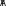
\includegraphics[width=0.45\textwidth,height=\textheight]{week4/week4_files/figure-pdf/unnamed-chunk-3-1.pdf}

}

\end{figure}

\begin{Shaded}
\begin{Highlighting}[]
\FunctionTok{qqnorm}\NormalTok{(x)}
\FunctionTok{abline}\NormalTok{(}\AttributeTok{a =} \DecValTok{0}\NormalTok{, }\AttributeTok{b =} \DecValTok{1}\NormalTok{)}
\end{Highlighting}
\end{Shaded}

\begin{figure}[H]

{\centering \includegraphics[width=0.45\textwidth,height=\textheight]{week4/week4_files/figure-pdf/unnamed-chunk-3-2.pdf}

}

\end{figure}

\begin{Shaded}
\begin{Highlighting}[]
\NormalTok{x }\OtherTok{\textless{}{-}} \FunctionTok{rcauchy}\NormalTok{(}\AttributeTok{n =} \DecValTok{1000}\NormalTok{)}
\FunctionTok{hist}\NormalTok{(x, }\AttributeTok{breaks =} \DecValTok{100}\NormalTok{)}
\end{Highlighting}
\end{Shaded}

\begin{figure}[H]

{\centering \includegraphics[width=0.45\textwidth,height=\textheight]{week4/week4_files/figure-pdf/unnamed-chunk-3-3.pdf}

}

\end{figure}

\begin{Shaded}
\begin{Highlighting}[]
\FunctionTok{qqnorm}\NormalTok{(x)}
\FunctionTok{abline}\NormalTok{(}\AttributeTok{a =} \DecValTok{0}\NormalTok{, }\AttributeTok{b =} \DecValTok{1}\NormalTok{)}
\end{Highlighting}
\end{Shaded}

\begin{figure}[H]

{\centering \includegraphics[width=0.45\textwidth,height=\textheight]{week4/week4_files/figure-pdf/unnamed-chunk-3-4.pdf}

}

\end{figure}

\begin{Shaded}
\begin{Highlighting}[]
\NormalTok{x }\OtherTok{\textless{}{-}} \FunctionTok{rlnorm}\NormalTok{(}\AttributeTok{n =} \DecValTok{1000}\NormalTok{, }\AttributeTok{meanlog =} \FloatTok{2.5}\NormalTok{, }\AttributeTok{sdlog =}\NormalTok{ .}\DecValTok{1}\NormalTok{)}
\NormalTok{x }\OtherTok{\textless{}{-}}\NormalTok{ x }\SpecialCharTok{{-}} \FunctionTok{mean}\NormalTok{(x)}
\FunctionTok{hist}\NormalTok{(x, }\AttributeTok{breaks =} \DecValTok{100}\NormalTok{)}
\end{Highlighting}
\end{Shaded}

\begin{figure}[H]

{\centering \includegraphics[width=0.45\textwidth,height=\textheight]{week4/week4_files/figure-pdf/unnamed-chunk-3-5.pdf}

}

\end{figure}

\begin{Shaded}
\begin{Highlighting}[]
\FunctionTok{qqnorm}\NormalTok{(x)}
\FunctionTok{abline}\NormalTok{(}\AttributeTok{a =} \DecValTok{0}\NormalTok{, }\AttributeTok{b =} \DecValTok{1}\NormalTok{)}
\end{Highlighting}
\end{Shaded}

\begin{figure}[H]

{\centering \includegraphics[width=0.45\textwidth,height=\textheight]{week4/week4_files/figure-pdf/unnamed-chunk-3-6.pdf}

}

\end{figure}

Check out the \texttt{ggResidpanel} and \texttt{olsrr} packages!

\hypertarget{transformations-of-the-outcome}{%
\subsection{Transformations of the
Outcome}\label{transformations-of-the-outcome}}

Transforming the outcome is often a successful way to reduce the
skewness of the residuals.

The idea is that often large values of the outcome yield the largest
residuals.

Pulling these values back towards the center will yield a more symmetric
distribution.

A popular transformation is to replace \(Y\) with \(\log (Y)\) where
\(\log = \ln\)).

Other ``power transformations'' that are often effective are \(Y^k\)
with smaller values of \(k\) pulling in the right tail more strongly.

\begin{Shaded}
\begin{Highlighting}[]
\FunctionTok{hist}\NormalTok{(hers}\SpecialCharTok{$}\NormalTok{LDL)}
\end{Highlighting}
\end{Shaded}

\begin{figure}[H]

{\centering \includegraphics{week4/week4_files/figure-pdf/unnamed-chunk-4-1.pdf}

}

\end{figure}

\begin{Shaded}
\begin{Highlighting}[]
\FunctionTok{plot}\NormalTok{(}\FunctionTok{lm}\NormalTok{(}\AttributeTok{data =}\NormalTok{ hers, LDL }\SpecialCharTok{\textasciitilde{}}\NormalTok{ BMI), }\AttributeTok{which =} \DecValTok{2}\NormalTok{)}
\end{Highlighting}
\end{Shaded}

\begin{figure}[H]

{\centering \includegraphics{week4/week4_files/figure-pdf/unnamed-chunk-4-2.pdf}

}

\end{figure}

\begin{Shaded}
\begin{Highlighting}[]
\FunctionTok{plot}\NormalTok{(}\FunctionTok{lm}\NormalTok{(}\AttributeTok{data =}\NormalTok{ hers, }\FunctionTok{log}\NormalTok{(LDL) }\SpecialCharTok{\textasciitilde{}}\NormalTok{ BMI), }\AttributeTok{which =} \DecValTok{2}\NormalTok{)}
\end{Highlighting}
\end{Shaded}

\begin{figure}[H]

{\centering \includegraphics{week4/week4_files/figure-pdf/unnamed-chunk-4-3.pdf}

}

\end{figure}

These changes alter the interpretation of the model coefficients.

\[\log(Y_i) = \beta_0 + \beta_1 x_i + \varepsilon_i\]

\[\Longrightarrow Y_i = \exp(\beta_0) \exp(\beta_1 x_i) \exp(\varepsilon_i)\]

Here, \(\exp(\beta_1)\) is the ratio of the expected value of \(y\)
corresponding to a one-unit increase in \(x\). To see this note that

\[\frac{\mathbb E(Y_i | x_i = x^*+1)}{\mathbb E(Y_i | x_i = x^*)} = \frac{exp(\beta_0)\exp(\beta_1(x^*+1)) \mathbb E[\exp(\varepsilon_i)]}{\exp(\beta_0)\exp(\beta_1 x^*) \mathbb E[\exp(\varepsilon_i)]}\]

\[ = \frac{\exp(\beta_1x^* + \beta_1)}{\exp(\beta_1 x^*)} = exp(\beta_1)\]

People often report \(100(e^{\hat \beta_1} - 1)\) as the percent change
in \(\mathbb E(Y_i)\) per unit increase in \(x\).

\hypertarget{assessing-constant-variance}{%
\section{Assessing Constant
Variance}\label{assessing-constant-variance}}

Standard multiple linear regression assumes constant variance, or
{homoscedasticity}:

\[\sigma^2 = \text{Var}(\varepsilon_i) = \text{Var}(Y_i | x_i)\]

When the errors are heteroscedastic, this can invalidate inference in
both small and large samples.

We can plot \(e_i\) vs.~\(\hat y_i\) and look for changes in variance of
\(e_i\) to get a sense of whether homoscedasticity holds.

\begin{itemize}
\tightlist
\item
  Some people prefer to use the studentized residuals for this since
  technically \(\text{Var}(e_i) = \sigma^2(1-h_i)\).
\item
  As we will see later, \(h_i\) is small for most observations in the
  sample so in practice many argue this makes little difference.
\end{itemize}

\begin{Shaded}
\begin{Highlighting}[]
\NormalTok{lm.ldl }\OtherTok{\textless{}{-}} \FunctionTok{lm}\NormalTok{(LDL }\SpecialCharTok{\textasciitilde{}}\NormalTok{ BMI, }\AttributeTok{data =}\NormalTok{ hers)}

\FunctionTok{plot}\NormalTok{(}\FunctionTok{residuals}\NormalTok{(lm.ldl), }\AttributeTok{main =} \StringTok{"Satisfactory Residual Plot"}\NormalTok{)}
\end{Highlighting}
\end{Shaded}

\begin{figure}[H]

{\centering \includegraphics{week4/week4_files/figure-pdf/unnamed-chunk-5-1.pdf}

}

\end{figure}

\begin{Shaded}
\begin{Highlighting}[]
\NormalTok{df }\OtherTok{\textless{}{-}}\NormalTok{ tibble}\SpecialCharTok{::}\FunctionTok{tibble}\NormalTok{(}
  \AttributeTok{x =} \FunctionTok{runif}\NormalTok{(}\DecValTok{1000}\NormalTok{, }\AttributeTok{min =} \DecValTok{0}\NormalTok{, }\AttributeTok{max =} \DecValTok{10}\NormalTok{),}
  \AttributeTok{y =} \FunctionTok{rnorm}\NormalTok{(}\AttributeTok{n =} \DecValTok{1000}\NormalTok{, }\AttributeTok{sd =} \FunctionTok{sqrt}\NormalTok{(x)))}

\FunctionTok{plot}\NormalTok{(df}\SpecialCharTok{$}\NormalTok{x, }\FunctionTok{residuals}\NormalTok{(}\FunctionTok{lm}\NormalTok{(}\AttributeTok{data =}\NormalTok{ df, y }\SpecialCharTok{\textasciitilde{}}\NormalTok{ x)), }\AttributeTok{main =} \StringTok{"Unsatisfactory Residual Plot"}\NormalTok{)}
\end{Highlighting}
\end{Shaded}

\begin{figure}[H]

{\centering \includegraphics{week4/week4_files/figure-pdf/unnamed-chunk-5-2.pdf}

}

\end{figure}

\hypertarget{assessing-linearity}{%
\section{Assessing Linearity}\label{assessing-linearity}}

Unless we add non-linear terms, linear regression assumes the functional
form relating the mean of \(Y\) to \(x\) is a straight line. Violations
to this assumption may occur for a variety of reasons including:

\begin{itemize}
\tightlist
\item
  ceiling or floor effects
\item
  U or inverse-U shaped relationships (e.g., manganese is both a
  nutrient and toxin)
\end{itemize}

\begin{figure}

{\centering \includegraphics[width=0.5\textwidth,height=\textheight]{week4/images/manganese.jpeg}

}

\end{figure}

Claus Henn B, Ettinger AS, Schwartz J, Téllez-Rojo MM, Lamadrid-Figueroa
H, Hernández-Avila M, Schnaas L, Amarasiriwardena C, Bellinger DC, Hu H,
Wright RO. Early postnatal blood manganese levels and children's
neurodevelopment. Epidemiology. 2010 Jul;21(4):433-9. doi:
10.1097/ede.0b013e3181df8e52. PMID: 20549838; PMCID: PMC3127440.

\url{https://pubmed.ncbi.nlm.nih.gov/20549838/}

\begin{Shaded}
\begin{Highlighting}[]
\NormalTok{df }\OtherTok{\textless{}{-}}\NormalTok{ tibble}\SpecialCharTok{::}\FunctionTok{tibble}\NormalTok{(}
  \AttributeTok{x =} \FunctionTok{runif}\NormalTok{(}\AttributeTok{n =} \DecValTok{1000}\NormalTok{, }\AttributeTok{min =} \SpecialCharTok{{-}}\DecValTok{5}\NormalTok{, }\AttributeTok{max =} \DecValTok{10}\NormalTok{),}
  \AttributeTok{y =}\NormalTok{ x}\SpecialCharTok{\^{}}\DecValTok{2} \SpecialCharTok{+} \DecValTok{3}\SpecialCharTok{*}\NormalTok{x }\SpecialCharTok{+} \FunctionTok{exp}\NormalTok{(x}\SpecialCharTok{/}\DecValTok{10}\NormalTok{) }\SpecialCharTok{+} \FunctionTok{rnorm}\NormalTok{(}\AttributeTok{n =} \DecValTok{1000}\NormalTok{, }\AttributeTok{sd =} \DecValTok{10}\NormalTok{))}

\FunctionTok{plot}\NormalTok{(df}\SpecialCharTok{$}\NormalTok{x, df}\SpecialCharTok{$}\NormalTok{y, }\AttributeTok{main =} \StringTok{"data with nonlinear pattern"}\NormalTok{)}
\end{Highlighting}
\end{Shaded}

\begin{figure}[H]

{\centering \includegraphics{week4/week4_files/figure-pdf/unnamed-chunk-7-1.pdf}

}

\end{figure}

\begin{Shaded}
\begin{Highlighting}[]
\FunctionTok{plot}\NormalTok{(df}\SpecialCharTok{$}\NormalTok{x, }\FunctionTok{residuals}\NormalTok{(}\FunctionTok{lm}\NormalTok{(y}\SpecialCharTok{\textasciitilde{}}\NormalTok{x, df)), }\AttributeTok{main =} \StringTok{"nonlinear residuals"}\NormalTok{)}
\end{Highlighting}
\end{Shaded}

\begin{figure}[H]

{\centering \includegraphics{week4/week4_files/figure-pdf/unnamed-chunk-7-2.pdf}

}

\end{figure}

\begin{Shaded}
\begin{Highlighting}[]
\NormalTok{hers.sample }\OtherTok{\textless{}{-}} \FunctionTok{na.omit}\NormalTok{(hers[,}\FunctionTok{c}\NormalTok{(}\StringTok{"HDL"}\NormalTok{, }\StringTok{"BMI"}\NormalTok{)]) }\SpecialCharTok{|\textgreater{}} 
\NormalTok{  dplyr}\SpecialCharTok{::}\FunctionTok{sample\_frac}\NormalTok{(.}\DecValTok{1}\NormalTok{)}
\NormalTok{lm.hdl.bmi }\OtherTok{\textless{}{-}} \FunctionTok{lm}\NormalTok{(HDL }\SpecialCharTok{\textasciitilde{}}\NormalTok{ BMI, }\AttributeTok{data =}\NormalTok{ hers.sample)}

\FunctionTok{plot}\NormalTok{(hers.sample}\SpecialCharTok{$}\NormalTok{BMI, }\FunctionTok{residuals}\NormalTok{(lm.hdl.bmi))}

\FunctionTok{lines}\NormalTok{(}\FunctionTok{lowess}\NormalTok{(lm.hdl.bmi}\SpecialCharTok{$}\NormalTok{residuals}\SpecialCharTok{\textasciitilde{}}\NormalTok{hers.sample}\SpecialCharTok{$}\NormalTok{BMI))}
\end{Highlighting}
\end{Shaded}

\begin{figure}[H]

{\centering \includegraphics{week4/week4_files/figure-pdf/unnamed-chunk-8-1.pdf}

}

\end{figure}

\hypertarget{assessing-linearity-in-multiple-linear-regression}{%
\subsection{Assessing Linearity in Multiple Linear
Regression}\label{assessing-linearity-in-multiple-linear-regression}}

In multiple linear regression, we want to assess whether it's
appropriate to assume linearity between a given \(x_j\) and \(Y\) *after
conditioning on all the \(x_{-j}\).

Neither scatterplots of \(Y\) vs.~\(x_j\) nor scatterplots of \(e\)
vs.~\(x_j\) allow us to appropriately evaluate this.

{Partial regression plots} are a tool that allow us to assess the form
of the relationship between \(x_j\) and \(Y\) after conditioning on all
the \(x_{-j}\). They are:

\begin{itemize}
\tightlist
\item
  A variation of the plot of residuals vs.~predictors.
\item
  Also called ``added variable plots'' or ``adjusted variable plots''.
\end{itemize}

Consider the candidate model

\[y_i = \beta_0 + \beta_1 x_{i1} + \beta_2 x_{i2} + \beta_3 x_{i3} + \varepsilon_i\]

and we want to assess whether it is reasonable to assume linearity
between \(x_1\) and \(Y\), conditional on \(x_2\) and \(x_3\).

To create a partial regression plot, we

\begin{enumerate}
\def\labelenumi{\arabic{enumi}.}
\tightlist
\item
  Regress \(y\) on only \(x_2,\) \(x_3\) and obtain the residuals
  \(e_i(y|x_2,x_3)\). * What's leftover in \(Y\) after conditioning
  \(Y\) after conditioning on \(x_2, x_3\).
\item
  Regress \(x_1\) on \(x_2, x_3\) and obtain the residuals
  \(e_i(x_1|x_2,x_3)\) * What's leftover in \(x_1\) after conditioning
  \(x_2, x_3\)
\item
  Plot \(e_i(y|x_2,x_3)\) against \(e_i(x_1|x_2,x_3)\) and look for any
  nonlinearity * This is the association between what's leftover in
  \(Y\) and \(x_1\) after accounting for \(x_2,x_3\).
\end{enumerate}

\begin{Shaded}
\begin{Highlighting}[]
\CommentTok{\# we can use car::av.plots(lm.hdl.bmi)}
\NormalTok{lm.ldl.bmi.age }\OtherTok{\textless{}{-}} \FunctionTok{lm}\NormalTok{(HDL }\SpecialCharTok{\textasciitilde{}}\NormalTok{ BMI }\SpecialCharTok{+}\NormalTok{ age, }\AttributeTok{data =}\NormalTok{ hers)}
\NormalTok{car}\SpecialCharTok{::}\FunctionTok{avPlots}\NormalTok{(lm.ldl.bmi.age, }\AttributeTok{main =} \FunctionTok{expression}\NormalTok{(}\FunctionTok{paste}\NormalTok{(}\StringTok{"Partial Regression Plot for E(HDL) = "}\NormalTok{, beta[}\DecValTok{0}\NormalTok{] }\SpecialCharTok{+}\NormalTok{ beta[}\DecValTok{1}\NormalTok{], }\StringTok{"BMI + "}\NormalTok{, beta[}\DecValTok{2}\NormalTok{], }\StringTok{"Age"}\NormalTok{)))}
\end{Highlighting}
\end{Shaded}

\begin{figure}[H]

{\centering \includegraphics{week4/week4_files/figure-pdf/unnamed-chunk-9-1.pdf}

}

\end{figure}

Perks of partial regression plots:

\begin{itemize}
\tightlist
\item
  If we fit a linear model to the data in the plot for \(x_j\), the
  slope estimate would be exactly the same as the estimated linear
  coefficient for \(x_j\) in the full model of \(Y\) (conditional on all
  variables)
\item
  This tells us that the plots are visualizing the same relationships
  that are being quantified in the full model
\end{itemize}

Caveats of partial regression plots

\begin{itemize}
\tightlist
\item
  Can't detect interactions between regressors.
\item
  The presence of strong multicollinearity can cause partial regression
  plots to be misleading.
\end{itemize}

\hypertarget{remedial-measures-for-non-linearity}{%
\subsubsection{Remedial measures for
non-linearity}\label{remedial-measures-for-non-linearity}}

Could include polynomial terms, but these can behave erratically,
particularly in the tails of the distribution.

Modern approaches and advice are to use splines or generalized (GAMs) to
capture non-linearity.

Splines and GAMs can still be unreliable in regions of the predictor
space with little data, but are generally more stable than polynomial
models.

Won't cover them here, but they can be easily operationalized within the
linear model framework.

Usually need to visualize associations since we're no longer fitting
straight lines with a constant slope.

\hypertarget{outliers-and-influential-points}{%
\section{Outliers and Influential
Points}\label{outliers-and-influential-points}}

Outlying observations with large residuals can have a disproportionately
large effect on regression results.

We want to make sure regression results are not driven by only a few
points.

These influential points could:

\begin{itemize}
\tightlist
\item
  Cause associations between an \(x\) and \(Y\) that \emph{would be
  clearly} significant with their inclusion to become non-significant.
\item
  Cause associations that \emph{would clearly not be} significant
  without their inclusion to become significant.
\end{itemize}

If results are significantly impacted by the inclusion or exclusion of a
small subset of points, \emph{this should be reported}. Usually one
should report results both with and without those influential points.

Possible explanations for outliers include:

\begin{itemize}
\tightlist
\item
  ``Bad'' data that results from an explainable (or unexplained) event
  (e.g., misrecorded measurement, instrument malfunction, etc.). Only in
  the case when data are corrupted due to an \emph{explained event}
  should one discard the observation. In the ideal case (unrealistic as
  it is), one would go back and try to retrieve the original data.
\item
  Inadequacies in the model. In this case, we would not want to exclude
  observations in any effort to make the data ``agree overall with the
  model''.
\item
  Poor sampling of observations in the tail of the distribution --- the
  data generating process may actually be long-tailed!
\end{itemize}

It tends to be the case that large \(x\)-outliers have much more
influence (or leverage) than \(y\)-outliers.

We'll use the terminology {influential points} for terms we've confirmed
have high influence on a given regression. Otherwise we'll use the terms
{high leverage points} or {outliers} for points that are unique in some
regards but unconfirmed as having large influence on our model.

\begin{Shaded}
\begin{Highlighting}[]
\CommentTok{\# dataset with a low{-}influence outlier point }
\NormalTok{df }\OtherTok{\textless{}{-}}\NormalTok{ tibble}\SpecialCharTok{::}\FunctionTok{tibble}\NormalTok{(}
  \AttributeTok{x =} \FunctionTok{rnorm}\NormalTok{(}\AttributeTok{n =} \DecValTok{1000}\NormalTok{),}
  \AttributeTok{y =}\NormalTok{ x}\SpecialCharTok{*}\NormalTok{.}\DecValTok{25} \SpecialCharTok{+} \FunctionTok{rnorm}\NormalTok{(}\AttributeTok{n =} \DecValTok{1000}\NormalTok{, }\AttributeTok{sd =}\NormalTok{ .}\DecValTok{5}\NormalTok{))}

\NormalTok{df2 }\OtherTok{\textless{}{-}} \FunctionTok{bind\_rows}\NormalTok{(df, }\FunctionTok{c}\NormalTok{(}\AttributeTok{x =} \DecValTok{0}\NormalTok{, }\AttributeTok{y =} \DecValTok{10}\NormalTok{))}

\NormalTok{lm1 }\OtherTok{\textless{}{-}} \FunctionTok{lm}\NormalTok{(y }\SpecialCharTok{\textasciitilde{}}\NormalTok{ x, }\AttributeTok{data =}\NormalTok{ df)}
\NormalTok{lm2 }\OtherTok{\textless{}{-}} \FunctionTok{lm}\NormalTok{(y }\SpecialCharTok{\textasciitilde{}}\NormalTok{ x, }\AttributeTok{data =}\NormalTok{ df2)}

\FunctionTok{ggplot}\NormalTok{(df2, }\FunctionTok{aes}\NormalTok{(}\AttributeTok{x =}\NormalTok{ x, }\AttributeTok{y =}\NormalTok{ y)) }\SpecialCharTok{+} 
  \FunctionTok{geom\_point}\NormalTok{(}\AttributeTok{alpha =}\NormalTok{ .}\DecValTok{15}\NormalTok{, }\AttributeTok{size =} \DecValTok{2}\NormalTok{) }\SpecialCharTok{+} 
  \FunctionTok{geom\_abline}\NormalTok{(}
    \AttributeTok{mapping =} \FunctionTok{aes}\NormalTok{(}
      \AttributeTok{color =} \StringTok{\textquotesingle{}w/o outlier\textquotesingle{}}\NormalTok{,}
      \AttributeTok{linetype =} \StringTok{\textquotesingle{}w/o outlier\textquotesingle{}}\NormalTok{,}
      \AttributeTok{intercept =} \FunctionTok{coef}\NormalTok{(lm1)[}\DecValTok{1}\NormalTok{],}
      \AttributeTok{slope =} \FunctionTok{coef}\NormalTok{(lm1)[}\DecValTok{2}\NormalTok{]}
\NormalTok{    ),}
    \AttributeTok{size =} \DecValTok{2}
\NormalTok{  ) }\SpecialCharTok{+}
  \FunctionTok{geom\_point}\NormalTok{(}\FunctionTok{aes}\NormalTok{(}\AttributeTok{x =} \DecValTok{0}\NormalTok{, }\AttributeTok{y =} \DecValTok{10}\NormalTok{, }\AttributeTok{shape =} \StringTok{\textquotesingle{}low{-}influence outlier\textquotesingle{}}\NormalTok{), }\AttributeTok{size =} \DecValTok{2}\NormalTok{, }\AttributeTok{color =} \StringTok{\textquotesingle{}red\textquotesingle{}}\NormalTok{, }\AttributeTok{alpha =}\NormalTok{ .}\DecValTok{5}\NormalTok{) }\SpecialCharTok{+} 
  \FunctionTok{geom\_abline}\NormalTok{(}
    \AttributeTok{mapping =} \FunctionTok{aes}\NormalTok{(}
      \AttributeTok{color =} \StringTok{\textquotesingle{}with outlier\textquotesingle{}}\NormalTok{,}
      \AttributeTok{linetype =} \StringTok{\textquotesingle{}with outlier\textquotesingle{}}\NormalTok{,}
      \AttributeTok{intercept =} \FunctionTok{coef}\NormalTok{(lm2)[}\DecValTok{1}\NormalTok{],}
      \AttributeTok{slope =} \FunctionTok{coef}\NormalTok{(lm2)[}\DecValTok{2}\NormalTok{]}
\NormalTok{    ),}
    \AttributeTok{size =} \FloatTok{1.75}
\NormalTok{  ) }\SpecialCharTok{+}
  \FunctionTok{scale\_color\_manual}\NormalTok{(}\AttributeTok{values =} \FunctionTok{c}\NormalTok{(}
    \StringTok{\textquotesingle{}w/o outlier\textquotesingle{}} \OtherTok{=} \StringTok{\textquotesingle{}cornflowerblue\textquotesingle{}}\NormalTok{,}
    \StringTok{\textquotesingle{}with outlier\textquotesingle{}} \OtherTok{=} \StringTok{\textquotesingle{}orange\textquotesingle{}}
\NormalTok{  )) }\SpecialCharTok{+}
  \FunctionTok{scale\_linetype\_manual}\NormalTok{(}\AttributeTok{values =} \FunctionTok{c}\NormalTok{(}\StringTok{\textquotesingle{}w/o outlier\textquotesingle{}} \OtherTok{=} \StringTok{\textquotesingle{}solid\textquotesingle{}}\NormalTok{,}
                                   \StringTok{\textquotesingle{}with outlier\textquotesingle{}} \OtherTok{=} \StringTok{\textquotesingle{}dashed\textquotesingle{}}\NormalTok{)) }\SpecialCharTok{+} 
  \FunctionTok{labs}\NormalTok{(}\AttributeTok{color =} \StringTok{\textquotesingle{}model type\textquotesingle{}}\NormalTok{, }\AttributeTok{linetype =} \StringTok{\textquotesingle{}model type\textquotesingle{}}\NormalTok{) }\SpecialCharTok{+} 
  \FunctionTok{theme\_bw}\NormalTok{() }\SpecialCharTok{+} 
  \FunctionTok{scale\_shape\_manual}\NormalTok{(}\AttributeTok{values =} \FunctionTok{c}\NormalTok{(}\StringTok{\textquotesingle{}low{-}influence outlier\textquotesingle{}} \OtherTok{=} \DecValTok{2}\NormalTok{)) }\SpecialCharTok{+} 
  \FunctionTok{ggtitle}\NormalTok{(}\StringTok{"Comparing Models with and without the Influential Point"}\NormalTok{)}
\end{Highlighting}
\end{Shaded}

\begin{verbatim}
Warning: Using `size` aesthetic for lines was deprecated in ggplot2 3.4.0.
i Please use `linewidth` instead.
\end{verbatim}

\begin{figure}[H]

{\centering \includegraphics{week4/week4_files/figure-pdf/unnamed-chunk-10-1.pdf}

}

\end{figure}

\begin{Shaded}
\begin{Highlighting}[]
\CommentTok{\# dataset with a high{-}influence outlier point }
\NormalTok{df }\OtherTok{\textless{}{-}}\NormalTok{ tibble}\SpecialCharTok{::}\FunctionTok{tibble}\NormalTok{(}
  \AttributeTok{x =} \FunctionTok{rnorm}\NormalTok{(}\AttributeTok{n =} \DecValTok{100}\NormalTok{),}
  \AttributeTok{y =}\NormalTok{ x}\SpecialCharTok{*}\NormalTok{.}\DecValTok{25} \SpecialCharTok{+} \FunctionTok{rnorm}\NormalTok{(}\AttributeTok{n =} \DecValTok{100}\NormalTok{, }\AttributeTok{sd =}\NormalTok{ .}\DecValTok{5}\NormalTok{))}

\NormalTok{df2 }\OtherTok{\textless{}{-}} \FunctionTok{bind\_rows}\NormalTok{(df, }\FunctionTok{c}\NormalTok{(}\AttributeTok{x =} \DecValTok{7}\NormalTok{, }\AttributeTok{y =} \SpecialCharTok{{-}}\DecValTok{1}\NormalTok{))}

\NormalTok{lm1 }\OtherTok{\textless{}{-}} \FunctionTok{lm}\NormalTok{(y }\SpecialCharTok{\textasciitilde{}}\NormalTok{ x, }\AttributeTok{data =}\NormalTok{ df)}
\NormalTok{lm2 }\OtherTok{\textless{}{-}} \FunctionTok{lm}\NormalTok{(y }\SpecialCharTok{\textasciitilde{}}\NormalTok{ x, }\AttributeTok{data =}\NormalTok{ df2)}

\FunctionTok{ggplot}\NormalTok{(df2, }\FunctionTok{aes}\NormalTok{(}\AttributeTok{x =}\NormalTok{ x, }\AttributeTok{y =}\NormalTok{ y)) }\SpecialCharTok{+} 
  \FunctionTok{geom\_point}\NormalTok{(}\AttributeTok{alpha =}\NormalTok{ .}\DecValTok{25}\NormalTok{, }\AttributeTok{size =} \DecValTok{2}\NormalTok{) }\SpecialCharTok{+} 
  \FunctionTok{geom\_abline}\NormalTok{(}
    \AttributeTok{mapping =} \FunctionTok{aes}\NormalTok{(}
      \AttributeTok{color =} \StringTok{\textquotesingle{}w/o outlier\textquotesingle{}}\NormalTok{,}
      \AttributeTok{linetype =} \StringTok{\textquotesingle{}w/o outlier\textquotesingle{}}\NormalTok{,}
      \AttributeTok{intercept =} \FunctionTok{coef}\NormalTok{(lm1)[}\DecValTok{1}\NormalTok{],}
      \AttributeTok{slope =} \FunctionTok{coef}\NormalTok{(lm1)[}\DecValTok{2}\NormalTok{]}
\NormalTok{    ),}
    \AttributeTok{size =} \DecValTok{2}
\NormalTok{  ) }\SpecialCharTok{+}
  \FunctionTok{geom\_point}\NormalTok{(}\FunctionTok{aes}\NormalTok{(}\AttributeTok{x =} \DecValTok{7}\NormalTok{, }\AttributeTok{y =} \SpecialCharTok{{-}}\DecValTok{1}\NormalTok{, }\AttributeTok{shape =} \StringTok{\textquotesingle{}influential point\textquotesingle{}}\NormalTok{), }\AttributeTok{size =} \DecValTok{2}\NormalTok{, }\AttributeTok{color =} \StringTok{\textquotesingle{}red\textquotesingle{}}\NormalTok{, }\AttributeTok{alpha =}\NormalTok{ .}\DecValTok{5}\NormalTok{) }\SpecialCharTok{+} 
  \FunctionTok{geom\_abline}\NormalTok{(}
    \AttributeTok{mapping =} \FunctionTok{aes}\NormalTok{(}
      \AttributeTok{color =} \StringTok{\textquotesingle{}with outlier\textquotesingle{}}\NormalTok{,}
      \AttributeTok{linetype =} \StringTok{\textquotesingle{}with outlier\textquotesingle{}}\NormalTok{,}
      \AttributeTok{intercept =} \FunctionTok{coef}\NormalTok{(lm2)[}\DecValTok{1}\NormalTok{],}
      \AttributeTok{slope =} \FunctionTok{coef}\NormalTok{(lm2)[}\DecValTok{2}\NormalTok{]}
\NormalTok{    ),}
    \AttributeTok{size =} \FloatTok{1.75}
\NormalTok{  ) }\SpecialCharTok{+}
  \FunctionTok{scale\_color\_manual}\NormalTok{(}\AttributeTok{values =} \FunctionTok{c}\NormalTok{(}
    \StringTok{\textquotesingle{}w/o outlier\textquotesingle{}} \OtherTok{=} \StringTok{\textquotesingle{}cornflowerblue\textquotesingle{}}\NormalTok{,}
    \StringTok{\textquotesingle{}with outlier\textquotesingle{}} \OtherTok{=} \StringTok{\textquotesingle{}orange\textquotesingle{}}
\NormalTok{  )) }\SpecialCharTok{+}
  \FunctionTok{scale\_linetype\_manual}\NormalTok{(}\AttributeTok{values =} \FunctionTok{c}\NormalTok{(}\StringTok{\textquotesingle{}w/o outlier\textquotesingle{}} \OtherTok{=} \StringTok{\textquotesingle{}solid\textquotesingle{}}\NormalTok{,}
                                   \StringTok{\textquotesingle{}with outlier\textquotesingle{}} \OtherTok{=} \StringTok{\textquotesingle{}dashed\textquotesingle{}}\NormalTok{)) }\SpecialCharTok{+} 
  \FunctionTok{labs}\NormalTok{(}\AttributeTok{color =} \StringTok{\textquotesingle{}model type\textquotesingle{}}\NormalTok{, }\AttributeTok{linetype =} \StringTok{\textquotesingle{}model type\textquotesingle{}}\NormalTok{) }\SpecialCharTok{+} 
  \FunctionTok{theme\_bw}\NormalTok{() }\SpecialCharTok{+} 
  \FunctionTok{scale\_shape\_manual}\NormalTok{(}\AttributeTok{values =} \FunctionTok{c}\NormalTok{(}\StringTok{\textquotesingle{}influential point\textquotesingle{}} \OtherTok{=} \DecValTok{2}\NormalTok{)) }\SpecialCharTok{+} 
  \FunctionTok{ggtitle}\NormalTok{(}\StringTok{"Comparing Models with and without the Influential Point"}\NormalTok{)}
\end{Highlighting}
\end{Shaded}

\begin{figure}[H]

{\centering \includegraphics{week4/week4_files/figure-pdf/unnamed-chunk-10-2.pdf}

}

\end{figure}

\hypertarget{quantifying-measure-of-leverage}{%
\subsection{Quantifying Measure of
Leverage}\label{quantifying-measure-of-leverage}}

\(h_i\) (\(i\)th diagonal element of \(H\)) is known as the {leverage}
of observation \(i\).

\(h_i\) is a measure of \(x_i\)'s distance from the center in the
\(x\)-dimension. E.g., in SLR:

\[h_i = \frac{1}{n} + \frac{(x_i - \bar x)^2}{\sum_{i=1}^n (x_i - \bar x)^2}\]

\(h_i\) is also the weight given to the observed outcome for unit \(i\)
when computing its own fitted value.

Since \(\hat y = Hy\),

\[\hat y_i = H_i y = h_{i1}y_1 + h_{i2} y_2 + \cdots + h_{ii}y_i + \cdots + h_{in}y_n\]

where \(H_i\) is the \(i\)th row of \(H\).

This is saying that units whose \(x_i\) is further from the mean tend to
have the most influence on model fit/fitted values. The average value of
\(h_i\) is \(\bar h = (p+1)/n\) over all \(i = 1, ..., n\).

A rule of thumb can be to classify observation \(i\) as a high leverage
point if \[h_i > 2 \times \bar h = 2 (p+1)/n.\]

\begin{Shaded}
\begin{Highlighting}[]
\NormalTok{leverage }\OtherTok{\textless{}{-}} \FunctionTok{hat}\NormalTok{(}\FunctionTok{model.matrix}\NormalTok{(}\FunctionTok{lm}\NormalTok{(SBP }\SpecialCharTok{\textasciitilde{}}\NormalTok{ age, hers }\SpecialCharTok{|\textgreater{}}\NormalTok{ dplyr}\SpecialCharTok{::}\FunctionTok{sample\_frac}\NormalTok{(.}\DecValTok{1}\NormalTok{))))}
\FunctionTok{plot}\NormalTok{(leverage, }\AttributeTok{main =} \FunctionTok{expression}\NormalTok{(}\FunctionTok{paste}\NormalTok{(}\StringTok{"Leverage "}\NormalTok{, h[i], }\StringTok{" values and its rule of thumb threshold"}\NormalTok{)))}
\FunctionTok{abline}\NormalTok{(}\AttributeTok{a =} \DecValTok{2} \SpecialCharTok{*} \FunctionTok{mean}\NormalTok{(leverage), }\AttributeTok{b =} \DecValTok{0}\NormalTok{)}
\end{Highlighting}
\end{Shaded}

\begin{figure}[H]

{\centering \includegraphics{week4/week4_files/figure-pdf/unnamed-chunk-11-1.pdf}

}

\end{figure}

\hypertarget{studentized-residuals-1}{%
\subsubsection{Studentized Residuals}\label{studentized-residuals-1}}

In order to quantify \(y\)-outliers, one might use studentized
residuals.

Recall that if the model is correct, the studentized residuals are

\[r_i = \frac{e_i}{\sqrt{\widehat{\text{Var}} (e_i) }}\] should behave
as \(\mathcal N(0,1)\) random variables and hence have constant
variance. If the model is correct, we would expect \(-3 < r_i < 3\).
Thus a residual satisfying \(|r_i| > 3\) warrants attention.

\begin{Shaded}
\begin{Highlighting}[]
\NormalTok{hers.ldl.bmi.complete }\OtherTok{\textless{}{-}}\NormalTok{ hers }\SpecialCharTok{|\textgreater{}} \FunctionTok{select}\NormalTok{(LDL, BMI) }\SpecialCharTok{|\textgreater{}} \FunctionTok{na.omit}\NormalTok{() }\SpecialCharTok{|\textgreater{}}\NormalTok{ dplyr}\SpecialCharTok{::}\FunctionTok{sample\_frac}\NormalTok{(.}\DecValTok{1}\NormalTok{)}
\NormalTok{stud.resid }\OtherTok{\textless{}{-}} \FunctionTok{rstandard}\NormalTok{(}\FunctionTok{lm}\NormalTok{(LDL}\SpecialCharTok{\textasciitilde{}}\NormalTok{BMI, hers.ldl.bmi.complete))}
\FunctionTok{plot}\NormalTok{(hers.ldl.bmi.complete}\SpecialCharTok{$}\NormalTok{BMI,stud.resid, }\AttributeTok{ylab=}\StringTok{"Studentized Residuals"}\NormalTok{,}
  \AttributeTok{main=}\StringTok{"log(LDL) \textasciitilde{} BMI"}\NormalTok{, }\AttributeTok{ylim=}\FunctionTok{c}\NormalTok{(}\SpecialCharTok{{-}}\FloatTok{3.5}\NormalTok{,}\FloatTok{3.5}\NormalTok{))}
\FunctionTok{abline}\NormalTok{(}\AttributeTok{h=}\DecValTok{3}\NormalTok{, }\AttributeTok{lty=}\DecValTok{3}\NormalTok{)}
\FunctionTok{abline}\NormalTok{(}\AttributeTok{h=}\SpecialCharTok{{-}}\DecValTok{3}\NormalTok{,}\AttributeTok{lty=}\DecValTok{3}\NormalTok{)}
\end{Highlighting}
\end{Shaded}

\begin{figure}[H]

{\centering \includegraphics{week4/week4_files/figure-pdf/unnamed-chunk-12-1.pdf}

}

\end{figure}

\begin{Shaded}
\begin{Highlighting}[]
\NormalTok{stud.resid }\OtherTok{\textless{}{-}} \FunctionTok{rstandard}\NormalTok{(}\FunctionTok{lm}\NormalTok{(LDL}\SpecialCharTok{\textasciitilde{}}\NormalTok{BMI, hers.ldl.bmi.complete))}
\FunctionTok{plot}\NormalTok{(hers.ldl.bmi.complete}\SpecialCharTok{$}\NormalTok{BMI,stud.resid, }\AttributeTok{ylab=}\StringTok{"Studentized Residuals"}\NormalTok{,}
  \AttributeTok{main=}\StringTok{"log(LDL) \textasciitilde{} BMI"}\NormalTok{, }\AttributeTok{ylim=}\FunctionTok{c}\NormalTok{(}\SpecialCharTok{{-}}\FloatTok{3.5}\NormalTok{,}\FloatTok{3.5}\NormalTok{))}
\FunctionTok{abline}\NormalTok{(}\AttributeTok{h=}\DecValTok{3}\NormalTok{, }\AttributeTok{lty=}\DecValTok{3}\NormalTok{)}
\FunctionTok{abline}\NormalTok{(}\AttributeTok{h=}\SpecialCharTok{{-}}\DecValTok{3}\NormalTok{,}\AttributeTok{lty=}\DecValTok{3}\NormalTok{)}
\end{Highlighting}
\end{Shaded}

\begin{figure}[H]

{\centering \includegraphics{week4/week4_files/figure-pdf/unnamed-chunk-12-2.pdf}

}

\end{figure}

\hypertarget{leave-one-out-residuals}{%
\subsubsection{Leave-one-out residuals}\label{leave-one-out-residuals}}

Studentized residuals don't always catch all outliers. Recall that the
studentized residuals have the form

\[r_i = \frac{e_i}{\sqrt{MSE(1-h_i)}},\]

where \(MSE = \frac{\sum e_i^2}{n-p-1}\) and the \(MSE(1-h_i)\) term is
equal to \(\widehat{\text{Var}}(e_i) = \hat\sigma^2 (1-h_i)\).

This formula makes it clear that outliers can conceal themselves by
inflating MSE.

This motivates ``leave-one-out'' or ``deleted residual''s that use the
MSE calculated after removing each observation.

Let \(MSE_{(-1)}\) be the MSE for a model fit to a dataset with the
\(i\)th observation deleted. The {leave one out} or {jackknife}
residuals are

\[r_{(-i)} = \frac{e_i}{\sqrt{MSE_{(-i)}(1-h_i)}}\]

Back in the day, it was a bit unthinkable that one would fit a model
\(n\) times as computational power was lacking, so analytic methods were
derived to calculate these leave-one-out and jackknife approaches
quickly.

Because \((n-p-1)MSE = (n-p-2)MSE(-i) + e_i^2/(1-h_i)\) (see KNNL Ch.
10), we can show
\[r_{(-i)} = r_i \sqrt{\frac{MSE}{MSE_{(-i)}}} = e_i \left[
\frac{n-p-2}{SSE_{(-i)}(1-h_i)}
\right]^{1/2}\]
\[ = e_i \left[ \frac{n-p-2}{SSE(1-h_i) - e_i^2\right]^{1/2}\]

Thus we do not need to refit the model \(n\) times to come up with the
leave-one-out statistics.

Jackknife residuals have a mean near 0 and a variance of

\[\frac{1}{(n-p-1)-1} \sum_{i=1}^n r^2_{(-i)}\]

that is slightly greater than 1.

Outliers could be identified using similar thresholds to those used for
studentized residuals (-3,3).

KNNL Ch. 10 also describes a statistical test for identifying outliers
using jackknife residuals that are both probably overkill for most
problems and perhaps a bit of a relic of the past now.

Because just one outlier can artificially inflate MSE, jackknife
residuals are the preferred choice for identifying \(Y\)-outliers. In R,
this is as simple as using \texttt{rstudent(model.fit)}.

\hypertarget{influence-on-a-single-fitted-value-dffits}{%
\subsection{Influence on a Single Fitted Value:
DFFITS}\label{influence-on-a-single-fitted-value-dffits}}

\[(DFFITS)_i = \frac{\hat y_i - \hat y_{i(-i)}}{\sqrt{MSE_{(-i)h_i}}}\]

\(\hat y_{i(-i)}\) is the fitted value of \(y_i\) once observation \(i\)
is removed from the dataset.

The denominator is the estimated standard deviation of \(\hat y_i\) and
is based on the MSE calculated from the regression model fit when the
\(i\)th observation is deleted.

Any obesrvation with \(|(DFFITS)_i| > 2 \sqrt{(p+1)/n}\) should be
inspected closely.

KNNL Ch 10 shows that this measure can also be re-written to only use
quantities from the model fit to the full data.

\begin{Shaded}
\begin{Highlighting}[]
\NormalTok{dffits.sbp.age }\OtherTok{\textless{}{-}} \FunctionTok{dffits}\NormalTok{(}\FunctionTok{lm}\NormalTok{(SBP }\SpecialCharTok{\textasciitilde{}}\NormalTok{ age, hers }\SpecialCharTok{|\textgreater{}}\NormalTok{ dplyr}\SpecialCharTok{::}\FunctionTok{sample\_frac}\NormalTok{(.}\DecValTok{1}\NormalTok{)))}
\FunctionTok{plot}\NormalTok{(dffits.sbp.age)}
\FunctionTok{abline}\NormalTok{(}\AttributeTok{h =} \DecValTok{2}\SpecialCharTok{*}\FunctionTok{sqrt}\NormalTok{(}\DecValTok{2}\SpecialCharTok{/}\NormalTok{(}\FunctionTok{nrow}\NormalTok{(hers)}\SpecialCharTok{*}\NormalTok{.}\DecValTok{1}\NormalTok{)))}
\FunctionTok{abline}\NormalTok{(}\AttributeTok{h =} \SpecialCharTok{{-}}\DecValTok{2}\SpecialCharTok{*}\FunctionTok{sqrt}\NormalTok{(}\DecValTok{2}\SpecialCharTok{/}\NormalTok{(}\FunctionTok{nrow}\NormalTok{(hers)}\SpecialCharTok{*}\NormalTok{.}\DecValTok{1}\NormalTok{)))}
\end{Highlighting}
\end{Shaded}

\begin{figure}[H]

{\centering \includegraphics{week4/week4_files/figure-pdf/unnamed-chunk-13-1.pdf}

}

\end{figure}

\hypertarget{dfbetas}{%
\subsection{DFBETAS}\label{dfbetas}}

\[(DFBETAS)_{k(i)} = \frac{\hat \beta_k - \hat \beta_{k(-i)}}{\sqrt{\text{Var}(\hat \beta_k}}\]

measures the influence of each observation on the estimated regression
coefficients.

As a guideline for identifying influential cases, KNNL recommends
considering a case influential if the absolute values of DFBETAS
exceeds:

\begin{itemize}
\tightlist
\item
  1 for a small to medium dataset
\item
  \(2/\sqrt{n}\) for a large data set (the smaller threshold reflects
  the large number of DFBETAS).
\end{itemize}

\begin{Shaded}
\begin{Highlighting}[]
\NormalTok{lm.sbp.age }\OtherTok{\textless{}{-}} \FunctionTok{lm}\NormalTok{(SBP }\SpecialCharTok{\textasciitilde{}}\NormalTok{ age, hers }\SpecialCharTok{|\textgreater{}}\NormalTok{ dplyr}\SpecialCharTok{::}\FunctionTok{sample\_frac}\NormalTok{(.}\DecValTok{1}\NormalTok{))}
\NormalTok{dfbetas.sbp.age }\OtherTok{\textless{}{-}} \FunctionTok{dfbetas}\NormalTok{(lm.sbp.age)}

\FunctionTok{plot}\NormalTok{(dfbetas.sbp.age[,}\DecValTok{2}\NormalTok{], }\AttributeTok{type=}\StringTok{\textquotesingle{}h\textquotesingle{}}\NormalTok{,}\AttributeTok{xlab=} \StringTok{"Observation Number"}\NormalTok{, }\AttributeTok{ylab=}\StringTok{"DFBETA BETA1"}\NormalTok{)}

\NormalTok{show.points }\OtherTok{\textless{}{-}} \FunctionTok{order}\NormalTok{(}\SpecialCharTok{{-}}\FunctionTok{abs}\NormalTok{(dfbetas.sbp.age[,}\DecValTok{2}\NormalTok{]))[}\DecValTok{1}\SpecialCharTok{:}\DecValTok{3}\NormalTok{]}

\FunctionTok{text}\NormalTok{(}\FunctionTok{seq}\NormalTok{(}\DecValTok{1}\NormalTok{,}\DecValTok{276}\NormalTok{)[show.points],}
\NormalTok{dfbetas.sbp.age[show.points,}\DecValTok{2}\NormalTok{], show.points)}
\end{Highlighting}
\end{Shaded}

\begin{figure}[H]

{\centering \includegraphics{week4/week4_files/figure-pdf/unnamed-chunk-14-1.pdf}

}

\end{figure}

\hypertarget{cooks-distance}{%
\subsection{Cook's Distance}\label{cooks-distance}}

We can measure the influence of a point on the overall fit using its
Cook's Distance:

\[D_i = \frac{(\hat y - \hat y_{(-i)})'(\hat y - \hat y_{(-i)}}{(p+1)MSE}\]

where \(\hat y_{(-i)}\) is the vector of fitted values obtained once
observation \(i\) is removed from the dataset.

It can be shown that
\[D_i = \underbrace{\frac{\overbrace{e_i^2}^{\text{location in y}}}{(p+1)MSE}}_{\text{looks like a } F\text{-statistic}}\underbrace{\left( \frac{h_i}{1-h_i} \right)}_{\text{location in x}}.\]

Thus Cook's D measures a point's location both with respect to \(X\) and
\(Y\) and can be computed using only the original model fit.

KNNL (p.~403) recommend comparing values of Cook's D to an
\(F(p+1, n-p-1)\) distribution to determine whether it is ``large''. The
numerator is clearly a squared normally distributed variable (by
assumptions about \(e_i\)), and we already know the MSE to be \(\chi^2\)
distribution.

If the percentile value is less than 10\% or 20\% then the \(i\)th
observation has little influence on the fitted values. If it is up

\begin{Shaded}
\begin{Highlighting}[]
\FunctionTok{plot}\NormalTok{(lm.sbp.age, }\DecValTok{4}\NormalTok{)}
\end{Highlighting}
\end{Shaded}

\begin{figure}[H]

{\centering \includegraphics{week4/week4_files/figure-pdf/unnamed-chunk-15-1.pdf}

}

\end{figure}

\hypertarget{what-should-be-done-about-outliers}{%
\section{What should be done about
outliers?}\label{what-should-be-done-about-outliers}}

Faraway (2002) recommends:

\begin{enumerate}
\def\labelenumi{\arabic{enumi}.}
\tightlist
\item
  Check data entry errors first.
\item
  Check physical context --- why did it happen.
\item
  Run analyses both with and without influential points. \emph{Always
  report if analyses are sensitive.}
\item
  It is inappropriate to exclude outliers automatically.
\end{enumerate}

In summary, residual diagnostics are useful for checking:

\begin{itemize}
\tightlist
\item
  non-normality and heteroscedasticity of errors
\item
  non-linearity
\item
  outliers
\end{itemize}

Transformations are often useful for addressing apparent violations of
the model assumptions.

Leave-one-out residuals allow us to check to see whether an outlier is
concealing itself.

We can check the leverage and influence of a given observation using

\begin{itemize}
\tightlist
\item
  Leverages \(h_i\)
\item
  Cook's distance
\item
  DFFITS
\item
  DFBETAS
\end{itemize}

\bookmarksetup{startatroot}

\hypertarget{lab-2}{%
\chapter{Lab}\label{lab-2}}

\hypertarget{multiple-linear-regression-diagnostics}{%
\section{Multiple Linear Regression
Diagnostics}\label{multiple-linear-regression-diagnostics}}

Continuing with the matrix notation for MLR used in lecture and last
week's lab. The residuals \(e = (e_1, ..., e_n)'\) can be computed using
the hat matrix \(H = X(X'X)^{-1}X'\):

\[e = (I-H)y, \, \text{ with variance } \text{Var}(e) = \sigma^2 (I-H).\]

Define \(h_i\) to be the \((i,i)\) value of \(H\). Then the residual for
the \(i\)th observation has \(\text{Var}(e_i) = \sigma^2 (1-h_i)\). This
leads to the studentized residual:

\[ r_i = \frac{e_i}{\sqrt{\hat \sigma^2 (1-h_i)}} = \frac{e_i}{\sqrt{MSE(1-h_i)}}\]

These are asymptotically distributed according to a \(t_{n-p-1}\)
distribution under the model assumptions, which can be approximated as
\(\mathcal N(0,1)\) for large \(n\).

The \(h_i\) values represent how far away from the centroid of the \(X\)
values the \(i\)th observation is.

\hypertarget{residual-plots}{%
\subsection{Residual Plots}\label{residual-plots}}

Residuals are extremely useful to assessing model assumptions
graphically.

\begin{itemize}
\tightlist
\item
  Histograms (residuals should appear normal)
\item
  Q-Q Plots (residuals should follow a straight line, reflecting
  normality)
\item
  Scatter plots of residuals against \(\hat y\) or \(x_{ij}\) (should be
  a fluffy, patternless cloud)
\end{itemize}

Partial regression plots can also be used to assess the assumptions for
each predictor on its own. To assess the assumptions for \(x_{j}\):

\begin{enumerate}
\def\labelenumi{\arabic{enumi}.}
\tightlist
\item
  Regress \(y\) on \(\{ x_1, ..., x_{j-1}, x_{j+1}, ..., x_p \}\) and
  obtain residuals \(e_i(y|x_{-j})\).
\item
  Regress \(x_j\) on \(\{x_1, ..., x_{j-1}, x_{j+1}, ..., x_p \}\) and
  obtain residuals \(e_i(x_j|x_{-j})\).
\item
  Plot the residuals \(e_i(y|x_{-j})\) on \(e_i(x_j|x_{-j})\).
\end{enumerate}

\hypertarget{outliers-leverage-influence}{%
\section{Outliers, Leverage,
Influence}\label{outliers-leverage-influence}}

Outlying data points have the potential to greatly affect the slope of
our fitted regression line. We can calculate several quantities for each
data point to assess which ones either potentially or actually exert
strong influence on our fitted model.

\hypertarget{leverage}{%
\section{Leverage}\label{leverage}}

The {leverage} of the \(i\)th observation is denoted with \(h_i\), and
it measures how far observation \(i\)'s covariates are from the overall
covariate average.

The average of \(h_i\) is \(\bar h = (p+1)/n\) so a rule of thumb is
that if \$h\_i \textgreater{} \frac{2(p+1)}{n}

Leave-one-out or jackknife residuals can give us a better sense of the
effect of leverage: let the \((-i)\) subscript denote a quantity from
the model refit without the \(i\)th observation.

\[r_{(-i)} = \frac{e_i}{\sqrt{MSE_{(-i)}(1-h_i)}} = e_i \left[ \frac{n-p-2}{SSE(1-h_i) - e_i^2}\right]^{1/2}.\]

These residuals have mean near 0 and variance slightly greater than 1.

\hypertarget{cooks-distance-1}{%
\section{Cook's Distance}\label{cooks-distance-1}}

How much does inclusion/exclusion of one particular value affect all of
the predictions?

\[D_i = \frac{\hat y - \hat y_{(-i)}^T(\hat y - \hat y_{(-i)})}{(p+1)MSE} = 
\frac{e^2_i}{(p+1)MSE}\left( \frac{h_i}{1-h_i}\right) \]

\(D_i\) values can be compared to a \(F_{p+1,n-p-1}\) distribution;
observations with percentiles on this distribution above 50\% have high
influence. We are not saying they should be distributed according to
this \(F\) distribution. As a rule of thumb, a Cook's distance value is
considered large if \(d_i > \frac{4}{n-2}\).

\hypertarget{dffits}{%
\section{DFFITS}\label{dffits}}

How much does the inclusion or exclusion of a particular observation
affect the prediction for \emph{that value}?

\[(DFFITS)_i = \frac{\hat y_i - \hat y_{(-i)i}}{\sqrt{MSE_{(-i)}h_i}}\]

\[(DFFITS)_i = \left( \frac{h_i}{1-h_i} \right)^{1/2} \times e_i \left[ \frac{n-p-2}{SSE(1-h_i) - e_i^2}\right]^{1/2}\]

Points with \(|DFFITS_i|>2 \sqrt{\frac{p+1}{n}}\) should be
investigated. DFFITS value patterns should be close or identical to
Cook's distance since they are conceptually similar.

\#\#DFBETAS

Whereas the previous quantities assessed each point's impact on overall
model fit, the \(DFBETAS_i\) statistic quantifies how much a particular
coefficient \(\hat \beta_k\) changes if we delete a particular
observation \(i\).

\[(DFBETAS)_{k(i)} = \frac{\hat \beta_k - \hat \beta_{k(-i)}}{\sqrt{\text{Var}(\hat\beta_k)}}.\]

The number is presented in standard error units of how far the ``new''
\(\hat \beta_k\) falls from the ``old'' \(\hat\beta_k\), so an
observation can be considered influential if the absolute value of the
\(DFBETAS\) exceed 1 (for smaller data sets) or \(2 / \sqrt{n}\) for
larger data sets.

\hypertarget{dealing-with-outliers}{%
\subsection{Dealing with Outliers}\label{dealing-with-outliers}}

\begin{itemize}
\tightlist
\item
  Do not just exclude outliers. There is no rule of thumb that can be
  used to automatically discard observations.
\item
  Consider data measurement errors, data entry errors, coding oddities,
  etc.
\item
  Consider physical plausibility of measurement and goal of study.
\item
  Run the analyses with and without the observation; Report both if they
  differ substantially.
\end{itemize}

\hypertarget{exercises}{%
\section{Exercises}\label{exercises}}

Prove that \(\text{Var}(e) = \sigma^2(I-H)\). Hint: derive the values of
\(I^T\), \(H^T\), \(II\), and \(HH\) first.

\[HH = X\cancel{(X'X)^{-1}X'X}(X'X)^{-1}X' = H,\]
\[I^T = I, \quad I^2 = I\]
\[H' = (X(X'X)^{-1}X')' = X''(\underbrace{(X'X)^{-1}}_{\text{symmetric}})'X' = X(X'X)^{-1}X'\]

\[\begin{aligned}\text{Var}(\hat e) & = \text{Var}(y - \hat y) \\
& = \text{Var}(y - Hy) \\
& = \text{Var}((I-H)y) \\
& = (I-H)\text{Var}(y)(I-H)' \\ 
& = (I-H)\sigma^2I(I-H)' \\
& = \sigma^2(I-H)(I-H)' \\
& = \sigma^2(I-H)(I-H) \\ 
& = \sigma^2(I-H - H + H^2) \\ 
& = \sigma^2(I-H)
\end{aligned}\]

\hypertarget{trace}{%
\subsection{Trace}\label{trace}}

Define the trace of an \(n \times n\) square matrix \(S\) as
\(tr(S)= \sum_{i=1}^n s_{i,i}\), the sum of the diagonal elements.

Prove that for any \(m \times n\) matrix \(A\) and an \(n \times m\)
matrix \(B\), \(tr(AB) = tr(BA)\). Use that to prove that traces are
invariant to (finite) cyclic permutations. Then conclude that
\(\bar h = \sum_{i=1}^n h_i/n = (p+1)/n\).

\[tr(AB) = tr\left[ 
\begin{pmatrix}
a_{11} & a_{12} & \cdots & a_{1n} \\ 
a_{21} & a_{22} & \cdots & a_{2n} \\ 
\vdots & \vdots & \ddots & \vdots \\ 
a_{m1} & a_{mn} & \cdots & a_{mn} \\ 
\end{pmatrix} 
\begin{pmatrix}
b_{11} & b_{12} & \cdots & b_{1m} \\ 
b_{21} & b_{22} & \cdots & b_{2m} \\ 
\vdots & \vdots & \ddots & \vdots \\ 
b_{n1} & b_{nm} & \cdots & b_{nm} \\ 
\end{pmatrix} 
\right]\]

\[
= tr\left[ 
\begin{pmatrix}
\sum_{i=1}^n a_i b_{i1} & \cdots & \cdots & \cdots \\ 
\cdots & \sum_{i=1}^n a_{2i} b_i & \cdots & \cdots \\ 
\vdots & \vdots & \ddots & \vdots 
\end{pmatrix}
\right]\]

\[ \bar h = \frac{1}{n} tr(H)\]

\[ = \frac{1}{n} tr[X(X'X)^{-1}X']\]
\[ = \frac{1}{n} tr[X'X(X'X)^{-1}]\]
\[ = \frac{1}{n} tr[I_{p+1}] = \frac{p+1}{n}\]

\bookmarksetup{startatroot}

\hypertarget{week-5}{%
\chapter{Week 5}\label{week-5}}

Main reading for this week is Sections 5.1, 6.1-6.2 from
\href{https://trevorhastie.github.io/ISLR/}{\emph{Introduction to
Statistical Learning}}.

So far we have assumed that we know what variables should be included in
a regression model. We've focused on specification and interpretation of
the linear regression model and regression diagnostics for testing if we
have the correct functional form or verifying the underlying
assumptions.

However, we might not be sure which variables should be included in the
model to begin with.

Model selection will be dependent on the study design and objectives.

Interest could be on:

\begin{itemize}
\tightlist
\item
  The association between an outcome and some predictor(s), where we
  would want to make sure that:

  \begin{itemize}
  \tightlist
  \item
    The estimates are not impacted by confounding.
  \item
    We are not oversimplifying these associations by ignoring important
    effect modification.
  \item
    We have a parsimonious model for interpretability.

    \begin{itemize}
    \tightlist
    \item
      {Parsimony} refers to the principle of preferring the less complex
      model that performs just as well to a more complex model.
    \end{itemize}
  \end{itemize}
\item
  If our goal is prediction, we would want to make sure that

  \begin{itemize}
  \tightlist
  \item
    We have identified the important predictors of the outcome.
  \item
    The selected set of regressors minimizes prediction error.
  \item
    Less interested in causal inferences.
  \item
    And to be careful of overfitting
  \end{itemize}
\end{itemize}

In all situations, it is important that the model be as parsimonious as
possible:

\begin{itemize}
\tightlist
\item
  Interpretation becomes more complex for larger models;
\item
  Unnecessary variables may increase the variability of \(\hat \beta\)
  because they waste degrees of freedom without increasing SSR or
  decreasing SSE.

  \begin{itemize}
  \tightlist
  \item
    This is because \(\widehat{\text{Var}}(\hat \beta) = MSE(X'X)^{-1}\)
    and \(MSE = SSE/(n-p-1)\), so adding useless variables will decrease
    the denominator while leaving the SSE unchanged, thus inflating the
    MSE.
  \end{itemize}
\item
  Multicollinearity can cause problems in estimation.
\end{itemize}

However, we don't want the model to be so overly simplistic that it
yields biased estimates.

\hypertarget{hierarchically-well-formulated-models}{%
\subsection{Hierarchically Well Formulated
Models}\label{hierarchically-well-formulated-models}}

We should always consider {hierarchically well formulated models}.

A model is said to be hierarchically well formulated when all lower
order components of any term are included in a model.

That is, all main effects should be included in models containing
two-way interactions.

Similarly, the appropriate two-way interactions need to be included in
models which contain three-way interactions.

\begin{Shaded}
\begin{Highlighting}[]
\FunctionTok{library}\NormalTok{(tidyverse)}
\end{Highlighting}
\end{Shaded}

\begin{verbatim}
-- Attaching core tidyverse packages ------------------------ tidyverse 2.0.0 --
v dplyr     1.1.2     v readr     2.1.4
v forcats   1.0.0     v stringr   1.5.0
v ggplot2   3.4.2     v tibble    3.2.1
v lubridate 1.9.2     v tidyr     1.3.0
v purrr     1.0.1     
-- Conflicts ------------------------------------------ tidyverse_conflicts() --
x dplyr::filter() masks stats::filter()
x dplyr::lag()    masks stats::lag()
i Use the conflicted package (<http://conflicted.r-lib.org/>) to force all conflicts to become errors
\end{verbatim}

\begin{Shaded}
\begin{Highlighting}[]
\NormalTok{x2 }\OtherTok{\textless{}{-}} \FunctionTok{rbinom}\NormalTok{(}\AttributeTok{n =} \DecValTok{100}\NormalTok{, }\AttributeTok{size =} \DecValTok{1}\NormalTok{, }\AttributeTok{prob =}\NormalTok{ .}\DecValTok{5}\NormalTok{)}
\NormalTok{x1 }\OtherTok{\textless{}{-}} \FunctionTok{runif}\NormalTok{(}\AttributeTok{n =} \DecValTok{100}\NormalTok{, }\AttributeTok{min =} \DecValTok{0}\NormalTok{, }\AttributeTok{max =} \DecValTok{2}\NormalTok{) }
\NormalTok{y }\OtherTok{\textless{}{-}}\NormalTok{ x2}\SpecialCharTok{*}\DecValTok{2} \SpecialCharTok{+} \FunctionTok{rnorm}\NormalTok{(}\AttributeTok{n =} \DecValTok{100}\NormalTok{, }\AttributeTok{sd =}\NormalTok{ .}\DecValTok{25}\NormalTok{)}

\FunctionTok{ggplot}\NormalTok{(}\FunctionTok{data.frame}\NormalTok{(}\AttributeTok{x1 =}\NormalTok{ x1, }\AttributeTok{x2 =} \FunctionTok{factor}\NormalTok{(x2), }\AttributeTok{y =}\NormalTok{ y),}
       \FunctionTok{aes}\NormalTok{(}
         \AttributeTok{x =}\NormalTok{ x1,}
         \AttributeTok{y =}\NormalTok{ y,}
         \AttributeTok{color =}\NormalTok{ x2,}
         \AttributeTok{shape =}\NormalTok{ x2}
\NormalTok{       )) }\SpecialCharTok{+} 
  \FunctionTok{geom\_point}\NormalTok{() }\SpecialCharTok{+} 
  \FunctionTok{geom\_smooth}\NormalTok{(}\AttributeTok{method =} \StringTok{\textquotesingle{}lm\textquotesingle{}}\NormalTok{, }\FunctionTok{aes}\NormalTok{(}\AttributeTok{group =} \DecValTok{1}\NormalTok{)) }\SpecialCharTok{+} 
  \FunctionTok{theme\_bw}\NormalTok{() }\SpecialCharTok{+}
  \FunctionTok{ggtitle}\NormalTok{(}\StringTok{"A Model with Inappropriate Hierarchical Structured"}\NormalTok{)}
\end{Highlighting}
\end{Shaded}

\begin{verbatim}
`geom_smooth()` using formula = 'y ~ x'
\end{verbatim}

\begin{verbatim}
Warning: The following aesthetics were dropped during statistical transformation:
colour, shape
i This can happen when ggplot fails to infer the correct grouping structure in
  the data.
i Did you forget to specify a `group` aesthetic or to convert a numerical
  variable into a factor?
\end{verbatim}

\begin{figure}[H]

{\centering \includegraphics{week5/week5_files/figure-pdf/unnamed-chunk-1-1.pdf}

}

\end{figure}

\begin{Shaded}
\begin{Highlighting}[]
\NormalTok{df }\OtherTok{\textless{}{-}} \FunctionTok{data.frame}\NormalTok{(}\AttributeTok{x1 =}\NormalTok{ x1, }\AttributeTok{x2 =} \FunctionTok{factor}\NormalTok{(x2), }\AttributeTok{y =}\NormalTok{ y)}
\FunctionTok{ggplot}\NormalTok{(df,}
       \FunctionTok{aes}\NormalTok{(}
         \AttributeTok{x =}\NormalTok{ x1,}
         \AttributeTok{y =}\NormalTok{ y,}
         \AttributeTok{color =}\NormalTok{ x2,}
         \AttributeTok{shape =}\NormalTok{ x2}
\NormalTok{       )) }\SpecialCharTok{+} 
  \FunctionTok{geom\_point}\NormalTok{() }\SpecialCharTok{+} 
    \FunctionTok{geom\_smooth}\NormalTok{(}\AttributeTok{data =}\NormalTok{ df, }
                \AttributeTok{method =} \StringTok{\textquotesingle{}lm\textquotesingle{}}\NormalTok{,  }
                \AttributeTok{formula =}\NormalTok{ y }\SpecialCharTok{\textasciitilde{}} \DecValTok{0} \SpecialCharTok{+}\NormalTok{ x) }\SpecialCharTok{+} 
  \FunctionTok{theme\_bw}\NormalTok{() }\SpecialCharTok{+} 
  \FunctionTok{ggtitle}\NormalTok{(}\StringTok{"Another Model with Inappropriate Hierarchical Structured"}\NormalTok{)}
\end{Highlighting}
\end{Shaded}

\begin{figure}[H]

{\centering \includegraphics{week5/week5_files/figure-pdf/unnamed-chunk-1-2.pdf}

}

\end{figure}

\hypertarget{causal-selection}{%
\section{Causal Selection}\label{causal-selection}}

Ideally, the primary piece of model building and model selection
(choosing what terms to include) should be substantive knowledge.

On a causal DAG, an association between two variables
(exposure/treatment) and Y (outcome) can arise in 3 ways:

\begin{enumerate}
\def\labelenumi{\arabic{enumi}.}
\tightlist
\item
  \(A\) causes \(Y\):
\end{enumerate}

\begin{figure}

{\centering \includegraphics[width=0.55\textwidth,height=\textheight]{week5/standalone_figures/direct/direct.svg}

}

\end{figure}

\begin{enumerate}
\def\labelenumi{\arabic{enumi}.}
\setcounter{enumi}{1}
\tightlist
\item
  Confounding: Common causes of variables considered in the model that
  are not conditioned on.
\end{enumerate}

\begin{figure}

{\centering \includegraphics[width=0.55\textwidth,height=\textheight]{week5/standalone_figures/confounder/confounder.svg}

}

\end{figure}

\begin{enumerate}
\def\labelenumi{\arabic{enumi}.}
\setcounter{enumi}{2}
\tightlist
\item
  Collider: Variables that have a common effect on another variable
  which is conditioned on.
\end{enumerate}

\begin{figure}

{\centering \includegraphics[width=0.55\textwidth,height=\textheight]{week5/standalone_figures/collider/collider.svg}

}

\end{figure}

In the case of confounders, we \emph{should} adjust for them. On the
other hand, we should \emph{not} adjust for colliders (which creates
collider stratification bias).

\begin{figure}

{\centering \includegraphics[width=0.55\textwidth,height=\textheight]{week5/standalone_figures/confounder/controlled_confounder/controlled_confounder.svg}

}

\end{figure}

Another scenario we might be interested in is {mediation}.

\begin{figure}

{\centering \includegraphics[width=0.55\textwidth,height=\textheight]{week5/standalone_figures/mediation/mediation.svg}

}

\end{figure}

Conditioning on a mediator will attenuate the observed effects.

If one fits a model like \(Y \sim A + M\) the coefficient on \(A\) can
be interpreted as the direct effect of \(A\) on \(Y\) not through \(M\).

\hypertarget{statistical-criteria}{%
\section{Statistical Criteria}\label{statistical-criteria}}

Some model selection criteria we might use are \(R^2\), Adjusted
\(R^2\), or the Akaike Information Criterion (AIC).

Recall that
\[R^2 \stackrel{def}{=} \frac{SSR}{SST} = 1 - \frac{SSE}{SST}.\]

The SSE will never go down as we add more predictors. More particularly,
the SSE is exactly equivalent to the measure we try to minimize with
respect to \(\beta\) (\(S(\beta)\)). As we add more degrees of freedom
(or from a linear algebra perspective, adding more orthogonal vectors to
the span of our prediction space), we are able to more closely fit the
\(y\) values. Or in other words, if we add another predictor to the
regression that adds no additional explanatory value, then the
\(\hat \beta\) coefficient on that term can be set to 0 and we won't
increase \(S(\beta)\) at all.

Thus \(R^2\) has the undesirable property that adding more predictors
will never decrease it.

Recall that adjusted \(R^2\) is

\[R^2_{adj} = 1 - \frac{MSE}{SST/(n-1)},\]

where using MSE instead of the SSE penalizes the addition of predictors
that don't improve model performance.

\hypertarget{akaike-information-criteria}{%
\subsection{Akaike Information
Criteria}\label{akaike-information-criteria}}

AIC is a general variable selection criterion defined for any
likelihood-based model. For a model with parameters
\(\theta \in \mathbb R^d\) and log-likelihood \(\ell (\theta)\)

\[\begin{aligned}AIC & = -2 \left(\ell(\hat \theta_{MLE}) - d\right) \\ 
& = -2 \ell (\hat \theta_{MLE}) + 2d \end{aligned}\]

\(\ell(\hat \theta)\) captures goodness of fit on the observed sample.

\(d\) captures model complexity.

Lower AIC is preferred, thus AIC penalizes models with large numbers of
parameters (high model complexity) by adding \(2d\).

For a regression model with \(n\) observations and normally distributed
errors, the log-likelihood is

\[\ell(\beta, \sigma^2 ; y) = c - \frac{n}{2} \log(\sigma^2) - \frac{1}{2\sigma^2} 
\sum_{i=1}^n (y_i - x_i' \beta)^2.\]

Plugging in the MLEs, we have that

\[\ell(\hat \beta, \hat \sigma^2_{MLE}; y) = c - \frac{n}{2} \log(\hat \sigma^2_{MLE}) - \frac{n}{2}\]
subtracting off the number of parameters \((p+1)\), and multiplying by
\(-2\), we have that

\[AIC = n \log(SSE/n) + 2(p+1) + c.\]

From a set of candidate models, we could then select the model that
leads to the lowest AIC.

\hypertarget{best-subsets-selection}{%
\subsection{Best subsets selection}\label{best-subsets-selection}}

We could use the best subset selection algorithm to fit separate models
for each possible combination of the \(p\) predictors and try to pick
the best.

\begin{Shaded}
\begin{Highlighting}[]
\NormalTok{Best subsets selection algorithm}
\OperatorTok{{-}{-}{-}{-}{-}{-}{-}{-}{-}{-}{-}{-}{-}{-}{-}{-}{-}{-}{-}{-}{-}{-}{-}{-}{-}{-}{-}{-}{-}{-}{-}{-}}
  
\NormalTok{For j }\OperatorTok{=} \DecValTok{1}\OperatorTok{,...,}\NormalTok{p}
  \OperatorTok{(}\NormalTok{a}\OperatorTok{)}\NormalTok{ Fit all }\OperatorTok{(}\NormalTok{p choose j}\OperatorTok{)}\NormalTok{ models containing exactly j predictors}\OperatorTok{.}
  \OperatorTok{(}\NormalTok{b}\OperatorTok{)}\NormalTok{ Pick the best model from }\KeywordTok{this}\NormalTok{ set}\OperatorTok{,}\NormalTok{ i}\OperatorTok{.}\NormalTok{e}\OperatorTok{.,}\NormalTok{ the model with the highest R}\OperatorTok{\^{}}\DecValTok{2}
      \KeywordTok{or}\NormalTok{ lowest SSE}\OperatorTok{.}\NormalTok{ Call it M\_j}\OperatorTok{.}
\NormalTok{End}
\NormalTok{Among M\_1}\OperatorTok{,...,}\NormalTok{M\_p}\OperatorTok{,}\NormalTok{ select the single best model as the one with the highest}
\NormalTok{adjusted R}\OperatorTok{\^{}}\DecValTok{2} \KeywordTok{or}\NormalTok{ lowest AIC}\OperatorTok{.}
\end{Highlighting}
\end{Shaded}

Exhaustive search for best subsets can be performed in R using the
\texttt{\{leaps\}} package with the function \texttt{leaps::regsubsets}.

In addition to considering all model subsets, people have traditionally
used automated algorithms for model building. Most commonly these
include forward selection, backward elimination, stepwise selection.

These typically inflate Type I error rates by doing tons and tons of
hypothesis tests.

For a discussion of these, see Harrell F.E. (2015) \emph{Regression
Modeling Strategies}.

\hypertarget{predictive-performance-train-vs.-test-error}{%
\section{Predictive Performance: Train vs.~Test
Error}\label{predictive-performance-train-vs.-test-error}}

In machine learning, model selection is usually aimed at obtaining good
predictive performance (small amount of error in predictions).

Very flexible/complex models are common (not usually worried about
interpretation!), so overfitting is a key concern.

They usually focus on a variant of the MSE defined as

\[MSE^* = \frac{1}{n} \sum_{i=1}^n (y_i - \hat y_i)^2 = SSE/n\]

When computed on the sample used to fit the model (or ``training
data''), by design MSE* always decreases as more predictors are added in
linear models.

Thus we should evaluate and compare \(MSE^*\) of models when applied to
data that is independent from the training data (``test data'').

\begin{figure}

{\centering \includegraphics[width=7.51in,height=\textheight]{week5/images/MSE.png}

}

\caption{Figure 2.9 from the Introduction to Statistical Learning}

\end{figure}

The black line in the left panel shows the true mean \(\mathbb E[Y|X]\).
A linear model (orange), a spline model (blue) and a wildly wiggly model
(green) are fit. On the right-hand-side, we see that the more complex
models overfit the data and start to diverge in the test-data \(MSE^*\).

Because the data were generated, we know the ``true'' minimum possible
MSE in the test dataset, indicated in the dashed line at \(Y=1\).

\hypertarget{model-selection-using-test-error}{%
\subsection{Model Selection Using Test
Error}\label{model-selection-using-test-error}}

Suppose we have fitted candidate model(s) on the training data sample
and collected new data. Let \(m = 1, ..., M\) index the observations in
the test set and \(y_m^{new}\) and \(\hat y_m^{new}\) be their observed
outcomes and predicted outcomes from a given model fit on the training
data, respectively.

We define the train and test \(MSE^*\) as

\[MSE_{train}^* = \frac{1}{n} \sum_{i=1}^n (y_i - \hat y_i)^2\]
\[MSE_{test}^* = \frac{1}{n} \sum_{i=1}^n (y_{new} - \hat y_{new})^2\]

Usually we don't have the ability to collect entirely new data to
evaluate our models. A simple way to estimate the test error in this
setting is to randomly split your one observed dataset into a training
and testing and then use the same procedures as in the previous slide.

Disadvantages:

\begin{itemize}
\tightlist
\item
  You lose samples from the training data.
\item
  Results could depend heavily on the choice of points held out of the
  model.
\end{itemize}

Questions:

\begin{itemize}
\tightlist
\item
  How, in general, should one choose what data to hold out? Should it
  match the prediction problem, somehow?
\item
  Should one use test/train splitting to validate choice of model and
  then report on a model trained on the entire dataset?
\end{itemize}

\hypertarget{k-fold-validation}{%
\subsection{K-Fold Validation}\label{k-fold-validation}}

Divide the observations into \(K\) groups (``folds'') of roughly equal
size.

Make \(K\) passes, where in pass \(k = 1, ..., K\), fold \(k\) is
treated as a testing set and the rest is a training set.

Estimate the \(MSE_{testcv}^*\) as the average of the \(K\) estimates of
\(MSE_{test}^*\) from each pass and compare \(MSE_{testcv}^*\) across
candidate models.

Should one calculate dispersion (variance) metrics across the
\(MSE_{testcv, k}^*\) measures? Because one could imagine that one may
not want a model that has low \(\bar{MSE_{testcv}^*}\) but occasionally
performs very poorly. This is essentially getting my wondering about
\emph{reliability}. Rachel's suggestion is to measure the ``MSE of the
MSE'' --- here meaning the average squared deviation of the
\(MSE^*_{k, testcv}\) from \(\bar{MSE_{k, testcv}^*}\).

Typical numbers for \(K\) are 5 or 10. One important special case is
when \(K = n\), leave-one-out cross-validation.

\begin{Shaded}
\begin{Highlighting}[]
\CommentTok{\# using a tidymodels approach to k{-}fold cross{-}validation: }
\CommentTok{\# https://www.tidymodels.org/start/resampling/ }
\FunctionTok{library}\NormalTok{(tidyverse)}
\FunctionTok{library}\NormalTok{(here)}
\FunctionTok{library}\NormalTok{(tidymodels)}

\NormalTok{hers }\OtherTok{\textless{}{-}}\NormalTok{ readr}\SpecialCharTok{::}\FunctionTok{read\_csv}\NormalTok{(here}\SpecialCharTok{::}\FunctionTok{here}\NormalTok{(}\StringTok{"data/hers.csv"}\NormalTok{))}

\NormalTok{hers\_split }\OtherTok{\textless{}{-}} \FunctionTok{initial\_split}\NormalTok{(hers)}

\NormalTok{hers\_train }\OtherTok{\textless{}{-}} \FunctionTok{training}\NormalTok{(hers\_split)}
\NormalTok{hers\_test  }\OtherTok{\textless{}{-}} \FunctionTok{testing}\NormalTok{(hers\_split)}

\NormalTok{rf\_mod }\OtherTok{\textless{}{-}} 
  \FunctionTok{rand\_forest}\NormalTok{(}\AttributeTok{trees =} \DecValTok{1000}\NormalTok{) }\SpecialCharTok{\%\textgreater{}\%} 
  \FunctionTok{set\_engine}\NormalTok{(}\StringTok{"ranger"}\NormalTok{) }\SpecialCharTok{\%\textgreater{}\%} 
  \FunctionTok{set\_mode}\NormalTok{(}\StringTok{"prediction"}\NormalTok{)}
\end{Highlighting}
\end{Shaded}

\hypertarget{n-fold-validation-and-the-press-statistic}{%
\subsection{n-fold Validation and the PRESS
Statistic}\label{n-fold-validation-and-the-press-statistic}}

Clearly the DFFITS, Cook's Distance, and jackknife residuals are related
to \(n\)-fold cross validation (aka leave-one-out cross-validation).

The PRESS Statistic is defined

\[PRESS = \sum_{i=1}^n \left(Y_i - \underbrace{\hat Y_{i(-i)}}_{\substack{\text{prediction from a model} \\ \text{that doesn't include obs. } i}}\right)^2\]

PRESS is just \(n \times MSE_{testcv}^*\) from leave-one-out
cross-validation.

As we have seen from other ``delete-one'' diagnostics, this can be
computed from the original fit in linear models.

One can use the \texttt{PRESS()} function from the \texttt{\{MPV\}}
package, which will compute the \(MSE\) from n-fold cross-validation.

\hypertarget{bias-variance-tradeoff}{%
\section{Bias-Variance Tradeoff}\label{bias-variance-tradeoff}}

As model complexity increases, test error initially decreases as we
better approximate the true model form, and then we pass through an
inflection point, after-which the model starts to overfit.

This is due to the bias-variance decomposition, i.e., that MSE can be
decomposed as:

\[\text{MSE}_{\text{test}}^* = \text{bias}^2 + \text{variance} + \text{noise}.\]

Formally, suppose that \(Y_i = f(x_i) + \varepsilon_i\) and we fit some
model that gives us predictions \(\hat Y_i = \hat g(x_i).\) In this
class, we usually have that \(\hat g(x_i) = x_i' \hat \beta\).

Then the expected squared error of the prediction for any test data
point is

\[\mathbb E((\hat g(x_0) - Y_0)^2) = (\mathbb E(\hat g(x_0)) - f(x_0))^2 + \text{Var}(\hat g(x_0)) + \text{Var}(\varepsilon)\]

\url{https://allenkunle.me/bias-variance-decomposition}

\hypertarget{penalized-regression-methods-for-variable-selection}{%
\section{Penalized Regression Methods for Variable
Selection}\label{penalized-regression-methods-for-variable-selection}}

The two best-known penalized regression techniques are \emph{ridge
regression} and \emph{LASSO}.

The basic idea is to shrink parameters toward zero. This increases bias
but decreases variance.

In least-squares, we find coefficients that minimize the SSE. Meanwhile,
in \emph{penalized regression}, we minimize

\[SSE + \lambda \text{Penalty}(\beta).\]

\(\lambda \geq 0\) and the penalty function can take various forms.

\begin{itemize}
\tightlist
\item
  Ridge or \(\ell_2\):
  \(\text{Penalty}(\beta) = \sum_{j=1}^p \beta_j^2.\)
\item
  LASSO or \(\ell_1\):
  \(\text{Penalty}(\beta) = \sum_{j=1}^p |\beta_j|.\)
\end{itemize}

\bookmarksetup{startatroot}

\hypertarget{ridge-regression}{%
\chapter{Ridge Regression}\label{ridge-regression}}

\[SSE = \sum_{i=1}^n \left( 
y_i - \beta_0 - \sum_{j=1}^p \beta_j x_{ij}
\right)^2\]

In ridge regression the coefficients are estimated by minimizing the SSE
while constraining the sum of the squared coefficients:

\[\min_{\beta} \left\{ 
\sum_{i=1}^n \left( 
y_i - \beta_0 - \sum_{j=1}^p \beta_j x_{ij}
\right)
\right\} \quad s.t. \quad 
\sum_{j=1}^p \beta_j^2 \leq s.
\]

By the theory of Lagrange multipliers
(\href{https://en.wikipedia.org/wiki/Joseph-Louis_Lagrange}{Joseph-Louis
Lagrange, 1735-1813}) for constrained optimization, this is equivalent
to minimizing the SSE with a penalty.

In particular the ridge regression coefficient estimates
\(\beta_{\lambda}^R\) are the values that minimize

\[
\sum_{i=1}^n \left( 
y_i - \beta_0 - \sum_{j=1}^p \beta_j x_{ij}
\right)^2 + 
\lambda \sum_{j=1}^p \beta_j^2
\]

where \(\lambda \geq 0\) is a tuning parameter that relates to, but is
not the same as \(s\).

The intuition is that the sum of squared terms drives the minimization
to fit the data, but at the same time, the second summation penalizes
the \(\beta_j\) coefficients towards zero.

Note that we usually want to standardize the \(x_j\) and do not want to
shrink \(\beta_0\).

For fixed \(\lambda\), the solution \(\beta_{\lambda}^R\) to the ridge
regression problem is given by

\[\hat{\beta_{\lambda}^R} = (X'X + \lambda D)^{-1} X'y\]

where \(D = \text{Diag}(0,1_p)\).

Inspecting this, we can see that

\begin{itemize}
\tightlist
\item
  As \(\lambda \to 0, \, \hat\beta_\lambda^R \to \hat\beta_{OLS}\)
\item
  As \(\lambda \to \infty, \, \hat \beta_{\lambda}^R \to 0\) for all
  predictors except the intercept.
\end{itemize}

Typically one uses cross-validation techniques to determine the optimal
value of \(\lambda\) according to pre-specified criteria.

As \(\lambda\) increases, the flexibility of the ridge regression fit
decreases, leading to decreased variance but increased bias.

Thus ridge regression is a good option in situations where OLS estimates
have high variance, including when:

\begin{itemize}
\tightlist
\item
  \(p \approx n\) or \(p \geq n\)
\item
  High multicollinearity
\end{itemize}

Ridge regression also has substantial computational advantages over best
subset selection.

It's worth reflecting on when \(p \geq n\) happens (i.e., we have more
potential predictors than observations). In situations like genetics
where we have samples from populations, it's straightforward to imagine
that we could have genetic data from 100s or 1000s (or even 10s of
1000s), while the
\href{https://en.wikipedia.org/wiki/Human_genome}{human genome} is
estimated to have something like \textasciitilde20,000 protein-coding
genes in it.

\bookmarksetup{startatroot}

\hypertarget{lab-4}{%
\chapter{Lab 4}\label{lab-4}}

Two major themes of our course are those of inference and prediction.

Why would we ever want to use a linear model for prediction?

\begin{itemize}
\tightlist
\item
  avoids over-fitting
\item
  interpretability
\end{itemize}

When does OLS perform poorly?

\begin{itemize}
\tightlist
\item
  multicollinearity

  \begin{itemize}
  \tightlist
  \item
    the reason for this is because the \(\beta\) coefficients are
    calculated via \((X^T)^{-1} XY\) where if the column-spaces of \(X\)
    are highly correlated, the inverse becomes highly unstable.
  \end{itemize}
\item
  if the number of predictors is close to or above the number of
  observations.
\item
  heteroscedasticity.
\end{itemize}

How would we know if our model predicts poorly?

\begin{itemize}
\tightlist
\item
  \(R^2\) or adjusted \(R^2\) \[R^2 = 1 - \frac{SSE}{SST}\]
\item
  Cross-validation
\item
  Akaike Information Criterion
  \[2p-2 \hat \ell = 2p - n \log (SSE) - n\log (n)\]
\end{itemize}

Note that all of these focus on using the \(SSE\).

\hypertarget{bias-variance-tradeoff-1}{%
\section{Bias-Variance Tradeoff}\label{bias-variance-tradeoff-1}}

This week we mentioned the ``bias-variance tradeoff.''

Show that
\[MSE(\hat \theta) = \text{Var}(\hat \theta) + \text{Bias}(\hat \theta)^2.\]

Use the formulas

\[\text{Bias}(\hat \theta) = \mathbb E(\hat \theta) - \theta\]
\[\text{Var}(\hat \theta) = \mathbb E\left[\hat \theta - \mathbb E(\hat theta))^2 \right]\]
\[\text{MSE}(\hat \theta) = \mathbb E(\hat \theta - \theta)^2\]

I think the idea is that we should take the MSE and add a convenient
expression for 0 to it.

\[\begin{aligned}\text{MSE}(\hat \theta) & = \mathbb E(\hat \theta - \mathbb E(\hat \theta) + \mathbb E(\hat \theta) - \theta)^2 \\ 
& = \mathbb E(\hat \theta - \mathbb E(\hat \theta))^2 + \mathbb E(\hat \theta - \theta)^2 + 
2 \underbrace{\mathbb E(\theta - \mathbb E(\hat \theta))}_{=2(\mathbb E\hat \theta - \mathbb E\hat \theta) = 0}(\mathbb E\hat \theta - \theta) \\ 
& = \mathbb E(\hat \theta - \mathbb E(\hat \theta))^2 + (\mathbb E( \hat \theta) - \theta)^2 \\ 
& = \text{Var}(\hat \theta) + \text{Bias}(\hat \theta)^2 \end{aligned}\]

Recall that we defined two different estimators for \(\sigma^2\):

\[\hat \sigma_{OLS}^2 = \frac{1}{n-1} \sum_{i=1}^n (y_i - \hat \mu)^2\]

\[ \hat \sigma^2_{MLE} = \frac{1}{n} \sum_{i=1}^n (y_i - \hat \mu)^2.\]

We mentioned that \(\hat \sigma^2_{OLS}\) is unbiased and
\(\hat \sigma^2_{MLE}\) is biased, i.e.

\[\mathbb E(\hat \sigma^2_{OLS}) = \sigma^2 \quad \quad \mathbb E(\hat \sigma^2_{MLE})= \left( 
\frac{n-1}{n}
\right) \sigma^2.\]

It can also be shown that
\[\text{Var}(\hat \sigma^2_{OLS}) = \frac{2 \sigma^4}{n-1} \quad \quad \text{Var}(\hat \sigma^2_{MLE}) = \frac{2(n-1)\sigma^4}{n^2}.\]

Use the formula above to find \(MSE(\hat \sigma^2_{OLS})\) and
\(MSE(\hat \sigma^2_{MLE})\).

\[\begin{aligned} 
MSE(\hat \sigma^2_{OLS}) & = \text{Var}(\hat \sigma^2_{OLS}) + \text{Bias}(\hat \sigma^2_{OLS})^2 \\ 
& = \frac{2\sigma^4}{n-1} + (\mathbb E(\hat \sigma^2_{OLS}) - \sigma^2)^2 \\ 
& = \frac{2\sigma^4}{n-1} + (\sigma^2 - \sigma^2)^2 \\ 
& = \frac{2\sigma^4}{n-1}\\ 
\end{aligned}\]

While

\[\begin{aligned} 
MSE(\hat \sigma^2_{MLE}) & = \text{Var}(\hat \sigma^2_{MLE}) + \text{Bias}(\hat \sigma^2_{MLE})^2 \\ 
& = \frac{2(n-1)\sigma^4}{n^2} + (\mathbb E(\hat \sigma^2_{MLE}) - \sigma^2)^2 \\ 
& = \frac{2(n-1)\sigma^4}{n^2} + (\frac{n-1}{n} \sigma^2 - \sigma^2)^2 \\ 
& = \frac{2(n-1)\sigma^4}{n^2} + \frac{\sigma^4}{n^2}\\ 
& = \frac{2n\sigma^4}{n^2}\\ 
\end{aligned}\]

Determine conditions for when
\(MSE(\hat \sigma^2_{OLS}) > MSE(\hat \sigma^2_{MLE})\) for
\(n \geq 2\). In these cases, trading off some bias for a reduction in
variance, the MSE of \(\hat \sigma^2_{MLE}\) is improved.

So when is \[\left( \frac{2}{n-1}\right) \cancel{\sigma^4} > 
\frac{2n-1}{n^2} \cancel{\sigma^4}\]

\[\frac{2}{n-1} > \frac{2}{n}\]

\hypertarget{penalized-regression}{%
\section{Penalized Regression}\label{penalized-regression}}

The most common procedure for penalization is LASSO, popularized by
Robert Tibshirani in 1996. The objective of LASSO is to minimize the
residual sum of squares subject to a constraint on the size of the
parameters.

\[\sum_{i=1}^n (Y_i - x_i^T \beta)^2 \, \text{ subject to } \sum_{j=1}^p |\beta_j| \leq s,\]

for some \(s\). (Why should we care about the budget if we show this is
equivalent to the optimization with a penalty later? Well it puts the
problem in the language of convex optimization). Generally we center and
standardize the \(Y_i\) values before running LASSO, and we drop the
intercept term from the formula.

We can equivalently write as minimizing:

\[\sum_{i=1}^n (Y_i - x_i^T \beta)^2 + \lambda \sum_{j=1}^p |\beta_j|.\]

What is the bias of our regression parameter estimates if
\(\lambda = \infty\)?

Well the \(\hat \beta\) values get set to 0s, so the bias ends up being
\(\mathbb E(0 - \beta) = -\beta\).

The ridge penalty can be rewritten in matrix notation as
\[(Y-X\beta)'(Y-X\beta) + \lambda \beta' D\beta,\] where
\(D = diag(0,1,...1).\) Minimize this expression to show
\(\hat \beta_{\lambda} = (X'X + \lambda D)^{-1} X'Y.\)

Remember
\(\frac{\partial AZ}{\partial Z} = A, \, \frac{\partial Z'B}{\partial Z} = B'\),
and if \(C\) is symmetric \(\frac{\partial Z'CZ}{\partial Z} = 2Z'C.\)

\[\begin{aligned} 
\frac{\partial}{\partial \beta} R & = \frac{\partial}{\partial \beta}
(Y^TY - Y^T X \beta - \beta^T X^T Y + \beta^T X^T X \beta + \lambda \beta^T D
\beta) \quad \text{foil...} \\
& = -Y^TX - Y^TX + 2 \beta^T X^TX + 2\lambda \beta^T D \\ 
& \Rightarrow -2Y^TX + 2 \beta^T X^TX + 2\lambda \beta^T D \stackrel{set}{=} 0_{(p+1) \times 1} \\ 
& \Leftrightarrow -X^TY + X^T \hat \beta + \lambda D\beta = 0 \\ 
& \Leftrightarrow (X^TX + \lambda D)\hat \beta = X^T Y \\ 
& \Leftrightarrow \hat \beta = (X^T X + \lambda D)^{-1} X^T Y,
\end{aligned}\]

which is a nice closed form solution.

Find the expectation of \(\hat \beta_{\lambda}\). Determine when it is a
biased estimator of \(\beta\).

\[\mathbb E(\hat \beta) = \mathbb E((X^T + \lambda D)^{-1} X^TY) = (X^T X + \lambda D)^{-1} X^T \mathbb E(Y) \\
= (\X^TX + \lambda D)^{-1} X^T X \beta\]

If we set \(\lambda = 0\), then we recover \(\beta_{OLS}\).

\begin{Shaded}
\begin{Highlighting}[]
\FunctionTok{library}\NormalTok{(car)}
\end{Highlighting}
\end{Shaded}

\begin{verbatim}
Loading required package: carData
\end{verbatim}

\begin{verbatim}

Attaching package: 'car'
\end{verbatim}

\begin{verbatim}
The following object is masked from 'package:dplyr':

    recode
\end{verbatim}

\begin{verbatim}
The following object is masked from 'package:purrr':

    some
\end{verbatim}

\begin{Shaded}
\begin{Highlighting}[]
\FunctionTok{library}\NormalTok{(glmnet)}
\end{Highlighting}
\end{Shaded}

\begin{verbatim}
Loading required package: Matrix
\end{verbatim}

\begin{verbatim}

Attaching package: 'Matrix'
\end{verbatim}

\begin{verbatim}
The following objects are masked from 'package:tidyr':

    expand, pack, unpack
\end{verbatim}

\begin{verbatim}
Loaded glmnet 4.1-8
\end{verbatim}

\begin{Shaded}
\begin{Highlighting}[]
\FunctionTok{library}\NormalTok{(tidyverse)}

\NormalTok{df }\OtherTok{\textless{}{-}}\NormalTok{ readr}\SpecialCharTok{::}\FunctionTok{read\_csv}\NormalTok{(here}\SpecialCharTok{::}\FunctionTok{here}\NormalTok{(}\StringTok{"week5/data/nhanes\_sample.csv"}\NormalTok{)) }\SpecialCharTok{|\textgreater{}} 
  \FunctionTok{select}\NormalTok{(}\SpecialCharTok{{-}}\DecValTok{1}\NormalTok{) }\SpecialCharTok{|\textgreater{}} \FunctionTok{scale}\NormalTok{() }\SpecialCharTok{|\textgreater{}} \FunctionTok{as.data.frame}\NormalTok{() }
\end{Highlighting}
\end{Shaded}

\begin{verbatim}
New names:
* `` -> `...1`
\end{verbatim}

\begin{verbatim}
Rows: 50 Columns: 26
-- Column specification --------------------------------------------------------
Delimiter: ","
dbl (26): ...1, blood_pressure, bmi, waist, weight, DR1TMFAT, DR1TM161, DR1T...

i Use `spec()` to retrieve the full column specification for this data.
i Specify the column types or set `show_col_types = FALSE` to quiet this message.
\end{verbatim}

\begin{Shaded}
\begin{Highlighting}[]
\NormalTok{model }\OtherTok{\textless{}{-}} \FunctionTok{lm}\NormalTok{(blood\_pressure }\SpecialCharTok{\textasciitilde{}}\NormalTok{ ., }\AttributeTok{data =}\NormalTok{ df)}
\NormalTok{jtools}\SpecialCharTok{::}\FunctionTok{summ}\NormalTok{(model)}
\end{Highlighting}
\end{Shaded}

\begin{table}[!h]
\centering
\begin{tabular}{lr}
\toprule
\cellcolor{gray!6}{Observations} & \cellcolor{gray!6}{50}\\
Dependent variable & blood\_pressure\\
\cellcolor{gray!6}{Type} & \cellcolor{gray!6}{OLS linear regression}\\
\bottomrule
\end{tabular}
\end{table} \begin{table}[!h]
\centering
\begin{tabular}{lr}
\toprule
\cellcolor{gray!6}{F(24,25)} & \cellcolor{gray!6}{2.80}\\
R² & 0.73\\
\cellcolor{gray!6}{Adj. R²} & \cellcolor{gray!6}{0.47}\\
\bottomrule
\end{tabular}
\end{table} \begin{table}[!h]
\centering
\begin{threeparttable}
\begin{tabular}{lrrrr}
\toprule
  & Est. & S.E. & t val. & p\\
\midrule
\cellcolor{gray!6}{(Intercept)} & \cellcolor{gray!6}{0.00} & \cellcolor{gray!6}{0.10} & \cellcolor{gray!6}{0.00} & \cellcolor{gray!6}{1.00}\\
bmi & -1.01 & 0.40 & -2.53 & 0.02\\
\cellcolor{gray!6}{waist} & \cellcolor{gray!6}{0.79} & \cellcolor{gray!6}{0.47} & \cellcolor{gray!6}{1.66} & \cellcolor{gray!6}{0.11}\\
weight & 0.71 & 0.40 & 1.77 & 0.09\\
\cellcolor{gray!6}{DR1TMFAT} & \cellcolor{gray!6}{3.17} & \cellcolor{gray!6}{1.21} & \cellcolor{gray!6}{2.62} & \cellcolor{gray!6}{0.01}\\
\addlinespace
DR1TM161 & -0.68 & 0.46 & -1.50 & 0.15\\
\cellcolor{gray!6}{DR1TM181} & \cellcolor{gray!6}{-1.62} & \cellcolor{gray!6}{1.16} & \cellcolor{gray!6}{-1.40} & \cellcolor{gray!6}{0.17}\\
DR1TM201 & -0.01 & 0.31 & -0.05 & 0.96\\
\cellcolor{gray!6}{DR1TM221} & \cellcolor{gray!6}{-0.25} & \cellcolor{gray!6}{0.15} & \cellcolor{gray!6}{-1.65} & \cellcolor{gray!6}{0.11}\\
DR1TPFAT & -7.52 & 7.11 & -1.06 & 0.30\\
\addlinespace
\cellcolor{gray!6}{DR1TP182} & \cellcolor{gray!6}{6.00} & \cellcolor{gray!6}{6.46} & \cellcolor{gray!6}{0.93} & \cellcolor{gray!6}{0.36}\\
DR1TP183 & 0.65 & 0.71 & 0.92 & 0.37\\
\cellcolor{gray!6}{DR1TP184} & \cellcolor{gray!6}{0.01} & \cellcolor{gray!6}{0.15} & \cellcolor{gray!6}{0.08} & \cellcolor{gray!6}{0.93}\\
DR1TP204 & 0.39 & 0.41 & 0.94 & 0.36\\
\cellcolor{gray!6}{DR1TP205} & \cellcolor{gray!6}{0.40} & \cellcolor{gray!6}{0.34} & \cellcolor{gray!6}{1.18} & \cellcolor{gray!6}{0.25}\\
\addlinespace
DR1TP225 & 0.25 & 0.36 & 0.71 & 0.48\\
\cellcolor{gray!6}{DR1TP226} & \cellcolor{gray!6}{-0.21} & \cellcolor{gray!6}{0.51} & \cellcolor{gray!6}{-0.41} & \cellcolor{gray!6}{0.68}\\
DR1TS040 & 0.16 & 0.66 & 0.24 & 0.81\\
\cellcolor{gray!6}{DR1TS060} & \cellcolor{gray!6}{0.77} & \cellcolor{gray!6}{1.65} & \cellcolor{gray!6}{0.47} & \cellcolor{gray!6}{0.64}\\
DR1TS080 & -0.21 & 0.79 & -0.27 & 0.79\\
\addlinespace
\cellcolor{gray!6}{DR1TS100} & \cellcolor{gray!6}{-0.99} & \cellcolor{gray!6}{1.48} & \cellcolor{gray!6}{-0.67} & \cellcolor{gray!6}{0.51}\\
DR1TS120 & 0.16 & 0.38 & 0.42 & 0.68\\
\cellcolor{gray!6}{DR1TS140} & \cellcolor{gray!6}{-0.00} & \cellcolor{gray!6}{0.97} & \cellcolor{gray!6}{-0.00} & \cellcolor{gray!6}{1.00}\\
DR1TS160 & 0.11 & 0.61 & 0.18 & 0.86\\
\cellcolor{gray!6}{DR1TS180} & \cellcolor{gray!6}{-0.61} & \cellcolor{gray!6}{0.63} & \cellcolor{gray!6}{-0.97} & \cellcolor{gray!6}{0.34}\\
\bottomrule
\end{tabular}
\begin{tablenotes}
\item Standard errors: OLS
\end{tablenotes}
\end{threeparttable}
\end{table}

\begin{Shaded}
\begin{Highlighting}[]
\FunctionTok{print}\NormalTok{(}\StringTok{"Variance Inflation Factors:"}\NormalTok{)}
\end{Highlighting}
\end{Shaded}

\begin{verbatim}
[1] "Variance Inflation Factors:"
\end{verbatim}

\begin{Shaded}
\begin{Highlighting}[]
\NormalTok{car}\SpecialCharTok{::}\FunctionTok{vif}\NormalTok{(model)}
\end{Highlighting}
\end{Shaded}

\begin{verbatim}
        bmi       waist      weight    DR1TMFAT    DR1TM161    DR1TM181 
  14.828728   20.577296   14.583985  134.444554   19.190784  123.855958 
   DR1TM201    DR1TM221    DR1TPFAT    DR1TP182    DR1TP183    DR1TP184 
   8.590510    2.039074 4653.739145 3848.793649   46.404126    2.198201 
   DR1TP204    DR1TP205    DR1TP225    DR1TP226    DR1TS040    DR1TS060 
  15.632184   10.690363   11.711358   24.201637   39.800310  250.835452 
   DR1TS080    DR1TS100    DR1TS120    DR1TS140    DR1TS160    DR1TS180 
  57.219977  201.899797   13.176486   86.407140   33.787848   36.795131 
\end{verbatim}

Usually one starts to be concerned around variance inflation factors of
about 5 to 10.

\begin{Shaded}
\begin{Highlighting}[]
\NormalTok{jtools}\SpecialCharTok{::}\FunctionTok{summ}\NormalTok{(}\FunctionTok{lm}\NormalTok{(blood\_pressure }\SpecialCharTok{\textasciitilde{}}\NormalTok{ DR1TPFAT }\SpecialCharTok{+}\NormalTok{ DR1TP182, }\AttributeTok{data =}\NormalTok{ df), }\AttributeTok{model.info =} \ConstantTok{FALSE}\NormalTok{, }\AttributeTok{model.fit =} \ConstantTok{FALSE}\NormalTok{)}
\end{Highlighting}
\end{Shaded}

\begin{table}[!h]
\centering
\begin{threeparttable}
\begin{tabular}{lrrrr}
\toprule
  & Est. & S.E. & t val. & p\\
\midrule
\cellcolor{gray!6}{(Intercept)} & \cellcolor{gray!6}{-0.00} & \cellcolor{gray!6}{0.13} & \cellcolor{gray!6}{-0.00} & \cellcolor{gray!6}{1.00}\\
DR1TPFAT & -3.71 & 2.18 & -1.71 & 0.09\\
\cellcolor{gray!6}{DR1TP182} & \cellcolor{gray!6}{3.41} & \cellcolor{gray!6}{2.18} & \cellcolor{gray!6}{1.57} & \cellcolor{gray!6}{0.12}\\
\bottomrule
\end{tabular}
\begin{tablenotes}
\item Standard errors: OLS
\end{tablenotes}
\end{threeparttable}
\end{table}

\begin{Shaded}
\begin{Highlighting}[]
\NormalTok{jtools}\SpecialCharTok{::}\FunctionTok{summ}\NormalTok{(}\FunctionTok{lm}\NormalTok{(DR1TPFAT }\SpecialCharTok{\textasciitilde{}}\NormalTok{  DR1TP182, }\AttributeTok{data =}\NormalTok{ df), }\AttributeTok{model.info =} \ConstantTok{FALSE}\NormalTok{)}
\end{Highlighting}
\end{Shaded}

\begin{table}[!h]
\centering
\begin{tabular}{lr}
\toprule
\cellcolor{gray!6}{F(1,48)} & \cellcolor{gray!6}{12403.15}\\
R² & 1.00\\
\cellcolor{gray!6}{Adj. R²} & \cellcolor{gray!6}{1.00}\\
\bottomrule
\end{tabular}
\end{table} \begin{table}[!h]
\centering
\begin{threeparttable}
\begin{tabular}{lrrrr}
\toprule
  & Est. & S.E. & t val. & p\\
\midrule
\cellcolor{gray!6}{(Intercept)} & \cellcolor{gray!6}{-0.00} & \cellcolor{gray!6}{0.01} & \cellcolor{gray!6}{-0.00} & \cellcolor{gray!6}{1.00}\\
DR1TP182 & 1.00 & 0.01 & 111.37 & 0.00\\
\bottomrule
\end{tabular}
\begin{tablenotes}
\item Standard errors: OLS
\end{tablenotes}
\end{threeparttable}
\end{table}

Notice the \(R^2\) values in explaining one variable with the other!

\hypertarget{ridge-regression-application}{%
\subsection{Ridge Regression
Application}\label{ridge-regression-application}}

The most common R package for fitting LASSO and ridge regression is
\texttt{glmnet}, which can be fit as follows:

The function \texttt{glmnet} takes in a matrix of covariates X and a
vector of outcomes y.

The alpha parameter controls the type of regularized regression; alpha=0
corresponds to ridge.

For linear regression, we use \texttt{family="gaussian"}.

Since every variable in our dataframe has been centered, we set
\texttt{intercept=F}.

When a ridge regression is fit in \texttt{glmnet}, the model is fit over
a grid of \(\lambda\) tuning parameters. This can be input manually, but
here we will let the package select the grid automatically. Plotting
this model outputs a coefficient profile plot (``path plot'') displaying
the value of each coefficient as \(\log(\lambda)\) increases.

Let's fit the model:

\begin{Shaded}
\begin{Highlighting}[]
\NormalTok{X }\OtherTok{\textless{}{-}} \FunctionTok{as.matrix}\NormalTok{(}\FunctionTok{select}\NormalTok{(df, }\SpecialCharTok{!}\NormalTok{blood\_pressure))}
\NormalTok{y }\OtherTok{\textless{}{-}}\NormalTok{ df}\SpecialCharTok{$}\NormalTok{blood\_pressure}

\NormalTok{ridge }\OtherTok{\textless{}{-}} \FunctionTok{glmnet}\NormalTok{(X, y, }\AttributeTok{family =} \StringTok{"gaussian"}\NormalTok{, }\AttributeTok{alpha =} \DecValTok{0}\NormalTok{, }\AttributeTok{intercept =}\NormalTok{ F)}

\FunctionTok{plot}\NormalTok{(ridge, }\AttributeTok{xvar =} \StringTok{"lambda"}\NormalTok{)}
\end{Highlighting}
\end{Shaded}

\begin{figure}[H]

{\centering \includegraphics{week5/week5_files/figure-pdf/unnamed-chunk-12-1.pdf}

}

\end{figure}

\begin{Shaded}
\begin{Highlighting}[]
\FunctionTok{set.seed}\NormalTok{(}\DecValTok{232}\NormalTok{)}
\NormalTok{ridge\_cv }\OtherTok{\textless{}{-}} \FunctionTok{cv.glmnet}\NormalTok{(}\AttributeTok{x =}\NormalTok{ X, }\AttributeTok{y =}\NormalTok{ y, }\AttributeTok{family =} \StringTok{"gaussian"}\NormalTok{, }\AttributeTok{alpha =} \DecValTok{0}\NormalTok{,}
                      \AttributeTok{type.measure =} \StringTok{"mse"}\NormalTok{, }\AttributeTok{nfolds =} \DecValTok{10}\NormalTok{, }\AttributeTok{intercept =}\NormalTok{ F)}
\FunctionTok{plot}\NormalTok{(ridge\_cv)}
\end{Highlighting}
\end{Shaded}

\begin{figure}[H]

{\centering \includegraphics{week5/week5_files/figure-pdf/unnamed-chunk-13-1.pdf}

}

\end{figure}

\begin{Shaded}
\begin{Highlighting}[]
\FunctionTok{coef}\NormalTok{(ridge\_cv, }\AttributeTok{s =} \StringTok{"lambda.min"}\NormalTok{)}
\end{Highlighting}
\end{Shaded}

\begin{verbatim}
25 x 1 sparse Matrix of class "dgCMatrix"
                      s1
(Intercept)  .          
bmi          0.026503073
waist        0.160615077
weight       0.191669340
DR1TMFAT     0.059047751
DR1TM161     0.014958156
DR1TM181     0.012996598
DR1TM201     0.103314647
DR1TM221    -0.053043589
DR1TPFAT    -0.095288004
DR1TP182    -0.086122444
DR1TP183    -0.106757795
DR1TP184     0.014389616
DR1TP204    -0.066057808
DR1TP205     0.045126119
DR1TP225     0.019760863
DR1TP226     0.014125553
DR1TS040    -0.019804464
DR1TS060    -0.029331971
DR1TS080    -0.003447792
DR1TS100    -0.077119005
DR1TS120     0.007502362
DR1TS140    -0.022003168
DR1TS160     0.015513329
DR1TS180     0.004587428
\end{verbatim}

\hypertarget{lasso-application}{%
\subsection{LASSO Application}\label{lasso-application}}

\begin{Shaded}
\begin{Highlighting}[]
\NormalTok{lasso }\OtherTok{\textless{}{-}} \FunctionTok{glmnet}\NormalTok{(X, y, }\AttributeTok{family =} \StringTok{"gaussian"}\NormalTok{, }\AttributeTok{alpha =} \DecValTok{1}\NormalTok{, }\AttributeTok{intercept =}\NormalTok{ F)}
\FunctionTok{plot}\NormalTok{(lasso, }\AttributeTok{xvar =} \StringTok{"lambda"}\NormalTok{)}
\end{Highlighting}
\end{Shaded}

\begin{figure}[H]

{\centering \includegraphics{week5/week5_files/figure-pdf/unnamed-chunk-14-1.pdf}

}

\end{figure}

\begin{Shaded}
\begin{Highlighting}[]
\NormalTok{lasso\_cv }\OtherTok{\textless{}{-}} \FunctionTok{cv.glmnet}\NormalTok{(}\AttributeTok{x =}\NormalTok{ X, }\AttributeTok{y =}\NormalTok{ y, }\AttributeTok{family =} \StringTok{"gaussian"}\NormalTok{, }\AttributeTok{alpha =} \DecValTok{1}\NormalTok{,}
                      \AttributeTok{type.measure =} \StringTok{"mse"}\NormalTok{, }\AttributeTok{nfolds =} \DecValTok{10}\NormalTok{, }\AttributeTok{intercept =}\NormalTok{ F)}

\FunctionTok{plot}\NormalTok{(lasso\_cv)}
\end{Highlighting}
\end{Shaded}

\begin{figure}[H]

{\centering \includegraphics{week5/week5_files/figure-pdf/unnamed-chunk-14-2.pdf}

}

\end{figure}

\begin{Shaded}
\begin{Highlighting}[]
\FunctionTok{coef}\NormalTok{(lasso\_cv, }\AttributeTok{s =} \StringTok{"lambda.min"}\NormalTok{)}
\end{Highlighting}
\end{Shaded}

\begin{verbatim}
25 x 1 sparse Matrix of class "dgCMatrix"
                     s1
(Intercept)  .         
bmi         -0.96586066
waist        0.65635413
weight       0.78167490
DR1TMFAT     1.38968707
DR1TM161    -0.30338201
DR1TM181    -0.31562573
DR1TM201     0.05306561
DR1TM221    -0.22729935
DR1TPFAT    -0.80671398
DR1TP182     .         
DR1TP183     .         
DR1TP184     0.02880849
DR1TP204    -0.06314280
DR1TP205     0.16115245
DR1TP225     0.05649850
DR1TP226     .         
DR1TS040     0.02281074
DR1TS060     .         
DR1TS080     .         
DR1TS100    -0.21420259
DR1TS120     .         
DR1TS140     .         
DR1TS160     .         
DR1TS180    -0.16941646
\end{verbatim}

A few notes on the interpretation of LASSO results:

\begin{itemize}
\item
  Because LASSO is just optimizing for prediction, selection of
  variables has no implications for the scientific importance of
  variables or their statistical significance.
\item
  One shouldn't really use LASSO to select predictive variables and then
  go back to run an OLS regression on those variables
\end{itemize}

\bookmarksetup{startatroot}

\hypertarget{week-6}{%
\chapter{Week 6}\label{week-6}}

In ridge regression, we minimize the SSE subject to the constraint:
\(\sum_{i=1}^p \beta_j^2 \leq s\).

\[
\min_{\beta} \left\{ \sum_{i=1}^n \left( y_i - \beta_0 - \sum_{j=1}^p \beta_j x_{ij} \right) \right\} \quad \text{ subject to } \quad \sum_{i=1}^p \beta_j^2 \leq s.
\]

Or equivalently:

\[
\sum_{i=1}^n \left( y_i - \beta_0 - \sum_{j=1}^p \beta_j x_{ij} \right) - \lambda \sum_{j=1}^p \beta_j^2,
\]

where \(\lambda > 0\) is a tuning parameter.

And in LASSO, we minimize SSE subject to the constraint:
\(\sum_{j=1}^p |\beta_j|.\)

\[
\left\{ \sum_{i=1}^n \left( y_i - \beta_0 - \sum_{j=1}^p \beta_j x_{ij} \right) \right\} \quad \text{ subject to } \quad \sum_{i=1}^p |\beta_j| \leq s
\]

\begin{figure}

\begin{minipage}[t]{0.50\linewidth}

{\centering 

\raisebox{-\height}{

\includegraphics{week6/standalone_figures/lasso/lasso.svg}

}

}

\end{minipage}%
%
\begin{minipage}[t]{0.50\linewidth}

{\centering 

\raisebox{-\height}{

\includegraphics{week6/standalone_figures/ridge/ridge.svg}

}

}

\end{minipage}%

\end{figure}

The above are quite popular figures shown in many textbooks, though some
can find it confusing to look at a 3D figure that is shown in 2D with
level-sets (the ellipsoidal contours). Instead, one could look at the
situation in 3D directly:

\begin{figure}

\begin{minipage}[t]{0.50\linewidth}

{\centering 

\raisebox{-\height}{

\includegraphics{week6/standalone_figures/3d_lasso/3d_lasso.svg}

}

}

\end{minipage}%
%
\begin{minipage}[t]{0.50\linewidth}

{\centering 

\raisebox{-\height}{

\includegraphics{week6/standalone_figures/3d_ridge/3d_ridge.svg}

}

}

\end{minipage}%

\end{figure}

\hypertarget{recap-of-content}{%
\subsection{Recap of Content}\label{recap-of-content}}

\begin{itemize}
\item
  Canonical model specification, best practices
\item
  Estimation of parameters
\item
  How to do inference
\item
  Assumptions and diagnosing assumption violations
\item
  How to identify outliers/influential points
\item
  How to do model selection or decide what predictors should go in the
  model
\item
  Penalized regression frameworks as an alternative when OLS is
  high-variance
\end{itemize}

Next up we'll be working on ``robustify''-ing estimation and inference.

\bookmarksetup{startatroot}

\hypertarget{bootstrap}{%
\chapter{Bootstrap}\label{bootstrap}}

Bootstrap was first introduced by Bradley Efron (Stanford) through a
series of papers in the late 1970s/early 1980s.
\url{https://www.jstor.org/stable/3182845}

The bootstrap procedure is quite flexible and enables inference in a
wide variety of settings besides linear regression.

Let our observed data be denoted \(\pmb d = \{ d_1, …, d_n \}\)
generated by some unknown true probability distribution \(F\). In linear
regression, generally \(d_i = (y_i, x_i)\).

We are interested in some parameter \(\theta\) that characterizes \(F\).
To infer about \(\theta\), we calculate an estimate
\(\hat \theta = s(\pmb d)\) and its sampling distribution. (Recall that
the sampling distribution of a statistic is its distribution under
repeated random samples from the population.)

In summary our inferential procedure follows the order

\[
F \longrightarrow \pmb d \longrightarrow s(\pmb d)
\]

Inference is obtained using the sampling distribution of \(\hat \theta\)
under \(F\). We rely on it to get quantities such as
\(\sigma^2(\hat \theta)\) that are needed to create confidence intervals
or conduct hypothesis tests.

However, there are a lot of settings in which we may not be able to
derive the distribution of \(\hat \theta\).

The basic idea behind the bootstrap is to generate an estimate of
\(\hat F\) of \(F\) using the observed data, then use \(\hat F\) to get
a sampling distribution for \(\hat \theta\).

The specific steps are as follows:

\begin{itemize}
\item
  get an estimate of \(\hat F\) of \(F\) from the data (usually
  \(\hat F\) is the empirical distribution of the observed sample)
\item
  generate a collection of new samples \(\pmb d^*\) from \(\hat F\)
\item
  for each new sample, calculate \(\hat \theta^* = s(\pmb d^*)\)
\item
  treat the resulting collection of \(\hat \theta^*\) across the new
  samples as the sampling distribution of \(\hat \theta\).
\end{itemize}

\hypertarget{bootstrap-resampling}{%
\section{Bootstrap Resampling}\label{bootstrap-resampling}}

The most common bootstrap is the nonparametric bootstrap that takes as
\(\hat F\) the {empirical distribution} of the observed data:

\[
P(D=d_i) = \frac{1}{n}, \quad i = 1,...,n.
\]

The nonparametric bootstrap simulates datasets from \(\hat F\) by
resampling the data independently with replacement.

\begin{itemize}
\item
  The draws must be independent --- each observation in your observed
  sample must have an equal chance of being selected.
\item
  The simulated samples must be of size \(n\).
\item
  Resampling must be done with replacement. If not, then every simulated
  sample of size \(n\) would be identical to the original sample.
\item
  This sampling procedure yields simulated samples with some units
  appearing more than once and others not appearing at all.
\end{itemize}

Suppose that all we had was four measurements of some value of interest
\(Y\). Let \(y = (6,5,-5,3)\). If we construct \(B=100\) bootstrap
datasets of size 4 we might obtain

\(y_1^* = (6,6,-5,5) \to \bar y_1^* = 3\)

\(y_2^* = (-5,-5,5,5) \to \bar y_2^* = 0\)

\(\vdots\)

and our estimate of the standard error of \(\bar y\) is

\[
\hat\sigma^2(\bar y) = \sqrt{\frac{\sum_{b=1}^B \bar y_b^* - \bar{\bar y}^*}{B-1}},
\]

where \(\bar{\bar y}^* = \sum_{b=1}^B \bar y_b^* / B\) is the mean of
the sample means from the bootstrap sample.

A \(100(1-\alpha)\)\% Percentile Bootstrap CI would be written

\[
(\theta_L, \theta_U) = \left( \hat \theta^{*(\alpha/2)}, \hat \theta^{*(1-\alpha/2)}\right)
\]

where \(\hat \theta^{*(\alpha/2)}\) is the \(\alpha / 2\) percentile of
the \(\hat \theta_b^*\) and likewise for
\(\hat \theta^{*(1-\alpha/2)}\).

\url{https://www.tidymodels.org/learn/statistics/bootstrap/}

\url{https://github.com/juliangehring/Bootstrap.jl}

\begin{Shaded}
\begin{Highlighting}[]
\CommentTok{\# example code for bootstrapping}

\DocumentationTok{\#\# data frame with observed data is called obsdata}
\DocumentationTok{\#\# B=number of bootstrap samples}
\NormalTok{B }\OtherTok{\textless{}{-}} \DecValTok{2000}
\DocumentationTok{\#\# matrix to store beta\_0* and beta\_1*}
\NormalTok{boot.beta }\OtherTok{\textless{}{-}} \FunctionTok{matrix}\NormalTok{(}\ConstantTok{NA}\NormalTok{,}\AttributeTok{nrow=}\NormalTok{B,}\AttributeTok{ncol=}\DecValTok{2}\NormalTok{)}
\ControlFlowTok{for}\NormalTok{(b }\ControlFlowTok{in} \DecValTok{1}\SpecialCharTok{:}\NormalTok{B)\{}
\DocumentationTok{\#\# vector of indices for bootstrap sample b}
\NormalTok{boot.ind }\OtherTok{\textless{}{-}} \FunctionTok{sample}\NormalTok{(}\DecValTok{1}\SpecialCharTok{:}\FunctionTok{nrow}\NormalTok{(obsdata), }\FunctionTok{nrow}\NormalTok{(obsdata), }\AttributeTok{replace =} \ConstantTok{TRUE}\NormalTok{)}
\DocumentationTok{\#\# bootstrap sample b}
\NormalTok{data\_b}\OtherTok{\textless{}{-}}\NormalTok{obsdata[boot.ind,]}
\DocumentationTok{\#\# fitted model on sample b}
\NormalTok{boot.reg }\OtherTok{\textless{}{-}}\FunctionTok{lm}\NormalTok{(y }\SpecialCharTok{\textasciitilde{}}\NormalTok{ x,}\AttributeTok{data=}\NormalTok{data\_b)}
\DocumentationTok{\#\# save beta\_0* and beta\_1*}
\NormalTok{boot.beta[b,] }\OtherTok{\textless{}{-}} \FunctionTok{coef}\NormalTok{(boot.reg)}
\NormalTok{\}}
\DocumentationTok{\#\# histogram of bootstrap sampling distribution of beta\_1}
\FunctionTok{hist}\NormalTok{(boot.beta[,}\DecValTok{2}\NormalTok{])}
\end{Highlighting}
\end{Shaded}

\hypertarget{least-median-squares}{%
\section{Least Median Squares}\label{least-median-squares}}

\hypertarget{robust-regression-and-the-bootstrap}{%
\section{Robust Regression and the
Bootstrap}\label{robust-regression-and-the-bootstrap}}

The bootstrap is particularly useful in situations in which a tractable
variance formula does not exist.

The following example illustrates this feature of the bootstrap, and at
the same time introduces the concept of robust regression.

Efron and Tibshirani (1993, Section 9.7) presented data from a study in
which 14 cell plates were exposed to different levels of radiation. The
observed response (\(Y_i\)) was the proportion of cells surviving. They
considered a quadratic model for dose on log(survival) with no
intercept.

\[
\mathbb E[\log(y_i)] = \beta_1 \text{dose}_i + \beta_2 (\text{dose}_i)^2.
\]

\hypertarget{least-median-squares-1}{%
\section{Least Median Squares}\label{least-median-squares-1}}

Some have proposed taking \(\hat \beta\) as those values of \(\beta\)
that minimize the median squares \[
\text{median}(y_i - x_i' \beta)^2
\]

rather than the sum of squares (equivalently, the mean squares) as a
method of estimation that is robust to a few outliers.

The thinking here is that one data point could strongly skew the mean
square regression, whereas in order for the median to be skewed, half of
the data would have to be skewed. The catch is that closed-form
expressions for the variances of these estimators do not exist.

Thus we have to resort to the bootstrap.

This estimation procedure is implemented in the R function using the
\texttt{lqs} function in the \texttt{MASS} package.

The \texttt{boot} package will typically be better to use in practice,
but it's pedagogial to see code for bootstrap at least once.

\begin{Shaded}
\begin{Highlighting}[]
\CommentTok{\# bootstrap least median squares}
\NormalTok{n.obs }\OtherTok{\textless{}{-}} \FunctionTok{length}\NormalTok{(cell.dat}\SpecialCharTok{$}\NormalTok{surv)}
\NormalTok{n.boot }\OtherTok{\textless{}{-}} \DecValTok{1000}
\NormalTok{cell.boot }\OtherTok{\textless{}{-}} \FunctionTok{matrix}\NormalTok{(}\DecValTok{0}\NormalTok{,n.boot,}\DecValTok{2}\NormalTok{)}
\ControlFlowTok{for}\NormalTok{ (i }\ControlFlowTok{in} \DecValTok{1}\SpecialCharTok{:}\NormalTok{n.boot)\{}
\NormalTok{indices }\OtherTok{\textless{}{-}} \FunctionTok{sample}\NormalTok{(}\FunctionTok{seq}\NormalTok{(}\DecValTok{1}\NormalTok{,n.obs),}\AttributeTok{replace=}\NormalTok{T)}
\NormalTok{dose.boot }\OtherTok{\textless{}{-}}\NormalTok{ cell.dat}\SpecialCharTok{$}\NormalTok{dose[indices]}
\NormalTok{dose2.boot }\OtherTok{\textless{}{-}}\NormalTok{ cell.dat}\SpecialCharTok{$}\NormalTok{dose2[indices]}
\NormalTok{surv.boot }\OtherTok{\textless{}{-}}\NormalTok{ cell.dat}\SpecialCharTok{$}\NormalTok{surv[indices]}
\NormalTok{lqs.boot }\OtherTok{\textless{}{-}} \FunctionTok{lqs}\NormalTok{(}\FunctionTok{log}\NormalTok{(surv.boot) }\SpecialCharTok{\textasciitilde{}} \SpecialCharTok{{-}}\DecValTok{1} \SpecialCharTok{+}\NormalTok{ dose.boot }\SpecialCharTok{+}\NormalTok{ dose2.boot)}
\NormalTok{cell.boot[i,] }\OtherTok{\textless{}{-}}\NormalTok{ lqs.boot}\SpecialCharTok{$}\NormalTok{coefficients}
\NormalTok{\}}

\NormalTok{cell.boot}
\NormalTok{  [}\DecValTok{1}\NormalTok{,] }\SpecialCharTok{{-}}\FloatTok{0.7617464} \SpecialCharTok{{-}}\FloatTok{0.0159356057}
\NormalTok{  [}\DecValTok{2}\NormalTok{,] }\SpecialCharTok{{-}}\FloatTok{0.7365987} \SpecialCharTok{{-}}\FloatTok{0.0212861892}
\NormalTok{  [}\DecValTok{3}\NormalTok{,] }\SpecialCharTok{{-}}\FloatTok{0.6825786} \SpecialCharTok{{-}}\FloatTok{0.0004869362}
\NormalTok{  [}\DecValTok{4}\NormalTok{,] }\SpecialCharTok{{-}}\FloatTok{0.8802563} \FloatTok{0.0092792576}
\NormalTok{  [}\DecValTok{5}\NormalTok{,] }\SpecialCharTok{{-}}\FloatTok{0.9102435} \FloatTok{0.0156595076}
\NormalTok{  ...}
\NormalTok{  [}\DecValTok{998}\NormalTok{,] }\SpecialCharTok{{-}}\FloatTok{0.4492835} \SpecialCharTok{{-}}\FloatTok{0.0518516360}
\NormalTok{  [}\DecValTok{999}\NormalTok{,] }\SpecialCharTok{{-}}\FloatTok{0.4492835} \SpecialCharTok{{-}}\FloatTok{0.0518516360}
\NormalTok{  [}\DecValTok{1000}\NormalTok{,] }\SpecialCharTok{{-}}\FloatTok{2.1062588} \FloatTok{0.1244223293}
\CommentTok{\# bootstrap s.e. for beta1, beta2}
\FunctionTok{apply}\NormalTok{(cell.boot,}\DecValTok{2}\NormalTok{,var)}\SpecialCharTok{\^{}}\NormalTok{.}\DecValTok{5}
\NormalTok{  [}\DecValTok{1}\NormalTok{] }\FloatTok{0.21247973} \FloatTok{0.03355593}
\CommentTok{\# boostrap CI for beta2}
\FunctionTok{quantile}\NormalTok{(cell.boot[,}\DecValTok{2}\NormalTok{],}\FunctionTok{c}\NormalTok{(.}\DecValTok{025}\NormalTok{,.}\DecValTok{975}\NormalTok{))}
  \FloatTok{2.5}\SpecialCharTok{\% 97.5\%}
  \SpecialCharTok{{-}}\FloatTok{0.07283067} \FloatTok{0.03641855}
\end{Highlighting}
\end{Shaded}

\hypertarget{bootstrapping-is-not-unique}{%
\subsection{Bootstrapping is not
Unique}\label{bootstrapping-is-not-unique}}

There is usually more than one way to obtain \(\hat F\). For instance,
one can generate bootstrap samples for regression by:

\begin{itemize}
\tightlist
\item
  resampling response-covariate pairs: sample \((y_i, x_i)\) with
  probability \(1/n\) (as we have done).

  \begin{itemize}
  \tightlist
  \item
    which treats \(x_i\) as random
  \item
    doesn't impose model assumptions.
  \end{itemize}
\item
  or one could resample \(\hat \epsilon_i\) with replacement from the
  original fit and generate resamples
\end{itemize}

\[
  y_i^*(b) = x_i' \hat \beta + \hat \epsilon_i^*(b)
  \] * This maintains the distribution of the covariates in the sample *
Can be more efficient than resampling pairs * May be more sensitive to
model assumptions. * This can be more appropriate in scenarios where
there is a complicated correlation structure, such as in longitudinal
data.

\bookmarksetup{startatroot}

\hypertarget{permutation-methods}{%
\chapter{Permutation Methods}\label{permutation-methods}}

Permutation-based analyses resemble the bootstrap in that they rely on
resampling the observed data. Like the bootstrap, permutation methods
are used to make inferences when standard assumptions do not hold (e.g.,
non-normality) or when complex designs are adopted.

We have seen that the bootstrap seeks to quantify the sampling
distribution of some statistic. Permutation analyses typically seek to
characterize the distribution of a statistic under the null. That is,
they seek to break whatever structure might be present in the dataset to
obtain test statistic values one might expect to see ``purely by
chance.''

It's not a mistake that we didn't do hypothesis testing during the
bootstrap section above.

\hypertarget{two-sample-problem-for-population-means}{%
\section{Two-Sample Problem for Population
Means}\label{two-sample-problem-for-population-means}}

Consider the two-sample test comparing the mean of the outcome in two
groups.

Assume that the responses are normally distributed:

\[
Y_{1j} \sim \mathcal N(\mu_1, \sigma^2) \quad j = 1,..., n_1
\] \[
Y_{2k} \sim \mathcal N(\mu_2, \sigma^2) \quad k = 1, ..., n_2
\]

This assumption of normality ensures that the test statistic for this
hypothesis has a t-distribution under the null hypothesis

\[
H_0 : \mu_1 = \mu_2 
\]

This corresponds to the test statistic for \(H_0 : \beta_1 = 0\) in
simple linear regression with a binary predictor.

\hypertarget{t-test-for-difference-in-means}{%
\subsection{T-test for difference in
means}\label{t-test-for-difference-in-means}}

Let \(\bar{Y_{1\cdot}} = \frac{1}{n_1} \sum_{j=1}^{n_1} Y_{1j}\) and
similarly for \(\bar{Y_{2\cdot}}\). Then the t-test statistic is

\[
T = \frac{\bar Y_{1 \cdot} - \bar{Y_{2 \cdot}}}{\sqrt{S_p^2}},
\]

where

\[
S_p^2 = \frac{(n_1 - 1)S_1^2 + (n_2-2)S_2^2}{n_1 + n_2 - 2}
\]

Assuming \(T \sim t_{n_1 + n_2 - 2}\) under the null (follows from
\(Y \sim \text{Normal}\)),

\[
P(\text{Rejecting }  H_0 | H_0) = P(|T| \geq t(1-\alpha/2; n_1 + n_2 - 2) | H_0) = \alpha
\]

If the distributional assumption holds, the actual probability of a Type
I error is the chosen significance level \(\alpha\), typically
\(\alpha = 0.05.\)

If the assumption that \(T \sim t_{n_1 + n_2 - 2}\) under \(H_0\) does
not hold, the actual probability of a Type I error may not be equal to
the pre-specified \(\alpha\). That is, we believe the probability of
mistakenly detecting a difference in the population means is \(\alpha\),
but in reality it could be either greater or less than \(\alpha\).
Unfortunately when the data are non-normal, it is often too difficult to
work out the true probability of a Type I error analytically.

We now consider permutational inference, which often has the advantage
of providing ``exact'' tests, meaning the actual
\(P(\text{Type I Error})\) is less than or equal to the nominal level
(the \(\alpha\) level, usually .05).

\hypertarget{permutation-tests}{%
\subsection{Permutation Tests}\label{permutation-tests}}

\begin{itemize}
\tightlist
\item
  Enumerate all unique ways to sort the observations into groups of
  sizes \(n_1\) and \(n_2\) (e.g., all possible ``permutations'').
\item
  Calculate the test statistic that would result from each permutation.
  These are test statistics from datasets where we've intentionally
  ``broken'' any group structure in the data. This gives a distribution
  of test statistics under the null.
\item
  If the test statistic from the observed data is extreme relative to
  this distribution, this provides evidence against the null.
\item
  This approach uses the ``permutation distribution'' of the test
  statistic and avoids the assumption of normality (which results in the
  usual statistic having a t-distribution). It is valid regardless of
  the distribution underlying the data.
\end{itemize}

More formally, the steps to construct a permutation test are:

\begin{enumerate}
\def\labelenumi{\arabic{enumi}.}
\tightlist
\item
  Choose a test statistic, e.g., \(T\)
\item
  Compute the value of the test statistic for the observed data. Call
  this value \(t^*\).
\item
  List out all possible \({N \choose n_1}\) ways to assign \(n_1\) of
  the \(N\) observations to group 1.
\item
  For each permutation, compute the value of the test statistic.
\item
  The permutation p-value is given by the proportion of test statistics
  that are as, or more extreme (i.e.~in favor of \(H_1\)) than the
  observed value \(t^*\).
\end{enumerate}

We will see that this guarantees the actual
\(P(\text{Type I error}) < \alpha\).

Our permutation test has been based on the test statistic \[
T = \frac{\bar Y_{1} - \bar Y_2}{\sqrt{S_p^2}}.
\]

For all one-sided tests, all that matters is the ordering of the
permutations induced by the statistic. Statistics that have the same
ordering across permuted datasets yield the same permutation inference.
In the differences in means context,

\begin{enumerate}
\def\labelenumi{\arabic{enumi}.}
\tightlist
\item
  \(T\)
\item
  \(\bar Y_1 - \bar Y_2\)
\item
  \(\sum_{j=1}^{n_1} Y_{1j}\)
\end{enumerate}

all have the same ordering, so they yield the same inference.

\hypertarget{one-sided-p-value}{%
\subsection{One-sided p-value}\label{one-sided-p-value}}

\(H_0\) is given by the distribution of the outcome if two treatments
are equal.

\(H_1\) is given by the scenario where the new treatment changes the
outcome relative to the standard treatment.

The one-sided permutation \(p\)-value is the proportion of permutations
that lead to statistics as or more extreme than \(t^*\) in the direction
of \(H_1\):

\[
p = P(T \leq t^* | H_0) = \frac{1}{N \choose n_1} \sum_{i=1}^{N \choose n_1} I(t_i \leq t^*)
\]

\(t_i\) is the value of \(T\) for the \(i\)th permutation and

\[
I(t_i \leq t^*) = \left\{ 
  \begin{array}{ll}
  1 \quad & t_i \leq t^* \\ 
  0 & \text{otherwise}
  \end{array}
  \right.
  \]

Similarly, for the two-sided test, we compute the permutation
\(p\)-value as the proportion of test statistics as or more extreme than
\(t^*\) but now on either end of the distribution.

We calculate the proportion of \(t_i\) that are at least as far away
from \(\mathbb E(T)\) as the observed value \(t^*\):

\[
p = \frac{1}{N \choose n_1} \sum_{i=1}^{N \choose n_1} I(|t_i - \mathbb E(T)| \geq |t^* - \mathbb E(T)|)
\]

\bookmarksetup{startatroot}

\hypertarget{lab-3}{%
\chapter{Lab}\label{lab-3}}

Today we'll be talking about the {permutation test} and the {bootstrap}.

Parametric vs.~nonparametric methods:

\begin{itemize}
\tightlist
\item
  Parametric methods have a fixed set of learnable parameters
\item
  While non-parametric methods have a flexible amount of parameters
\end{itemize}

What are the parametric assumptions of the linear regression model?

\begin{enumerate}
\def\labelenumi{\arabic{enumi}.}
\tightlist
\item
  \(\mathbb E Y = \beta_0 + \beta_1 x + ...\)
\item
  and \(\varepsilon \sim \mathcal N(0, \sigma^2_{\varepsilon})\)
\end{enumerate}

When assumptions get violated, the standard inferential methods are
invalidated, such as the \(t\)-test or \(F\)-test.

Instead, we could use non-parametric assumptions.

How might we approximate a distribution if its true form is unknown? One
could use the empirical distribution. This approach is generally called
{resampling}.

\emph{``The bootstrap is rarely the star of statistics, but it is the
best supporting actor.''} ---Brad Efron, inventor of the bootstrap.

\hypertarget{bootstrap-1}{%
\section{Bootstrap}\label{bootstrap-1}}

Bootstrapping is a technique for estimating the precision of a
statistic, especially when the distribution of this statistic is not
known (in most cases it is used when the statistic is not normal, and so
the standard t-tests and normal theory cannot be applied). The basic
idea is to:

\begin{enumerate}
\def\labelenumi{\arabic{enumi}.}
\tightlist
\item
  Given a dataset of size \(N\), sample \(N\) items with replacement.
  (This allows for duplicate items in the newly obtained sample).
\item
  Calculate the statistic of interest (regression coefficients,
  correlation, median, etc.) using these \(N\) samples
\item
  Repeat this procedure \(B\) times, resulting in \(B\) estimates of the
  statistic of interest
\item
  This collection of \(B\) calculated values approximates the
  distribution of the statistic of interest. Therefore, the standard
  deviation can be used as an estimate of the standard error for the
  original estimate. The \(\alpha/2\) and \((1 - \alpha/2)\) empirical
  quantiles of this distribution can be used to construct a
  \((1-\alpha)\cdot 100\%\) confidence interval for the parameter of
  interest.
\end{enumerate}

Suppose we wanted to bootstrap a correlation coefficient.

\begin{Shaded}
\begin{Highlighting}[]
\FunctionTok{library}\NormalTok{(boot)}

\NormalTok{cor.boot }\OtherTok{\textless{}{-}} \ControlFlowTok{function}\NormalTok{(df, ind) \{}
\NormalTok{  sampled\_data }\OtherTok{\textless{}{-}}\NormalTok{ df[ind,]}
  \FunctionTok{return}\NormalTok{(}\FunctionTok{cor}\NormalTok{(sampled\_data}\SpecialCharTok{$}\NormalTok{mpg, sampled\_data}\SpecialCharTok{$}\NormalTok{disp))}
\NormalTok{\}}

\NormalTok{boot.coef }\OtherTok{\textless{}{-}} \FunctionTok{boot}\NormalTok{(}\DecValTok{1000}\NormalTok{, }\AttributeTok{statistic =}\NormalTok{ cor.boot, }\AttributeTok{data =}\NormalTok{ mtcars)}

\NormalTok{cor\_estimate }\OtherTok{\textless{}{-}}\NormalTok{ boot.coef}\SpecialCharTok{$}\NormalTok{t0 }\CommentTok{\# this is equal to cor(mtcars$mpg, mtcars$disp)}

\FunctionTok{hist}\NormalTok{(boot.coef}\SpecialCharTok{$}\NormalTok{t, }\AttributeTok{main =} \StringTok{"Bootstrap Sampled Correlation Coefficients"}\NormalTok{, }\AttributeTok{breaks =} \DecValTok{20}\NormalTok{, }\AttributeTok{xlab =} \StringTok{\textquotesingle{}Correlation\textquotesingle{}}\NormalTok{)}
\FunctionTok{abline}\NormalTok{(}\AttributeTok{v =}\NormalTok{ cor\_estimate, }\AttributeTok{col =} \StringTok{\textquotesingle{}red\textquotesingle{}}\NormalTok{, }\AttributeTok{lwd=}\DecValTok{3}\NormalTok{)}
\end{Highlighting}
\end{Shaded}

\begin{figure}[H]

{\centering \includegraphics{week6/week6_files/figure-pdf/unnamed-chunk-5-1.pdf}

}

\end{figure}

Two ways to calculate confidence intervals:

\begin{Shaded}
\begin{Highlighting}[]
\CommentTok{\# using the t{-}distribution method: }
\NormalTok{se.boot }\OtherTok{\textless{}{-}} \FunctionTok{sd}\NormalTok{(boot.coef}\SpecialCharTok{$}\NormalTok{t)}
\NormalTok{t}\FloatTok{.025} \OtherTok{\textless{}{-}} \FunctionTok{qt}\NormalTok{(}\FloatTok{0.975}\NormalTok{, }\FunctionTok{nrow}\NormalTok{(mtcars) }\SpecialCharTok{{-}} \DecValTok{2}\NormalTok{)}

\NormalTok{ci.lower }\OtherTok{\textless{}{-}}\NormalTok{ cor\_estimate }\SpecialCharTok{{-}}\NormalTok{ t}\FloatTok{.025} \SpecialCharTok{*}\NormalTok{ se.boot}
\NormalTok{ci.upper }\OtherTok{\textless{}{-}}\NormalTok{ cor\_estimate }\SpecialCharTok{+}\NormalTok{ t}\FloatTok{.025} \SpecialCharTok{*}\NormalTok{ se.boot}
\NormalTok{ci.boot.t }\OtherTok{\textless{}{-}} \FunctionTok{c}\NormalTok{(}\AttributeTok{lower =}\NormalTok{ ci.lower, }\AttributeTok{upper =}\NormalTok{ ci.upper)}
\CommentTok{\# note that here we used cor\_estimate which was derived using the whole }
\CommentTok{\# sample. why? }
\CommentTok{\# }
\CommentTok{\# because we\textquotesingle{}re using bootstrap to derive less{-}biased information about }
\CommentTok{\# the variance or standard error of our estimator. }
\CommentTok{\# }
\CommentTok{\# this is based on the fact that our point{-}estimate using the whole }
\CommentTok{\# sample is still unbiased even if our errors are non{-}normal.}
\CommentTok{\# }
\CommentTok{\# it is also okay to use the average of the boostrap statistic here. }
\CommentTok{\# }
\CommentTok{\# I am wondering if we can think about the bootstrap as slightly}
\CommentTok{\# robustifying the point{-}estimate, and therefore introducing bias. }
\CommentTok{\# e.g., if one had an extreme outlier, many of the (re{-})samples }
\CommentTok{\# would leave that outlier out and we might get something that }
\CommentTok{\# looks slightly more like the median regression. }
\CommentTok{\# }

\CommentTok{\# Approach 2: order{-}based}
\NormalTok{ci.lower }\OtherTok{\textless{}{-}} \FunctionTok{quantile}\NormalTok{(boot.coef}\SpecialCharTok{$}\NormalTok{t, }\FloatTok{0.025}\NormalTok{)}
\NormalTok{ci.upper }\OtherTok{\textless{}{-}} \FunctionTok{quantile}\NormalTok{(boot.coef}\SpecialCharTok{$}\NormalTok{t, }\FloatTok{0.975}\NormalTok{)}
\NormalTok{ci.boot.empirical }\OtherTok{\textless{}{-}} \FunctionTok{c}\NormalTok{(}\AttributeTok{lower =}\NormalTok{ ci.lower, }\AttributeTok{upper =}\NormalTok{ ci.upper)}

\CommentTok{\# Parametric approach }
\NormalTok{cor\_test }\OtherTok{\textless{}{-}} \FunctionTok{cor.test}\NormalTok{(mtcars}\SpecialCharTok{$}\NormalTok{mpg, mtcars}\SpecialCharTok{$}\NormalTok{disp)}

\FunctionTok{rbind}\NormalTok{(}\AttributeTok{ci.parametric =}\NormalTok{ cor\_test}\SpecialCharTok{$}\NormalTok{conf.int, ci.boot.t, ci.boot.empirical)}
\end{Highlighting}
\end{Shaded}

\begin{verbatim}
                       lower      upper
ci.parametric     -0.9233594 -0.7081376
ci.boot.t         -0.9317130 -0.7633897
ci.boot.empirical -0.9107880 -0.7543702
\end{verbatim}

\begin{Shaded}
\begin{Highlighting}[]
\FunctionTok{library}\NormalTok{(tidyverse)}
\end{Highlighting}
\end{Shaded}

\begin{verbatim}
-- Attaching core tidyverse packages ------------------------ tidyverse 2.0.0 --
v dplyr     1.1.2     v readr     2.1.4
v forcats   1.0.0     v stringr   1.5.0
v ggplot2   3.4.2     v tibble    3.2.1
v lubridate 1.9.2     v tidyr     1.3.0
v purrr     1.0.1     
-- Conflicts ------------------------------------------ tidyverse_conflicts() --
x dplyr::filter() masks stats::filter()
x dplyr::lag()    masks stats::lag()
i Use the conflicted package (<http://conflicted.r-lib.org/>) to force all conflicts to become errors
\end{verbatim}

\begin{Shaded}
\begin{Highlighting}[]
\FunctionTok{summary}\NormalTok{(mtcars[,}\FunctionTok{c}\NormalTok{(}\StringTok{\textquotesingle{}mpg\textquotesingle{}}\NormalTok{,}\StringTok{\textquotesingle{}disp\textquotesingle{}}\NormalTok{)])}
\end{Highlighting}
\end{Shaded}

\begin{verbatim}
      mpg             disp      
 Min.   :10.40   Min.   : 71.1  
 1st Qu.:15.43   1st Qu.:120.8  
 Median :19.20   Median :196.3  
 Mean   :20.09   Mean   :230.7  
 3rd Qu.:22.80   3rd Qu.:326.0  
 Max.   :33.90   Max.   :472.0  
\end{verbatim}

\begin{Shaded}
\begin{Highlighting}[]
\NormalTok{mtcars2 }\OtherTok{\textless{}{-}}\NormalTok{ mtcars }\SpecialCharTok{|\textgreater{}} 
  \FunctionTok{select}\NormalTok{(mpg, disp) }\SpecialCharTok{|\textgreater{}} 
  \FunctionTok{bind\_rows}\NormalTok{(}\FunctionTok{c}\NormalTok{(}\AttributeTok{mpg =} \DecValTok{30}\NormalTok{, }\AttributeTok{disp =} \DecValTok{1000}\NormalTok{))}

\NormalTok{beta.boot }\OtherTok{\textless{}{-}} \ControlFlowTok{function}\NormalTok{(df, ind) \{}
\NormalTok{  sampled\_data }\OtherTok{\textless{}{-}}\NormalTok{ df[ind,]}
  \FunctionTok{return}\NormalTok{(}\FunctionTok{lm}\NormalTok{(mpg }\SpecialCharTok{\textasciitilde{}}\NormalTok{ disp, sampled\_data)}\SpecialCharTok{$}\NormalTok{coef[[}\DecValTok{2}\NormalTok{]])}
\NormalTok{\}}

\NormalTok{boot.coef }\OtherTok{\textless{}{-}} \FunctionTok{boot}\NormalTok{(}\DecValTok{1000}\NormalTok{, }\AttributeTok{statistic =}\NormalTok{ beta.boot, }\AttributeTok{data =}\NormalTok{ mtcars2)}

\CommentTok{\# this is just the statistic applied to the original dataset:}
\NormalTok{boot.coef}\SpecialCharTok{$}\NormalTok{t0}
\end{Highlighting}
\end{Shaded}

\begin{verbatim}
[1] -0.01165093
\end{verbatim}

\begin{Shaded}
\begin{Highlighting}[]
\CommentTok{\# which differs from the average of the statistic of each bootstrap}
\CommentTok{\# dataset:}
\FunctionTok{mean}\NormalTok{(boot.coef}\SpecialCharTok{$}\NormalTok{t)}
\end{Highlighting}
\end{Shaded}

\begin{verbatim}
[1] -0.01960366
\end{verbatim}

\begin{Shaded}
\begin{Highlighting}[]
\CommentTok{\# and it does appear that this is biased in the direction of the }
\CommentTok{\# least{-}median{-}squares regression}
\NormalTok{MASS}\SpecialCharTok{::}\FunctionTok{lmsreg}\NormalTok{(mpg }\SpecialCharTok{\textasciitilde{}}\NormalTok{ disp, mtcars2)}\SpecialCharTok{$}\NormalTok{coef[[}\DecValTok{2}\NormalTok{]]}
\end{Highlighting}
\end{Shaded}

\begin{verbatim}
[1] -0.03277712
\end{verbatim}

\begin{Shaded}
\begin{Highlighting}[]
\CommentTok{\# and without the high influence / problematic data{-}point: }
\FunctionTok{lm}\NormalTok{(mpg }\SpecialCharTok{\textasciitilde{}}\NormalTok{ disp, mtcars)}\SpecialCharTok{$}\NormalTok{coef[[}\DecValTok{2}\NormalTok{]]}
\end{Highlighting}
\end{Shaded}

\begin{verbatim}
[1] -0.04121512
\end{verbatim}

\hypertarget{permutation-tests-1}{%
\section{Permutation Tests}\label{permutation-tests-1}}

\begin{Shaded}
\begin{Highlighting}[]
\CommentTok{\# Number of permutations}
\NormalTok{df }\OtherTok{\textless{}{-}}\NormalTok{ mtcars}
\NormalTok{N }\OtherTok{\textless{}{-}} \FunctionTok{nrow}\NormalTok{(df)}
\NormalTok{P }\OtherTok{=} \DecValTok{10000}

\NormalTok{cor\_estimate }\OtherTok{\textless{}{-}} \FunctionTok{cor}\NormalTok{(mtcars}\SpecialCharTok{$}\NormalTok{mpg, mtcars}\SpecialCharTok{$}\NormalTok{disp)}

\CommentTok{\# Initialize vector to contain correlation results from all permutations}
\CommentTok{\# with first element: rho from observed dataset}

\NormalTok{r.star }\OtherTok{\textless{}{-}}\NormalTok{ cor\_estimate}
\NormalTok{r.perm }\OtherTok{\textless{}{-}}\NormalTok{ r.star}

\ControlFlowTok{for}\NormalTok{ (i }\ControlFlowTok{in} \DecValTok{2}\SpecialCharTok{:}\NormalTok{P) \{}
  \CommentTok{\# Permute indices: obtain new ordering for the ith permutation}
\NormalTok{  perm.inds }\OtherTok{\textless{}{-}} \FunctionTok{sample}\NormalTok{(}\AttributeTok{x=}\FunctionTok{seq}\NormalTok{(}\DecValTok{1}\NormalTok{,N,}\AttributeTok{by=}\DecValTok{1}\NormalTok{), }\AttributeTok{size=}\NormalTok{N, }\AttributeTok{replace=}\ConstantTok{FALSE}\NormalTok{)}
  
  \CommentTok{\# New x (disp) vector from permutation i}
\NormalTok{  disp.i }\OtherTok{\textless{}{-}}\NormalTok{ df[perm.inds, }\StringTok{\textquotesingle{}disp\textquotesingle{}}\NormalTok{]}
  
  \CommentTok{\# Obtain correlation coefficient b/w original y (mpg) vector on new x (disp) vector}
  
\NormalTok{  r.i }\OtherTok{\textless{}{-}} \FunctionTok{cor}\NormalTok{(df}\SpecialCharTok{$}\NormalTok{mpg, disp.i)}
  
  \CommentTok{\# Add correlation coefficient to result vector}
\NormalTok{  r.perm }\OtherTok{\textless{}{-}} \FunctionTok{rbind}\NormalTok{(r.perm, r.i)}
\NormalTok{\}}

\DocumentationTok{\#\#\# Obtain Outputs }\AlertTok{\#\#\#}
\CommentTok{\# P{-}value}
\NormalTok{pval }\OtherTok{\textless{}{-}} \FunctionTok{sum}\NormalTok{(}\FunctionTok{abs}\NormalTok{(r.perm) }\SpecialCharTok{\textgreater{}=} \FunctionTok{abs}\NormalTok{(r.star))}\SpecialCharTok{/}\NormalTok{P}
\FunctionTok{cat}\NormalTok{(}\StringTok{\textquotesingle{}p{-}value\textquotesingle{}}\NormalTok{, pval)}
\end{Highlighting}
\end{Shaded}

\begin{verbatim}
p-value 1e-04
\end{verbatim}

\begin{Shaded}
\begin{Highlighting}[]
\CommentTok{\# Histogram {-} sampling distribution of null }
\CommentTok{\# distribution of correlation coefficients}
\NormalTok{\{}
\FunctionTok{hist}\NormalTok{(r.perm, }\AttributeTok{xlab =} \StringTok{"Correlation"}\NormalTok{, }\AttributeTok{breaks =} \DecValTok{20}\NormalTok{, }\AttributeTok{main =} \StringTok{"Sampling Distribution of Correlation Under the Null"}\NormalTok{)}
\FunctionTok{abline}\NormalTok{(}\AttributeTok{v =}\NormalTok{ cor\_estimate, }\AttributeTok{col =} \StringTok{\textquotesingle{}red\textquotesingle{}}\NormalTok{, }\AttributeTok{lwd =} \DecValTok{3}\NormalTok{)}
\NormalTok{\}}
\end{Highlighting}
\end{Shaded}

\begin{figure}[H]

{\centering \includegraphics{week6/week6_files/figure-pdf/unnamed-chunk-8-1.pdf}

}

\end{figure}

We can see that the bootstrap helps us see the distribution of our
statistic under (weaker / nonparametric) assumptions, whereas the
permutation test is showing us the distribution of our data \emph{under
the null hypothesis} (as in, no dependency among the variables).

In the permutation test, if one is interested in the null hypothesis for
a specific coefficient, one needs to follow a careful procedure to
create the null distribution for that variable only.

\begin{enumerate}
\def\labelenumi{\arabic{enumi}.}
\tightlist
\item
  Fit the full model to get the original statistic, the value to test.
\item
  Fit \(Y \sim X_2, (..., X_p)\) and get \(\hat \varepsilon^*\). (Leave
  out \(X_1\).)
\item
  Fit \(\hat \varepsilon^* \sim X_1\) and permute \(X_1\).
\end{enumerate}

The idea is that there would be residual information explained by
\(X_1\) in \(\hat \varepsilon^*\), and this permutation test would give
us the null distribution for the coefficient on \(\beta_1\).

\bookmarksetup{startatroot}

\hypertarget{week-7}{%
\chapter{Week 7}\label{week-7}}

Last week we went over the bootstrap and the permutation test. Today
we'll wrap up

\bookmarksetup{startatroot}

\hypertarget{more-complicated-permutation-testing}{%
\chapter{More Complicated Permutation
Testing}\label{more-complicated-permutation-testing}}

Consider the setting in which we have \(M\) groups and want to perform
ANOVA testing.

We'll say we have \(N\) subjects in \(M\) treatment groups of size
\(n_m\), \(m=1, ..., M\), and responses \(Y_{mj} \, (j = 1,...,n_m)\)
are recorded. We wish to test the null hypothesis:

\[H_0 \colon \text{No difference in the distribution of $Y$ in the treatment groups,}
\] where \[
H_1 \colon \text{The distribution of at least one of the treatment groups differs}
\]

Recall that ANOVA is just multiple linear regression with multiple
indicator variables included for the categorical group variable.

Whereas before we had \({ N \choose n }\) possible permutations, but now
we have

\[{ N \choose n_1 n_2 \cdots n_M}
\] possible permutations of the observations into the \(M\) groups.

For each one, we calculate a test statistic

\[T = \sum_{m=1}^M n_M \bar Y^2_{m:}, \text{ where } \bar Y_{m:} = \sum_{j=1}^{n_m} Y_{mj} / n_m. 
\]

This test statistic is a simplification of the ANOVA \(F\) that yields
the same ordering across permutations. Large values in the observed data
support the alternative hypothesis. Recall that previously we've
discussed how as long as the ordering is preserved and we're using
one-sided tests, we can use test statistic simplifications to perform
equivalent inference to the ANOVA \(F\) test as long as we're working in
a permutation test setting. (The \(F\) test is classically a one-sided
upper-tail test.)

Compute one-sided upper tail permutation \(p\)-values using the
procedure described before.

\hypertarget{exact-multiple-comparisons}{%
\subsection{Exact Multiple
Comparisons}\label{exact-multiple-comparisons}}

As in the parametric setting, when there is a difference between
treatments, we would like to know which treatments are significantly
different from which others.

A total of \({ M \choose 2 }\) treatment comparisons can be made. If we
test each pair at the \(\alpha = 0.05\) level, the probability we find
at least one significant difference purely by chance (when \(H_0\) is
true) will be greater than \(\alpha\).

This overall Type 1 Error inflation that results from performing
multiple tests is a widely studied statistical problem known as the
{multiple comparisons problem}.

With permutation tests, we can controll the {overall} Type I error rate
by obtaining a critical value \(C_\alpha\) such that

\[
P(\lvert\bar Y_{m:} - \bar Y_{m'})\rvert \geq C_\alpha; \text{ at least one } m, m' \mid H_0) = \alpha
\]

We need \(C_\alpha\) such that

\[P(\text{max}_{1 \leq m < m' \leq M} \lvert \bar Y_{m:} - \bar Y_{m':} \rvert \geq C_\alpha \mid H_0) = \alpha
\]

This is now a distribution of the maximum difference in the group means
across permutations.

\hypertarget{monte-carlo-samples}{%
\subsection{Monte Carlo Samples}\label{monte-carlo-samples}}

Computation of the permutation distribution of a test statistic requires
enumeration of all \({ N \choose n_1 n_2 \cdots n_M }\) permutations

Example: 30 observations, with

In settings where this nunber is large, we don't have to compute all
possible divisions, but can take only a random sample of them.

For instance, out of the 155 million possible permutations, we could
base inference on a random subset of, say, 9,999.

This yields a {Monte Carlo estimate} of the exact \(p\)-value

\[\hat p = \frac{1 + \sum_{i=1}^{9999} I(t_i \geq t^*)}{9999 + 1}
\]

This test is exact.

\begin{center}\rule{0.5\linewidth}{0.5pt}\end{center}

Going to need to fill in the content from the video during the week.

\begin{center}\rule{0.5\linewidth}{0.5pt}\end{center}

Midterm content will be up through 5b.

\hypertarget{ignoring-heteroscedasticity}{%
\section{Ignoring
Heteroscedasticity}\label{ignoring-heteroscedasticity}}

We've seen reasonably convincing evidence that, for the fitted model,
\(\text{Var}[\varepsilon_i]\) is non-constant.

Suppose we naively base estimation and inference on

\[\hat \beta_{OLS} = (X'X)^{-1}X'Y
\]

\[\widehat{\text{Var}}[\hat \beta_{OLS}] = \underbrace{\hat \sigma^2}_{\text{this came from }\text{Var}(\varepsilon) = \sigma^2 I_n}(X'X)^{-1}.
\]

This second formula is the problematic one.

We've talked before about how usually OLS is robust to non-normal error
since the central limit theorem will kick in. But technically, these
estimates are invalid.

When \(\text{Var}[\varepsilon_i] \neq \sigma^2 \forall i\), the naive
estimate of \(\text{Var}[\hat \beta_{OLS}]\) that ignores
heteroscedasticity is invalid.

Let \(\Sigma = \text{diag}(\sigma_1^2, \sigma_2^2, ..., \sigma_n^2)\).

The true variance of \(\hat \beta_{OLS}\) is

\[
\begin{aligned}
\text{Var}[\hat \beta_{OLS}] & = \text{Var}[(X'X)^{-1} X'Y] \\ 
& = (X'X)^{-1}X' \text{Var}[Y] X(X'X)^{-1} \\ 
& = (X'X)^{-1}X' \Sigma X (X'X)^{-1} \\ 
& \neq \sigma^2 (X'X)^{-1}
\end{aligned}
\]

We can conduct a simulation study where we generate data with
heteroscedastic errors and then compare

\[\text{Var}_{\text{naïve}}[\beta_{OLS}] = \sigma^2 (X'X)^{-1}
\]

to

\[\text{Var}_{\text{true}} [\beta_{OLS}] = (X'X)^{-1} X' \Sigma X (X'X)^{-1}.
\]

We will assess the ``relative uncertainty,'' defined as

\[
\frac{\sqrt{\text{Var}_{\text{naïve}}[\hat \beta_{OLS}]}}
{\sqrt{\text{Var}_{\text{true}}[\hat \beta_{OLS}]}} 
\times 100.
\]

\begin{Shaded}
\begin{Highlighting}[]
\FunctionTok{library}\NormalTok{(here)}

\FunctionTok{load}\NormalTok{(}\FunctionTok{here}\NormalTok{(}\StringTok{"data/NorthCarolina\_data.dat"}\NormalTok{))}
\NormalTok{sim\_data }\OtherTok{\textless{}{-}}\NormalTok{ infants[,}\FunctionTok{c}\NormalTok{(}\StringTok{\textquotesingle{}weeks\textquotesingle{}}\NormalTok{, }\StringTok{\textquotesingle{}sex\textquotesingle{}}\NormalTok{, }\StringTok{\textquotesingle{}race\textquotesingle{}}\NormalTok{, }\StringTok{\textquotesingle{}smoker\textquotesingle{}}\NormalTok{, }\StringTok{\textquotesingle{}mage\textquotesingle{}}\NormalTok{, }\StringTok{\textquotesingle{}weight\textquotesingle{}}\NormalTok{)]}

\NormalTok{fitLinear }\OtherTok{\textless{}{-}} \FunctionTok{lm}\NormalTok{(weight }\SpecialCharTok{\textasciitilde{}}\NormalTok{ weeks }\SpecialCharTok{+}\NormalTok{ mage }\SpecialCharTok{+}\NormalTok{ sex }\SpecialCharTok{+}\NormalTok{ race, }\AttributeTok{data =}\NormalTok{ sim\_data)}

\NormalTok{sim\_data}\SpecialCharTok{$}\NormalTok{mu\_hat }\OtherTok{\textless{}{-}} \FunctionTok{fitted}\NormalTok{(fitLinear)}

\NormalTok{R }\OtherTok{\textless{}{-}} \DecValTok{10000}
\NormalTok{betaHat }\OtherTok{\textless{}{-}} \FunctionTok{matrix}\NormalTok{(}\ConstantTok{NA}\NormalTok{, }\AttributeTok{nrow=}\NormalTok{R, }\AttributeTok{ncol=}\DecValTok{6}\NormalTok{)}
\NormalTok{seHat }\OtherTok{\textless{}{-}} \FunctionTok{matrix}\NormalTok{(}\ConstantTok{NA}\NormalTok{, }\AttributeTok{nrow=}\NormalTok{R, }\AttributeTok{ncol=}\DecValTok{6}\NormalTok{)}

\ControlFlowTok{for}\NormalTok{ (r }\ControlFlowTok{in} \DecValTok{1}\SpecialCharTok{:}\NormalTok{R) \{}
\NormalTok{  sim\_data}\SpecialCharTok{$}\NormalTok{Y }\OtherTok{\textless{}{-}}\NormalTok{ sim\_data}\SpecialCharTok{$}\NormalTok{mu\_hat }\SpecialCharTok{+} 
    \FunctionTok{rnorm}\NormalTok{(}\FunctionTok{nrow}\NormalTok{(sim\_data), }\AttributeTok{mean =} \DecValTok{0}\NormalTok{,}
    \AttributeTok{sd =}\NormalTok{ ((sim\_data}\SpecialCharTok{$}\NormalTok{smoker}\SpecialCharTok{*}\FloatTok{0.55}\NormalTok{) }\SpecialCharTok{+}\NormalTok{ (}\DecValTok{1}\SpecialCharTok{{-}}\NormalTok{sim\_data}\SpecialCharTok{$}\NormalTok{smoker)}\SpecialCharTok{*}\FloatTok{0.45}\NormalTok{))}

\NormalTok{  fitSim }\OtherTok{\textless{}{-}} \FunctionTok{lm}\NormalTok{(Y }\SpecialCharTok{\textasciitilde{}}\NormalTok{ weeks }\SpecialCharTok{+}\NormalTok{ sex }\SpecialCharTok{+}\NormalTok{ race }\SpecialCharTok{+}\NormalTok{ smoker }\SpecialCharTok{+}\NormalTok{ mage, }\AttributeTok{data =}\NormalTok{ sim\_data)}

\NormalTok{  betaHat[r,] }\OtherTok{\textless{}{-}} \FunctionTok{summary}\NormalTok{(fitSim)}\SpecialCharTok{$}\NormalTok{coef[,}\DecValTok{1}\NormalTok{]}
\NormalTok{  seHat[r,] }\OtherTok{\textless{}{-}} \FunctionTok{summary}\NormalTok{(fitSim)}\SpecialCharTok{$}\NormalTok{coef[,}\DecValTok{2}\NormalTok{]}
\NormalTok{\}}

\NormalTok{trueBeta }\OtherTok{\textless{}{-}} \FunctionTok{coef}\NormalTok{(fitLinear)}
\NormalTok{pBias }\OtherTok{\textless{}{-}}\NormalTok{ ((}\FunctionTok{apply}\NormalTok{(betaHat, }\DecValTok{2}\NormalTok{, mean) }\SpecialCharTok{{-}}\NormalTok{ trueBeta) }\SpecialCharTok{/}\NormalTok{ trueBeta) }\SpecialCharTok{*} \DecValTok{100} 
\NormalTok{trueSE }\OtherTok{\textless{}{-}} \FunctionTok{apply}\NormalTok{(betaHat, }\DecValTok{2}\NormalTok{, sd)}
\NormalTok{estSE }\OtherTok{\textless{}{-}} \FunctionTok{apply}\NormalTok{(seHat, }\DecValTok{2}\NormalTok{, mean)}

\NormalTok{simRes }\OtherTok{\textless{}{-}} \FunctionTok{data.frame}\NormalTok{(}
  \FunctionTok{c}\NormalTok{(}\StringTok{\textquotesingle{}Int\textquotesingle{}}\NormalTok{, }\StringTok{\textquotesingle{}weeks\textquotesingle{}}\NormalTok{, }\StringTok{\textquotesingle{}sex\textquotesingle{}}\NormalTok{, }\StringTok{\textquotesingle{}race\textquotesingle{}}\NormalTok{, }\StringTok{\textquotesingle{}smoker\textquotesingle{}}\NormalTok{, }\StringTok{\textquotesingle{}mage\textquotesingle{}}\NormalTok{),}
  \FunctionTok{round}\NormalTok{(trueBeta, }\DecValTok{4}\NormalTok{), }\FunctionTok{round}\NormalTok{(pBias, }\DecValTok{1}\NormalTok{), }\FunctionTok{round}\NormalTok{(trueSE, }\DecValTok{4}\NormalTok{), }\FunctionTok{round}\NormalTok{(estSE, }\DecValTok{4}\NormalTok{), }\FunctionTok{round}\NormalTok{(estSE }\SpecialCharTok{/}\NormalTok{ trueSE }\SpecialCharTok{*} \DecValTok{100}\NormalTok{, }\DecValTok{1}\NormalTok{))}

\FunctionTok{names}\NormalTok{(simRes) }\OtherTok{\textless{}{-}} \FunctionTok{c}\NormalTok{(}\StringTok{\textquotesingle{}varname\textquotesingle{}}\NormalTok{, }\StringTok{\textquotesingle{}betaEst\textquotesingle{}}\NormalTok{, }\StringTok{\textquotesingle{}pBias\textquotesingle{}}\NormalTok{, }\StringTok{\textquotesingle{}trueSE\textquotesingle{}}\NormalTok{, }\StringTok{\textquotesingle{}estSE\textquotesingle{}}\NormalTok{, }\StringTok{\textquotesingle{}Rel.Unc\textquotesingle{}}\NormalTok{)}

\FunctionTok{gt}\NormalTok{(simRes) }\SpecialCharTok{|\textgreater{}} \FunctionTok{tab\_options}\NormalTok{(}\AttributeTok{table.align=}\StringTok{\textquotesingle{}left\textquotesingle{}}\NormalTok{)}
\end{Highlighting}
\end{Shaded}

\bookmarksetup{startatroot}

\hypertarget{key-messages}{%
\chapter{Key Messages}\label{key-messages}}

Ignoring heteroscedasticity impacts inference, which runs the risk of
drawing the wrong conclusion.

We need alternative analysis strategies.

We can consider three ways to address non-constant variance:

\begin{enumerate}
\def\labelenumi{\arabic{enumi}.}
\tightlist
\item
  Transform the response variance
\item
  Use a valid estimator for \(\hat \beta_{OLS}\).
\item
  Find an alternative estimator for \(\beta\).
\end{enumerate}

Or use a Bayesian paradigm.

\hypertarget{transforming-the-response-variable}{%
\section{Transforming the response
variable}\label{transforming-the-response-variable}}

The goal is to find a function such that the error terms in your linear
model have constant variance.

This is basically an ad-hoc approach (e.g., apply some \(g(\cdot)\) and
check the residual plots).

A consequence is that the interpretation of the regression parameters is
with respect to the transformed response.

By transforming the outcome, you are answering a different scientific
question.

Is it reasonable to change the scientific question because of
statistical model limitations/inadequacies?

\hypertarget{valid-variance-estimation-for-hat-beta_ols}{%
\section{\texorpdfstring{Valid variance estimation for
\(\hat \beta_{OLS}\)}{Valid variance estimation for \textbackslash hat \textbackslash beta\_\{OLS\}}}\label{valid-variance-estimation-for-hat-beta_ols}}

Earlier we derived the true variance of the OLS estimator to be

\[\text{Var}[\hat \beta_{OLS}] = (X'X)^{-1} X' \Sigma X(X'X)^{-1}
\]

where \(\Sigma = \text{diag}(\sigma_1^2, \sigma_2^2, ..., \sigma_n^2)\).

One strategy is to obtain a valid variance estimator is to estimate
\(\Sigma\) and plug-in to give

\[\widehat{\text{Var}}_{HW}[\hat \beta_{OLS}] = (X'X)^{-1} X' \hat \Sigma X (X'X)^{-1}
\]

This variance estimator has several names

\begin{itemize}
\tightlist
\item
  The Huber-White estimator
\item
  The sandwich estimator
\item
  The robust variance estimator
\end{itemize}

As an aside, remember that technically the residuals are not independent
once we've estimated them.

We need an estimator of the form

\[\hat \Sigma = \begin{bmatrix}
\hat \sigma_1^2 & 0 & \cdots & 0 \\ 
0 & \hat \sigma_2^2 & \cdots & 0 \\ 
\vdots & \vdots & \ddots & \vdots \\ 
0 & 0 & \cdots & \hat \sigma_n^2
\end{bmatrix} 
\]

A natural estimator of the \(i^{th}\) diagonal entry is the squared
residual:

\[\sigma_i^2 = (Y_i - \hat \mu_i)^2 = \hat \varepsilon_i^2
\]

where \(\hat \mu_i = x_i' \hat \beta_{OLS}\) is the fitted value for
unit \(i\).

A challenge is that each \(\sigma_i^2\) is being estimated by a single
data point.

In some settings, we might be willing to assume the non-constant
variance arises solely because of a mean-variance relationship, i.e.,
\(\sigma_i^2 = V(\mu_i)\) where \(V\) is some unknown function.

If so, we can use this assumption to add structure/stability to our
estimates of \(\sigma_i^2\).

For example, we could estimate \(V(\hat \mu_i)\) by

\begin{enumerate}
\def\labelenumi{\arabic{enumi}.}
\tightlist
\item
  smoothing \(\hat \varepsilon_i^2\) against \(\hat \mu_i\) to get
  \(\hat V(\hat \mu_i)\)
\item
  grouping the \(\hat \mu_i\) into quantiles and taking
  \(\hat V(\hat \mu_i)\) to be the variance of the residuals in the
  corresponding quantile.
\end{enumerate}

One could ask if we're concerned with heteroscedasticity in estimating
the relationship between \(\hat \varepsilon^2 \sim \hat \mu\), but the
key is to realize that even if there were, if our assumptions are true,
then it's sufficient to estimate this relationship because incorporating
it will lead to unbiased estimates.

\hypertarget{bootstrap-2}{%
\section{Bootstrap}\label{bootstrap-2}}

A second option is to use the bootstrap.

There are other ways of doing this, but one way is as follows:

\begin{enumerate}
\def\labelenumi{\arabic{enumi}.}
\tightlist
\item
  Let \(d = \{ (y_i, x_i) : i = 1, ..., n \}\) denote the original
  dataset
\item
  Drawing a sample size of \(n\) with replacement from
  \(d \Rightarrow d_b^*\)
\item
  obtain the OLS estimates of \(\beta\) based on
  \(d_b^* \Rightarrow \hat \beta_b^*\).
\item
  repeat steps (2) and (3) \(B\) times
\item
  estimate \(\text{Var}[\hat \beta_{OLS}]\) via the empirical variance
  of the \(\{ \hat \beta_1^*, ..., \hat \beta_B^*\}\).
\end{enumerate}

Denoting the resulting estimate
\(\widehat{\text{Var}_B}[\hat \beta_{OLS}]\).

Why should we not always use these estimates?

There is a trade-off for this robustness property.

We get valid but \emph{conservative} inferences.

This is saying that our Type I error is less than \(\alpha\).

\hypertarget{generalized-least-squares}{%
\section{Generalized Least Squares}\label{generalized-least-squares}}

Although we can perform valid estimation/inference for \(\beta\) based
on \(\hat \beta_{OLS}\), might other estimates be `better'?

The Gauss-Markov theorem says that the \(\hat \beta_{OLS}\) is the BLUE
(best, linear, unbiased estimator) when \(\Sigma = \sigma^2 I\), but now
we are in a more general setting.

It turns out if we estimate \(\beta\) minimizing the squared Mahalanobis
distance between \(Y\) and \(X\beta\) (rather than the squared Euclidean
distance as in OLS), we can get an estimator that is BLUE under
arbitrary \(\Sigma\).

The squared Mahalanobis distance has the form

\[(Y - X\beta)' \Sigma^{-1} (Y - X \beta)
\] and minimizing with respect to \(\beta\) gives the generalized least
squares estimator

\[\hat \beta_{GLS} = (X'\Sigma^{-1}X)^{-1} X' \Sigma^{-1} Y
\]

GLS is a general strategy that can be used for any variance-covariance
matrix \(\Sigma\) (even for correlated data). Let's suppose temporarily
that \(\Sigma\) is known.

You can easily show that \(\hat \beta_{GLS}\) is unbiased (try it!) and
that it's a linear combination of the \(Y\).

It's variance is

\[\text{Var}[\hat \beta_{GLS}] = (X'\Sigma^{-1}X)^{-1}
\]

It's also the MLE if we assume
\(\varepsilon \sim \mathcal N(0, \Sigma)\).

If we assume normality, \(\hat \beta_{GLS}\) is also normal. Or we can
apply the Lindeberg-Feller Central Limit Theorem in large samples and
this doesn't require a constant variance, but does require regularity
conditions.

We can show that \(\hat \beta_{GLS}\) is BLUE under heteroscedasticity
by:

\begin{enumerate}
\def\labelenumi{\arabic{enumi}.}
\tightlist
\item
  Writing the GLS estimator as an OLS estimator in a transformed space
  that has homoscedastic errors.
\item
  Applying the Gauss-Markov Theorem.
\end{enumerate}

For any positive definite matrix \(\Sigma\) we can find a non-singular
symmetric matrix such that \(\Sigma = AA\). E.g., if
\(\Sigma = \text{diag}(\sigma_1^2, ..., \sigma_n^2),\) then
\(A = \text{diag}(\sigma_1, ..., \sigma_n)\).

Assuming \(\Sigma\) is known (and therefore \(A\)), use \(A\) to define

\begin{itemize}
\tightlist
\item
  \(Z = A^{-1} Y\), a transformed response vector
\item
  \(C = A^{-1} X\), a transformed covariance matrix.
\end{itemize}

Consider the linear regression in this transformed space

\[Z = C \gamma + \varepsilon^*
\]

This is the same as writing \[A^{-1} Y \sim A^{-1}X \beta
\]

where \(\varepsilon^* = A^{-1} \varepsilon\).

Note that \(E[\varepsilon^*] = 0\) and
\(\text{Var}[\varepsilon^*] = I_n\).

Plug in \(\varepsilon^* = A^{-1} \varepsilon\) to see the above.

Also note that

\[E[Z] = C \gamma \]

\[ E[Z] = A^{-1} E[Y] = A^{-1} X \beta = C \beta \]

because \(E[Z] = C\gamma = C\beta\).

The OLS estimator for this transformed regression problem is

\[\hat \gamma_{OLS} = (C'C)^{-1} C' Z
\]

\[ = (X'\Sigma^{-1}X)^{-1} X' \Sigma^{-1} Y
\]

\[ = \hat \beta_{GLS}
\]

By the Gauss-Markov Theorem, \(\hat \beta_{GLS}\) is BLUE for
\(\gamma = \beta\) in the transformed space

\begin{itemize}
\tightlist
\item
  since \(E[\varepsilon^*] = 0\) and \(\text{Var}[\varepsilon^*] = I_n\)
\item
  which implies that for any unbiased estimator \(\tilde{\beta} = DZ\),
  \(\text{Var}(\hat \beta_{GLS}) \leq \text{Var}(\tilde{\beta})\).
\end{itemize}

The optimality in the transformed space is retained by
\(\hat \beta_{GLS}\) in the original space.

Because for any linear unbiased estimator in the original space
\(\tilde{\beta} = LY\), it can also be written as a linear unbiased
estimator in the transformed space, \(\tilde{\beta} = LY = LAZ\).

So \(\hat \beta_{GLS}\) is BLUE for the linear model where
\(\text{Var}[\varepsilon] = \Sigma\).

\bookmarksetup{startatroot}

\hypertarget{week-8}{%
\chapter{Week 8}\label{week-8}}

Last time we saw several ways of dealing with heteroscedasticity:

\begin{itemize}
\tightlist
\item
  transformations, which we've already seen, but is not ideal since it
  changes the scientific question being asked.
\item
  robust variance estimators and the bootstrap --- ways to estimate the
  variance alongside the OLS estimates of \(\beta\).
\item
  and we just started with generalized least squares.
\end{itemize}

\hypertarget{generalized-least-squares-1}{%
\section{Generalized Least Squares}\label{generalized-least-squares-1}}

The Gauss-Markov theorem says that \(\hat \beta_{OLS}\) is BLUE when
\(\Sigma = \sigma^2 I\), but now we're in a more general setting.

If we estimate \(\beta\) by minimizing the Mahalanobis distance between
\(Y\) and \(X \beta\), we can get an estimator that is BLUE under
arbitrary \(\Sigma\).

The squared Mahalanobis distance ..

GLS can be used for any variance-covariance matrix \(\Sigma\) including
with correlated data. Supposing that \(\Sigma\) is known, one can easily
show that \(\hat \beta_{GLS}\) is unbiased, that it's the MLE if we
assume \(\varepsilon \sim \mathcal N(0,\Sigma)\), and its varinace is

\[
\text{Var}[\hat \beta_{GLS}] = (X' \Sigma X)^{-1}.
\]

We show that \(\hat \beta_{GLS}\) is BLUE under heteroscedasticity by:

\begin{enumerate}
\def\labelenumi{\arabic{enumi}.}
\tightlist
\item
  Writing the GLS estimator as an OLS estimator in a transformed space
  that has homoscedastic error, and
\item
  Applying the Gauss-Markov Theorem.
\end{enumerate}

For any positive-definite matrix \(\Sigma\) we can find a nonsingular
matrix \(A\) such that \(\Sigma = AA\).

Assuming \(\Sigma\) is known, then define \(Z = A^{-1} Y\) and
\(C = A^{-1} X\). Linear regression in the transformed space is

\[
Z = C \gamma + \varepsilon^*,
\]

where \(\varepsilon^* = A^{-1} \varepsilon\).

Note that \(\mathbb E[\varepsilon^*] = 0\) and
\(\text{Var}[\varepsilon^*] = I_n\), so we have homoscedastic errors in
the transformed space.

Also note that both of the following hold:

\[\mathbb E[Z] = C \gamma
\]

\[
\mathbb E[Z] = A^{-1} \mathbb E[Y] = A^{-1} X \beta = C \beta 
\]

So \(\gamma \equiv \beta\).

The OLS estimator for this transformed regression problem is

\[
\begin{aligned}
\hat \gamma_{OLS} & = (C'C)^{-1} C' Z \\ 
& = (X'\Sigma^{-1}X)^{-1} X' \Sigma^{-1} Y \\ 
& = \hat \beta_{GLS}
\end{aligned}
\]

so \(\hat \beta_{GLS}\) is equivalent to the OLS estimator in the
transformed space.

By the Gauss-Markov Theorem, \(\hat \beta_{GLS}\) is BLUE for
\(\gamma = \beta\) in the transformed space.

Since \(\mathbb E[\varepsilon^*] = 0\) and
\(\text{Var}[\varepsilon^*] = I_n\), this implies that for any other
unbiased estimator \(\tilde \beta = DZ\),
\(\text{Var}(\hat \beta_{GLS}) \leq \text{Var}(\tilde \beta)\).

The optimality in the transformed space is retained by
\(\hat \beta_{GLS}\) is the original space. This is because for any
linear unbiased estimator in the original space \(\tilde \beta = LY\)
can also be written as a linear unbiased estimator in the transformed
space, \(\tilde \beta = LY = LAZ\).

So \(\hat \beta_{GLS}\) is BLUE for the linear model where
\(\text{Var}[\varepsilon] = \Sigma\).

\bookmarksetup{startatroot}

\hypertarget{weighted-least-squares}{%
\chapter{Weighted Least Squares}\label{weighted-least-squares}}

Returning to our special case when
\(\Sigma = \text{diag}(\sigma_1^2, ..., \sigma_n^2)\), which implies the
observations are independent with heteroscedasticity, this case is
sometimes referred to as ``weighted least squares,'' because

\[
(Y - X \beta)' \Sigma^{-1} (Y-X\beta) = \sum_{i=1}^n \frac{1}{\sigma_i^2} (y_i - x_i' \beta)^2
\]

so that we are estimating \(\beta\) by minimizing a weighted version of
the SSE with weights \(1/\sigma_i^2\).

This effectively upweights units with low variance and downweights those
with high variance so that estimates are selected to give better fit for
units with low variance.

\hypertarget{estimating-hat-beta_gls}{%
\section{\texorpdfstring{Estimating
\(\hat \beta_{GLS}\)}{Estimating \textbackslash hat \textbackslash beta\_\{GLS\}}}\label{estimating-hat-beta_gls}}

In practice we don't know the \(\sigma_i^2\) values and need to estimate
them. We had the same challenge with the robust variance estimator for
the OLS estimator, \(\widehat{\text{Var}}_{HW}[\hat\beta_{OLS}]\).

Recall our three potential estimation strategies:

\begin{enumerate}
\def\labelenumi{\arabic{enumi}.}
\tightlist
\item
  Estimate \(\sigma_i^2\) directly from the squared residual:
  \$\hat \varepsilon\_i\^{}2 = (y\_i - \hat \mu\_i)\^{}2
\item
  Assume \(\sigma_i^2 = V(\mu_i)\) and estimate \(V(\cdot)\) via
  smoothing of \(\varepsilon_i^2\) vs.~\(\hat \mu_i\).
\item
  Assume \(\sigma_i^2 = V(\mu_i)\) and estimate \(V(\cdot)\) via
  grouping based on \(\hat \mu_i\).
\end{enumerate}

However, each of these strategies requires
\(\hat \mu_i = x_i' \hat \beta_{GLS}\), but estimating
\(\hat \beta_{GLS}\) requires estimates of \(\sigma_i^2\).

\hypertarget{iteratively-re-weighted-least-squares}{%
\section{Iteratively re-weighted least
squares}\label{iteratively-re-weighted-least-squares}}

\emph{The iteratively reweighted least squares algorithm.}

Start with an initial estimate of \(\beta\), denoted
\(\hat \beta^{(1)}\), for which we could use the OLS estimator
\(\hat \beta_{OLS}\).

At the \(j^{th}\) iteration:

\begin{enumerate}
\def\labelenumi{\arabic{enumi}.}
\tightlist
\item
  Calculate \(\hat \mu_i^{(j)} = x_i' \hat \beta^{(j)}\)
\item
  Use the \(\hat \mu_i^{(j)}\) to compute \(\hat \sigma_i^{2(j)}\) using
  one of the three approaches outlined above
\item
  Obtain a new estimate \(\hat \beta^{(j+1)}\) by minimizing
\end{enumerate}

\[
  \sum_{i=1}^n \frac{1}{\hat \sigma_i^{2(j)}} (y_i - x_i' \beta)^2
  \]

with respect to \(\beta\).

Repeat steps (1)-(3) until the value of \(\hat \beta\) converges.

Some resources that I might be interested in:

\begin{itemize}
\tightlist
\item
  \href{https://anilkeshwani.github.io/files/iterative-reweighted-least-squares-12.pdf}{A
  Nice Writeup}
\item
  \href{https://en.wikipedia.org/wiki/Iteratively_reweighted_least_squares}{Wikipedia}
\item
  \href{https://stats.stackexchange.com/questions/36250/definition-and-convergence-of-iteratively-reweighted-least-squares}{SE
  Thread on Convergence}
\item
  \href{https://stats.stackexchange.com/questions/521065/iteratively-reweighted-least-squares-weights-confusion}{SE
  Thread on IRLS Confusions}
\end{itemize}

\bookmarksetup{startatroot}

\hypertarget{inference-for-binomial-propoertions-and-contingency-tables}{%
\chapter{Inference for Binomial Propoertions and Contingency
Tables}\label{inference-for-binomial-propoertions-and-contingency-tables}}

\hypertarget{the-binomial-distribution}{%
\section{The Binomial Distribution}\label{the-binomial-distribution}}

We will use data from a study on the teratogenicity of anti-epilectic
drugs (AEDs) to motivate modeling and inference for discrete data. The
data come from 922 births in 5 Boston area hospitals during 1986 and
1993 and are described in Holmes et al.~(2000). The teratogenicity of
anticonvulsant drugs. \emph{New England Journal of Medicine} 344:
1132-1138.

The study included 316 pregnant women taking anticonvulsants
(intentionally over-sampled) and 606 pregnant control women and recorded
whether the infants had any malformation.

A teratogen is any agent that causes an abnormality following fetal
exposure during pregnancy

\begin{longtable}[]{@{}lll@{}}
\toprule()
Infant Status & N & Percent \\
\midrule()
\endhead
No major malformation & 895 & 97.1\% \\
Major malformation & 27 & 2.9\% \\
\bottomrule()
\end{longtable}

The percent of infants with a major malformation is slightly higher than
the US national rate of 2\%.

Is this difference statistically significant?

What is the 95\% confidence interval for the risk of having a major
malformation based on this data?

\hypertarget{the-binomial-distribution-1}{%
\subsection{The Binomial
Distribution}\label{the-binomial-distribution-1}}

A binomially distributed random variable is the number of events
resulting from \(n\) independent Bernoulli trials, each with probability
success \(\pi\).

Let \(Y_i=1\) indicate that infant \(i\) has a major malformation and
\(Y_i = 0\) otherwise.

Each \(Y_i\) comes from a Bernoulli distribution such that

\[
\begin{aligned}
Pr(Y_i = y_i) & = \pi^{y_i} (1-\pi)^{1-y_i} \\ 
Pr(Y_i = 0) & = 1- \pi \\ 
Pr(Y_i = 1) & = \pi.
\end{aligned}
\]

Let \(Y = \sum_{i=1}^n Y_i\). Then \(Y\) is binomial distributed and its
pmf is

\[
Pr(Y = y) = { n \choose y } \pi^y (1-\pi)^{n-y}
\]

where \(y = 0, ..., n.\)

Let's remind ourselves of the derivation of the mean and the variance
for \(Y\), a binomial distributed random variable

\[
\begin{aligned}
\mathbb E(Y_i) & = \sum_{y_i=0}^1 y_i Pr(Y_i = y_i) \\ 
& = 0 \times Pr(Y_i = 0) + 1 \times Pr(Y_i = 1) \\ 
& = \pi \\ 
\mathbb E(Y) & = \mathbb E(Y_1) + ... + \mathbb E(Y_n) \\ 
& = n \pi.
\end{aligned}
\]

And the variance

\[
\begin{aligned}
\text{Var}(Y_i) & = \mathbb E(Y_i - \mathbb E(Y_i))^2 \\ 
& = (0-\pi)^2 \times Pr(Y_i = 0) + (1-\pi)^2 \times Pr(Y_i = 1) \\ 
& = \pi^2 (1-\pi) + (1-\pi)^2 \pi \\ 
& = \pi(1-\pi).
\end{aligned}
\]

\[
\begin{aligned}
\text{Var}(Y) & = \text{Var}(Y_1 + ... + Y_n) \\ 
& = \text{Var}(Y_1) + ... + \text{Var}(Y_n) \\ 
& = n \pi (1 - \pi).
\end{aligned}
\]

Note that we make use of the independence assumption. Note also that the
binomial variance is a function of the mean.

\begin{Shaded}
\begin{Highlighting}[]
\FunctionTok{library}\NormalTok{(tidyverse)}
\end{Highlighting}
\end{Shaded}

\begin{verbatim}
-- Attaching core tidyverse packages ------------------------ tidyverse 2.0.0 --
v dplyr     1.1.2     v readr     2.1.4
v forcats   1.0.0     v stringr   1.5.0
v ggplot2   3.4.2     v tibble    3.2.1
v lubridate 1.9.2     v tidyr     1.3.0
v purrr     1.0.1     
-- Conflicts ------------------------------------------ tidyverse_conflicts() --
x dplyr::filter() masks stats::filter()
x dplyr::lag()    masks stats::lag()
i Use the conflicted package (<http://conflicted.r-lib.org/>) to force all conflicts to become errors
\end{verbatim}

\begin{Shaded}
\begin{Highlighting}[]
\FunctionTok{library}\NormalTok{(patchwork)}

\NormalTok{plt1 }\OtherTok{\textless{}{-}} \FunctionTok{tibble}\NormalTok{(}
  \AttributeTok{x =} \FunctionTok{seq}\NormalTok{(}\DecValTok{0}\NormalTok{, }\DecValTok{10}\NormalTok{),}
  \AttributeTok{y =} \FunctionTok{dbinom}\NormalTok{(}\AttributeTok{x =}\NormalTok{ x, }\AttributeTok{size =} \DecValTok{10}\NormalTok{, }\FloatTok{0.1}\NormalTok{) }\SpecialCharTok{*} \DecValTok{10000}
\NormalTok{) }\SpecialCharTok{|\textgreater{}} 
\FunctionTok{ggplot}\NormalTok{(}\FunctionTok{aes}\NormalTok{(}\AttributeTok{x =}\NormalTok{ x, }\AttributeTok{y =}\NormalTok{ y)) }\SpecialCharTok{+} 
\FunctionTok{geom\_col}\NormalTok{(}\AttributeTok{fill =} \StringTok{"\#f0932b"}\NormalTok{, }\AttributeTok{alpha =} \FloatTok{0.6}\NormalTok{) }\SpecialCharTok{+} 
\FunctionTok{theme\_bw}\NormalTok{() }\SpecialCharTok{+} 
\FunctionTok{ggtitle}\NormalTok{(}\StringTok{"10,000 Draws from a Binomial(10,0.1) Distribution"}\NormalTok{) }\SpecialCharTok{+} 
\FunctionTok{labs}\NormalTok{(}\AttributeTok{y =} \StringTok{"Frequency"}\NormalTok{, }\AttributeTok{x =} \FunctionTok{expression}\NormalTok{(Y[i]))}

\NormalTok{plt2 }\OtherTok{\textless{}{-}} \FunctionTok{tibble}\NormalTok{(}
  \AttributeTok{x =} \FunctionTok{seq}\NormalTok{(}\DecValTok{0}\NormalTok{, }\DecValTok{10}\NormalTok{),}
  \AttributeTok{y =} \FunctionTok{dbinom}\NormalTok{(}\AttributeTok{x =}\NormalTok{ x, }\AttributeTok{size =} \DecValTok{10}\NormalTok{, }\FloatTok{0.5}\NormalTok{) }\SpecialCharTok{*} \DecValTok{10000}
\NormalTok{) }\SpecialCharTok{|\textgreater{}} 
\FunctionTok{ggplot}\NormalTok{(}\FunctionTok{aes}\NormalTok{(}\AttributeTok{x =}\NormalTok{ x, }\AttributeTok{y =}\NormalTok{ y)) }\SpecialCharTok{+} 
\FunctionTok{geom\_col}\NormalTok{(}\AttributeTok{fill =} \StringTok{"\#f0932b"}\NormalTok{, }\AttributeTok{alpha =} \FloatTok{0.6}\NormalTok{) }\SpecialCharTok{+} 
\FunctionTok{theme\_bw}\NormalTok{() }\SpecialCharTok{+} 
\FunctionTok{ggtitle}\NormalTok{(}\StringTok{"10,000 Draws from a Binomial(10,0.5) Distribution"}\NormalTok{) }\SpecialCharTok{+} 
\FunctionTok{labs}\NormalTok{(}\AttributeTok{y =} \StringTok{"Frequency"}\NormalTok{, }\AttributeTok{x =} \FunctionTok{expression}\NormalTok{(Y[i]))}

\NormalTok{plt3 }\OtherTok{\textless{}{-}} \FunctionTok{tibble}\NormalTok{(}
  \AttributeTok{x =} \FunctionTok{seq}\NormalTok{(}\DecValTok{0}\NormalTok{, }\DecValTok{50}\NormalTok{),}
  \AttributeTok{y =} \FunctionTok{dbinom}\NormalTok{(}\AttributeTok{x =}\NormalTok{ x, }\AttributeTok{size =} \DecValTok{922}\NormalTok{, }\FloatTok{0.029}\NormalTok{) }\SpecialCharTok{*} \DecValTok{10000}
\NormalTok{) }\SpecialCharTok{|\textgreater{}} 
\FunctionTok{ggplot}\NormalTok{(}\FunctionTok{aes}\NormalTok{(}\AttributeTok{x =}\NormalTok{ x, }\AttributeTok{y =}\NormalTok{ y)) }\SpecialCharTok{+} 
\FunctionTok{geom\_col}\NormalTok{(}\AttributeTok{fill =} \StringTok{"\#f0932b"}\NormalTok{, }\AttributeTok{alpha =} \FloatTok{0.6}\NormalTok{) }\SpecialCharTok{+} 
\FunctionTok{theme\_bw}\NormalTok{() }\SpecialCharTok{+} 
\FunctionTok{ggtitle}\NormalTok{(}\StringTok{"10,000 Draws from a Binomial(022,0.029) Distribution"}\NormalTok{) }\SpecialCharTok{+} 
\FunctionTok{labs}\NormalTok{(}\AttributeTok{y =} \StringTok{"Frequency"}\NormalTok{, }\AttributeTok{x =} \FunctionTok{expression}\NormalTok{(Y[i]))}

\NormalTok{plt1 }\SpecialCharTok{/}\NormalTok{ plt2 }\SpecialCharTok{/}\NormalTok{ plt3}
\end{Highlighting}
\end{Shaded}

\begin{figure}[H]

{\centering \includegraphics[width=1\textwidth,height=\textheight]{week8/week8_files/figure-pdf/unnamed-chunk-1-1.pdf}

}

\end{figure}

The central limit theorem states that standardized sums or averages of
independent random variables are asymptotically normal (under light
regularity conditions).

Thus asymptotically,

\[
\frac{Y - \mathbb E(Y)}{s.e.(Y)} \sim \mathcal N(0, 1)
\]

and for \(\hat \pi = Y/n\),

\[
\begin{aligned}
\frac{\hat \pi - \mathbb E[\hat \pi]}{s.e.(\hat \pi)} & \stackrel{\cdot}{\sim} \mathcal N(0,1) \quad \text{ where } \stackrel{\cdot}{\sim} \text{ indicates as } n \to \infty \\ 
\mathbb E[\hat \pi] & = \mathbb E(\frac{1}{n} - \sum Y_i) = \frac{1}{n} \cdot n \pi = \pi \\ 
\text{Var}[\hat \pi] & = \text{Var}\left(\frac{1}{n} \sum Y_i\right) = \frac{1}{n^2} \cdot n \pi (1-\pi) = \frac{\pi (1-\pi)}{n},
\end{aligned}
\]

where \(\hat \pi = \frac{\sum Y_i}{n}.\)

\hypertarget{large-sample-inference-a-single-proportion}{%
\section{Large Sample Inference: A Single
Proportion}\label{large-sample-inference-a-single-proportion}}

Consider testing whether the probability of major malformation in our
study sample is equal to the national probability of \(\pi_0 = 0.02\).

\[
H_0 \colon \pi = \pi_0 \quad \text{versus} \quad H_A \colon \pi \neq \pi_0.
\]

Using a Wald test:

\[
Z_W = \frac{\hat \pi - \pi_0}{\sqrt{\hat \pi (1 - \hat \pi) / n }} \stackrel \cdot \sim \mathcal N(0,1).
\]

Plugging in to compute the Z-statistic gives

\[
Z_W = \frac{0.0293 − 0.02}{\sqrt{0.0293(1 − 0.0293)/922}} = 1.67.
\]

The associated two-tailed \(p\)-value is given by

\[
p = 2 \times Pr(\mathbb Z \geq 1.67) = 0.0949
\]

where \(\mathbb Z\) is a standard normal random variable.

\hypertarget{problems-with-wald-based-inference}{%
\section{Problems with Wald-based
inference}\label{problems-with-wald-based-inference}}

Suppose we observe \(y = 0\) or \(y = n\), which correspond to
\(\hat \pi = 0\) and \(\hat \pi = 1\) scenarios.

The probability of this happening is non-negligible when \(n\) is small
and/or when \(\pi\) is close to zero or one.

In either case, the Wald statistic,

\[
Z_W = \frac{\hat \pi - \pi_0} { \sqrt{\hat \pi ( 1 - \hat \pi ) / n }}
\]

has a zero in the denominator and is therefore undefined.

Note that in the regression scenario, the Wald statistic is
\(t\)-distributed because the \(\hat \beta\) is normally distributed and
dividing it by its standard error yields a \(t\)-distribution.

Here, we're using large sample asymptotics (that the distribution of
estimated proportions are normally distributed in a certain kind of
limiting sense) to get a \(Z\)-score Wald statistic.

\hypertarget{a-better-test-the-score-statistic}{%
\section{A better test: the Score
Statistic}\label{a-better-test-the-score-statistic}}

The score test averts this problem by using the null rather than the
estimated standard error.

\[
\begin{aligned}
Z_S & = \frac{\hat \pi - \pi_0}{\sqrt{\pi_0 ( 1- \pi_0)/n}} \\ 
& = \frac{0.0293 − 0.02}{\sqrt{0.02(1 − 0.02)/922}} = 2.02.
\end{aligned}
\]

The associated two-tailed \(p\)-value is given by

\[
p = 2 \times Pr(\mathbb Z \geq 2.02) = 0.0440
\]

where \(\mathbb Z\) is a standard normal random variable.

The evidence against \(H_0\) is slightly stronger using the more
appropriate score test.

\begin{Shaded}
\begin{Highlighting}[]
\FunctionTok{prop.test}\NormalTok{(}\DecValTok{27}\NormalTok{, }\DecValTok{922}\NormalTok{, }\AttributeTok{p =} \FloatTok{0.02}\NormalTok{, }\AttributeTok{correct =} \ConstantTok{FALSE}\NormalTok{)}
\end{Highlighting}
\end{Shaded}

\begin{verbatim}

    1-sample proportions test without continuity correction

data:  27 out of 922, null probability 0.02
X-squared = 4.0547, df = 1, p-value = 0.04405
alternative hypothesis: true p is not equal to 0.02
95 percent confidence interval:
 0.02020271 0.04227177
sample estimates:
         p 
0.02928416 
\end{verbatim}

(For the purposes of this class, we'll want to specify
\texttt{correct\ =\ FALSE} --- in other settings one may want to perform
the continuity correction available in \texttt{prop.test}, but we won't
be using it in this class.)

The \(\chi^2\) value (\texttt{X-squared}) in the output above is
\((Z_S)^2\), which is approximately \(\chi^2\) distributed under the
null. The \(p\)-value from this \(\chi^2\) test is the same as the one
based on \(Z_S\).

\hypertarget{confidence-intervals-1}{%
\section{Confidence Intervals}\label{confidence-intervals-1}}

One way of describing the confidence interval for a parameter is:

\emph{The set of values which, when used as the null value in a
hypothesis test on the observed sample, would lead to failure to
reject.}

Suppose we have a 95\% confidence interval for \(\pi\),
\((\pi_L, \pi_U)\), and were to do a hypothesis test in the observed
sample using \(\alpha = 0.05\) using as our null value anything in
\((\pi_L, \pi_U)\), we would fail to reject.

Recall that often we find CIs by inverting test statistics.

Let \(z_{1-\frac{\alpha}{2}}\) denote the \(1 - \frac{\alpha}/2\)
quantile of a standard normal random variable.

An approximate \(100(1-\alpha)\)\% Wald confidence interval is found by
inverting the Wald statistic. We will fail to reject in a Wald test with
\(\alpha = 0.05\) when

\[-z_{1-\frac{\alpha}{2}} \le \frac{\hat \pi - \pi}{s.e.(\hat \pi)} \le z_{1-\frac{\alpha}{2}} 
\]

\[-z_{1-\frac{\alpha}{2}}s.e.(\hat \pi) \le \hat \pi - \pi \le z_{1-\frac{\alpha}{2}}s.e.(\hat \pi) 
\]

\[-\hat\pi-z_{1-\frac{\alpha}{2}}s.e.(\hat \pi) \le - \pi \le -\hat + \pi z_{1-\frac{\alpha}{2}}s.e.(\hat \pi) 
\]

\[ \hat\pi+z_{1-\frac{\alpha}{2}}s.e.(\hat \pi) \ge \pi \ge \hat \pi - z_{1-\frac{\alpha}{2}}s.e.(\hat \pi) 
\]

\[ \hat\pi-z_{1-\frac{\alpha}{2}}s.e.(\hat \pi) \le \pi \le \hat \pi + z_{1-\frac{\alpha}{2}}s.e.(\hat \pi) 
\]

The 95\% confidence interval for the risk of having a major malformation
is given by

\[(\hat \pi - 1.96 \times s.e.(\hat \pi), \hat \pi + 1.96 \times s.e.(\hat pi))
\]

\[(0.0293 - 1.96 \times 0.0056, 0.0293 + 1.96 \times 0.0056)
\]

\[
(0.0184, 0.0402)
\]

We can conclude this sample is consistent with the 2\% prevalence
reported in the general US population.

Note that if \(y = 0\), the Wald interval will be (0,0) and if \(y = n\)
it will be (1,1). The Wald CI suffers from similar issues as the Wald
test.

\hypertarget{score-interval-for-a-single-proportion}{%
\subsection{Score Interval for a Single
Proportion}\label{score-interval-for-a-single-proportion}}

A simple fix is to invert the score test instead to get a score CI.

We will fail to reject with the score test when

\[-z_{1-\alpha/2} \leq \frac{\hat \pi - \pi_0}{\sqrt{\pi_0 (1-\pi_0)/n}} \leq 
z_{1-\alpha/2}
\]

The upper and lower CI limits are solutions for \(\pi_0\) from the
equations

\[(\hat \pi - \pi_0) / \sqrt{\pi_0(1-\pi_0)/n} = \pm z_{1-\alpha/2}
\] which are quadratic in \(\pi_0\).

The resulting \(100(1-\alpha)\)\% score interval is (Wilson, 1927):

\[
\begin{aligned}
& \hspace{1in} \underbrace{\hat \pi \left( \frac{n}{n + z_{1+\alpha/2}^2} \right) + \frac{1}{2} \left( 
\frac{z_{1+\alpha/2}^2}{n + z_{1+\alpha/2}^2}\right)}_{\text{the estimate part}} \pm z_{1+\alpha/2} 
 \, \times \\ 
& \sqrt{
  \frac{1}{n + z_{1+\alpha/2}^2 } \left[ 
    \hat \pi (1 - \hat \pi) \left( \frac{n}{n + z_{1+\alpha/2}^2} \right) + 
    \left(\frac{1}{2}\right)\left(\frac{1}{2}\right) 
    \left( \frac{z_{1+\alpha/2}^2}{n + z_{1+\alpha/2}^2} \right)
  \right]
}
\end{aligned}
\]

The ``estimate part'' (midpoint) is a weighted average of \(\hat \pi\)
and 1/2.

The ``variance part'' involves a weighted average of
\(\hat \pi (1-\hat \pi)\) and (1/2)(1-1/2).

Thus the interval works with an estimator that shrinks the sample
proportion back towards 1/2.

We can obtain the score CI in R from \texttt{prop.test()}

\begin{Shaded}
\begin{Highlighting}[]
\FunctionTok{prop.test}\NormalTok{(}\DecValTok{27}\NormalTok{, }\DecValTok{922}\NormalTok{, }\AttributeTok{p=}\NormalTok{.}\DecValTok{02}\NormalTok{,}\AttributeTok{correct=}\ConstantTok{FALSE}\NormalTok{)}

    \DecValTok{1}\SpecialCharTok{{-}}\NormalTok{sample proportions test without continuity correction}

\NormalTok{data}\SpecialCharTok{:} \DecValTok{27}\NormalTok{ out of }\DecValTok{922}\NormalTok{, null probability }\FloatTok{0.02}
\NormalTok{X}\SpecialCharTok{{-}}\NormalTok{squared }\OtherTok{=} \FloatTok{4.0547}\NormalTok{, df }\OtherTok{=} \DecValTok{1}\NormalTok{, p}\SpecialCharTok{{-}}\NormalTok{value }\OtherTok{=} \FloatTok{0.04405}
\NormalTok{alternative hypothesis}\SpecialCharTok{:}\NormalTok{ true p is not equal to }\FloatTok{0.02}
\DecValTok{95}\NormalTok{ percent confidence interval}\SpecialCharTok{:}
\FloatTok{0.02020271} \FloatTok{0.04227177}
\NormalTok{sample estimates}\SpecialCharTok{:}
\NormalTok{         p}
\FloatTok{0.02928416}
\end{Highlighting}
\end{Shaded}

\hypertarget{exact-inference-for-proportions}{%
\section{Exact Inference for
Proportions}\label{exact-inference-for-proportions}}

In the same study, investigators were interested in assessing whether
exposure \emph{in utero} to the specific AED carbamazepine is associated
with an elevated rate of major malformation.

3 out of 58 study infants exposed to carbamazepine had a major
malformation.

Is the risk for these infants compatible with the risk for the general
US population (i.e., 2\%)?

\begin{Shaded}
\begin{Highlighting}[]
\FunctionTok{hist}\NormalTok{(}\FunctionTok{rbinom}\NormalTok{(}\AttributeTok{n =} \DecValTok{10000}\NormalTok{, }\AttributeTok{size =} \DecValTok{58}\NormalTok{, }\FloatTok{0.02}\NormalTok{))}
\end{Highlighting}
\end{Shaded}

\begin{figure}[H]

{\centering \includegraphics[width=1\textwidth,height=\textheight]{week8/week8_files/figure-pdf/unnamed-chunk-4-1.pdf}

}

\end{figure}

\begin{Shaded}
\begin{Highlighting}[]
\FunctionTok{tibble}\NormalTok{(}
  \AttributeTok{x =} \FunctionTok{seq}\NormalTok{(}\DecValTok{0}\NormalTok{, }\DecValTok{10}\NormalTok{),}
  \AttributeTok{y =} \FunctionTok{dbinom}\NormalTok{(}\AttributeTok{x =}\NormalTok{ x, }\AttributeTok{size =} \DecValTok{58}\NormalTok{, }\FloatTok{0.02}\NormalTok{) }\SpecialCharTok{*} \DecValTok{10000}
\NormalTok{) }\SpecialCharTok{|\textgreater{}} 
\FunctionTok{ggplot}\NormalTok{(}\FunctionTok{aes}\NormalTok{(}\AttributeTok{x =}\NormalTok{ x, }\AttributeTok{y =}\NormalTok{ y)) }\SpecialCharTok{+} 
\FunctionTok{geom\_col}\NormalTok{(}\AttributeTok{fill =} \StringTok{"\#f0932b"}\NormalTok{, }\AttributeTok{alpha =} \FloatTok{0.6}\NormalTok{) }\SpecialCharTok{+} 
\FunctionTok{theme\_bw}\NormalTok{() }\SpecialCharTok{+} 
\FunctionTok{ggtitle}\NormalTok{(}\StringTok{"10,000 Draws from a Binomial(58,0.02) Distribution"}\NormalTok{) }\SpecialCharTok{+} 
\FunctionTok{labs}\NormalTok{(}\AttributeTok{y =} \StringTok{"Frequency"}\NormalTok{, }\AttributeTok{x =} \FunctionTok{expression}\NormalTok{(Y[i]))}
\end{Highlighting}
\end{Shaded}

\begin{figure}[H]

{\centering \includegraphics[width=1\textwidth,height=\textheight]{week8/week8_files/figure-pdf/unnamed-chunk-4-2.pdf}

}

\end{figure}

According to these data, what is an appropriate 95\% confidence interval
for the risk of having a major malformation for an infant receiving
carbamazepine?

We don't have to rely on large sample approximation, the validity of
which may be in question here. We can instead answer these questions
using exact statistical inference by leveraging our assumption that the
number of events follows a binomial distribution.

Say we want to test

\[
H_0 \colon \pi = \pi_0 \quad \quad \text{vs} \quad \quad H_A \colon \pi < \pi_0
\]

Our test statistic is \$Y = \$ number of infants with major
malformations out of \(n = 58\) births.

Under the null hypothesis, \(Y \sim \text{Binomial}(n, \pi_0)\), i.e.

\[\mathrm{Pr}(Y = y \mid H_0 \colon \pi = \pi_0) = 
{n \choose y } \pi_0^y (1-\pi_0)^{n-y}
\]

The \(p\)-value is the sum of the probabilities for events that are at
least or more extreme (in the direction of the alternative hypothesis)
than what we proposed, given that the null hypothesis
\(H_0 \colon \pi = \pi_0\) is true.

If you observe \(Y = y\) successes, the exact \(p\)-value is

\[
\begin{aligned}
p & = \mathrm{Pr}(Y \le y \mid H_0 \colon \pi = \pi_0) \\ 
& = \sum_{j = 0}^y {n \choose y} \pi_0^j (1-\pi_0)^{n-j}
\end{aligned}
\]

For our example, we would want to use a sum over all possible \(Y\)
values that are \emph{greater} than what we've observed, rather than
\emph{less than}.

Say we want to test
\[H_0 \colon \pi = \pi_0 \quad \quad \text{vs} \quad \quad H_A \colon \pi > \pi_0
\]

The exact \(p\)-value is

\[
\begin{aligned}
p & = \mathrm{Pr}(Y \ge y \mid H_0 \colon \pi = \pi_0) \\ 
& = \sum_{j=0}^y {n \choose y} \pi_0^j (1-\pi_0)^{n-j}
\end{aligned}
\]

\begin{enumerate}
\def\labelenumi{\arabic{enumi}.}
\tightlist
\item
  Calculate the probability of the observed result under \(H_0\)
\end{enumerate}

\[
p = \mathrm{Pr}(Y = y \mid \pi = \pi_0) = {n \choose y} \pi_0^y (1-\pi_0)^{n-y}
\]

\begin{enumerate}
\def\labelenumi{\arabic{enumi}.}
\setcounter{enumi}{1}
\tightlist
\item
  Calculate the probabilities of all other outcomes
\end{enumerate}

\[p_j = \mathrm{Pr}(Y=y \mid \pi=\pi_0) = {n \choose j} \pi_0^j (1-\pi_0)^{n-j},
\] for \(j = 0,...,n.\)

\begin{enumerate}
\def\labelenumi{\arabic{enumi}.}
\setcounter{enumi}{2}
\tightlist
\item
  Sum the probabilities \(p_j\) in (2) that are less than or equal to
  the observed probability \(p\) in (1),
\end{enumerate}

\[
p = \sum_{j=0}^n p_j I(p_j \leq p), \quad \quad \text{where}
\]

\[I(p_j \leq p) = \left\{ \begin{array}{l} 1 \text{ if } p_j \leq p \\ 0 \text{ if } p_j > p \end{array}\right. .
\]

3 of the 58 infants exposed had a major malformation. Is the risk
compatible with the US average?

The relevant probabilities are

\begin{Shaded}
\begin{Highlighting}[]
\FunctionTok{tibble}\NormalTok{(}
  \AttributeTok{x =} \FunctionTok{seq}\NormalTok{(}\DecValTok{0}\NormalTok{, }\DecValTok{10}\NormalTok{),}
  \AttributeTok{y =} \FunctionTok{dbinom}\NormalTok{(}\AttributeTok{x =}\NormalTok{ x, }\AttributeTok{size =} \DecValTok{58}\NormalTok{, }\FloatTok{0.02}\NormalTok{)}
\NormalTok{) }\SpecialCharTok{|\textgreater{}} 
\FunctionTok{ggplot}\NormalTok{(}\FunctionTok{aes}\NormalTok{(}\AttributeTok{x =}\NormalTok{ x, }\AttributeTok{y =}\NormalTok{ y, }\AttributeTok{label =}\NormalTok{ scales}\SpecialCharTok{::}\FunctionTok{number\_format}\NormalTok{(}\AttributeTok{accuracy =} \FloatTok{0.001}\NormalTok{)(y))) }\SpecialCharTok{+} 
\FunctionTok{geom\_col}\NormalTok{(}\AttributeTok{fill =} \StringTok{"\#f0932b"}\NormalTok{, }\AttributeTok{alpha =} \FloatTok{0.6}\NormalTok{) }\SpecialCharTok{+} 
\FunctionTok{geom\_text}\NormalTok{(}\FunctionTok{aes}\NormalTok{(}\AttributeTok{y =}\NormalTok{ y }\SpecialCharTok{+}\NormalTok{ .}\DecValTok{02}\NormalTok{)) }\SpecialCharTok{+} 
\FunctionTok{theme\_bw}\NormalTok{() }\SpecialCharTok{+} 
\FunctionTok{scale\_x\_continuous}\NormalTok{(}\AttributeTok{breaks =} \FunctionTok{seq}\NormalTok{(}\DecValTok{0}\NormalTok{,}\DecValTok{10}\NormalTok{,}\AttributeTok{by=}\DecValTok{2}\NormalTok{)) }\SpecialCharTok{+} 
\FunctionTok{ggtitle}\NormalTok{(}\StringTok{"Probability Distribution for a Binomial(58,0.02) Distribution"}\NormalTok{) }\SpecialCharTok{+} 
\FunctionTok{labs}\NormalTok{(}\AttributeTok{y =} \StringTok{"Frequency"}\NormalTok{, }\AttributeTok{x =} \FunctionTok{expression}\NormalTok{(Y[i]))}
\end{Highlighting}
\end{Shaded}

\begin{figure}[H]

{\centering \includegraphics{week8/week8_files/figure-pdf/unnamed-chunk-5-1.pdf}

}

\end{figure}

We just want to sum up the values in the following bars:

\begin{Shaded}
\begin{Highlighting}[]
\FunctionTok{tibble}\NormalTok{(}
  \AttributeTok{x =} \FunctionTok{seq}\NormalTok{(}\DecValTok{0}\NormalTok{, }\DecValTok{10}\NormalTok{),}
  \AttributeTok{y =} \FunctionTok{dbinom}\NormalTok{(}\AttributeTok{x =}\NormalTok{ x, }\AttributeTok{size =} \DecValTok{58}\NormalTok{, }\FloatTok{0.02}\NormalTok{)}
\NormalTok{) }\SpecialCharTok{|\textgreater{}} 
\FunctionTok{ggplot}\NormalTok{(}\FunctionTok{aes}\NormalTok{(}\AttributeTok{x =}\NormalTok{ x, }\AttributeTok{y =}\NormalTok{ y, }\AttributeTok{fill =}\NormalTok{ x }\SpecialCharTok{\textgreater{}} \DecValTok{3}\NormalTok{, }\AttributeTok{label =}\NormalTok{ scales}\SpecialCharTok{::}\FunctionTok{number\_format}\NormalTok{(}\AttributeTok{accuracy =} \FloatTok{0.001}\NormalTok{)(y))) }\SpecialCharTok{+} 
\FunctionTok{geom\_col}\NormalTok{(}\AttributeTok{alpha =} \FloatTok{0.6}\NormalTok{) }\SpecialCharTok{+} 
\FunctionTok{geom\_text}\NormalTok{(}\FunctionTok{aes}\NormalTok{(}\AttributeTok{y =}\NormalTok{ y }\SpecialCharTok{+}\NormalTok{ .}\DecValTok{02}\NormalTok{), }\AttributeTok{size =} \DecValTok{3}\NormalTok{) }\SpecialCharTok{+} 
\FunctionTok{scale\_fill\_manual}\NormalTok{(}\AttributeTok{values =} \FunctionTok{c}\NormalTok{(}\StringTok{\textasciigrave{}}\AttributeTok{TRUE}\StringTok{\textasciigrave{}} \OtherTok{=} \StringTok{\textquotesingle{}firebrick\textquotesingle{}}\NormalTok{, }\StringTok{\textasciigrave{}}\AttributeTok{FALSE}\StringTok{\textasciigrave{}} \OtherTok{=} \StringTok{\textquotesingle{}\#f0932b\textquotesingle{}}\NormalTok{),}
\AttributeTok{labels =} \FunctionTok{c}\NormalTok{(}\StringTok{\textquotesingle{}excluded\textquotesingle{}}\NormalTok{, }\StringTok{\textquotesingle{}included in p{-}value\textquotesingle{}}\NormalTok{)) }\SpecialCharTok{+} 
\FunctionTok{theme\_bw}\NormalTok{() }\SpecialCharTok{+} 
\FunctionTok{ggtitle}\NormalTok{(}\StringTok{"Probability Distribution for a Binomial(58,0.02) Distribution"}\NormalTok{) }\SpecialCharTok{+} 
\FunctionTok{scale\_x\_continuous}\NormalTok{(}\AttributeTok{breaks =} \FunctionTok{seq}\NormalTok{(}\DecValTok{0}\NormalTok{,}\DecValTok{10}\NormalTok{,}\AttributeTok{by=}\DecValTok{2}\NormalTok{)) }\SpecialCharTok{+} 
\FunctionTok{labs}\NormalTok{(}\AttributeTok{y =} \StringTok{"Frequency"}\NormalTok{, }\AttributeTok{x =} \FunctionTok{expression}\NormalTok{(Y[i])) }\SpecialCharTok{+} 
\FunctionTok{theme}\NormalTok{(}\AttributeTok{legend.position =} \StringTok{\textquotesingle{}bottom\textquotesingle{}}\NormalTok{)}
\end{Highlighting}
\end{Shaded}

\begin{figure}[H]

{\centering \includegraphics{week8/week8_files/figure-pdf/unnamed-chunk-6-1.pdf}

}

\end{figure}

\begin{Shaded}
\begin{Highlighting}[]
\FunctionTok{binom.test}\NormalTok{(}\DecValTok{3}\NormalTok{, }\DecValTok{58}\NormalTok{, }\AttributeTok{p =} \FloatTok{0.02}\NormalTok{,}

        \AttributeTok{alternative =} \StringTok{"two.sided"}\NormalTok{,}
        \AttributeTok{conf.level =} \FloatTok{0.95}\NormalTok{)}

\NormalTok{    Exact binomial test}

\NormalTok{data}\SpecialCharTok{:} \DecValTok{3}\NormalTok{ and }\DecValTok{58}
\NormalTok{number of successes }\OtherTok{=} \DecValTok{3}\NormalTok{, number of trials }\OtherTok{=} \DecValTok{58}\NormalTok{,}
\NormalTok{p}\SpecialCharTok{{-}}\NormalTok{value }\OtherTok{=} \FloatTok{0.1101}

\NormalTok{alternative hypothesis}\SpecialCharTok{:}\NormalTok{ true probability of success}
\NormalTok{is not equal to }\FloatTok{0.02}

\DecValTok{95}\NormalTok{ percent confidence interval}\SpecialCharTok{:}
\FloatTok{0.01079648} \FloatTok{0.14380463}
\NormalTok{sample estimates}\SpecialCharTok{:}
\NormalTok{probability of success}
            \FloatTok{0.05172414}
\end{Highlighting}
\end{Shaded}

We can check that this \(p\)-value given is the same as

\begin{Shaded}
\begin{Highlighting}[]
\FunctionTok{sum}\NormalTok{(}\FunctionTok{dbinom}\NormalTok{(}\AttributeTok{x =} \FunctionTok{seq}\NormalTok{(}\DecValTok{0}\NormalTok{,}\DecValTok{10}\NormalTok{), }\AttributeTok{size =} \DecValTok{58}\NormalTok{, }\FloatTok{0.02}\NormalTok{)[}\DecValTok{4}\SpecialCharTok{:}\DecValTok{10}\NormalTok{])}
\CommentTok{\#\textgreater{} 0.1101484}
\end{Highlighting}
\end{Shaded}

Recall our definition of an exact test.

An exact test is when \(\mathrm{Pr}(\text{Type I Error}) \leq \alpha\),
while a conservative (exact) test is when
\(\mathrm{Pr}(\text{Type I Error}) < \alpha\). Remember that
\(\mathrm{Pr}(\text{Type I Error}) = \mathrm{Pr}(\text{Rejecting } \, \, H_0)\).

When we say \(\alpha = 0.05\), exact tests are typically conservative
(i.e., the actual Type I error rate is less than the nominal Type I
error rate). This is due to the discreteness of the binomial
distribution. This is the binomial analogue to the permutation test we
considered previously.

To illustrate, consider the carbamazepine example. We did not reject for
\(y=3\,\, (p=0.110)\). Suppose we had observed \(y = 4\). Then
\(p = 0.029\). Therefore, the rejection region \(R\) for the test

\[
H_0 \colon \pi = 0.02 \quad \quad \text{vs} \quad \quad H_A \colon \pi \neq 0.02
\]

when \(n = 58\) is \(R = \{ 4, 5, 6, ... \}\).

By definition, then, the Type I error rate for the test is

\[P(\mathrm{Reject }\,\, H_0 \mid H_0) = P(Y \in \{ 4, 5, 6, ... \} \mid H_0 ) = 0.029
\]

Does this conservativeness increase or decrease as the sample size
increases?

\hypertarget{clopper-pearson-exact-confidence-intervals}{%
\section{Clopper-Pearson Exact Confidence
Intervals}\label{clopper-pearson-exact-confidence-intervals}}

Exact confidence intervals can be obtained by inverting the exact test.

The ``tail method'' for forming confidence intervals requires each one
sided p-value to exceed \(\alpha / 2\).

The upper confidence limit, \(\pi_U\) is obtained by solving

\[
\begin{aligned}
\alpha / 2 &= \mathrm{Pr}(Y \le y \mid \pi_0 = \pi_U, n) \\ 
& = \sum_{j=0}^y {n \choose j} \pi_U^j (1-\pi_U)^{n-j}
\end{aligned}
\]

That is, the upper limit is

\[
\sup \{ \pi \mid \mathrm{Pr}(\text{Binom}(n, \pi) \leq y) > \alpha / 2 \}. 
\]

This is the largest value of \(\pi\) such that if we used it as
\(\pi_0\) in a lower tailed \(\alpha/2\) test, we'd fail to reject.

The lower confidence limit, \(\pi_L\), is obtained by solving

\[
\begin{aligned}
\alpha / 2 & = \mathrm{Pr}(Y \ge y \mid \pi_0 = \pi_L, n) \\ 
& = \sum_{j=y}^n {n \choose j} \pi_L^j (1- \pi_L)^{n-j} 
\end{aligned}
\]

That is, the lower limit is the

\[ \inf \{ \pi \mid \mathrm{Pr}(\text{Binom}(n,\pi) \ge y) > \alpha / 2 \}
\]

3/58 infants exposd to carbamazepine had a major malformation. The R
function for computing the Clopper-Pearson interval is
\texttt{Hmisc::binconf}

\begin{Shaded}
\begin{Highlighting}[]
\FunctionTok{suppressMessages}\NormalTok{(}\FunctionTok{library}\NormalTok{(Hmisc))}
\FunctionTok{binconf}\NormalTok{(}\DecValTok{3}\NormalTok{, }\DecValTok{58}\NormalTok{, }\AttributeTok{method =} \StringTok{\textquotesingle{}exact\textquotesingle{}}\NormalTok{)}
\end{Highlighting}
\end{Shaded}

\begin{verbatim}
   PointEst      Lower     Upper
 0.05172414 0.01079648 0.1438046
\end{verbatim}

Just like the exact test is conservative, the confidence interval is
conservative. It is guaranteed to have at least \(100(1-\alpha)\)
coverage, which leads to wider confidence intervals.

Generally the Wald test doesn't perform well at all for proportions. Not
recommended in practice at all. Score test works well for moderately
sized datasets. The score tests, one tends to see only for really small
samples as they're more computationally intensive.

\bookmarksetup{startatroot}

\hypertarget{week-9}{%
\chapter{Week 9}\label{week-9}}

So far we've compared differences in probabilities on the absolute scale
(i.e., via risk differences), and then we looked at relative measures
(odds ratios, log odds ratios).

Now we'll look at contingency table methods.

\bookmarksetup{startatroot}

\hypertarget{analysis-of-r-by-c-tables}{%
\chapter{Analysis of R-by-C tables}\label{analysis-of-r-by-c-tables}}

\hypertarget{pearson-chi-square-test-statistic}{%
\section{Pearson Chi-Square Test
Statistic}\label{pearson-chi-square-test-statistic}}

\begin{longtable}[]{@{}llll@{}}
\toprule()
& Pht & Cbz & Pb \\
\midrule()
\endhead
Yes & \(O_{11} = 9\) & \(O_{12} = 0\) & \(O_{13} = 5\) \\
No & \(O_{21} = 65\) & \(O_{22} = 46\) & \(O_{23} = 47\) \\
\bottomrule()
\end{longtable}

Where the rows correspond to having digit hypoplasia and the columns are
different drugs used in a study.

We will denote \(O_{.1} = 74\) to be the total in the first row, etc.,
and \(\hat \pi_{i.} = O_{i.}/O{..}\), \(\hat \pi_{.j} = O_{.j}/O_{..}\).

\$H\_0 : \$ There is no association between row (outcome) and column
(exposure) variables.

\$H\_A : \$ There is an association between row and column.

Sometimes \(H_0\) is also written as ``There is independence between the
row and column variables.''

The Pearson Chi-square test statistic is

\[\chi_P^2  \sum_{i,j} \frac{(O_{ij} - E_{ij})^2}{E_{ij}} \stackrel{H_0}\sim \chi_{(R-1) \times (C-1)}^2
\]

where \(E_{ij}\) is the expected count in cell \(i,j\) under the null,
i.e.,

\[E_{ij} = O_{..} \times \hat \pi_{i.} \times \hat \pi_{.j}.
\]

Because under the null of no association we should have that
\(\pi_{ij} = \pi_{i.} \times \pi_{.j}.\)

\hypertarget{pearson-chi-square-test-as-a-score-test-2-times-2-tables}{%
\section{\texorpdfstring{Pearson Chi-Square Test as a Score Test:
\(2 \times 2\)
Tables}{Pearson Chi-Square Test as a Score Test: 2 \textbackslash times 2 Tables}}\label{pearson-chi-square-test-as-a-score-test-2-times-2-tables}}

\begin{longtable}[]{@{}llll@{}}
\toprule()
& Major Malformation: Yes & No & \\
\midrule()
\endhead
AED Exposed: Yes & \(y_1 = 18\) & \(n_1 - y_1 = 298\) & \(n_1 = 316\) \\
No & \(y_0 = 9\) & \(n_0 - y_0 = 597\) & \(n_0 = 606\) \\
& \(y = 27\) & \(n- y = 895\) & \(n = 922\) \\
\bottomrule()
\end{longtable}

Compare the following:

\begin{verbatim}
chisq.test(xtabs(~aed+major, data=newborn.dat),correct=F)

    Pearson’s Chi-squared test

data: xtabs(~aed + major, data = newborn.dat)
X-squared = 12.9564, df = 1, p-value = 0.0003188


prop.test(y,n,alternative="two.sided",correct=F)

    2-sample test for equality of proportions
    without continuity correction

data: y out of n
X-squared = 12.9564, df = 1, p-value = 0.0003188
alternative hypothesis: two.sided

95 percent confidence interval:
  -0.06941918 -0.01480190

sample estimates:
    prop 1     prop 2
0.01485149 0.05696203
\end{verbatim}

\hypertarget{validity-of-pearson-chi-square-in-small-samples}{%
\section{Validity of Pearson Chi-Square in Small
Samples}\label{validity-of-pearson-chi-square-in-small-samples}}

The Pearson chi-square test statistic is only asymptotically chi-square
distributed. Inferences constructed using Pearson's chi-square test
statistic are usually considered valid when all of the \(R \times C\)
table have expected values greater than or equal to five (Fisher and van
Belle, 1993, page 250).

There are other rules of thumb on this:

\begin{itemize}
\tightlist
\item
  The test might still be valid if all of the expected values, except
  one, are five or greater (Fisher and van Belle, 1993, page 250).
\item
  For Pearson chi-square test with more than one degree of freedom, many
  statisticians use the rule that a minimum expected value of one is
  acceptable as long as no more than 20\% of cells have expected values
  less than 5 (Agresti, 2013, page 77).
\end{itemize}

\begin{verbatim}
chisq.test(xtabs(~nails + brand, data=monodrug.dat),correct=F)

    Pearson’s Chi-squared test

data: xtabs(~nails + brand, data = monodrug.dat)
X-squared = 5.8289, df = 2, p-value = 0.05423

Warning message:
Chi-squared approximation may be incorrect in:
chisq.test(xtabs(~nails + brand, data = monodrug.dat),
correct = F)
\end{verbatim}

R prints this warning if any of the cells has an observed value less
than 5.

An alternative is ot use an exact test that avoids the asymptotic
approximation to the distribution of the Pearson statistic.

\bookmarksetup{startatroot}

\hypertarget{fishers-exact-test}{%
\chapter{Fisher's Exact Test}\label{fishers-exact-test}}

\begin{longtable}[]{@{}lll@{}}
\toprule()
& Major Malformation: Yes & No \\
\midrule()
\endhead
Carb exposure: Yes & 3 & 55 \\
No & 9 & 499 \\
\bottomrule()
\end{longtable}

The way we'll be approaching this is to condition on the marginal
totals, treating those as fixed and known.

\begin{verbatim}
xtabs(~MONOCBZ + major, data=monocbz.dat)
      major
MONOCBZ   0 1
      0 499 9
      1  55 3

chisq.test(xtabs(~MONOCBZ + major, data=monocbz.dat),correct=F)

    Pearson’s Chi-squared test

data: xtabs(~MONOCBZ + major, data = monocbz.dat)
X-squared = 2.9011, df = 1, p-value = 0.08852

Warning message:
Chi-squared approximation may be incorrect in:
chisq.test(xtabs(~MONOCBZ + major, data = monocbz.dat),
correct = F)
\end{verbatim}

One can show (Agresti, CDA Section 3.5) that

\[P(O_{11} = o_{11} | o_{1.}, o_{.1}, o_{..}, \psi) = 
\frac{
  {o_{.1} \choose o_{11}} {o_{..} - o_{.1} \choose {o_{1.} - o_{11}} }\psi^{o_{11}}
  }{
    \sum_{\ell=0}^{o_{.1}} { o_{.1} \choose \ell} { o_{..} - o_{.1} \choose o_{1.} - \ell } \psi^{\ell}
  }
\]

This is a known distribution (non-central hypergeoemtric), but it
depends on the unknown \(\psi\), the odds-ratio.

The null hypothesis of no association between row and column variables
for a \(2\times 2\) contingency table holds if and only if \(\psi = 1\).

So under the null hypothesis \(H_0 : \psi = 1\) there are no unknown
parameters and \(O_{11} |o_{1.}, o_{.1}, o_{..}\) follows a (central)
hypergeometric distribution that we can use to calculate \(p\)-values.

Once we've conditioned on the marginals, knowing \(O_{11}\) tells us
that all the other cell counts in a \(2 \times 2\) table. So testing
whether the observed \(O_{11}\) is extreme relative to its conditional
distribution under the null is equivalent to testing whether any of the
cell counts are extreme.

We could also construct exact tests for \(H_0: \psi = 2.5\) for example,
using the non-central hypergeometric distribution.

\hypertarget{test-statistics-for-h_0-psi-1.}{%
\section{\texorpdfstring{Test Statistics for
\(H_0 : \psi = 1\).}{Test Statistics for H\_0 : \textbackslash psi = 1.}}\label{test-statistics-for-h_0-psi-1.}}

Under the null, \(H_0 : \psi = 1\), the target cell count \(O_{11}\)
follows the central hypergeometric distribution.

\[
\begin{aligned}
Pr_C(O_{11} = o_{11} | \psi = 1) & = 
\frac{\displaystyle
  {o_{.1} \choose o_{11}} {o_{..} - o_{.1} \choose {o_{1.} - o_{11}}}
  }{\displaystyle
    \sum_{\ell=0}^{o_{.1}} { o_{.1} \choose \ell} { o_{..} - o_{.1} \choose o_{1.} - \ell }
  } \\ 
& = \frac{\displaystyle
  {o_{.1} \choose o_{11}} {o_{.2} \choose o_{12}}
  }{\displaystyle
    { o_{..} \choose o_{1.}}
  },
\end{aligned}
  \]

since
\(\displaystyle \sum_{\ell = 0}^{o_{.1}} { o_{.1} \choose \ell} { o_{..} - o_{.1} \choose o_{1.} - \ell } = { o_{..} \choose o_{1.}}\).

\hypertarget{one-sided-p-value-1}{%
\section{\texorpdfstring{One-sided
\(p\)-value}{One-sided p-value}}\label{one-sided-p-value-1}}

Suppose we want to test

\[H_0 : \psi = 1, \quad \quad H_A : \psi > 1. \]

The exact (right-tail) \(p\)-value is

\[\begin{aligned}
p & = Pr(O_{11} \geq o_{11} \mid H_0 \colon \psi = 1)\\
& = \sum_{\ell = o_{11}^z } \frac{\displaystyle
  {o_{.1} \choose \ell } {o_{.2} \choose o_{1.} - \ell }
  }{\displaystyle
    { o_{..} \choose o_{1.}}
  }
\end{aligned}
\]

where \(z = \min (o_{.1, o_{1.}})\).

Suppose we want to test

\(H_0 : \psi = 1, \quad \quad H_A : \psi < 1\)\$

The exact (left-tail) \(p\)-value is

\[\begin{aligned} 
p & = Pr(O_{11} \leq o_{11} \mid H_0 : \psi = 1) \\ 
& = \sum_{\ell = z}^{o_{11}} \frac{\displaystyle
  {o_{.1} \choose \ell } {o_{.2} \choose o_{1.} - \ell }
  }{\displaystyle
    { o_{..} \choose o_{1.}}
  }
\end{aligned}
\]

where \(z = \max(0, o_{1.} + o_{.1} - o_{..})\).

\hypertarget{two-sided-p-value}{%
\section{\texorpdfstring{Two-sided
\(p\)-value}{Two-sided p-value}}\label{two-sided-p-value}}

Suppose we want to test
\[H_0 : \psi = 1$, \quad \quad H_A : \psi \neq 1\]

The possible values for \(O_{11}\) are

\[\max (0, o_{1.} + o_{.1} - o_{..}) \leq o_{11} \leq \min(o_{1.}, o_{.1}),\]

\begin{enumerate}
\def\labelenumi{\arabic{enumi}.}
\tightlist
\item
  Calculate the probabilities of all of these values,
\end{enumerate}

\[P_{\ell} = Pr(O_{11} = \ell \mid H_0 : \psi = \ell) \]

\begin{enumerate}
\def\labelenumi{\arabic{enumi}.}
\setcounter{enumi}{1}
\tightlist
\item
  Sum the probabilities \(P_{\ell}\) that are less than or equal to the
  observed probability \(P\) in the first equation above.
\end{enumerate}

\[
p = \sum_{\ell = z_1}^{z_2} P_\ell I(P_\ell \leq P) \]

where \(z_1 = \max(0, o_{1.} + o_{.1} - o_{..})\) and
\(z_2 = \min(o_{1.}, o_{.1})\).

In general if we have a \(2\times 2\) table, we can compute the odds
ratio as follows:

\begin{longtable}[]{@{}
  >{\raggedright\arraybackslash}p{(\columnwidth - 4\tabcolsep) * \real{0.2500}}
  >{\raggedright\arraybackslash}p{(\columnwidth - 4\tabcolsep) * \real{0.2500}}
  >{\raggedright\arraybackslash}p{(\columnwidth - 4\tabcolsep) * \real{0.2500}}@{}}
\caption{Generic \(2 \times 2\) table}\tabularnewline
\toprule()
\begin{minipage}[b]{\linewidth}\raggedright
\end{minipage} & \begin{minipage}[b]{\linewidth}\raggedright
1
\end{minipage} & \begin{minipage}[b]{\linewidth}\raggedright
0
\end{minipage} \\
\midrule()
\endfirsthead
\toprule()
\begin{minipage}[b]{\linewidth}\raggedright
\end{minipage} & \begin{minipage}[b]{\linewidth}\raggedright
1
\end{minipage} & \begin{minipage}[b]{\linewidth}\raggedright
0
\end{minipage} \\
\midrule()
\endhead
1 & a & b \\
0 & c & d \\
\bottomrule()
\end{longtable}

Then the \(\mathrm{OR} = \frac{ad}{bc}\).

\begin{verbatim}
# Function: SuppDists::dghyper(x, n, r, N, log=FALSE)
# arguments: x is o_11 cell, n is o_{.1},
# r is o_{1.}, N is total

library(SuppDists)

hyper.probs <- dghyper(seq(0,12,1),12,58,566)

cbind(seq(0,12,1), round(hyper.probs,4))

    [,1]  [,2]
[1,]   0 0.2696
[2,]   1 0.3775
[3,]   2 0.2377
[4,]   3 0.0889
[5,]   4 0.0220
[6,]   5 0.0038
[7,]   6 0.0005
[8,]   7 0.0000
[9,]   8 0.0000
[10,]  9 0.0000
[11,] 10 0.0000
[12,] 11 0.0000
[13,] 12 0.0000

fisher.pvalue <- sum(hyper.probs[4:13])
fisher.pvalue
[1] 0.1152
\end{verbatim}

The function \texttt{fisher.test()} runs a Fisher's exact test directly.

\begin{verbatim}
xtabs(~MONOCBZ + major, data=monocbz.dat)
        major
MONOCBZ   0 1
      0 499 9
      1 55  3

fisher.test(xtabs(~MONOCBZ + major, data=monocbz.dat))
      Fisher’s Exact Test for Count Data

data: xtabs(~MONOCBZ + major, data = monocbz.dat)
p-value = 0.1152
alternative hypothesis: true odds ratio is not equal to 1
95 percent confidence interval:
  0.5101941 12.5603706
sample estimates:
odds ratio
  3.015342
\end{verbatim}

One can compute an exact CI for the OR by inverting Fisher's exact test.

\bookmarksetup{startatroot}

\hypertarget{week-10}{%
\chapter{Week 10}\label{week-10}}

So far we've done one-sample tests for proportions, two-sample tests for
proportions, contingency tables, and we've really allowed for at most
looking at one binary outcome and one binary covariate.

Now we ask what if we want to build a regression model to look at a
binary outcome with multiple predictors, or adjusted for multiple other
covariates.

We'll work with the following lung surgery example:

Is there an association between time spent in the operating room and
post-surgical outcomes?

We could choose from a number of possible outcome variables, including:
* Hospital stay of \textgreater7 days * Number of major complications
during the hospital stay

The first outcome is binary (\(Y \in \{ 0, 1 \}\)) and the second is a
count variable (\(Y \in \{ 0, 1, 2, ... \}\)).

The scientific goal might be to characterize the relationship between
such an outcome and a \(p\)-vector of covariatets, \(\mathbf{x}\).

Why can't we just use linear regression? We could just specify a mean
model where \(\mathbb E[Y_i | \mathbf{x}_i] = \mathbf{x}_i' \beta\) and
estimate \(\beta\) via OLS and perform inference via the CLT (which
tells us that \(\hat \beta \stackrel{\cdot}{\sim} \mathcal N\)?

OLS has nice properties under mild conditions: * if the mean model is
correctly specified, \(\hat \beta_{OLS}\) is unbiased * OLS is generally
robust to the distribution of the error terms * OLS is BLUE if the error
terms are homoscedastic.

The first issue one might run into is heteroscedasticity. If \(Y_i\) is
binary, then we know that it has to be Bernoulli distributed, such that
under the mean model specification,

\[Y_i | \mathbf{x}_i \sim \text{Bernoulli}(\mu_i), \quad \text{ where } \mu = P(Y = 1) = \mathbb E(Y)\]
\[ \mu_i = \mathbb E[Y_i | \mathbf{x}_i = \mathbf{x}_i' \beta]. \]

For the Bernoulli distribution, there is an implicit mean-variance
relationship:

\[\text{Var}[Y_i | \mathbf{x}_i] = \mu_i (1 - \mu_i)\]

as long as \(\mu_i \neq \mu \forall i\), study units will be
heteroscedastic (i.e., have non-constant variance).

As we've seen, heteroscedasticity isn't a problem that goes away with
large samples. It doesn't go away with the central limit theorem.

Ignoring hteroscedasticity results in invalid inference, but we've seen
three ways to remedy the situation: * Transform the response variable *
Use OLS and base inference on a valid standard error * Use generalized
least squares (GLS)

GLS can be a good option in discrete cases that is often
under-appreciated, but it does have some limitations that lead many away
from using it.

Recall
\[\hat \beta_{GLS} = (\mathbf{X}'\mathbf{\Sigma}^{-1}\mathbf{X})^{-1} \mathbf{X}' \mathbf{\Sigma}^{-1} \mathbf{y}\]
where if \(\text{Var}(Y_i | \mathbf{x}_i) = \mu_i (1-\mu_i)\), then

\[\Sigma = \text{diag}(\mu_1(1-\mu_1), ..., \mu_N(1-\mu_N))\]

and \(\hat \beta_{GLS}\) is BLUE.

Recall that in the typical OLS setting, the \(\Sigma\) matrix is given
by \(\text{diag}(\sigma_1^2, ..., \sigma_N^2)\), but here we aren't in a
setting where \(Y = X \beta + \varepsilon\) and
\(\text{Var}(\varepsilon) = \sigma^2\), but instead we're in this
setting where the variance of \(Y\) is informed by the Bernoulli
distribution's variance conditional on how the covariates inform the
mean.

Recall that for uncorrelated data \(\hat \beta_{GLS}\) is the maximizer
of a weighted least squares criterion, i.e.,
\(\sum{i=1}^n w_i (y_i - x_i' \beta)^2\) where
\(w_i = (\text{Var}(Y_i | x_i))^{-1}\).

Thus we solve for \(\beta\) in

\[ 0 = \frac{\partial}{\partial \beta } \sum{i=1}^n w_i (y_i - x_i' \beta)^2\]

\[ 0 = \sum_{i=1}^n x_i w_i (y_i x_i' \beta)\]

So when \(w_i = (\mu_i (1- \mu_i))^{-1}\), the weighted least squared
equations are
\[0 = \sum_{i=1}^n \frac{x_i}{\mu_i ( 1- \mu_i)} (y_i - \mu_i).\]

In practice, we use the IRLS algorithm to estimate \(\hat \beta_{GLS}\).

\(\hat \beta_{GLS}\) is also the MLE when
\(Y_i \sim \text{Bernoulli}(\mu_i)\). The likelihood and log-likelihood
are given by

\[\mathcal L(\beta | y) = \prod_{i=1}^n \mu_i^{y_i} (1-\mu_i)^{1-y_i},\]
\[\ell(\beta | y) = \sum_{i=1}^n [y_i \log (\mu_i) + (1-y_i) \log (1-\mu_i)].\]

To get the MLE, we take derivatives, set them equal to zero and solve.
Following the algebra trail, we find that

\[\frac{\partial}{\partial \beta} \ell (\beta | y ) = \sum_{i=1}^n \frac{x_i}{\mu_i (1-\mu_i)} (y_i - \mu_i) \stackrel{set}{=} 0.\]

Thus the derivative of the log likelihood is equivalent to the weighted
least squares equations, so \(\hat \beta_{GLS}\) is the MLE.

Often it's fine to use this approach, but we'll see some shortcomings
soon.

GLS can accomodate heteroscedasticity for binary outcomes. If the model
is correctly specified, GLS is optimal.

However, when modeling binary or count response data, the linear
regression model doesn't respect the fact that the outcome is bounded.
The functional that is being modeled is bounded:

\begin{itemize}
\tightlist
\item
  in binary outcome settings: \(\mathbb E[Y_i | x_i] \in (0,1)\)
\item
  in count outcome settings: \(\mathbb E[Y_i | x_i] \in (0,\infty)\),
\end{itemize}

but our current specifications of the mean model doesn't impose any
restrictions and only assumes \(\mathbb E[Y_i|x_i] = x_i' \beta\). This
means we could get predictions that are outside the region of
appropriate outcomes.

Is this a big deal? Only sometimes. The GLS approach works quite well
for modeling binary outcomes and the coefficients from linear models are
quite interpretable. So it's a trade-off between coefficient
interpretability and this property about restricting predictions to the
specified set of possible outcomes.

Our goal is to develop statistical models to characterize the
relationship between some response variable \(Y\) and a vector of
covariates \(x\).

Statistical models consist of two components:

\begin{itemize}
\tightlist
\item
  A systematic component
\item
  A random component
\end{itemize}

When moving beyond linear regression analysis of continuous and response
data, we need to be aware of two key challenges: * Sensible
specification of the systematic component * Proper accounting of any
implicit mean-variance relationships arising from the random component.

{Definition of a Generalized Linear Model}

A \emph{generalized linear model} (GLM) specifies a parametric
statistical model for the conditional distribution of a response \(Y_i\)
given a \(p\)-vector of covariates \(x_i\).

Consistes of three elements:

\begin{enumerate}
\def\labelenumi{\arabic{enumi}.}
\tightlist
\item
  A probability distribution for the outcome, \(Y_i \sim f_{Y}(y)\)
\item
  A linear prediction equation, \(x_i' \beta\)
\item
  A link function, \(g(\cdot)\).
\end{enumerate}

The first of these elements is the random component, and elements 2 and
3 jointly specify the systematic component.

In practice, we see a wide range of response variables with a wide range
of associated (possible) distributions

\begin{longtable}[]{@{}lll@{}}
\toprule()
Response Type & Range & Possible Distribution \\
\midrule()
\endhead
Continuous & \((-\infty, \infty)\) & \(\mathcal N(\mu, \sigma^2)\) \\
Binary & \(\{0, 1\}\) & \(\text{Bernoulli}(\pi)\) \\
Polytomous & \(\{1, ..., K \}\) & \(\text{Multinomial}(\pi_k)\) \\
Count & \(\{0, 1, ..., n \}\) & \(\text{Binomial}(n, \pi)\) \\
Count & \(\{1, 2, ..., \}\) & \(\text{Poisson}(\lambda)\) \\
Positive & \((0, \infty)\) & \(\text{Gamma}(\alpha, \beta)\) \\
\bottomrule()
\end{longtable}

For a given choice of probability distribution, a GLM specifies a model
for the conditional mean:

\[ \mu_i = \mathbb E[Y_i | x_i] \]

How do we specify a reasonable model for \(\mu_i\) while ensuring that
we respect the appropriate range/scale of \(\mu_i\)?

Achieved by constructing a linear predictor \(x_i' \beta\) and relating
it to \(\mu_i\) via a link function \(g(\cdot)\):

\[g(\mu_i) = x_i' \beta.\]

We often specify \(g(\cdot)\) such that \(g^{-1}(x_i' \beta) = \mu\)
respects the appropriate bounds on \(\mu_i\).

We'll sometimes use the shorthand \(\eta_i = x_i' \beta\).

How is it that the regular linear model is a trivial GLM? Isn't it the
case that we only make distributional assumptions on \(\varepsilon\) and
not on \(Y\)? Yes, but because a normal distribution plus a constant is
still normally distributed (but this is not true for other
distributions, e.g., a Binomial or Bernoulli distribution).

In the linear model we assume \(Y_i = X_i \beta + \epsilon_i\), so we
could write \(Y \sim \mathcal N(X_i \beta, \sigma^2)\) giving us the
distributional assumption on \(Y\).

If we suppose that \(X_i \sim \text{Bernoulli}(\pi)\), we can't model
\(X_i \beta + \varepsilon_i\) as another Bernoulli distribution where
\(\varepsilon\) is Bernoulli distributed.

This is why we're going to have to write \(Y_i \sim f_Y\) and
\(g(\mu_i) = X_i \beta\).

\hypertarget{exponential-family}{%
\section{Exponential Family}\label{exponential-family}}

GLMs form a class of statistical models for response variables whose
distribution belongs to the \emph{exponential dispersion family}

These are the family of distributions with a pdf/pmf of the form:

\[f_Y(y; \theta, \phi) = \exp \left\{ \frac{y \theta - b(\theta)}{a(\phi)} + c(y, \phi) \right\},\]

where \(\theta\) is the \emph{canonical parameter}, \(\phi\) is the
\emph{dispersion parameter}, and \(b(\theta)\) is the \emph{cumulant
function}.

We will see that \(\theta\) is always a function of the conditional
mean, \(\mu_i\).

Note that the \(c(y, \phi)\) should not depend on \(\theta\).

\hypertarget{bernoulli-in-the-exponential-notation}{%
\subsection{Bernoulli in the Exponential
Notation}\label{bernoulli-in-the-exponential-notation}}

Let \(Y \sim \text{Bernoulli}(\mu)\).

A common first step is to apply a convenient transformation that is
equivalent to the identity function: \(\exp(\log(\cdot))\).

\[
\begin{aligned}
f_Y(y ; \mu ) & = \mu^y (1- \mu)^{1-y} \\ 
& = \exp \{ y \log(\mu) + (1-y) \log (1-\mu) \} \\ 
& = \exp \left\{ y \log \left( \frac{\mu}{1-\mu} \right)  + \log(1-\mu) \right\}
\end{aligned}
\]

Let

\[
\begin{aligned}
\theta = \log\left( \frac{\mu}{1-\mu} \right) \quad \quad & b(\theta) = \log (1 + \exp \{ \theta \}) \\ 
a(\phi) = 1 \quad \quad & c(y, \phi) = 0
\end{aligned}
\]

Then \[
\begin{aligned}
f_Y(y; \theta, \phi) & = \exp \{ y \theta - \log (1 + \exp \{ \theta \} ) \} \\ 
& = \exp \left\{ \frac{y \theta - b(\theta) }{a(\phi)} + c(y, \phi) \right\}.
\end{aligned}
\]

Many other common distributions are members of this faimly. The
canonical parameter \(\theta\) has key relationships with both
\(\mathbb E(Y)\) and \(\text{Var}(Y)\). Typically varies across study
units since \(\mathbb E(Y_i) = \mu_i\). We also index \(\theta\) by
\(i\), as in \(\theta_i\).

The dispersion parameter \(\phi\) has a key relationship with
\(\text{Var}(Y)\). It may, but does not typically, vary across study
units. Typically it is not unit-specific, so we just write \(\phi\). In
some settings, we may have \(a(\cdot)\) vary with \(i\), as in
\$\(a_i(\phi)\). E.g., \(a_i(\phi) = \phi / w_i\) where \(w_i\) is the
prior weight.

When the dispersion parameter is known, some may say that this
distribution is a member of the \emph{natural exponential family}.

Consider the likelihood function for a single observation

\[\mathcal L(\theta_i, \phi ; y_i) = \exp \left\{ \frac{y_i \theta - b(\theta_i)}{a_i(\phi)} + c(y_i, \phi) \right\}.\]

The log-likelihood is

\[\ell(\theta_i, \phi; y_i) = \frac{y_i \theta_i - b(\theta_i)}{a_i(\phi)} + c(y_i, \phi).\]

The first partial derivative with respect to \(\theta_i\) is the score
function for \(\theta_i\) and is given by

\[\frac{\partial}{\partial \theta_i} \ell (\theta_i, \phi; y_i) = U(\theta_i) = \frac{y_i - b'(\theta_i)}{a_i(\phi)}.\]

Note that we consider
\(\frac{\partial}{\partial \theta_i} \ell (\theta_i, \phi; y_i)\) for
the purpose of showing properties of exponential families (not for doing
estimation).

We know that (under some regularity conditions)

\[
\begin{aligned}
\mathbb E[U(\theta_i)] & = 0 \\ 
\text{Var}[U(\theta_i)] & = \mathbb E[U(\theta_i)^2] = \mathbb E\left[ \frac{\partial U(\theta_i)}{\partial \theta_i} \right]
\end{aligned}
\]

We will use these properties to get expressions for \(\mathbb E(Y_i)\)
and \(\text{Var}(Y_i)\) in terms of the exponential family parameters.

Since the score has mean zero,

\[\mathbb E(U(\theta_i)) = \mathbb E\left[ \frac{Y_i - b'(\theta_i)}{a_i(\phi)} \right] = 0 \]

and, consequently,

\[\mu_i = \mathbb E[Y_i] = b'(\theta_i).\]

\bookmarksetup{startatroot}

\hypertarget{recap-of-likelihood-theory}{%
\chapter{Recap of Likelihood Theory}\label{recap-of-likelihood-theory}}

The MLE of \(\theta\), denoted \(\hat \theta_{MLE}\) is obtained by
solving the score equations with respect to \(\theta\):

\[U(\theta | y) = \frac{\partial}{\partial \theta} \ell (\theta | y) = 0\]

Under some regularity conditions,

\[\hat \theta_{MLE} \sim \text{MVN}_p (\theta, \mathcal I_n(\theta)^{-1})\]

where \(\mathcal I_n(\theta)\) is the Fisher information matrix with

\[\mathcal I_n(\theta)_{j,k} = -\mathbb E\left[ \frac{\partial^2 \ell (\theta | y)}{\partial \theta_j \partial \theta_k \right]\]

We can estimate
\(\text{Var}(\hat \theta_{MLE}) \approx \mathcal I_n(\theta)^{-1}\) by
plugging in \(\hat \theta_{MLE}\).

The Wald test is measuring the distance between the MLE and the null
value.

\[(\hat \theta_{1,MLE} - \theta_{1,0})^{T} \widehat{\text{Var}}(\hat \theta_{1,MLE})^{-1} (\hat \theta_{1,MLE} - \theta_{1,0}) \stackrel{d}{\longrightarrow} \chi_q^2 \]

The Score test finds the first derivative of the log likelihood at the
null value. If this derivative is large, then that means that this null
value is far away from the MLE.

\[U(\hat \theta_{0,MLE} | y)' \mathcal I_n(\hat \theta_{0,MLE})^{-1} U(\hat \theta_{0, MLE} | y)  \stackrel{d}{\longrightarrow} \chi_q^2 \]

The Likelihood ratio test

\[2 \left( \ell(\hat \theta_{MLE} | y) - \ell(\hat \theta_{0,MLE}|y) \right)  \stackrel{d}{\longrightarrow} \chi_q^2 \]

Asymptotically, these should all give the same results, but in small
data settings these may differ.

The Fisher information is essentially the negative second derivative of
the likelihood function. Since the variance of \(\hat \theta_{MLE}\) can
be estimated by \(\approx \mathcal I_n(\theta)^{-1}\), if the likelihood
function is a very steep (downward) parabola, its second derivative will
have large magnitude, and its inverse will thus be small.

\hypertarget{exponential-family-log-likelihood-and-score}{%
\section{Exponential Family Log-Likelihood and
Score}\label{exponential-family-log-likelihood-and-score}}

Consider the likelihood function for a single observation

\[\mathcal L(\theta_i, \phi; y) = \exp \{ \frac{y_i \theta_i - b(\theta_i)}{a_i(\phi)} + c(y_i, \phi) \}\]

\[\frac{partial}{\partial \theta_i} \ell(\theta_i, \phi; y_i) = U(\theta_i) = \frac{y_i - b'(\theta_i)}{a_i(\phi)}\]

From previously,

\[\mathbb E[U(\theta_i)] = 0\]

\[\text{Var}[U(\theta_i)] = \mathbb E[U(\theta_i)^2] = -\mathbb E\left[ \frac{\partial U(\theta_i)}{\partial \theta_i} \right]\]

Since this score has mean zero,

\[\mathbb E(U(\theta_i)) = \mathbb E(\frac{Y_i - b'(\theta_i)}{a_i(\phi)}) = 0\]

and hence

\[\mu_i = \mathbb E[Y_i] = b'(\theta_i).\]

\hypertarget{variance-in-exponential-families}{%
\section{Variance in Exponential
Families}\label{variance-in-exponential-families}}

The second partial derivative is

\[\frac{\partial^2}{\partial \theta_i^2} \ell(\theta_i, \phi; y) = - \frac{b''(\theta_i)}{a_i(\phi)}\]

Using the above properties, it follows that

\[\text{Var}(U(\theta_i)) = \text{Var}\left[ \frac{Y_i - b'(\theta_i)}{a_i(\phi)} \right] = \frac{b''(\theta_i)}{a_i(\phi)}\]

so that

\[\text{Var}[Y_i] = b''(\theta_i)a_i(\phi)\]

The variance of \(Y_i\) is therefore a function of both \(\theta_i\) and
\(\phi\).

Note that the canonical parameter is a function of \(\mu_i\)

\[\mu_i = b'(\theta_i) \Rightarrow \theta_i = b'^{-1}(\mu_i) = \theta(\mu_i)\]

so that we can write

\[\text{Var}[Y_i] = b''(\theta_i)a_i(\phi) = b''(\theta(\mu_i))a_i(\phi)\]

The function \(V(\mu_i) = b''(\theta(\mu_i))\) is called the {variance
function}.

The specific form indicates the nature of the (if any) mean-variance
relationship.

\hypertarget{bernoulli-example}{%
\subsection{Bernoulli Example}\label{bernoulli-example}}

Let \(Y \sim \text{Bernoulli}(\mu)\).

\[\theta = \log \left( \frac{\mu}{1-\mu} \right), \quad \quad \text{ the logit of } \mu\]

\[a(\phi) = 1\]

\[b(\theta) = \log(1 + \exp \theta)\]

\[\mathbb E[Y] = b'(\theta) = \frac{\exp \theta }{1 + \exp \theta} = \mu, \quad \quad \text{ the expit of } \theta\]

\[\text{Var}[Y] = b''(\theta)a(\phi) = \frac{\exp \theta}{(1 + \exp \theta)^2} = \mu(1 - \mu) = V(\mu)\]

\bookmarksetup{startatroot}

\hypertarget{the-systematic-component}{%
\chapter{The Systematic Component}\label{the-systematic-component}}

The systematic component is the specification of how the distribution
\(Y \sim f_Y(y; \theta, \phi)\) (where \(f_Y\) is an exponential family
distribution) depends on the covariates \(x_i\).

In GLMs we model the conditional mean \(\mu_i = \mathbb E[Y_i | x_i].\)

This provides a connection between \(x_i\) and the distribution of
\(Y_i\) via the canonical parameter \(\theta_i\) and the cumulant
function \(b(\theta_i)\).

\[f_Y(y) \longrightarrow \theta_i \longrightarrow \mu_i \longrightarrow x_i'\beta \quad \text{(a.k.a. }\eta_i)\]

Typically we link the linear predictor of the distribution of \(Y\) via
a transformation of \(\mu_i\), \(g(\cdot)\), so that

\[g(\mu_i) = x_i'\beta\]

Traditionally this is broken into two parts:

\begin{enumerate}
\def\labelenumi{\arabic{enumi}.}
\tightlist
\item
  the linear predictor, \(\eta_i = x_i' \beta\)
\item
  the link function \(g(\mu_i) = \eta_i\)
\end{enumerate}

Sometimes you'll find the `predictor component' of the model called the
`systematic component', as in McCullough and Nelder (1989). In practice,
one cannot consider one without the other since the relationship between
\(\mu_i\) and \(x_i\) are jointly determined by \(\beta\) and
\(g(\cdot)\).

Constructing the linear predictor for a GLM follows the same process one
uses for linear regression.

Given a set of covariates \(x_i\), there are two decisions.

\begin{itemize}
\tightlist
\item
  which covariates to include?
\item
  how to include them in the model?
\end{itemize}

For the most part, decisions to include covariates should be driven by
scientific considerations

\begin{itemize}
\tightlist
\item
  is the goal estimation or prediction?
\item
  is there a primary exposure of interest?
\item
  are any of the covariates effect modifiers? confounders?
\end{itemize}

We will see that there are some differences (from multiple linear
regression) when it comes to identification of confounders.

In the GLM framework, we'll want to note that the inverse of the link
function provides the specification of the model on the scale of
\(\mu_i\)

\[\mu_i = g^{-1}(x_i' \beta)\]

so we often choose \(g()\) such that \(g^{-1}(x_i' \beta)\) respects any
bounds on \(\mu_i\).

We interpret the link function as specifying a transformation of the
conditional mean, \(\mu_i\).

We are not specifying a transformation of the response \(Y_i\).

We are writing \(g(\mathbb E(Y_i|x_i))\), \textbf{not}
\(\mathbb E(g(Y_i) | x_i) = x_i'\beta\).

Recall that the mean and the canonical parameter are linked via the
derivative of the cumulant function.

\[\mathbb E[Y_i] = \mu_i = b'(\theta_i)\]

An important link function is the canonical link:

\[g(\mu_i) = \theta(\mu_i) = b'^{-1}(\mu_i),\]

i.e., the function that results by viewing the canonical parameter
\(\theta_i\) as a function of \(\mu_i\).

We'll see later that this choice results in some mathematical
convenience.

\begin{longtable}[]{@{}
  >{\raggedright\arraybackslash}p{(\columnwidth - 6\tabcolsep) * \real{0.2500}}
  >{\raggedright\arraybackslash}p{(\columnwidth - 6\tabcolsep) * \real{0.2500}}
  >{\raggedright\arraybackslash}p{(\columnwidth - 6\tabcolsep) * \real{0.2500}}
  >{\raggedright\arraybackslash}p{(\columnwidth - 6\tabcolsep) * \real{0.2500}}@{}}
\toprule()
\begin{minipage}[b]{\linewidth}\raggedright
\end{minipage} & \begin{minipage}[b]{\linewidth}\raggedright
Linear regression
\end{minipage} & \begin{minipage}[b]{\linewidth}\raggedright
Logistic regression
\end{minipage} & \begin{minipage}[b]{\linewidth}\raggedright
Poisson regression
\end{minipage} \\
\midrule()
\endhead
Outcome type & Continuous & Binary & Count \\
Link & Identity & Logit & \\
Systematic component & \(\mu_i = x_i'\beta\) &
\(\log(\mu_i / (1-\mu_i) = x_i' \beta)\) or
\(\mu_i = \exp(x_i'\beta)/(1+\exp (x_i'\beta))\) &
\(\log(\mu_i) = x_i'\beta\) or \(\mu_i = \exp(x_i' \beta)\) \\
Inv. link & Identity & Expit & Exponential \\
\bottomrule()
\end{longtable}

\hypertarget{choosing-g}{%
\subsection{\texorpdfstring{Choosing
\(g()\)}{Choosing g()}}\label{choosing-g}}

Common link functions include:

\begin{itemize}
\tightlist
\item
  identity
\item
  log
\item
  logit, \(g(\mu_i) = \log \left( \frac{\mu_i}{1-\mu_i} \right)\)
\item
  \href{https://en.wikipedia.org/wiki/Probit}{probit}
\item
  complementary log-log \(g(\mu_i) = \log ( - \log(1-\mu_i))\)
\end{itemize}

We typically choose a \(g()\) via consideration of two issues:

\begin{enumerate}
\def\labelenumi{\arabic{enumi}.}
\tightlist
\item
  Respect the range of values that \(\mu_i\) can take
\item
  Impact on the interpretability of \(\beta\)
\end{enumerate}

\bookmarksetup{startatroot}

\hypertarget{frequentist-estimation-and-inference}{%
\chapter{Frequentist Estimation and
Inference}\label{frequentist-estimation-and-inference}}

Given an i.i.d. sample of size \(n\), the log-likelihood is

\[\ell(\beta, \phi; y) = \sum_{i=1}^n \left[ \frac{y_i \theta_i - b(\theta_i)}{a_i(\phi)} + c(y_i, \phi)\right]\]

\hypertarget{estimation-1}{%
\section{Estimation}\label{estimation-1}}

There are \((p+2)\) unknown parameters: \((\beta, \phi)\).

To obtain the MLE we need to solve the score equations:

\[U(\beta, \phi | y) = \left( \frac{\partial \ell}{\parital \beta_0}, ..., \frac{\partial \ell}{\partial \beta_p}, \frac{\partial \ell}{\partial \phi} \right)' = 0\]

This is a system of \(p+2\) equations. The contribution to the score for
\(\phi\) is the \(i^{\mathrm{th}}\) unit is
\[\frac{\partial \ell}{\partial \phi} = - \frac{a_i'(\phi)}{a_i(\phi)^2}(y_i \theta_i - b(\theta_i)) + c'(y_i, \phi)\]

We can use the chain rule to obtain a convenient expression for the
\(i^{\mathrm{th}}\) contribution to the score function for \(\beta_j\):

\[\frac{\partial \ell}{\partial \beta_j} = \frac{\partial \ell}{\partial \theta_i} \times \frac{\partial \theta_i}{\partial \mu_i} \times \frac{\partial \mu_i}{\partial \eta_i} \times \frac{\partial \eta_i}{\partial \beta_j}\]

Note the following results:

\[\frac{\partial \ell}{\partial \theta_i} = \frac{y_i - b'(\theta_i)}{a_i(\phi)} = \frac{y_i-\mu_i}{a_i(\phi)}\]

\[\frac{\partial \theta_i}{\partial \mu_i} = \left( \frac{\partial \mu_i}{\partial \theta_i} \right)^{-1} = (b''(\theta_i))^{-1} = (V(\mu_i))^{-1}\]

\[\frac{\partial \eta_i}{\partial \beta_j} = x_{ij}\]

The score function for \(\beta_j\) can therefore be written as
\[\partial \ell}{\partial \beta_j} = \sum_{i=1}^n \frac{\partial \mu_i}{\partial \eta_i} \frac{x_{ij}}{V(\mu_i)a_i(\phi)} (y_i - \mu_i)\]

Suppose \(a_i(\phi) = \phi / w_i\). The score equations become

\[\frac{\partial \ell}{\partial \phi} = \sum_{i=1}^n - \frac{w_i ( y_i \theta_i - b(\theta_i))}{\phi^2} + c' (y_i, \phi) = 0\]

\[\frac{\partial \ell}{\partial \beta_j} = \sum_{i=1}^n w_i \frac{\partial \mu_i}{\partial \eta_i} \frac{x_{ij}}{V(\mu_i)} (y_i - \mu_i) = 0\]

Notice that the \((p+1)\) score equations for \(\beta\) do not depend on
\(\phi\).

Consequently, obtaining the MLE of \(\beta\) doesn't require knowledge
of \(\phi\).

\(\phi\) isn't required to be known or estimated (if unknown).

For exmaple, in linear regression, we don't need \(\sigma^2\) (or
\(\hat \sigma^2\)) to obtain \[\hat \beta_{MLE} = (X^T X)^{-1} X^T Y\]

Inference does require an estimate of \(\phi\).

\hypertarget{asymptotic-sampling-distribution}{%
\section{Asymptotic Sampling
Distribution}\label{asymptotic-sampling-distribution}}

Subject to appropriate regularity conditions,

\[
\begin{bmatrix}
\hat \beta_{MLE} \\ 
\hat \phi_{MLE}
\end{bmatrix} \stackrel{\cdot}{\sim}
\text{MVN} \left( 
  \begin{bmatrix}
  \beta \\ 
  \phi
  \end{bmatrix},
\mathcal I_n(\beta, \phi)^{-1}
\right)
\]

Now we can compute the components of \(\mathcal I_n(\beta, \phi):\)

\[\begin{aligned}
\frac{\partial^2 \ell(\beta, \phi; y_i)}{\partial \beta_j \partial \beta_k} & = 
\frac{\partial}{\partial \beta_k} \overbrace{\left\{ \frac{\partial \mu_i}{\partial \eta_i} 
\frac{x_{ij}}{V(\mu_i)a_i(\phi)} (y_i - \mu_i)
\right\}}^{\text{score for } \beta_j} \\ 
& = (y_i-\mu_i) \frac{\partial}{\partial \beta_k} \left\{ \frac{\partial \mu_i}{\partial \eta_i} \frac{x_{ij}}{V(\mu_i) a_i(\phi)} \right\} - \left( \frac{\partial \mu_i}{\partial \eta_i} \right)^2 \frac{x_{ij} x_{ik}}{V(\mu_i)a_i(\phi)}
\end{aligned}\]

And hence

\[-\mathbb E\left[ \frac{\partial^2 \ell}{\partial \beta_j \partial \beta_k} \right] = \sum_{i=1}^n \left( 
  \frac{\partial \mu_i}{\partial \eta_i}
  \right)^2 
  \frac{x_{ij}x_{ik}}{V(\mu_i)a_i(\phi)}
\]

\[ \begin{aligned}
\frac{\partial^2 \ell(\beta, \phi; y_i)}{\partial \phi \partial \phi} & = 
\frac{\partial}{\partial \phi} \overbrace{\left\{ 
  - \frac{a_i'(\phi)}{a_i(\phi)^2} (y_i \theta_i - b(\theta_i)) + c'(y_i, \phi)
\right\}}^{\text{score for } \phi}  \\ 
& = - \left\{ \frac{a_i(\phi)^2 a_i'\right\}
\end{aligned} \]

\bookmarksetup{startatroot}

\hypertarget{lab-5}{%
\chapter{Lab}\label{lab-5}}

Throughout this course, we've discussed ``asymptotic'' properties of
estimators, including consistency
\((\hat \theta \stackrel{p}{\to} \theta)\). We've also discussed
asymptotic tests --- for example, F-tests which converge to a \(\chi^2\)
distribution in large samples. However, previous discussions have been
limited to models involving normally distributed rnadom variables.

Asymptotic likelihood theory provides a framework by which we can
construct estimators with optimal properties for arbitrary
distributions, as well as asymptotic tests based on those estimators.
Consider an analysis of a random sample such that

\[Y_1, ..., Y_n \stackrel{iid}{\sim} f(y_i \mid \theta)\]

and we are interested in drawing inference \(\theta\) (which may be a
vector of parameters). Let \(\mathbf{Y} = (Y_1, ..., Y_n)\). Then we can
define several components of a likelihood model:

The likelihood:

\[\mathcal L(\theta \mid \mathbf{Y}) = f(y \mid \theta) = \prod_{i=1}^n f(y_i \mid \theta)\]

Log-likelihood:

\[\ell(\theta \mid y) = \log \mathcal L(\theta \mid y) = \sum_{i=1}^n \log f(y_i \mid \theta)\]

Score:

\[U(\theta \mid y) = \frac{\partial}{\partial \theta} \ell (\theta \mid y) = \left( \frac{\partial}{\partial \theta_1} \ell(\theta \mid y), ..., \frac{\partial}{\partial \theta_1} \ell(\theta \mid y) \right)\]

\hypertarget{the-score}{%
\section{The Score}\label{the-score}}

Information Matrix

\[\mathcal I(\theta) = \mathbb E( U(\theta | y) \otimes U(\theta \mid y)^T) \]

Since \(\mathbb E[U(\theta \mid y)]^2 = 0\).

This is the variance of the score. Under regularity conditions, the
\((i,j)\)th entry is equal to
\[- \mathbb E( \frac{\partial^2}{\partial \theta_i \partial \theta_j} \ell ( \theta \mid y)).\]

As we've seen previously, the MLE is the solution to
\(U(\theta \mid y) = 0\).

The nice property of this estimator is that, for distributions with
reasonably well-behaved likelihood functions, \(\hat \theta_{MLE}\) is
consistent and asymptotically normal (CAN). Therefore

\[\sqrt{n} (\hat \theta_{MLE} - \theta) \stackrel{\mathcal D}{\to} \mathcal N(0, \mathcal I(\theta)^{-1}).\]

This identity is from where ``asymptotic tests'' come from --- no matter
the true distribution of \(\mathbf Y\), \(\hat \theta_{MLE}\) will be
asymptotically normal (or \(\chi^2\) if we square the estimator). There
are three different ways, denoted in the figure below, to construct
asymptotic tests of \(H_0 : \theta = \theta_0\) --- each is obtained by
using the above identity in a different way.

\includegraphics{week10/images/asymptotic_tests.png}

\hypertarget{wald-test}{%
\section{Wald Test}\label{wald-test}}

Directly evaluates whether \(\hat \theta_{MLE}\) is consistent with
\(H_0 : \theta = \theta_0\).

\[W_n = (\hat \theta_{MLE} - \hat \theta_0)^T \mathcal I(\hat \theta_{MLE}) (\hat \theta_{MLE} - \theta_0) \approx \chi^2(p)\]

Note that if \(\theta\) is one dimensional this simplifies to

\[W_n = (\hat \theta_{MLE} - \theta_0) \mathcal I(\hat \theta_{MLE})^{1/2} \approx \mathcal N(0,1)\]

\begin{itemize}
\tightlist
\item
  Advantages: Simple to compute, easy to construct confidence interval
\item
  Disadvantages: requires MLE, approximation not as accurate in small
  samples
\end{itemize}

\hypertarget{score-test}{%
\section{Score Test}\label{score-test}}

Asks ``how consistent is the observed data with the null hypothesis?''
and answers this by considering the gradient of the log-likelihood at
the value specified by \(H_0\) (should be close to 0).

\[S_n = U(\theta_0 \mid y)^{T} \mathcal I(\theta_0)^{-1} U(\theta_0 \mid y) \approx \chi^2(p)\]

Note thta if \(\theta\) is 1-dimensional, we can simplify this
expression to

\[S_n = U(\theta_0 \mid y) \mathcal I(\theta_0)^{-1/2} \approx \mathcal N(0, 1)\]

\begin{itemize}
\tightlist
\item
  Advantages: Do not need to compute MLE, more computationally
  efficient.
\item
  Disadvatage: Hard to construct confidence intervals since inverting
  this equation is difficult.
\end{itemize}

Note to remember: For all of the above, if our null hypothesis is a
function of multiple parameters, we can construct a \(C\) matrix and
test \(C \theta\) just as we did for the linear model in the first half
of the course.

\hypertarget{likelihood-ratio-test}{%
\section{Likelihood Ratio Test}\label{likelihood-ratio-test}}

Considers the relative likelihood of the ``best fitting model'' under no
restrictions to the model under \(H_0\).

\[Q_n = 2 \left( \ell(\hat\theta_{MLE} - \ell(\theta_0) \right) \approx \chi^2(p)\]

\begin{itemize}
\tightlist
\item
  Advantages: No derivatives needed, most accurate approximation
\item
  Disdvantage: Requires both MLE and knowledge of log-likelihood under
  \(H_0\).
\end{itemize}

\hypertarget{inference-on-a-single-proportion}{%
\subsection{Inference on a single
proportion}\label{inference-on-a-single-proportion}}

Suppose we have data on the number of independent successes in a
population of \(n\) study units. This gives rise to the model

\[Y \sim \text{Binom}(n, \pi)\]

Suppose our goal is to estimate \(\pi\) and test the null hypothesis
\(H_0 : \pi = \pi_0\). There are two ways to do this: we can either
conduct an asymptotic \(\chi^2\) test using one of the three previously
discussed options, or we can perform an ``exact'' test by comparing
observed values against the Binomial distribution directly.

\hypertarget{asymptotic-inference}{%
\section{Asymptotic Inference}\label{asymptotic-inference}}

For any test we use, we'll need the components of the likelihood. Recall
that the pmf of the Binomial distribution is

\[{n \choose y} \pi^y (1-\pi)^{n-y}\]

Start by writing out the log-likelihood, score, and information for this
model. Note that the information matrix will only be a single value
since we only have one parameter \(\pi\) and that we will only have one
observation \(Y\).

\[\begin{aligned}
\ell(\pi \mid y) & = \log \left( {n \choose y} \pi^y (1-\pi)^{n-y} \right) \\
& = \log({n \choose y}) + y \log \pi + (n - y) \log (1-\pi) \\
& \propto y \log( \pi / (1-\pi)) + n \log (1-\pi).\end{aligned} \]

\$\$U(\theta \mid y) = y(\frac{1-\pi}{\pi}) \left(
\frac{1-\pi - (-\pi)}{
  \right)

\frac{\partial}{\partial \pi} \ell(\pi \mid y) = \frac{y \pi^{y-1} (1-\pi)^{n-y} - (n-y)(1-\pi)^{n-y-1}}{ \pi^y (1-\pi)^{n-y}}$$

$$\mathcal I(\pi) = -\mathbb E[\frac{\partial^2}{\partial \pi^2} \ell(\pi \mid y)]



Find the MLE of $\pi$. 

$$\begin{aligned}
\frac{n \pi(1-2\pi)}{\pi^2(1-\pi)^2} + \frac{n \pi }{\pi (1-\pi)^2} & = 
\frac{n - 2n \pi + n \pi}{\pi (1-\pi)^2} \\
& = \frac{n}{\pi (1-\pi)}
\end{aligned}
$$

$$U(\pi) = 0 \Rightarrow \frac{y}{n(1-\pi)} = \frac{n}{1-\pi} ...$$

Derive the Wald statistic using the definition. 



Now invert this test statistic to obtain a $1-\alpha$ percentile Wald-style confidence interval. 

What potential issue might arise when using a Wald test statistic? 

Derive the Score test statistic using the definition. 

Prove that inverting this test statistic to obtain a $1-\alpha$ percentile Score-style confidence interval yields ... 



`<!-- quarto-file-metadata: eyJyZXNvdXJjZURpciI6IndlZWsxMSJ9 -->`{=html}

```{=html}
<!-- quarto-file-metadata: eyJyZXNvdXJjZURpciI6IndlZWsxMSIsImJvb2tJdGVtVHlwZSI6ImNoYXB0ZXIiLCJib29rSXRlbU51bWJlciI6MTIsImJvb2tJdGVtRmlsZSI6IndlZWsxMS93ZWVrMTEucW1kIiwiYm9va0l0ZW1EZXB0aCI6MH0= -->
```

# Week 11 

```````{.quarto-title-block template='/Applications/quarto/share/projects/book/pandoc/title-block.md'}
---
title: Week 11

---

```````





::: content-hidden
$$
\newcommand{\mathbb E}[0]{\mathbb E}

\newcommand\perp\!\!\!\perp{\perp\!\!\!\perp}
\def\independenT#1#2{\mathrel{\rlap{$#1#2$}\mkern2mu{#1#2}}}

\newcommand{\text{Var}}[0]{\text{Var}}
\newcommand{\text{Cov}}[0]{\text{Cov}}
\newcommand{\mathrm{Pr}}[0]{\mathrm{Pr}}
\newcommand{\epsilon}[0]{\epsilon}
\newcommand{\t}[1]{\text{#1}}
\newcommand{\bmat}[1]{\begin{bmatrix} #1 \end{bmatrix}}
$$

window.MathJax = {
  loader: {load: ['[tex]/cancel']},
  tex: {packages: {'[+]': ['cancel']}}
};
:::

Recap: 

The score function for $\beta_j$ in a GLM can be written as 

$$\frac{\partial \ell}{\partial \beta_j} = \sum_{i=1}^n \frac{\partial \mu_i}{\partial \eta_i} \frac{x_{ij}}{V(\mu_i)a_i(\phi)} (y_i - \mu_i)$$

Which depends on the distribution $Y_i$ solely through $\mathbb E[Y_i] = \mu_i$ and
$\text{Var}[Y_i] = V(\mu_i)a_i(\phi)$. 

Notice that the $(p+1)$ score equations for $\beta$ do not depend on 
$\phi$. Consequently, obtaining the MLE of $\beta$ doesn't require knowledge of 
$\phi$. 

Inference does require an estimate of $\phi$. 


Subject to appropriate regularity conditions, 

$$\bmat{\hat \beta_{MLE} \\ \hat \phi_{MLE}} \sim \text{MVN} \left( 
    \bmat{\beta \\ \phi}, \mathcal I_n (\beta, \phi)^{-1}
    \right).$$

Now we compute the components of $\mathcal I_n(\beta, \phi):$ 

$$\frac{\partial^2 \ell}{\partial \beta_j \partial \beta_k} = \frac{\partial}{\partial \beta_k} \underbrace{\left\{ \frac{\partial \mu_i}{\partial \eta_i} \frac{x_{ij}}{V(\mu_i) a_i(\phi)} (y_i - \mu_i) \right\}}_{\text{score for } \beta_j}.$$

$$ = (y_i - \mu_i) \frac{\partial}{\partial \beta_k} \left\{ \frac{\partial \mu_i}{\partial \eta_i} \frac{x_{ij}}{V(\mu_i) a_i(\phi)} \right\} - \left( \frac{\partial \mu_i}{\partial \eta_i} \right)^2 \frac{x_{ij} x_{ik}}{V(\mu_i) a_i(\phi)}.$$

Hence 
$$-\mathbb E\left[\frac{\partial^2 \ell}{\partial \beta_j \partial \beta_k} \right] = 
\sum_{i=1}^n \left( \frac{\partial \mu_i}{\partial \eta_i} \right)^2 \frac{x_{ij}x_{ik}}{V(\mu_i) a_i(\phi)}.$$

$$
\begin{aligned}
\frac{\partial^2 \ell}{\partial \beta_j \partial \phi} & = 
\frac{\partial}{\partial \phi} \left\{ 
    \frac{\partial \mu_i}{\partial \eta_i} \frac{x_{ij}}{V(\mu_i)a_i(\phi)} (y_i - \mu_i)
\right\} \\ 
& = - \frac{a_i'(\phi) \partial \mu_i x_{ij}}{a_i(\phi)^2 \partial \eta_i V(\mu_i)} (y_i - \mu_i) 
\end{aligned}
$$

Thus 

$$-E \left[ \frac{\partial^2 \ell}{\partial \beta_j \partial \phi} \right] = 0$$

$$\begin{aligned}\frac{\partial^2 \ell}{\partial \phi \partial \phi} & = \frac{\partial}{\partial \phi} 
\left\{ 
    - \frac{a_i'(\phi)}{a_i(\phi)^2} (y_i\theta_i - b(\theta_i)) + c'(y_i, \phi)
\right\} \\ 
& = - \left\{ \frac{a_i(\phi)^2 a_i''(\phi) - 2a_i(\phi) a_i'(\phi)^2}{a_i(\phi)^4}\right\} [y_i \theta_i - b(\theta_i)] + c''(y_i, \phi) \\ 
& = -K(\phi)[y_i\theta_i - b(\theta_i)] + c''(y_i, \phi)
\end{aligned}$$

and thus 
$$-\mathbb E\left[ \frac{\partial^2 \ell}{\partial \phi \partial \phi} \right] = 
\sum_{i=1}^n K(\phi)[b'(\theta_i)\theta_i - b(\theta_i)] - \mathbb E[c''(Y_i, \phi)].$$

## Form of the Fisher Matrix 

We can write the expected information matrix in block-diagonal form: 

$$\mathcal I_n(\beta, \phi) = \bmat{
    \mathcal I_{\beta \beta} & 0 \\ 
    0 & \mathcal I_{\phi \phi}
}.$$

The inverse of the information matrix is the asymptotic variance

$$\text{Var}[\hat \beta_{MLE}, \hat \phi_{MLE}] = \mathcal I_n(\beta, \phi)^{-1} = 
\bmat{\mathcal I^{-1}_{\beta \beta} & 0 \\ 0 & \mathcal I_{\phi \phi}^{-1}}.$$


The block diagonal structure of $\text{Var}[\hat \beta_{MLE}, \hat \phi_{MLE}]$ implies
that for GLMs, valid characterization of the uncertainty in $\hat \beta_{MLE}$ does
not require the propagation of uncertainty in the estimate of $\phi$. 

For example, for linear regression on Normally distributed outcomes, we plug in an 
estimate of $\sigma^2$ into 
$$\text{Var}[\hat \beta_{MLE}] = \sigma^2 (X^T X)^{-1}$$
without worrying about uncertainty in estimation of $\sigma^2$. 

For GLMs, therefore, estimation of $\text{Var}(\hat \beta_{MLE})$ proceeds by plugging in the values of $(\hat \beta_{MLE}, \hat \phi)$ into $\mathcal I_{\beta \beta}^{-1}$, i.e., 
$$\widehat{\text{Var}}[\hat \beta_{MLE}] = \hat{\mathcal{I}}_{\beta \beta}^{-1}$$
where $\hat \phi$ is *any* consistent estimator of $\phi$. 

### Matrix notation 

Recall that the $(j,k)^{\text{th}}$ element of $\mathcal I_{\beta \beta}$ has the form 

$$(\mathcal I_{\beta \beta})_{jk} = \sum_{i=1}^n \underbrace{\left( \frac{\partial \mu_i}{\partial \eta_i} \right)^2 \frac{1}{V(\mu_i) a_i(\phi)}}_{\coloneqq W_i} x_{ij}x_{jk},$$

so we can write 

$$(\mathcal I_{\beta \beta})_{jk} = \sum_{i=1}^n W_i x_{ij}x_{jk}.$$

$W_i$ sort of looks like the inverse of the variance of $Y_i$. 

We can therefore write: 

$$\mathcal I_{\beta \beta} = X'WX \quad \text{ and } \quad \text{Var}(\hat \beta_{MLE}) = \mathcal I_{\beta \beta}^{-1} = (X'WX)^{-1},$$

where $W = \text{diag}(W_1, ..., W_n)$ and $X$ is the design matrix.

Note that $(X'WX)^{-1}$ looks a lot  like $\text{Var}(\hat \beta_{GLS})$, just instead
of $W$ we used $\Sigma^{-1}$. 

# Hypothesis Testing

For the linear predictor $x_i' \beta$, suppose we partition $\beta = (\beta_1, \beta_2)$ and we are interested in testing: 

$$H_0 : \beta_1 = \beta_{1,0} \quad \text{vs.} \quad H_a : \beta_1 \neq \beta_{1,0}$$

The length of $\beta_1$ is $q \leq (p+1)$ and $\beta_2$ is left arbitrary. 

In most settings $\beta_{1,0} = 0$ which represents some form of 'no effect' 

Following our review of asymptotic theory, there are three common hypothesis testing 
frameworks: Wald, score, and likelihood ratio testing.

## Wald Test

Let $\hat \beta_{MLE} = (\hat \beta_{1,MLE}, \hat \beta_{MLE})$. 

Under $H_0$

$$(\hat \beta_{1,MLE} - \beta_{1,0})' \widehat{\text{Var}}[\hat \beta_{1,MLE}]^{-1}(\hat\beta_{1,MLE} - \beta_{1,0}) \longrightarrow_d \chi^2_q$$

where $\widehat{\text{Var}}[\hat \beta_{1,MLE}]$ is the $q\times q$ sub-matrix of 
$\mathcal{I}_{\beta\beta}^{-1}$ corresponding to $\beta_1$, evaluated at 
$\left( \hat \beta_{MLE}, \hat \phi_{MLE} \right).$

This is the multivariate analog of $((\text{Est} - \text{Null})/\text{SE})^2$.

The Wald test is just looking at how far our estimate of $\beta$ is from the 
null and seeing if that distance is large relative to the uncertainty in our 
estimate. 


## Score Test 

Let $\hat \beta_{0,MLE} = (\beta_{1,0}, \hat \beta_{2,MLE})$ and $\hat \phi_{0,MLE}$
denote the MLEs under $H_0$. 

Under $H_0$, 

$$U(\hat \beta_{0,MLE}, \hat \phi_{0,MLE}; y)' \mathcal I_n(\hat \beta_{0,MLE}; \hat \phi_{0, MLE})^{-1} U(\hat \beta_{0,MLE}, \hat \phi_{0,MLE}; y) \longrightarrow_d \chi^2_q.$$

## Likelihood Ratio Test 

Obtain unrestricted MLEs: $(\hat \beta_{MLE}, \hat \phi_{MLE})$, and obtain MLEs under 
$H_0:$ $(\hat \beta_{0, MLE}, \hat \phi_{0,MLE})$. 

Under $H_0$,

$$2(\ell(\hat \beta_{MLE}, \hat \phi_{MLE}; y) - \ell(\hat \beta_{0,MLE}, \hat \phi_{0, MLE} ; y)) \longrightarrow_d \chi^2_q.$$

# Estimating $\beta$: Newton-Raphson Algorithm

We saw that the score equation for $\beta_j$ is 

$$\frac{\partial \ell}{\partial \beta_j} = \sum_{i=1}^n \frac{\partial \mu_i}{\partial \eta_i} \frac{x_{ij}}{V(\mu_i) a_i(\phi)} (y_i - \mu_i) = 0$$

Estimation of $\beta$ requires solving $(p+1)$ of these equations simultaneously. This is tricky because $\beta$ appears in several places 
(implicitly anywhere a $\mu$ appears). 

No closed form solution in general is available (though there is one
for linear settings), so we need an iterative method. A commonly used 
general purpose optimization routine is the Newton-Raphson algorithm. 

General idea of Newton-Raphson and Fisher Scoring 

General idea of Newton-Raphson 

1. Approximate log-likelihood via 2nd order Taylor series 
2. Take derivative of approximate log likelihood, set equal to zero, and solve
3. Leads to updates of the form 

$$\beta^{(r+1)} = \beta^{(r)} - \left[ \mathcal{I}_{\beta \beta}^{(r)}\right]^{-1} U^{(r)}_{\beta}$$

Fisher scoring is an adaptation of the Newton-Raphson algorithm that uses
the expected information, $\mathcal I_{\beta \beta}$, rather than observed
information $\mathcal I_{\beta \beta}$ for the update. 

There's a close relationship between Fisher scoring and IRLS. Often this is exploited for computation in software packages, many of which use IRLS 
by default (including R's `glm()`). 

The idea: 

Define 

$$Z_i = \overbrace{g(\mu_i) + (Y_i - \mu_i)g'(\mu_i)}^{\text{First order Taylor approx of }g(Y_i)}$$ 

to be an "adjusted response variable" to show that 

$$\text{Var}(Z_i) = (W_i)^{-1}, \text{ where }W_i = \left( \frac{\partial \mu_i}{\partial \eta_i} \right)^2 \frac{1}{V(\mu_i)a_i(\phi)}$$

Then note that 

$$\mathbb E[Z_i] = x_i'\beta$$

so we can consider a linear model for $Z$ to estimate $\beta$, i.e., 
using the GLS estimator $\hat \beta_{GLS} = (X'WX)^{-1} X'WZ$. 

Two immediate challenges to estimating $\hat \beta_{GLS}$ in practice are

  1. We don't observe $Z$
  2. $W$ depends on $\beta$ 

However, we can use IRLS to do estimation. 

Suppose the current estimate of $\beta$ is $\hat \beta^{(r)}$. Compute

$$\eta_i^{(r)} = x_i'\hat \beta^{(r)}$$
$$\mu_i^{(r)} = g^{-1} (\eta_i^{(r)})$$
$$W_i^{(r)} = \left( \frac{\partial \mu_i}{\partial \eta_i} \biggr \mid_{\eta_i^{(r)}} \right)^2 \frac{1}{V(\mu_i^{(r)})}$$
$$z_i^{(r)} = \eta_i^{(r)} + (y_i - \mu_i^{(r)}) \frac{\partial \eta_i}{\partial \mu_i} \mid_{\mu_i^{(r)}}$$ 

$W_i$ is called the 'working weight'

Check the McCullagh and Nelder (1989) book which shows that using
IRLS for estimation here is equivalent to Fisher scoring. 
For more detail, see Agresti 4.6.3 or <https://grodri.github.io/glms/notes/>

The updated version of $\hat \beta$ is obtained as the WLS estimate to 
the regression of $Z$ on $X$: 

$$\hat \beta^{(r+1)} = (X' W^{(r)} X)^{-1} (X' W^{(r)} Z^{(r)})$$

$X$ is the $n \times (p+1)$ design matrix from the initial specification of the model. $W^{(r)}$ is the diagonal $n \times n$ matrix with entries 
$\{ W_1^{(r)}, ..., W_n^{(r)}}\$. \(Z^{(r)}\) is the \(n\)-vector
\((z_1^{(r)}, ..., z_n^{(r)})\).

Iterate until the \(\hat \beta\) values converges.

\bookmarksetup{startatroot}

\hypertarget{fitting-glms-in-r}{%
\chapter{Fitting GLMs in R}\label{fitting-glms-in-r}}

A generic call to \texttt{glm()} is given by

\texttt{fit0\ \textless{}-\ glm(formula,\ family,\ data,\ ...)}

\texttt{formula} specifies the structure of the linear predictor
\(\eta_i = x_i' \beta\).

\texttt{family} jointly specifies the probability distribution
\(f_Y()\), link function \(g()\) and variance function \(V()\).

E.g.,

\texttt{glm(Y\ \textasciitilde{}\ X\_1\ +\ X2,\ family\ =\ binomial(),\ data\ =\ df)}

Most common family objects are \texttt{binomial()} or
\texttt{poisson()}.

\begin{Shaded}
\begin{Highlighting}[]
\NormalTok{myFamily }\OtherTok{\textless{}{-}} \FunctionTok{binomial}\NormalTok{()}

\FunctionTok{names}\NormalTok{(myFamily)}
\end{Highlighting}
\end{Shaded}

\begin{verbatim}
 [1] "family"     "link"       "linkfun"    "linkinv"    "variance"  
 [6] "dev.resids" "aic"        "mu.eta"     "initialize" "validmu"   
[11] "valideta"   "simulate"   "dispersion"
\end{verbatim}

\begin{Shaded}
\begin{Highlighting}[]
\NormalTok{myFamily}\SpecialCharTok{$}\NormalTok{link}
\end{Highlighting}
\end{Shaded}

\begin{verbatim}
[1] "logit"
\end{verbatim}

The \texttt{residuals} inside a \texttt{glm()} are called working
residuals and used internally for iteratively reweighted least squares.

\bookmarksetup{startatroot}

\hypertarget{residuals}{%
\chapter{Residuals}\label{residuals}}

In linear models, we used residual diagnostics to examine the adequacy
of model fit and investigate potential data issues such as outliers.
Adequacy of model fit included functional form for terms in the linear
predictor and the homoscedasticity assumption.

In GLMs, residual diagnostics are much more complex and visual
inspection of residual plots is typically less informative.

In general, residuals are meant to represent variation in the outcome
that is not explained by the model.

Variation after the systematic component is accounted for, and therefore
residuals are therefore model-specific.

In linear models, residuals were considered as empirical estimates of
the true error, e.g., \(\hat \varepsilon \coloneqq Y_i - \hat Y_i\).

Raw residuals are not generally useful in the GLM setting.

For example, with a binary predictor and a binary outcome, there's only
four possible values the raw residuals could take on.

Another issue is heteroscedasticity --- because many of the families fit
with GLMs there is a mean-variance relationship.

\emph{Pearson residuals} account for the heteroscedasticity via
standardization.

\[r_i^p = \frac{y_i - \hat \mu_i}{\sqrt{\text{Var}(Y_i)}}\]

We'll see that Pearson residuals can be useful for diagnosing departures
from our model's variance assumption.

The \emph{deviance residual} (sometimes called the ``preferred
residual'') is defined as

\[r_i^d = \text{sign}(y_i - \hat \mu_i)\sqrt{d_i}\]

where, letting \(\ell(\hat \mu_i, \phi; y_i)\) be the log-likelihood
contribution of unit \(i\) evaluated as \(\hat \mu_i\) and \(\phi\),
then
\[d_i = 2 \phi(\ell(y_i, \phi; y_i) - \ell(\hat \mu_i, \phi; y_i))\]

We can think about this as the distance between \(\hat \mu_i\) and
\(y_i\) on the log-likelihood scale.

Pierce and Shafer (JASA, 1986) examined various residuals for GLMs.
\url{https://www.jstor.org/stable/2289071}

One can get both deviance and Pearson residuals from \texttt{glm()} in
R:

\begin{verbatim}
fit <- glm(Y ~ X, family = binomial)

residuals(fit)

residuals(fit, type='pearson')
\end{verbatim}

\bookmarksetup{startatroot}

\hypertarget{intro-to-western-collaborative-group-study}{%
\chapter{Intro to Western Collaborative Group
Study}\label{intro-to-western-collaborative-group-study}}

A prospective study of coronary heart disease (CHD) with \(n = 3,154\)
male participants aged 39-54 at risk for CHD, employed at 10 companies
in California with a baseline survey and measurements taken at intake
(1960-61) along with annual surveys until December 1969 to assess
incident CHD.

Our primary goal is to investigate the relationship between `behavior
pattern' and risk of CHD.

Participants were categorized into one of two behavior pattern groups.

Type A: characterized by enhanced aggressiveness, ambitiousness,
competitive drive, and chronic sense of urgency.

Type B: characterized by more relaxed and non-competitive.

For now, we will ignore any loss to follow-up and consider the binary
outcome of

\[Y = \left\{ \begin{array} 
1 \quad & \text{occurrence of CHD during follow-up} \\ 
0 & \text{otherwise}
\end{array} \right. \]

8.1\% of participants developed CHD during follow-up, while 50.4 of
participants were classified as Type A at baseline.

\[\hat P(\text{CHD} = 1 \mid \text{Type} = A) = 0.112\]
\[\hat P(\text{CHD} = 1 \mid \text{Type} = B) = 0.050\]

I.e., 11.2\% of Type A men and 5\% of Type B men developed CHD during
follow-up.

Often we will use the generic term `risk,' e.g., ``risk of CHD'' rather
than probability of CHD during follow-up.

\hypertarget{types-of-contrasts}{%
\section{Types of Contrasts}\label{types-of-contrasts}}

We need to pick a contrast ---

Risk difference:

\[RD = P(Y = 1 \mid x = 1) - P(Y = 1 \mid x = 0)\]
\[\widehat{RD} = \hat P(Y = 1 \mid x = 1) - \hat P(Y=1 \mid x = 0) = .112 - .050 = .062\]

The difference in the estimated risk of CHD during follow-up between
type A and type B men is 0.062 (or 6.2\%). This characterizes the way in
which the additional risk of CHD of being a type A person manifests
through an \emph{absolute} increase.

We've already seen the OR as a relative-scale contrast. A more
interpretable option is the relative risk:

\[RR = \frac{P(Y = 1 \mid x = 1)}{P(Y = 1 \mid x = 0)}\]

\[\widehat{RR} = \frac{\hat P(Y = 1 \mid x = 1)}{\hat P(Y = 1 \mid x = 0)} = \frac{0.112}{0.050} = 2.24 \]

\hypertarget{log-likelihood-for-glms-with-binary-outcomes}{%
\subsection{Log-likelihood for GLMs with binary
outcomes}\label{log-likelihood-for-glms-with-binary-outcomes}}

\[\ell(\beta; y) = \sum_{i=1}^n y_i \theta_i - b(\theta_i)\]

\[ = \sum_{i=1}^n y_i \theta_i - \log(1 + \exp\{\theta_i\})\]

Where \(\theta_i\) is a function of \(\beta\) via

\[\mu_i = b'(\theta_i) = \frac{\exp \theta_i}{1 + \exp \theta_i}\]

and

\[\mu_i = g^{-1}(x_i'\beta)\]

\bookmarksetup{startatroot}

\hypertarget{references}{%
\chapter*{References}\label{references}}
\addcontentsline{toc}{chapter}{References}

\markboth{References}{References}

\begin{enumerate}
\def\labelenumi{\arabic{enumi}.}
\item
  Gareth James, Daniela Witten, Trevor Hastie, Robert Tibshirani.
  Introduction to Statistical Learning {[}Internet{]}. {[}cited 2023 Nov
  8{]}. Available from: \url{https://trevorhastie.github.io/ISLR/}
\item
  Allen Akinkunle. The Bias-Variance Decomposition Demystified
  {[}Internet{]}. {[}cited 2023 Nov 8{]}. Available from:
  \url{https://allenkunle.me/bias-variance-decomposition}
\item
  Efron B, Tibshirani RJ. An Introduction to the Bootstrap. CRC Press;
  1994. 453 p.~
\item
  Julian J Faraway. Routledge \& CRC Press. {[}cited 2023 Nov 8{]}.
  Linear Models with R. Available from:
  \url{https://www.routledge.com/Linear-Models-with-R/Faraway/p/book/9781439887332}
\item
  Trevor Hastie, Junyang Qian, Kenneth Tay. An Introduction to
  \texttt{glmnet} {[}Internet{]}. {[}cited 2023 Nov 8{]}. Available
  from: \url{https://glmnet.stanford.edu/articles/glmnet.html}
\item
  Frank Harrell. Regression Modeling Strategies: With Applications to
  Linear Models, Logistic and Ordinal Regression, and Survival Analysis
  {[}Internet{]}. Cham: Springer International Publishing; 2015 {[}cited
  2023 Nov 8{]}. (Springer Series in Statistics). Available from:
  \url{https://link.springer.com/10.1007/978-3-319-19425-7}
\item
  Eric Vittinghoff, David V. Glidden, Stephen C. Shiboski, Charles E.
  McCulloch. Regression Methods in Biostatistics. {[}cited 2023 Nov
  8{]}. Regression Methods in Biostatistics: Linear, Logistic, Survival,
  and Repeated Measures Models. Available from:
  \url{https://regression.ucsf.edu/regression-methods-biostatistics-linear-logistic-survival-and-repeated-measures-models}
\item
  Agresti A, Coull BA. Approximate Is Better than ``Exact'' for Interval
  Estimation of Binomial Proportions. The American Statistician.
  1998;52(2):119--26. \url{https://www.jstor.org/stable/2685469}
\item
  Ernst MD. Permutation Methods: A Basis for Exact Inference.
  Statistical Science. 2004 Nov;19(4):676--85.
  \url{https://www.jstor.org/stable/4144438}
\item
  Agresti A. Categorical Data Analysis. John Wiley \& Sons; 2012. 756
  p.~
\item
  Shmueli G. To Explain or to Predict? Statist Sci {[}Internet{]}. 2010
  Aug 1 {[}cited 2023 Aug 28{]};25(3). Available from:
  \url{https://projecteuclid.org/journals/statistical-science/volume-25/issue-3/To-Explain-or-to-Predict/10.1214/10-STS330.full}
\item
  Pierce DA, Schafer DW. Residuals in Generalized Linear Models. Journal
  of the American Statistical Association. 1986;81(396):977--86.
\item
  Kutner MH, Neter J. Applied Linear Regression Models.
  McGraw-Hill/Irwin; 2004. 728 p.~
\end{enumerate}



\end{document}
